%% abtex2-modelo-trabalho-academico.tex, v-1.9.7 laurocesar
%% Copyright 2012-2018 by abnTeX2 group at http://www.abntex.net.br/ 
%%
%% This work may be distributed and/or modified under the
%% conditions of the LaTeX Project Public License, either version 1.3
%% of this license or (at your option) any later version.
%% The latest version of this license is in
%%   http://www.latex-project.org/lppl.txt
%% and version 1.3 or later is part of all distributions of LaTeX
%% version 2005/12/01 or later.
%%
%% This work has the LPPL maintenance status `maintained'.
%% 
%% The Current Maintainer of this work is the abnTeX2 team, led
%% by Lauro César Araujo. Further information are available on 
%% http://www.abntex.net.br/
%%
%% This work consists of the files abntex2-modelo-trabalho-academico.tex,
%% abntex2-modelo-include-comandos and abntex2-modelo-references.bib
%%

% ------------------------------------------------------------------------
% ------------------------------------------------------------------------
% abnTeX2: Modelo de Trabalho Academico (tese de doutorado, dissertacao de
% mestrado e trabalhos monograficos em geral) em conformidade com 
% ABNT NBR 14724:2011: Informacao e documentacao - Trabalhos academicos -
% Apresentacao
% ------------------------------------------------------------------------
% ------------------------------------------------------------------------

\documentclass[
	% -- opções da classe memoir --
	12pt,				% tamanho da fonte
	%openright,			% capítulos começam em pág ímpar (insere página vazia caso preciso)
	oneside,
	%twoside,			% para impressão em recto e verso. Oposto a oneside
	a4paper,			% tamanho do papel. 
	% -- opções da classe abntex2 --
	%chapter=TITLE,		% títulos de capítulos convertidos em letras maiúsculas
	%section=TITLE,		% títulos de seções convertidos em letras maiúsculas
	%subsection=TITLE,	% títulos de subseções convertidos em letras maiúsculas
	%subsubsection=TITLE,% títulos de subsubseções convertidos em letras maiúsculas
	% -- opções do pacote babel --
	english,			% idioma adicional para hifenização
	french,				% idioma adicional para hifenização
	spanish,			% idioma adicional para hifenização
	brazil				% o último idioma é o principal do documento
	]{abntex2}

% ---
% Pacotes básicos 
% ---
\usepackage{lmodern}			% Usa a fonte Latin Modern			
\usepackage[T1]{fontenc}		% Selecao de codigos de fonte.
\usepackage[utf8]{inputenc}		% Codificacao do documento (conversão automática dos acentos)
\usepackage{indentfirst}		% Indenta o primeiro parágrafo de cada seção.
\usepackage{color}				% Controle das cores
\usepackage{graphicx}			% Inclusão de gráficos
\usepackage{microtype} 			% para melhorias de justificação
\usepackage{rotating}
\usepackage{here}
\usepackage{amsmath}
% ---
\usepackage{tikz}
\usetikzlibrary{arrows.meta, positioning, shapes.geometric, calc, fit}

% ---
% Pacotes adicionais, usados apenas no âmbito do Modelo Canônico do abnteX2
% ---
\usepackage{lipsum}				% para geração de dummy text
% ---

% ---
% Pacotes de citações
% ---
\usepackage[brazilian,hyperpageref]{backref}	 % Paginas com as citações na bibl
\usepackage[alf]{abntex2cite}	% Citações padrão ABNT

% --- 
% CONFIGURAÇÕES DE PACOTES
% --- 

% ---
% Configurações do pacote backref
% Usado sem a opção hyperpageref de backref
\renewcommand{\backrefpagesname}{Citado na(s) página(s):~}
% Texto padrão antes do número das páginas
\renewcommand{\backref}{}
% Define os textos da citação
\renewcommand*{\backrefalt}[4]{
	\ifcase #1 %
		Nenhuma citação no texto.%
	\or
		Citado na página #2.%
	\else
		Citado #1 vezes nas páginas #2.%
	\fi}%
% ---

% ---
% Informações de dados para CAPA e FOLHA DE ROSTO
% ---
\titulo{Uso de um modelo CNN1D embarcada em FPGA para Detecção de falhas em motobombas}
\autor{Fabricio Michel Denes}
\newcommand{\tituloen}{Use of embedded AI in FPGA for fault detection in motor pumps}
\local{Cascavel-PR}
\data{2025}
\orientador[Orientador(a):]{Dr. Marcio Seiji Oyamada }
\coorientador[Coorientador(a):]{}
\instituicao{%
  Universidade Estadual do Oeste do Paraná -- Unioeste -- Cascavel
  \par
  Centro de Ciências Exatas e Tecnológicas -- CCET
  \par
  Programa de Pós-Graduação em Ciência da Computação -- PPGComp}
\tipotrabalho{Dissertação (Mestrado)}
% O preambulo deve conter o tipo do trabalho, o objetivo, 
% o nome da instituição e a área de concentração 
\preambulo{Dissertação apresentada como requisito parcial para a obtenção do grau de Mestre pelo Programa de Pós-Graduação em Ciência da Computação (PPGComp) da Universidade Estadual do Oeste do Paraná -- Unioeste, campus de Cascavel.}
% ---


% ---
% Configurações de aparência do PDF final

% alterando o aspecto da cor azul
\definecolor{blue}{RGB}{41,5,195}

% informações do PDF
\makeatletter
\hypersetup{
     	%pagebackref=true,
		pdftitle={\@title}, 
		pdfauthor={\@author},
    	pdfsubject={\imprimirpreambulo},
	    pdfcreator={LaTeX with abnTeX2},
		pdfkeywords={abnt}{latex}{abntex}{abntex2}{trabalho acadêmico}, 
		colorlinks=true,       		% false: boxed links; true: colored links
    	linkcolor=blue,          	% color of internal links
    	citecolor=blue,        		% color of links to bibliography
    	filecolor=magenta,      		% color of file links
		urlcolor=blue,
		bookmarksdepth=4
}
\makeatother
% --- 

% ---
% Posiciona figuras e tabelas no topo da página quando adicionadas sozinhas
% em um página em branco. Ver https://github.com/abntex/abntex2/issues/170
\makeatletter
\setlength{\@fptop}{5pt} % Set distance from top of page to first float
\makeatother
% ---

% ---
% Possibilita criação de Quadros e Lista de quadros.
% Ver https://github.com/abntex/abntex2/issues/176
%
\newcommand{\quadroname}{Quadro}
\newcommand{\listofquadrosname}{Lista de quadros}

% \newfloat[chapter]{quadro}{loq}{\quadroname}
\newlistof{listofquadros}{loq}{\listofquadrosname}
\newlistentry{quadro}{loq}{0}

% configurações para atender às regras da ABNT
\setfloatadjustment{quadro}{\centering}
\counterwithout{quadro}{chapter}
\renewcommand{\cftquadroname}{\quadroname\space} 
\renewcommand*{\cftquadroaftersnum}{\hfill--\hfill}

\setfloatlocations{quadro}{hbtp} % Ver https://github.com/abntex/abntex2/issues/176
% ---

% --- 
% Espaçamentos entre linhas e parágrafos 
% --- 

% O tamanho do parágrafo é dado por:
\setlength{\parindent}{1.3cm}

% Controle do espaçamento entre um parágrafo e outro:
\setlength{\parskip}{0.2cm}  % tente também \onelineskip

% ---
% compila o indice
% ---
\makeindex
% ---

% ----
% ajuste de resumo e abstract
% ABNT NBR 6028:2021
%

\newcommand{\comocitar}[2]{
	{#1}, {#2}. \textbf{\imprimirtitulo}.  \imprimirorientadorRotulo~ \imprimirorientador. {\imprimirdata}. {\thelastpage}f. Dissertação (Mestrado em Ciência da Computação) -- Universidade Estadual do Oeste do Paraná, Cascavel -- Paraná, {\imprimirdata}.
}

\newcommand{\howtocite}[2]{
	{#1}, {#2}. \textbf{\tituloen}.   \imprimirorientadorRotulo~ \imprimirorientador. {\imprimirdata}. {\thelastpage}f. Dissertação (Mestrado em Ciência da Computação) -- Universidade Estadual do Oeste do Paraná, Cascavel -- Paraná, {\imprimirdata}.
}


% ----
% Início do documento
% ----
\begin{document}

% Seleciona o idioma do documento (conforme pacotes do babel)
%\selectlanguage{english}
\selectlanguage{brazil}

% Retira espaço extra obsoleto entre as frases.
\frenchspacing 

% ----------------------------------------------------------
% ELEMENTOS PRÉ-TEXTUAIS
% ----------------------------------------------------------
% \pretextual

% ---
% Capa
% ---
\imprimircapa
% ---

% ---
% Folha de rosto
% (o * indica que haverá a ficha bibliográfica)
% ---
\imprimirfolhaderosto*
% ---

% ---
% Inserir a ficha bibliografica
% ---

% Isto é um exemplo de Ficha Catalográfica, ou ``Dados internacionais de
% catalogação-na-publicação''. Você pode utilizar este modelo como referência. 
% Porém, provavelmente a biblioteca da sua universidade lhe fornecerá um PDF
% com a ficha catalográfica definitiva após a defesa do trabalho. Quando estiver
% com o documento, salve-o como PDF no diretório do seu projeto e substitua todo
% o conteúdo de implementação deste arquivo pelo comando abaixo:
%
% \begin{fichacatalografica}
%     \includepdf{fig_ficha_catalografica.pdf}
% \end{fichacatalografica}

%OMITIR NA QUALIFICAÇÃO
\begin{fichacatalografica}
	\sffamily
	\vspace*{\fill}					% Posição vertical
	\begin{center}					% Minipage Centralizado
	\fbox{\begin{minipage}[c][8cm]{13.5cm}		% Largura
	\small
	\imprimirautor
	%Sobrenome, Nome do autor
	
	\hspace{0.5cm} \imprimirtitulo  / \imprimirautor. --
	\imprimirlocal, \imprimirdata-
	
	\hspace{0.5cm} \thelastpage p. : il. (algumas color.) ; 30 cm.\\
	
	\hspace{0.5cm} \imprimirorientadorRotulo~\imprimirorientador\\
	
	\hspace{0.5cm}
	\parbox[t]{\textwidth}{\imprimirtipotrabalho -- \imprimirinstituicao,
	\imprimirdata.}\\
	
	\hspace{0.5cm}
		1. Palavra-chave1.
		2. Palavra-chave2.
		2. Palavra-chave3.
		I. Orientador.
		II. Universidade xxx.
		III. Faculdade de xxx.
		IV. Título 			
	\end{minipage}}
	\end{center}
\end{fichacatalografica}
% ---

% ---
% Inserir errata
% ---
% \begin{errata}
% Elemento opcional da \citeonline[4.2.1.2]{NBR14724:2011}. Exemplo:

% \vspace{\onelineskip}

% FERRIGNO, C. R. A. \textbf{Tratamento de neoplasias ósseas apendiculares com
% reimplantação de enxerto ósseo autólogo autoclavado associado ao plasma
% rico em plaquetas}: estudo crítico na cirurgia de preservação de membro em
% cães. 2011. 128 f. Tese (Livre-Docência) - Faculdade de Medicina Veterinária e
% Zootecnia, Universidade de São Paulo, São Paulo, 2011.

% \begin{table}[htb]
% \center
% \footnotesize
% \begin{tabular}{|p{1.4cm}|p{1cm}|p{3cm}|p{3cm}|}
%   \hline
%    \textbf{Folha} & \textbf{Linha}  & \textbf{Onde se lê}  & \textbf{Leia-se}  \\
%     \hline
%     1 & 10 & auto-conclavo & autoconclavo\\
%    \hline
% \end{tabular}
% \end{table}

% \end{errata}
% ---

% ---
% Inserir folha de aprovação
% ---

% Isto é um exemplo de Folha de aprovação, elemento obrigatório da NBR
% 14724/2011 (seção 4.2.1.3). Você pode utilizar este modelo até a aprovação
% do trabalho. Após isso, substitua todo o conteúdo deste arquivo por uma
% imagem da página assinada pela banca com o comando abaixo:
%
% \begin{folhadeaprovacao}
% \includepdf{folhadeaprovacao_final.pdf}
% \end{folhadeaprovacao}
%

%OMITIR NA QUALIFICAÇÃO
\begin{folhadeaprovacao}

  \begin{center}
    {\ABNTEXchapterfont\large\imprimirautor}

    \vspace*{\fill}\vspace*{\fill}
    \begin{center}
      \ABNTEXchapterfont\bfseries\Large\imprimirtitulo
    \end{center}
    \vspace*{\fill}
    
    \hspace{.45\textwidth}
    \begin{minipage}{.5\textwidth}
        \imprimirpreambulo
    \end{minipage}%
    \vspace*{\fill}
   \end{center}
        
   Trabalho aprovado. \imprimirlocal, 24 de novembro de 2012:

   \assinatura{\textbf{\imprimirorientador} \\ Orientador(a)} 
   \assinatura{\textbf{Dr(a). Nome Professor(a) 1} \\ Instituição do Professor}
   \assinatura{\textbf{Dr(a). Nome Professor(a) 2} \\ Instituição do Professor}
   %\assinatura{\textbf{Professor} \\ Convidado 3}
   %\assinatura{\textbf{Professor} \\ Convidado 4}
      
   \begin{center}
    \vspace*{0.5cm}
    {\large\imprimirlocal}
    \par
    {\large\imprimirdata}
    \vspace*{1cm}
  \end{center}
  
\end{folhadeaprovacao}
% ---

% ---
% Dedicatória - OMITIR NA QUALIFICAÇÃO
% ---

% \begin{dedicatoria}
%    \vspace*{\fill}
%    \centering
%    \noindent
%    \textit{ Este trabalho é dedicado às crianças adultas que,\\
%    quando pequenas, sonharam em se tornar cientistas.} \vspace*{\fill}
% \end{dedicatoria}
% ---

% ---
% Agradecimentos  - OMITIR NA QUALIFICAÇÃO
% ---
% \begin{agradecimentos}
% Os agradecimentos principais são direcionados à Gerald Weber, Miguel Frasson,
% Leslie H. Watter, Bruno Parente Lima, Flávio de Vasconcellos Corrêa, Otavio Real
% Salvador, Renato Machnievscz\footnote{Os nomes dos integrantes do primeiro
% projeto abn\TeX\ foram extraídos de
% \url{http://codigolivre.org.br/projects/abntex/}} e todos aqueles que
% contribuíram para que a produção de trabalhos acadêmicos conforme
% as normas ABNT com \LaTeX\ fosse possível.

% Agradecimentos especiais são direcionados ao Centro de Pesquisa em Arquitetura
% da Informação\footnote{\url{http://www.cpai.unb.br/}} da Universidade de
% Brasília (CPAI), ao grupo de usuários
% \emph{latex-br}\footnote{\url{http://groups.google.com/group/latex-br}} e aos
% novos voluntários do grupo
% \emph{\abnTeX}\footnote{\url{http://groups.google.com/group/abntex2} e
% \url{http://www.abntex.net.br/}}~que contribuíram e que ainda
% contribuirão para a evolução do \abnTeX.

% \end{agradecimentos}
% ---

% ---
% Epígrafe - OMITIR NA QUALIFICAÇÃO
% ---
% \begin{epigrafe}
%     \vspace*{\fill}
% 	\begin{flushright}
% 		\textit{``Não vos amoldeis às estruturas deste mundo, \\
% 		mas transformai-vos pela renovação da mente, \\
% 		a fim de distinguir qual é a vontade de Deus: \\
% 		o que é bom, o que Lhe é agradável, o que é perfeito.\\
% 		(Bíblia Sagrada, Romanos 12, 2)}
% 	\end{flushright}
% \end{epigrafe}
% ---

% ---
% RESUMOS
% ---

% resumo em português
\setlength{\absparsep}{18pt} % ajusta o espaçamento dos parágrafos do resumo
\begin{resumo}
% Este trabalho apresenta os resultados parciais e a proposta de continuidade da pesquisa voltada ao desenvolvimento de uma arquitetura embarcada para detecção de cavitação em bombas centrífugas, baseada na análise de sinais de Emissão Acústica (EA). A investigação integra-se ao escopo do projeto MOMEA — \textit{Monitoramento Online pelo Método de Emissão Acústica}, conduzido pelo grupo de pesquisa do Itaipu ParqueTec, cujo objetivo é desenvolver soluções de diagnóstico inteligentes e de baixo custo para sistemas hidráulicos industriais. 
% Na fase atual, foi implementada uma plataforma de aquisição e processamento contínuo (\textbf{MomeaProbe/MomeaCapture}), capaz de coletar sinais de EA em alta taxa de amostragem via interface USB~3.0 e realizar a análise espectro-temporal dos dados por meio da Transformada Rápida de Fourier (FFT) janelada. A geração de espectrogramas possibilitou o uso de redes neurais convolucionais bidimensionais (\textbf{CNN-2D}) para classificação de estágios de cavitação, alcançando resultados promissores em termos de acurácia e capacidade de generalização. No entanto, observou-se como limitação o elevado volume de dados gerados e o tempo de processamento necessário, o que inviabiliza sua aplicação direta em monitoramento embarcado em tempo real. 
% Como proposta de avanço, está em desenvolvimento e simulação uma arquitetura de \textbf{inferência em FPGA} empregando uma \textbf{CNN-1D} otimizada e quantizada para análise direta de sinais acústicos compactados. Essa abordagem visa combinar o poder discriminativo das redes neurais convolucionais — capazes de identificar padrões sutis em domínios temporais — com a eficiência e o paralelismo inerentes ao hardware reconfigurável. 
% Espera-se, com essa arquitetura, reduzir significativamente a latência de processamento e o volume de dados transmitidos, mantendo elevada sensibilidade na detecção de eventos acústicos. Dessa forma, o sistema poderá entregar em tempo quase real apenas os alertas de falhas ou anomalias detectadas, configurando uma solução eficiente para monitoramento contínuo de equipamentos hidráulicos e contribuindo para a implementação de estratégias de manutenção preditiva em ambientes industriais.
Este trabalho investiga o uso de FPGAs combinados a redes neurais convolucionais unidimensionais (\textbf{CNN-1D}) para a detecção de cavitação em bombas centrífugas a partir de sinais de Emissão Acústica (EA). Inserido no escopo do projeto MOMEA — \textit{Monitoramento Online pelo Método de Emissão Acústica} — o estudo busca desenvolver e simular uma arquitetura de inferência embarcada otimizada e quantizada, capaz de operar em tempo quase real com baixo consumo de recursos. A etapa anterior do projeto implementou um sistema de análise espectro-temporal baseado em FFT janelada e CNN-2D, que apresentou alta acurácia, porém elevado custo computacional. A proposta atual visa reduzir significativamente a latência e o volume de dados processados, mantendo a sensibilidade do diagnóstico. Espera-se que a arquitetura FPGA+CNN1D contribua para a criação de sistemas de monitoramento inteligente e manutenção preditiva aplicáveis a ambientes industriais complexos.
\end{resumo}

% abstract
\begin{resumo}[Abstract]
This work investigates the use of Field-Programmable Gate Arrays (FPGAs) combined with one-dimensional convolutional neural networks (\textbf{1D-CNNs}) for cavitation detection in centrifugal pumps based on Acoustic Emission (AE) signals. Integrated into the MOMEA Project — \textit{Online Monitoring by the Acoustic Emission Method} — the study aims to develop and simulate an embedded inference architecture, optimized and quantized to operate in near real-time with low hardware resource consumption. The previous phase implemented a continuous spectral analysis system using windowed FFT and 2D-CNNs, achieving high accuracy but at a high computational cost. The current proposal seeks to significantly reduce processing latency and data volume while maintaining diagnostic sensitivity. The FPGA+1D-CNN architecture is expected to contribute to the development of intelligent monitoring and predictive maintenance systems applicable to complex industrial environments.
\end{resumo}


% inserir lista de ilustrações
% ---
\pdfbookmark[0]{\listfigurename}{lof}
\listoffigures*
\cleardoublepage
% ---

% ---
% inserir lista de quadros
% ---
\pdfbookmark[0]{\listofquadrosname}{loq}
\listofquadros*
\cleardoublepage
% ---

% ---
% inserir lista de tabelas
% ---
\pdfbookmark[0]{\listtablename}{lot}
\listoftables*
\cleardoublepage
% ---

% ---
% inserir lista de abreviaturas e siglas
% ---
\begin{siglas}
  \item[ABNT] Associação Brasileira de Normas Técnicas
  \item[abnTeX] ABsurdas Normas para TeX
\end{siglas}
% ---

% ---
% inserir lista de símbolos
% ---
\begin{simbolos}
  \item[$ \Gamma $] Letra grega Gama
  \item[$ \Lambda $] Lambda
  \item[$ \zeta $] Letra grega minúscula zeta
  \item[$ \in $] Pertence
\end{simbolos}
% ---

% ---
% inserir o sumario
% ---
\pdfbookmark[0]{\contentsname}{toc}
\tableofcontents*
\cleardoublepage
% ---



% ----------------------------------------------------------
% ELEMENTOS TEXTUAIS
% ----------------------------------------------------------
\textual

% ----------------------------------------------------------
% Introdução (exemplo de capítulo sem numeração, mas presente no Sumário)
% ----------------------------------------------------------
\chapter{Introdução}
% \section{Formulação do problema - Motivação - Justificativa}
% \section{Objetivos - Geral e específico -  contribuições}
% \chapter{Introdução}
% \section{Formulação do Problema}
% A detecção precoce de falhas em equipamentos industriais é essencial para a manutenção da integridade estrutural e o prolongamento da vida útil de componentes mecânicos, reduzindo custos operacionais e evitando paradas inesperadas. Entre os diversos tipo de equipamentos as Bombas hidráulicas são amplamente utilizadas na indústria e na vida diária como um tipo de maquinário de fluidos. Elas são usadas para fornecer a energia necessária para transferir fluidos. Entre os fenômenos que afetam a eficiência e a segurança desses equipamentos, a cavitação em bombas centrífugas representa um desafio significativo, pois provoca erosões, trincas e desgastes superficiais, comprometendo o desempenho e a confiabilidade desses sistemas Várias falhas podem ocorrer durante a operação real. Em geral, a cavitação ocorre quando a pressão estática em algum ponto dentro de uma bomba é menor do que a pressão de vapor do líquido na temperatura de trabalho. Nesse caso, um grande número de bolhas é criado, e essas bolhas entrarão em colapso quando o líquido atingir a zona de alta pressão. Uma vez que a cavitação ocorre, a troca de energia entre o impulsor e o fluido é danificada, a curva de vazão cai e a superfície das peças de passagem do fluxo é severamente desgastada e corroída . Além disso, causará ruído e vibração do corpo da bomba. Portanto, a cavitação é uma questão científica significativa no campo de bombas e um ponto de preocupação atual. A detecção de cavitação se tornou um problema urgente a ser resolvido, o que tem uma importância muito importante em termos de segurança e economia \cite{liu2023review}.


% \section{Motivação}
% O Projeto MOMEA, conduzido pela Itaipu Binacional, busca desenvolver soluções para o monitoramento inteligente da intensidade da cavitação e identificação de regiões propensas à formação de trincas nos rotores de turbinas, visando aprimorar a segurança e a eficiência de seus equipamentos. No entanto, sistemas tradicionais de monitoramento dependem de análises posteriores às inspeções físicas ou de métodos que exigem conhecimento especializado para a interpretação dos dados coletados. Nesse contexto, abordagens baseadas em aprendizado de máquina apresentam-se como uma solução promissora para a análise automatizada de sinais de sensores instalados em equipamentos industriais, permitindo a identificação de padrões anormais e a previsão de falhas antes que se tornem críticas \textcolor{red}{(SOUZA et al., 2022)}.


% \section{Justificativa}
% O método de detecção de falhas de cavitação baseado em sinal é baseado no fato de que o fenômeno de cavitação que o acompanha mudará os sinais acústicos, de vibração e de pulsação de pressão dentro da bomba. Há uma certa relação entre a mudança no sinal e a ocorrência de cavitação. Sensores de sinal são instalados em diferentes posições da bomba, coletando o sinal de dados no estado operacional da bomba para análise. Ao mesmo tempo, algoritmos de inteligência artificial, como aprendizado de máquina e aprendizado profundo, são usados para obter extração de características e reconhecimento de estado. O processo básico de detecção de falhas de cavitação é mostrado na Figura 1. Comparado com outros métodos de detecção, o método de detecção de cavitação baseado em diferentes sinais pode ser aplicado a sistemas complexos e não lineares e tem baixos requisitos do ambiente de campo. Ao mesmo tempo, os métodos de sinal são úteis para melhorar o desempenho do sistema de detecção. Portanto, os pesquisadores realizaram um extenso trabalho nesta área \cite{liu2023review}.


% Entretanto, a implementação de modelos de aprendizado de máquina em sistemas embarcados enfrenta desafios relacionados ao processamento de grandes volumes de dados em tempo real e ao consumo de energia. O uso de Field Programmable Gate Arrays (FPGAs) para a execução desses modelos pode superar essas limitações, pois oferece alto desempenho computacional, baixa latência e eficiência energética em comparação com soluções baseadas em CPUs ou GPUs.


% Diante desse contexto, surge a necessidade de desenvolver um modelo de aprendizado de máquina embarcado em FPGA capaz de classificar a intensidade da cavitação em bombas centrífugas, utilizando dados obtidos por sensores de Emissão Acústica (EA) e acelerômetros. O desafio central consiste em projetar um sistema eficiente, que possa processar os sinais em tempo real e fornecer diagnósticos precisos, contribuindo assim para a melhoria da manutenção preditiva e a otimização da operação de equipamentos industriais.


% \section{Contribuições}
% As possíveis contribuições deste projeto incluem o desenvolvimento de uma metodologia inovadora para a detecção e classificação da intensidade da cavitação em bombas centrífugas, permitindo a identificação precoce de falhas e a mitigação de danos estruturais. A utilização de aprendizado de máquina embarcado em FPGA possibilita a análise de sinais com pouco atraso em na identificação da ocorrência de um problema e sua detecção, reduzindo a dependência de inspeções físicas e facilitando a manutenção preditiva. Além disso, o projeto contribui para a otimização da operação de equipamentos industriais, aumentando sua eficiência e confiabilidade, ao mesmo tempo em que reduz custos operacionais e o consumo de energia. A implementação de sensores de Emissão Acústica (EA) e acelerômetros aprimora a precisão na detecção de padrões anômalos, proporcionando uma abordagem mais robusta para o monitoramento de bombas centrífugas. Adicionalmente, este estudo fortalece a aplicação de tecnologias de hardware reconfigurável para tarefas de inteligência artificial, demonstrando a viabilidade do uso de FPGAs para o processamento eficiente de grandes volumes de dados em sistemas embarcados industriais.
\section{Formulação do Problema}

A detecção em estágio inicial de falhas em equipamentos industriais revela-se essencial para assegurar a integridade estrutural dos ativos, prolongar a vida útil dos componentes mecânicos, reduzir os custos operacionais e prevenir paradas inesperadas. Dentre os diversos tipos de equipamentos, as bombas hidráulicas se sobressaem pela sua ampla utilização nos setores industriais e em aplicações cotidianas, desempenhando um papel central no transporte de fluidos.

No conjunto de fenômenos que comprometem a eficiência e a confiabilidade desses dispositivos, a cavitação em bombas centrífugas destaca-se como um desafio relevante. Este fenômeno induz erosão, trincas e desgaste superficial nos componentes, afetando o desempenho hidráulico e reduzindo a vida útil do sistema. A cavitação ocorre quando a pressão estática em uma determinada região da bomba cai abaixo da pressão de vapor do líquido na respectiva temperatura de operação. Nessa situação, formam-se bolhas de vapor que, ao migrarem para zonas de pressão mais elevada, colapsam com liberação de energia intensa, ocasionando impactos capazes de danificar o impulsor e provocar a degradação da curva característica de vazão.

Além dos danos mecânicos diretos, a cavitação gera ruído e vibração elevados, o que amplifica os riscos de falha catastrófica. Consequentemente, a detecção e o monitoramento desse fenômeno constituem um problema de relevância tanto científica quanto tecnológica, com implicações diretas na segurança dos sistemas de bombeamento e na economia~industrial \cite{liu2023review}.

A detecção por meios não‐invasivos assume particular importância, visto que evita a interrupção das operações e não exige desmontagens ou alterações significativas no sistema. Nesse sentido, métodos que viabilizem o monitoramento contínuo oferecem uma contribuição relevante para a manutenção preditiva e para a extensão da vida útil dos equipamentos. Técnicas baseadas em \textbf{emissão acústica (\textit{acoustic emission, AE})} têm-se mostrado promissoras na literatura, pois permitem captar ondas elásticas geradas por processos de colapso de bolhas ou erosão incipiente, oferecendo elevado nível de sensibilidade mesmo nas fases iniciais \mbox{de falha \cite{Neill1997Detection, Osete2024}.}

Essa abordagem não invasiva e contínua abre o caminho para sistemas inteligentes de monitoramento com operação de baixa latência, capazes de identificar sinais precursores da cavitação antes que manifestem consequências visíveis no desempenho hidráulico ou na integridade mecânica.

\section{Motivação e Justificativa}

O Projeto MOMEA, conduzido pela Itaipu Binacional, busca desenvolver soluções inovadoras para o monitoramento inteligente da cavitação e para a identificação de regiões propensas à formação de trincas em rotores de turbinas. O objetivo é aumentar a segurança e a eficiência operacional de seus equipamentos críticos.

Contudo, os métodos tradicionais de monitoramento dependem de inspeções físicas ou da interpretação especializada de sinais, o que limita a detecção precoce e a tomada de decisão em tempo hábil. Nesse cenário, abordagens baseadas em aprendizado de máquina surgem como alternativas promissoras, pois permitem a análise automatizada de dados de sensores instalados em campo, possibilitando a identificação de padrões anormais e a previsão de falhas antes que se tornem críticas \cite{manikandan2023vibration}.

% \section{Justificativa}

A detecção de falhas de cavitação por meio de sinais fundamenta-se na observação de que o fenômeno altera as características acústicas, vibracionais e de pressão do escoamento. Assim, sensores instalados em diferentes pontos da bomba podem registrar essas variações em tempo real, fornecendo dados para análise e diagnóstico.

O uso de algoritmos de inteligência artificial, em especial os de \textbf{aprendizado profundo (\textit{Deep Learning, DL})}, permite extrair características relevantes dos sinais e classificar o estado operacional do equipamento. Em comparação com outras abordagens, os métodos baseados em sinais são adequados para sistemas complexos e não lineares, apresentam menor dependência de condições de campo e oferecem maior robustez para aplicações práticas \cite{liu2023review}.

Entretanto, a implementação desses modelos em sistemas embarcados impõe desafios relacionados ao processamento em tempo real e ao consumo energético. Nesse contexto, os FPGAs destacam-se por oferecer alto desempenho computacional, baixa latência e maior eficiência energética em relação a \mbox{soluções baseadas em CPUs ou GPUs.}

\section{Objetivos da Pesquisa}

O objetivo desta pesquisa é desenvolver e implementar um sistema embarcado baseado em redes neurais artificiais (RNA), especificamente uma \textbf{Rede Neural Convolucional Unidimensional (\textit{One-Dimensional Convolutional Neural Network, CNN-1D})}, sobre um dispositivo do tipo FPGA, para a análise de sinais de emissão acústica, com vistas à detecção rápida e eficiente de falhas em motobombas.

Esse sistema visa superar as limitações dos métodos tradicionais de monitoramento, proporcionando uma solução de diagnóstico em tempo real, capaz de identificar padrões característicos de cavitação e outros fenômenos que possam comprometer a integridade estrutural dos equipamentos. A implementação em FPGA permite um processamento altamente otimizado, com baixa latência e eficiência energética superior, em comparação com abordagens baseadas exclusivamente em CPU ou GPU.

Adicionalmente, o projeto almeja contribuir para a manutenção preditiva de sistemas hidráulicos, reduzindo custos operacionais e minimizando o risco de falhas inesperadas, por meio de uma plataforma de monitoramento contínuo e inteligente.

A proposta visa mostrar a viabilidade teórica e computacional de um sistema de diagnóstico em tempo real capaz de identificar padrões característicos de cavitação e outros fenômenos de degradação estrutural, a partir de dados disponíveis na literatura científica.

A implementação será realizada em ambiente de simulação, utilizando ferramentas de modelagem e \textit{frameworks} voltados à aceleração de redes neurais em FPGA, como o FINN (da AMD/Xilinx). O foco está na avaliação do desempenho teórico do modelo quanto a latência, acurácia e consumo estimado de recursos lógicos, com base em métricas quantitativas que serão definidas e ajustadas ao longo do desenvolvimento da pesquisa.

% \section{Objetivos Específicos}

Com base nesse objetivo geral, delineiam-se a seguir os objetivos específicos que orientam as etapas do desenvolvimento, desde o tratamento dos dados e o treinamento da rede neural até a validação e análise de desempenho do sistema proposto.

\begin{enumerate}[label=\textbf{\arabic*.}]
    \item \textbf{Selecionar e tratar dados de emissão acústica provenientes da literatura}:
Compilar bases de dados públicas e resultados experimentais reportados em estudos anteriores, contendo sinais de emissão acústica de motobombas em operação normal e sob condições de falha. Realizar o pré-processamento desses dados, aplicando técnicas de filtragem, normalização e segmentação temporal, de modo a garantir sua adequação para o treinamento da CNN-1D.

    \item \textbf{Treinar o modelo de rede neural}:
Desenvolver e ajustar uma CNN-1D capaz de classificar padrões de emissão acústica associados à cavitação e a outras anomalias mecânicas, utilizando dados simulados e/ou provenientes da literatura. Avaliar o modelo por meio de métricas como acurácia, precisão, sensibilidade e F-score, buscando uma configuração otimizada para aplicação embarcada.

    \item \textbf{Simular a implementação em FPGA}:
Modelar e simular a execução do modelo em FPGA, com o auxílio de ferramentas de síntese e frameworks de otimização como o FINN ou equivalentes, avaliando o uso teórico de recursos (LUTs, DSPs, BRAMs) e estimando a latência e o consumo energético do sistema sob diferentes parâmetros~de quantização.

    \item \textbf{Avaliar o desempenho e a viabilidade do sistema}:
Realizar testes comparativos em ambiente de simulação, confrontando o desempenho estimado da solução em FPGA com abordagens equivalentes em CPU ou GPU, considerando eficiência computacional, tempo de resposta e consumo energético projetado.

    \item \textbf{Definir e refinar métricas quantitativas de avaliação}:
Estabelecer indicadores de desempenho teórico, como latência simulada inferior a alguns milissegundos, eficiência energética estimada e taxa de detecção mínima aceitável, que serão ajustados ao longo da pesquisa conforme os resultados obtidos nas \mbox{simulações e análises comparativas.}
\end{enumerate}

\section{Contribuições}

À luz dos objetivos delineados, as contribuições esperadas deste trabalho situam-se no âmbito de um estudo de viabilidade técnica, com foco em modelagem, simulação e análise de desempenho de arquiteturas de aprendizado de máquina embarcadas em FPGA. De forma sintética, podem ser descritas como:

\begin{enumerate}[label=\textbf{\arabic*.}]
	\item \textbf{Proposição e análise de uma metodologia computacional} para a detecção e classificação da cavitação em bombas centrífugas, baseada em redes neurais convolucionais unidimensionais, CNN-1D, aplicadas a sinais de emissão acústica provenientes de bases de dados públicas e de experimentos do Projeto MOMEA.
	
	\item \textbf{Desenvolvimento, treinamento e avaliação em ambiente de simulação} de um modelo de CNN-1D otimizado e quantizado, preparado para mapeamento em dispositivos do tipo FPGA com o uso da biblioteca FINN, de modo a avaliar a viabilidade teórica do emprego de hardware reconfigurável em aplicações de Inteligência Artificial \mbox{voltadas ao monitoramento de motobombas.}
	
	\item \textbf{Sistematização de um fluxo de projeto de ponta a ponta}, integrando as etapas de seleção e preparação dos sinais, definição da arquitetura de rede, treinamento da CNN-1D e estimativa de implementação em FPGA, de forma a fornecer uma referência metodológica para trabalhos futuros que venham a contemplar a \mbox{prototipagem física do sistema.}
\end{enumerate}

Ressalta-se que, no escopo desta qualificação/dissertação, todas as análises relacionadas à implementação em FPGA serão conduzidas em ambiente de simulação, caracterizando o estudo como uma etapa preliminar de viabilidade técnica, a partir da qual poderão ser planejadas futuras extensões com implementação física do hardware.


\chapter{Fundamentação Teórica}
% \section{Detecção de falhas - Método Acústico}
% \subsection{Introdução}
% \subsection{trabalhos relacionados}
A presente seção tem como propósito estabelecer os fundamentos conceituais, técnicos e científicos que sustentam o desenvolvimento desta pesquisa. Buscando, assim, situar o leitor no contexto interdisciplinar que integra fenômenos físico-mecânicos, técnicas de aquisição e análise de sinais, algoritmos de aprendizado de máquina e implementação em hardware reconfigurável.

Inicialmente, apresenta-se a \textbf{Técnica de Emissão Acústica (EA)} como ferramenta de ensaio não destrutivo, amplamente utilizada para o monitoramento de processos de degradação estrutural e detecção de falhas em sistemas hidráulicos e rotativos. São discutidos o funcionamento, os parâmetros característicos dos sinais e os avanços na aplicação da EA à identificação de cavitação em bombas centrífugas.

Em seguida, aborda-se o \textbf{Aprendizado de Máquina (\textit{Machine Learning, ML})}, com ênfase nas arquiteturas de \textbf{Redes Neurais Convolucionais Unidimensionais (\textit{One-Dimensional Convolutional Neural Network, CNN-1D})}, que têm se destacado no processamento de sinais acústicos e vibracionais. São apresentados os principais paradigmas de aprendizado, os algoritmos mais utilizados na literatura e as bases matemáticas que fundamentam as CNNs aplicadas à análise espectro-temporal de sinais de Emissão Acústica.

Por fim, introduz-se o conceito de \textbf{Field-Programmable Gate Arrays (FPGAs)}, destacando suas características de paralelismo, baixa latência e reconfigurabilidade, que as tornam plataformas ideais para o processamento em tempo real de dados provenientes de sensores inteligentes. Discute-se ainda o potencial de integração entre aprendizado de máquina e hardware reconfigurável, abrindo caminho para \mbox{sistemas embarcados de diagnóstico autônomo.}

Cada uma das seções é acompanhada de uma subseção dedicada à \textit{análise de trabalhos correlatos}, que contextualiza os principais avanços e lacunas na literatura, servindo de base para o delineamento da proposta apresentada nesta dissertação.


\section{Uso de Emissão Acústica na Detecção de Falhas}\label{sec:UsoEA}

Nesta seção, apresenta-se a técnica de Emissão Acústica, EA, como uma ferramenta poderosa de ensaio não destrutivo para o monitoramento e diagnóstico de falhas em sistemas mecânicos e hidráulicos. São discutidos os princípios físicos que regem a geração e propagação das ondas acústicas, os  parâmetros extraídos dos sinais e as etapas envolvidas na aquisição e no tratamento dos dados. Busca-se, ainda, evidenciar a relevância da EA na detecção de fenômenos como trincas, erosão e cavitação, contextualizando sua evolução histórica e suas aplicações em ambientes industriais de alta criticidade.

A Técnica de Emissão Acústica (EA) estabelece-se como um método robusto e dinâmico de ensaio não destrutivo, destinado ao monitoramento e diagnóstico em tempo real de fenômenos como trincas, deslizamentos dislocacionais, delaminações e transições de fase. Esses eventos liberam energia de forma abrupta, gerando ondas elásticas transitórias que se propagam pela estrutura até serem captadas por sensores piezoelétricos — tipicamente fabricados em cerâmica de titanato-zirconato de chumbo (PZT) — os quais convertem o estímulo mecânico em sinais elétricos mensuráveis.  

A Figura~\ref{fig:nde-ed-org-Fig1} apresenta o diagrama funcional de um sistema de Emissão Acústica multicanal, ilustrando a cadeia completa de aquisição de sinais desde os sensores até o armazenamento e exibição dos dados. Cada canal é composto por uma sequência de estágios eletrônicos responsáveis pela detecção, amplificação, filtragem e digitalização dos sinais acústicos gerados durante os eventos de falha.

\begin{figure}[H]
    \centering
    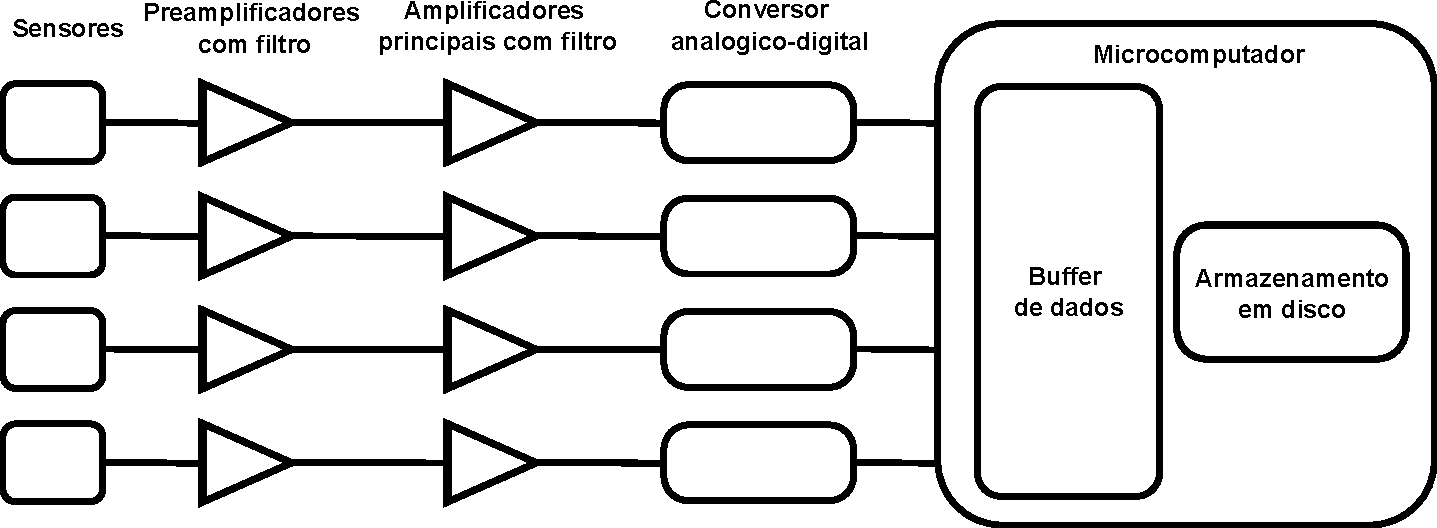
\includegraphics[width=.9\linewidth]{figs/Artigos/nde-ed-org/Figura1.pdf}
    \caption{Esquema funcional de um sistema de Emissão Acústica com sensores piezoelétricos, pré-amplificadores, filtros, amplificadores principais e sistema de aquisição digital. Adaptado de \citeonline{nde-ed-ae-equipment}.}
    \label{fig:nde-ed-org-Fig1}
\end{figure}

Inicialmente, os \textbf{sensores piezoelétricos} são fixados mecanicamente sobre a superfície do corpo de prova ou equipamento monitorado, utilizando acoplantes acústicos para otimizar a transmissão das ondas elásticas. Esses sensores são sensíveis a variações de pressão e deformações locais, produzindo um sinal elétrico \mbox{proporcional à amplitude da onda incidente}.

O sinal gerado pelo sensor é então encaminhado a um \textbf{pré-amplificador}, cuja função é elevar o nível de tensão do sinal original, geralmente na faixa de microvolts, para níveis adequados à posterior amplificação e filtragem. Em muitos sistemas, esse estágio inicial já incorpora filtros passa-faixa (tipicamente entre 100~kHz e 1~MHz), destinados a eliminar componentes de baixa frequência e ruídos ambientais, preservando apenas as frequências características dos eventos acústicos.

Em seguida, o sinal passa por um \textbf{amplificador principal}, também dotado de filtros ajustáveis, que permite o controle do ganho e a supressão de ruídos residuais. Essa dupla amplificação — pré e principal — é essencial para garantir uma relação sinal-ruído satisfatória, sobretudo em medições realizadas em ambientes industriais com \mbox{alta interferência eletromagnética.}

Após o condicionamento analógico, o sinal é direcionado a um \textbf{circuito de medição} que realiza a conversão analógico-digital, ADC, amostrando o sinal em altas taxas (geralmente entre 1~MHz e 40~MHz, dependendo da aplicação e do fenômeno estudado). Esses dados digitalizados são então armazenados temporariamente em um \textbf{\textit{buffer} de dados}, que atua como intermediário entre o \textit{front-end} analógico \mbox{e o sistema de processamento}.

O \textbf{microcomputador} ou unidade de controle central é responsável por gerenciar a aquisição e o armazenamento em disco, além de permitir o processamento dos sinais por meio de algoritmos dedicados à detecção de eventos, cálculo de parâmetros de emissão acústica (como amplitude, duração, energia e contagem de hits) e classificação de padrões. Em sistemas modernos, essa unidade também pode realizar a comunicação com interfaces externas, como APIs industriais, redes MODBUS ou sistemas supervisórios SCADA.

Por fim, o sistema é integrado a módulos de \textbf{visualização e controle}, permitindo que os resultados sejam exibidos em tempo real em um display ou monitor, e que o operador interaja por meio de um teclado ou interface gráfica. Essa visualização pode incluir formas de onda, histogramas de energia, espectros de frequência e alarmes automáticos quando limiares pré-definidos são excedidos.

Em conjunto, os elementos apresentados na Figura~\ref{fig:nde-ed-org-Fig1} compõem um sistema de aquisição e monitoramento de Emissão Acústica capaz de registrar, processar e analisar fenômenos transientes de alta frequência com elevada sensibilidade e precisão temporal. Esse tipo de arquitetura é amplamente empregado em pesquisas e aplicações industriais voltadas à detecção precoce de falhas estruturais, cavitação e fadiga de materiais, oferecendo uma alternativa não invasiva e altamente responsiva aos métodos tradicionais de inspeção.

Após a captação, o sinal adentra um circuito composto por \textbf{pré-amplificador}, \textbf{filtros} e \textbf{amplificador principal}, antes de ser \textbf{digitalizado} para análise computacional. Essa etapa é crucial porque eleva a relação sinal-ruído, atenua interferências eletromagnéticas e rejeita componentes espectrais alheios à banda de interesse; por essa razão, os pré-amplificadores costumam ser posicionados o mais próximo possível da fonte, reduzindo perdas por cabo e mitigando a suscetibilidade a ruídos acoplados.

A análise dos sinais de EA fornece dados cruciais por meio de parâmetros como \textbf{amplitude} (pico do sinal acima do nível de referência), \textbf{tempo de subida} (\textit{rise time}, usualmente do primeiro cruzamento de limiar ao pico), \textbf{duração} (intervalo durante o qual o sinal permanece acima do limiar), \textbf{contagens} (\textit{counts}, número de cruzamentos do limiar por um circuito comparador) e uma medida de \textbf{energia} associada ao evento. Na terminologia do \citeonline{nde-ed-ae-equipment}, essa energia é frequentemente chamada de \textbf{MARSE} (\textit{measured area under the rectified signal envelope}) e corresponde, de forma simplificada, à \textit{área sob o invólucro retificado} do sinal durante a janela do evento; detalhes são esquematizados na Figura~\ref{fig:nde-ed-org-Fig2}. Tais parâmetros não apenas permitem identificar e caracterizar “\textit{hits}” de emissão, mas também se prestam à separação entre ocorrências significativas e ruído de fundo, funcionando como indicadores robustos dos mecanismos físicos subjacentes ao dano.

\begin{figure}[H]
    \centering
    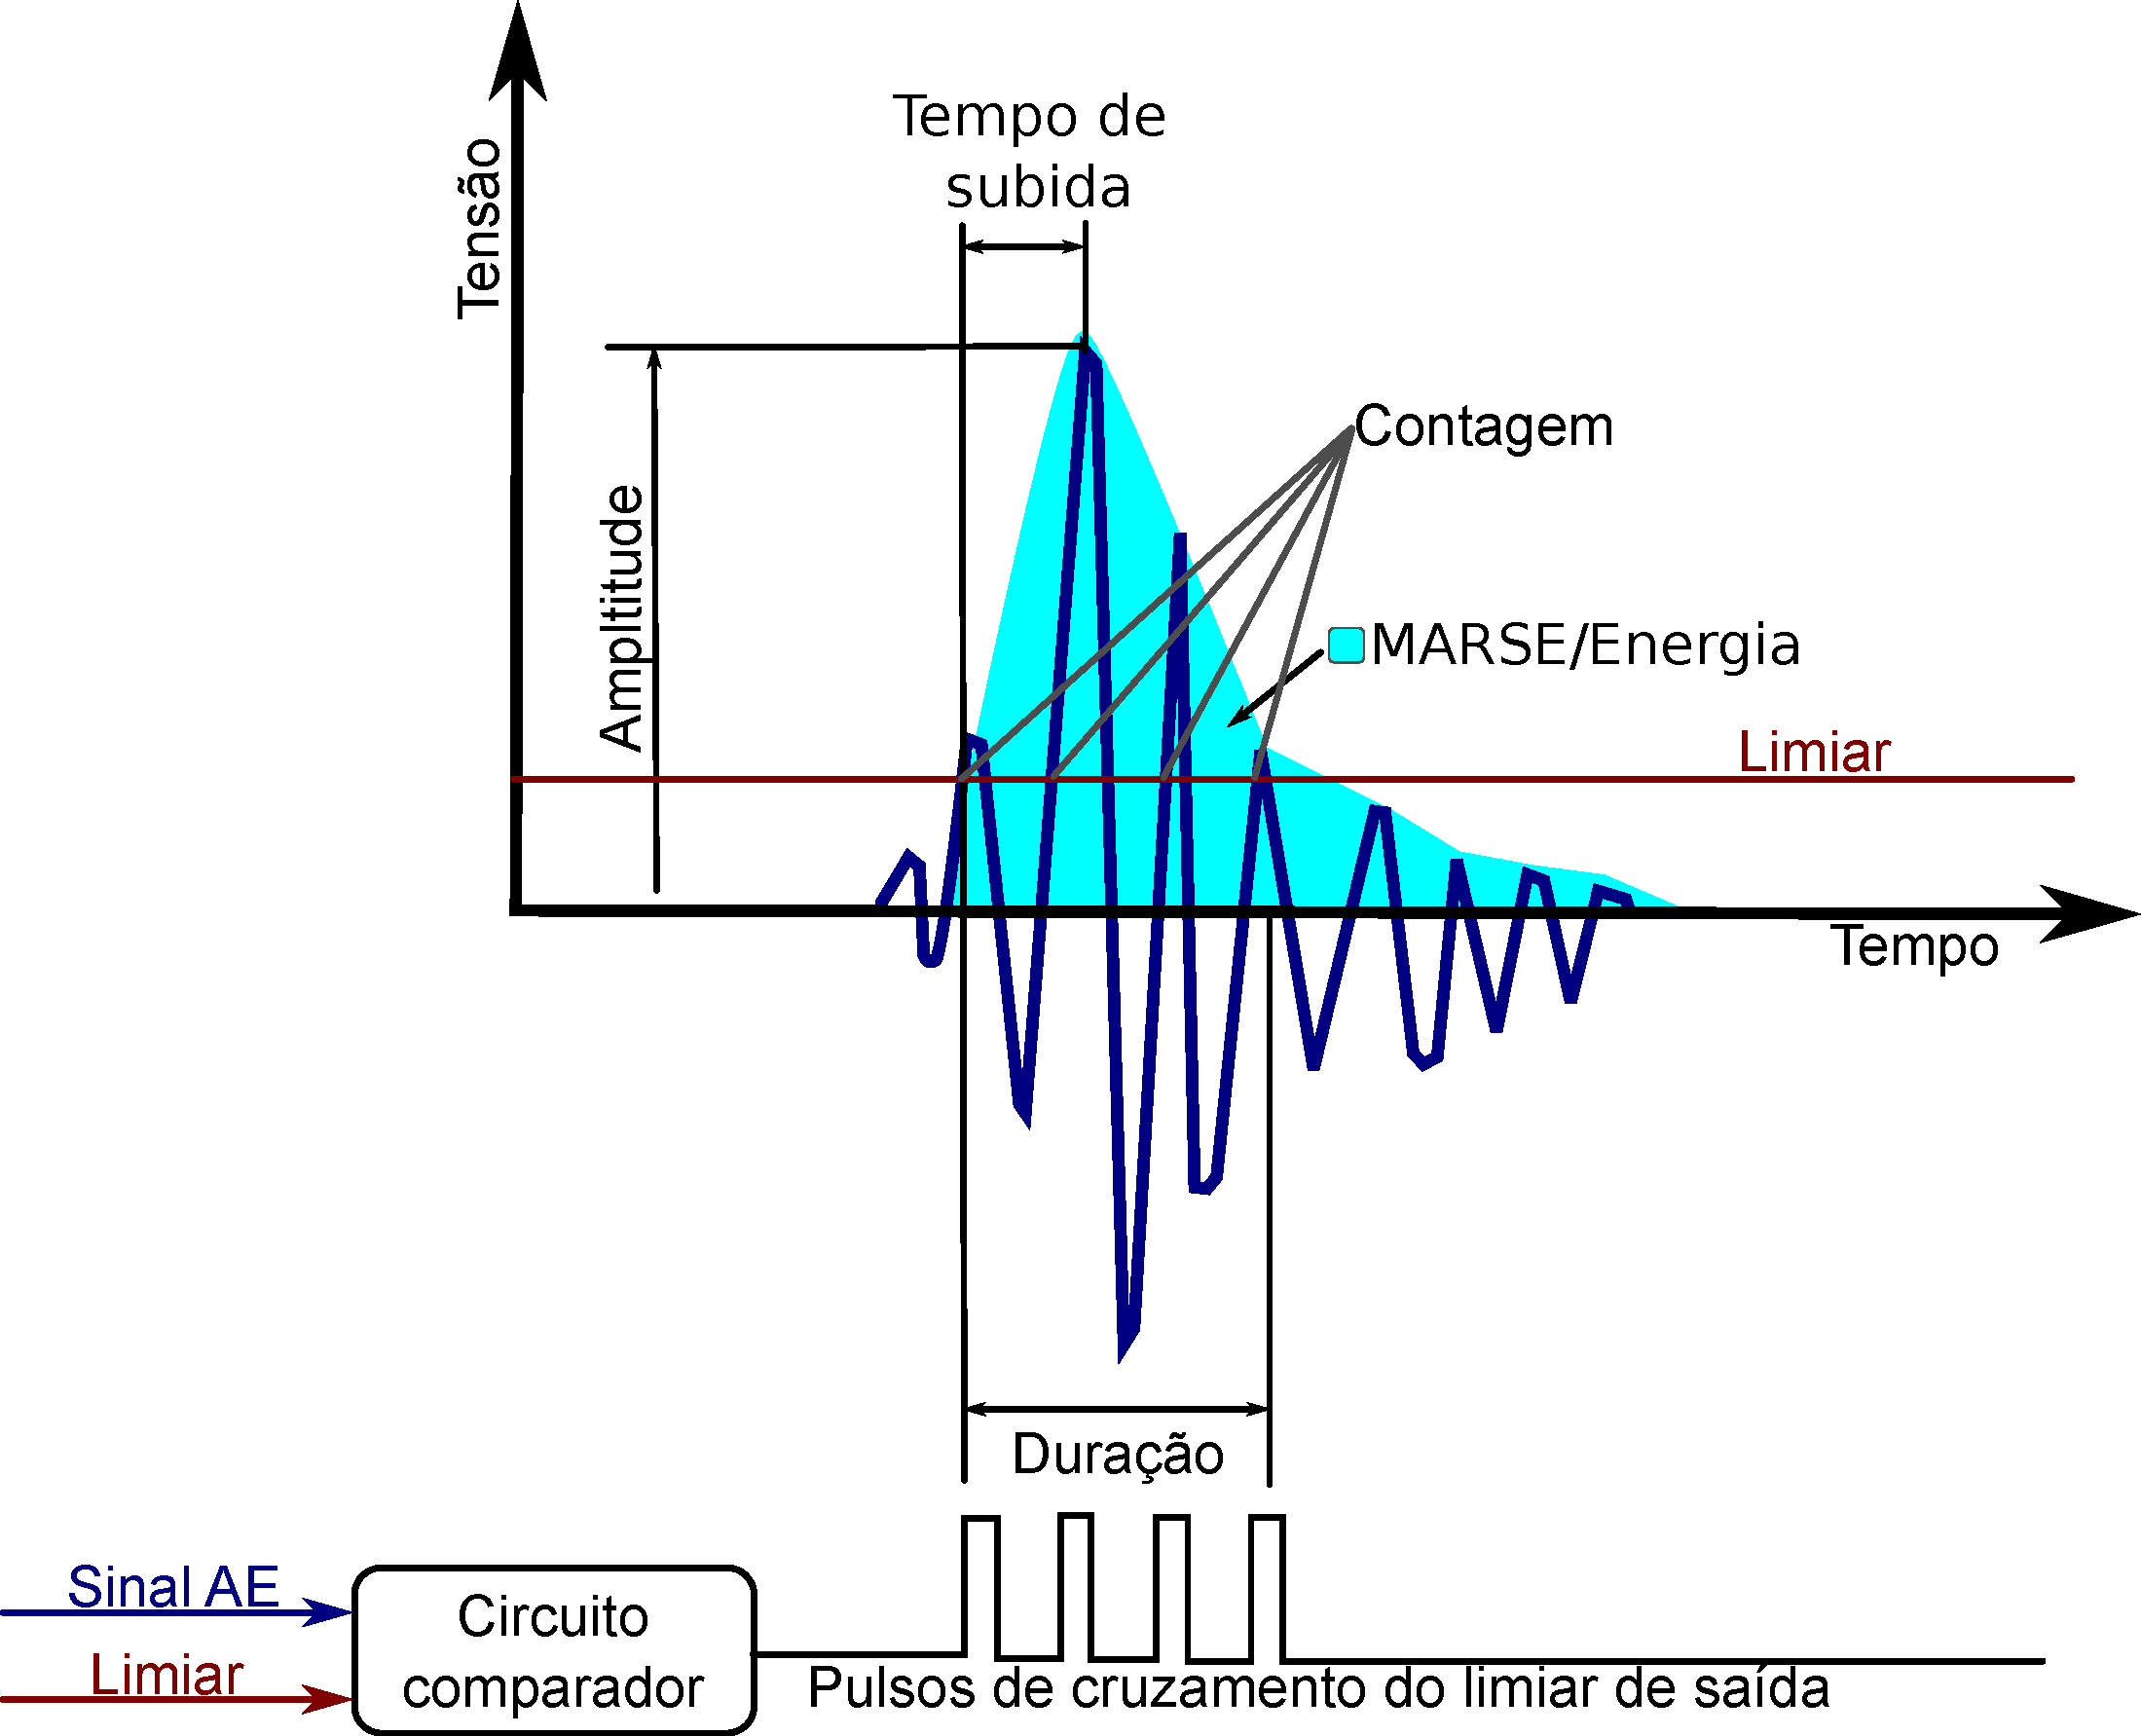
\includegraphics[width=.7\linewidth]{figs/Artigos/nde-ed-org/Figura2.pdf}
    \caption{Parâmetros clássicos extraídos de um “hit” de EA: amplitude, tempo de subida (\textit{rise time}), duração, contagens de limiar (\textit{counts}) e medida de energia (MARSE). O circuito comparador gera pulsos a cada cruzamento do limiar, contabilizados pelo sistema (adaptado de \citeonline{nde-ed-ae-equipment}).}
    \label{fig:nde-ed-org-Fig2}
\end{figure}

Do ponto de vista operacional, o \textbf{limiar} (\textit{threshold}) é definido sobre o nível de ruído para que a detecção seja seletiva. Um \textbf{hit} inicia no primeiro cruzamento desse limiar e se encerra quando o sinal permanece abaixo dele por um tempo de \textit{hit lockout} pré-definido. A partir daí, decompõem-se as grandezas:
\begin{itemize}
    \item \textbf{Amplitude} ($A_\text{pico}$): valor máximo do sinal acima do nível de referência dentro do hit.
    \item \textbf{Tempo de subida} ($t_\text{rise}$): intervalo do primeiro cruzamento de limiar até $A_\text{pico}$; é sensível à cinemática da fonte e à resposta do caminho de propagação.
    \item \textbf{Duração} ($t_\text{dur}$): tempo entre o primeiro e o último cruzamento do limiar; aumenta na presença de reverberações e múltiplas reflexões.
    \item \textbf{Contagens} (\textit{counts}): número de pulsos gerados pelo comparador a cada cruzamento de limiar; correlaciona-se com o conteúdo de alta frequência e a “granulosidade” do evento.
    \item \textbf{Energia (MARSE)}: área sob o invólucro retificado do sinal dentro da janela do hit.Matematicamente, a forma \textit{MARSE} pode ser escrita, em uma discretização simples,~como apresentada em \ref{eq:marse}. 
    
    \begin{equation}
    	\label{eq:marse}
    	\text{MARSE} \;\approx\; \sum_{n=n_0}^{n_1} \big|\,x[n]\,\big| \;\Delta t
    	\quad\text{ou}\quad
    	\text{MARSE} \;\approx\; \sum_{n=n_0}^{n_1} e[n] \;\Delta t,
    \end{equation}
    %$$
    %\text{MARSE} \;\approx\; \sum_{n=n_0}^{n_1} \big|\,x[n]\,\big| \;\Delta t
    %\quad\text{ou}\quad
    %\text{MARSE} \;\approx\; \sum_{n=n_0}^{n_1} e[n] \;\Delta t,
    %$$
    
    em que $x[n]$ é o sinal de EA amostrado e $e[n]$ denota o invólucro (por exemplo, obtido por retificação + filtragem passa-baixas, ou por transformada de Hilbert). Essa métrica captura \textit{quanta de atividade} ao longo do hit, sendo bastante utilizada por fornecedores de instrumentação de EA e por materiais de referência \mbox{educacionais como o \citeonline{nde-ed-ae-equipment}.}
\end{itemize}

\noindent\textbf{{Observação sobre nomenclatura de energia.}}

É importante salientar que \textbf{não há consenso terminológico} na literatura quanto à ``energia'' do evento de EA. Enquanto o \citeonline{nde-ed-ae-equipment} emprega \textit{MARSE} (área do invólucro retificado), revisões de estado da arte, como \citeonline{liu2023review}, frequentemente utilizam \textbf{energia baseada em potência instantânea}, aproximada pela soma dos quadrados da amplitude (proporcional a energia acústica sob hipóteses de linearidade do caminho e calibração adequada, \mbox{como apresentada em \ref{eq:energia}:}

\begin{equation}
	\label{eq:energia}
	E_\text{sq} \;\propto\; \sum_{n=n_0}^{n_1} x^2[n] \;\Delta t.
\end{equation}

Em aplicações comparativas,por exemplo, na distinção entre cavitação incipiente e regimes estabelecidos,essa diferença \textit{conceitual} pode impactar limiares de decisão, escalas de normalização e correlações com grandezas físicas. Por isso, ao longo desta dissertação, quando nos referirmos a \textbf{MARSE}, estaremos explicitamente adotando a \textit{área do invólucro retificado}; quando nos referirmos à \textbf{energia quadrática} (ou simplesmente “energia” na acepção de \citeonline{liu2023review}), estaremos empregando a soma dos quadrados da amplitude. Sempre que pertinente, serão fornecidas ambas as métricas, devidamente normalizadas, de modo a preservar a comparabilidade com diferentes fontes bibliográficas e práticas~de~instrumentação.


O diferencial da técnica reside em seu caráter passivo — ela ``ouve'' a emissão real do material sob carga, ao invés de estimular o componente, como ocorre em métodos como ultrassom ou radiografia. Isso permite monitoramento contínuo e não intrusivo em condições operacionais reais, captando apenas fontes ativas de dano e cobrindo grandes volumes estruturais com um número reduzido de sensores.

Além disso, sistemas de EA podem operar com localização acústica da fonte emissora, utilizando redes de sensores e analisando as diferenças de tempo de chegada do sinal (métodos linear, planar ou volumétrico), o que permite determinar a posição exata de emissão dentro da estrutura.

Esses parâmetros, além de fornecerem informações físicas sobre a natureza do evento, constituem também a base para a extração de \textit{features} no contexto de aprendizado de máquina. Em abordagens modernas de análise de sinais de Emissão Acústica, como a proposta neste trabalho, o conjunto de atributos derivados desses parâmetros — tanto no domínio do tempo quanto no domínio da frequência — é utilizado para representar cada evento (\textit{hit}) de forma compacta e informativa, facilitando sua posterior~classificação~por~redes neurais.

No domínio do tempo, são extraídos descritores diretos, como amplitude, duração, tempo de subida, energia (MARSE ou energia quadrática), número de contagens e razão entre parâmetros (por exemplo, a razão entre energia e duração, indicativa da intensidade relativa do evento). Já no domínio da frequência, técnicas de análise espectral, como a Transformada Rápida de Fourier (FFT) ou a Transformada de Short-Time Fourier (STFT), permitem a identificação de componentes dominantes e a distinção entre regimes acústicos característicos — como cavitação incipiente, cavitação plena e ruído mecânico.

Durante o pré-processamento, esses parâmetros são normalizados com base em janelas móveis e limiares de ruído, garantindo que variações instrumentais ou ambientais não influenciem indevidamente o processo de aprendizagem. As janelas de tempo são segmentadas e rotuladas conforme as classes de operação (\textit{normal}, \textit{cavitação} ou \textit{falha estrutural}), e o conjunto de sinais normalizados é então utilizado como \mbox{entrada para o treinamento da CNN-1D.}

Nesse contexto, a rede convolucional atua como uma extensão automática do processo de extração de \textit{features}, aprendendo representações hierárquicas diretamente das formas de onda ou dos espectrogramas derivados. Essa combinação entre parâmetros clássicos da Emissão Acústica e aprendizado profundo forma uma abordagem híbrida que alia a interpretabilidade dos métodos tradicionais à robustez e adaptabilidade dos modelos modernos de Inteligência Artificial, conforme ilustrado no fluxograma geral dos objetivos~da pesquisa (Figura~\ref{fig:fluxograma_geral}).

Ademais, a onda primitiva originada em um evento de EA é tipicamente de curta duração (microssegundos) e pode apresentar forte direcionalidade e variabilidade na amplitude, dependendo da natureza física da falha, como deformação cristalina ou fraturas progressivas. Sua propagação é influenciada por fatores como atenuações geométricas, estruturais e pela dispersão devido à microestrutura do material, \mbox{como os contornos de grão e inclusões.}

É importante ressaltar que nem toda emissão EA indica falha estrutural: fenômenos como fricção mecânica, vazamentos e pulsos por cavitação ou descargas parciais podem produzir sinais semelhantes aos genuínos, classificados como pseudo-fontes. A aplicação de filtros avançados, avaliação espectral e critérios baseados em tempo de chegada são estratégias fundamentais para distinguir esses eventos e minimizar falsos positivos.

Em síntese, a técnica de Emissão Acústica apresenta-se como uma abordagem promissora para o monitoramento em tempo real e a detecção precoce de falhas estruturais, devido à sua alta sensibilidade e natureza não intrusiva. A compreensão de seus princípios físicos e dos parâmetros característicos extraídos dos sinais é essencial para a correta interpretação dos fenômenos observados, como trincas, desgaste superficial e cavitação em bombas centrífugas. A seguir, são discutidos estudos representativos que exploram a aplicação da Emissão Acústica em sistemas hidráulicos e turbomáquinas, evidenciando as metodologias empregadas, os resultados obtidos e as limitações que \mbox{motivam o presente~trabalho.}

\subsection{Revisão de Pesquisas sobre Emissão Acústica}

Segundo \citeonline{liu2023review}, a cavitação em bombas é um fenômeno multifásico inevitável que provoca a formação e colapso de bolhas quando a pressão local do escoamento cai abaixo da pressão de vapor do líquido. Esse processo resulta em perda de desempenho hidráulico, erosão de componentes, vibração excessiva e ruído característico, podendo até gerar falhas estruturais. A detecção precoce, portanto, tem grande relevância tanto para a segurança operacional quanto para a redução de custos de manutenção.

Os autores revisam diferentes metodologias de detecção baseadas em sinais, como vibração, emissão acústica, ruído hidrodinâmico e pulsação de pressão. Conforme ilustrado no fluxograma da Figura~\ref{fig:LiuFig1}, tais métodos seguem um fluxo comum: aquisição de sinais em pontos estratégicos da bomba, processamento nos domínios do tempo, frequência ou tempo–frequência, extração de parâmetros característicos e, por fim, identificação do estado de cavitação com auxílio de algoritmos de inteligência artificial. A Figura~\ref{fig:LiuFig2} resume essas metodologias de pesquisa.

\begin{figure}[H]
    \centering
    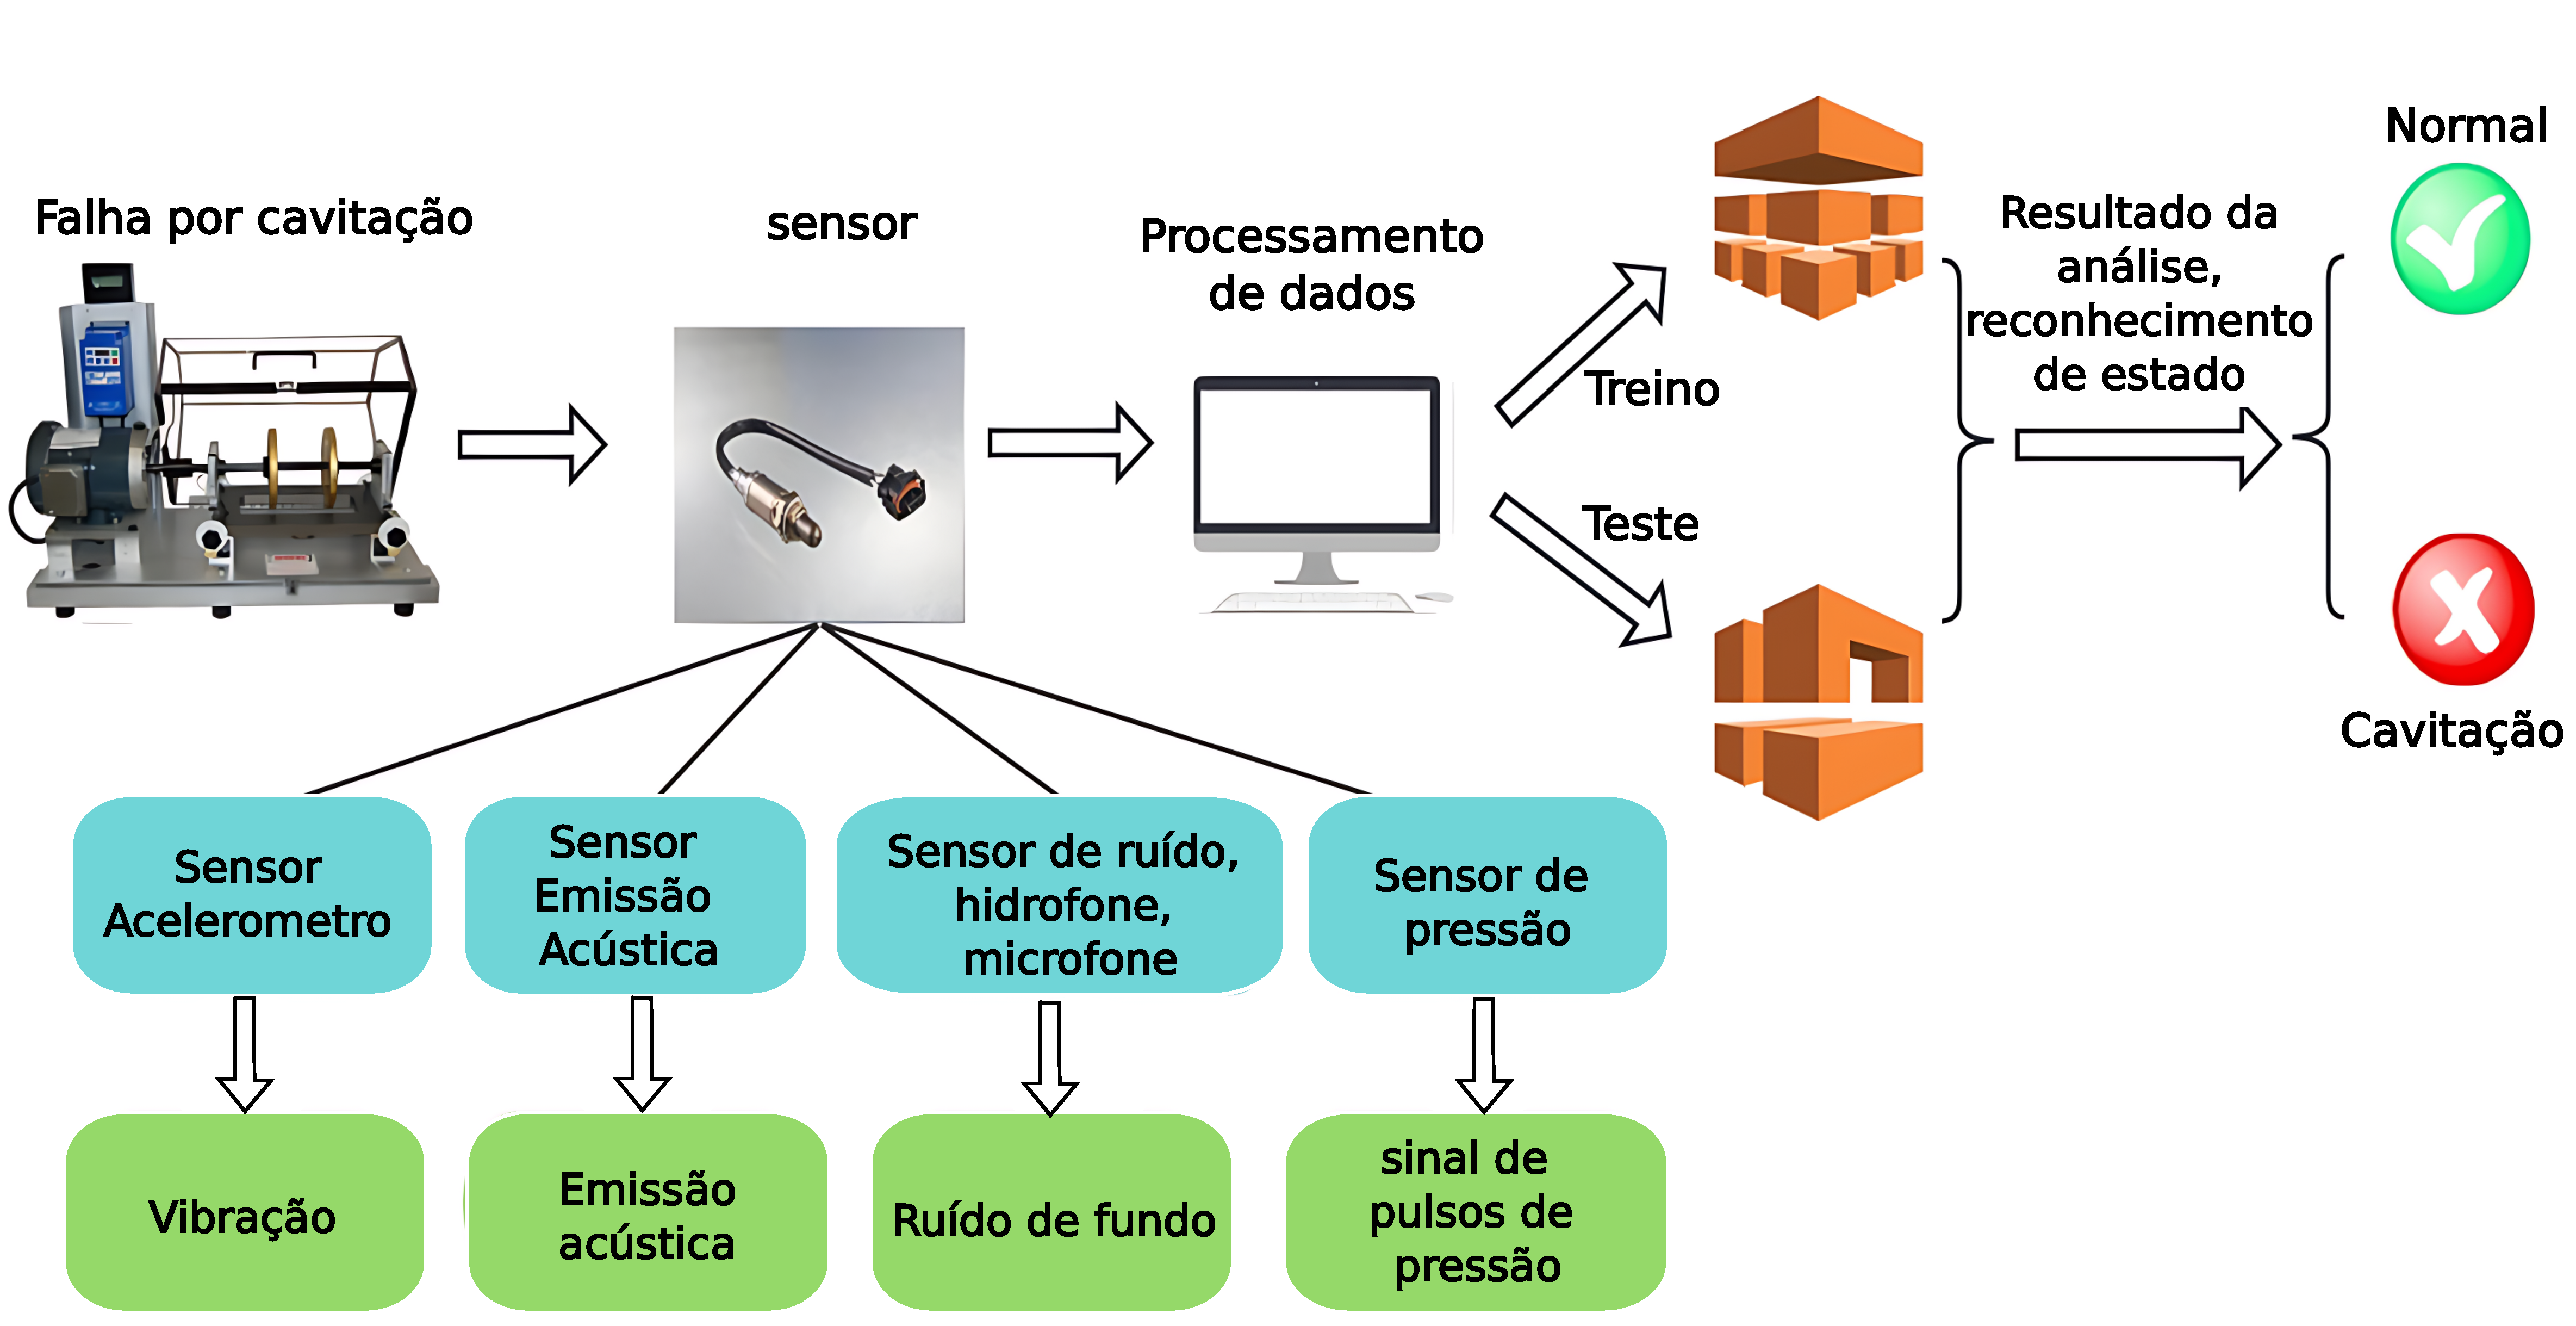
\includegraphics[width=1\linewidth]{figs/Artigos/Liu/Figura1.pdf}
    \caption{Fluxograma básico de detecção de cavitação com base em diferentes sinais. Adaptado de \citeonline{liu2023review}.}
    \label{fig:LiuFig1}
\end{figure}

O diagrama da Figura~\ref{fig:LiuFig1} organiza a detecção por \textbf{famílias de sinais} e explicita a relação entre a física da cavitação e o canal sensorial:
\begin{itemize}
    \item \textbf{Sinal de vibração (acelerômetros):} sensível à excitação mecânica do conjunto rotor–estator; captura impactos e modulações de banda larga provocadas pelo colapso de bolhas e por fenômenos associados, entre outros efeitos (desbalanceamento secundário, instabilidades hidráulicas).
    
    \item \textbf{Sinal de emissão acústica (sensores piezoelétricos):} focaliza faixas de alta frequência (tipicamente centenas de kHz), nas quais eventos transientes de cavitação apresentam razão sinal–ruído elevada; adequado à detecção incipiente.
    \item \textbf{Sinal de ruído (microfones/hidrofones):} capta componentes aéreas ou no fluido; informativo para estágios mais intensos de cavitação e para varreduras rápidas, embora mais suscetível a interferências ambientais.
    \item \textbf{Pulsação de pressão (transdutores de pressão):} evidencia flutuações periódicas/quasi-periódicas do campo de pressão; útil para mapear regimes e instabilidades do escoamento.
\end{itemize}
A linha intermediária do diagrama explicita que \textbf{cada sensor observa um aspecto da cavitação}: os sinais carregam assinaturas distintas (impactos, bandas espectrais, intermitência, modulações). A partir daí, o fluxo converge para \textbf{processamento de sinais} (métricas no tempo: RMS, pico, curtose, crest factor; no espectro: centroides, bandas energéticas; no tempo–frequência: STFT, wavelets), seguido de \textbf{extração de atributos} e \textbf{reconhecimento de estado} por algoritmos de IA (por exemplo, \textit{SVM}, \textit{Random Forest}, \textit{k-NN}, e redes profundas como CNN-1D/2D ou \textit{LSTM}). Em síntese, a figura mostra que, embora os canais sensoriais sejam diversos, o \textit{pipeline lógico} é comum e modular.

\begin{figure}[H]
    \centering
    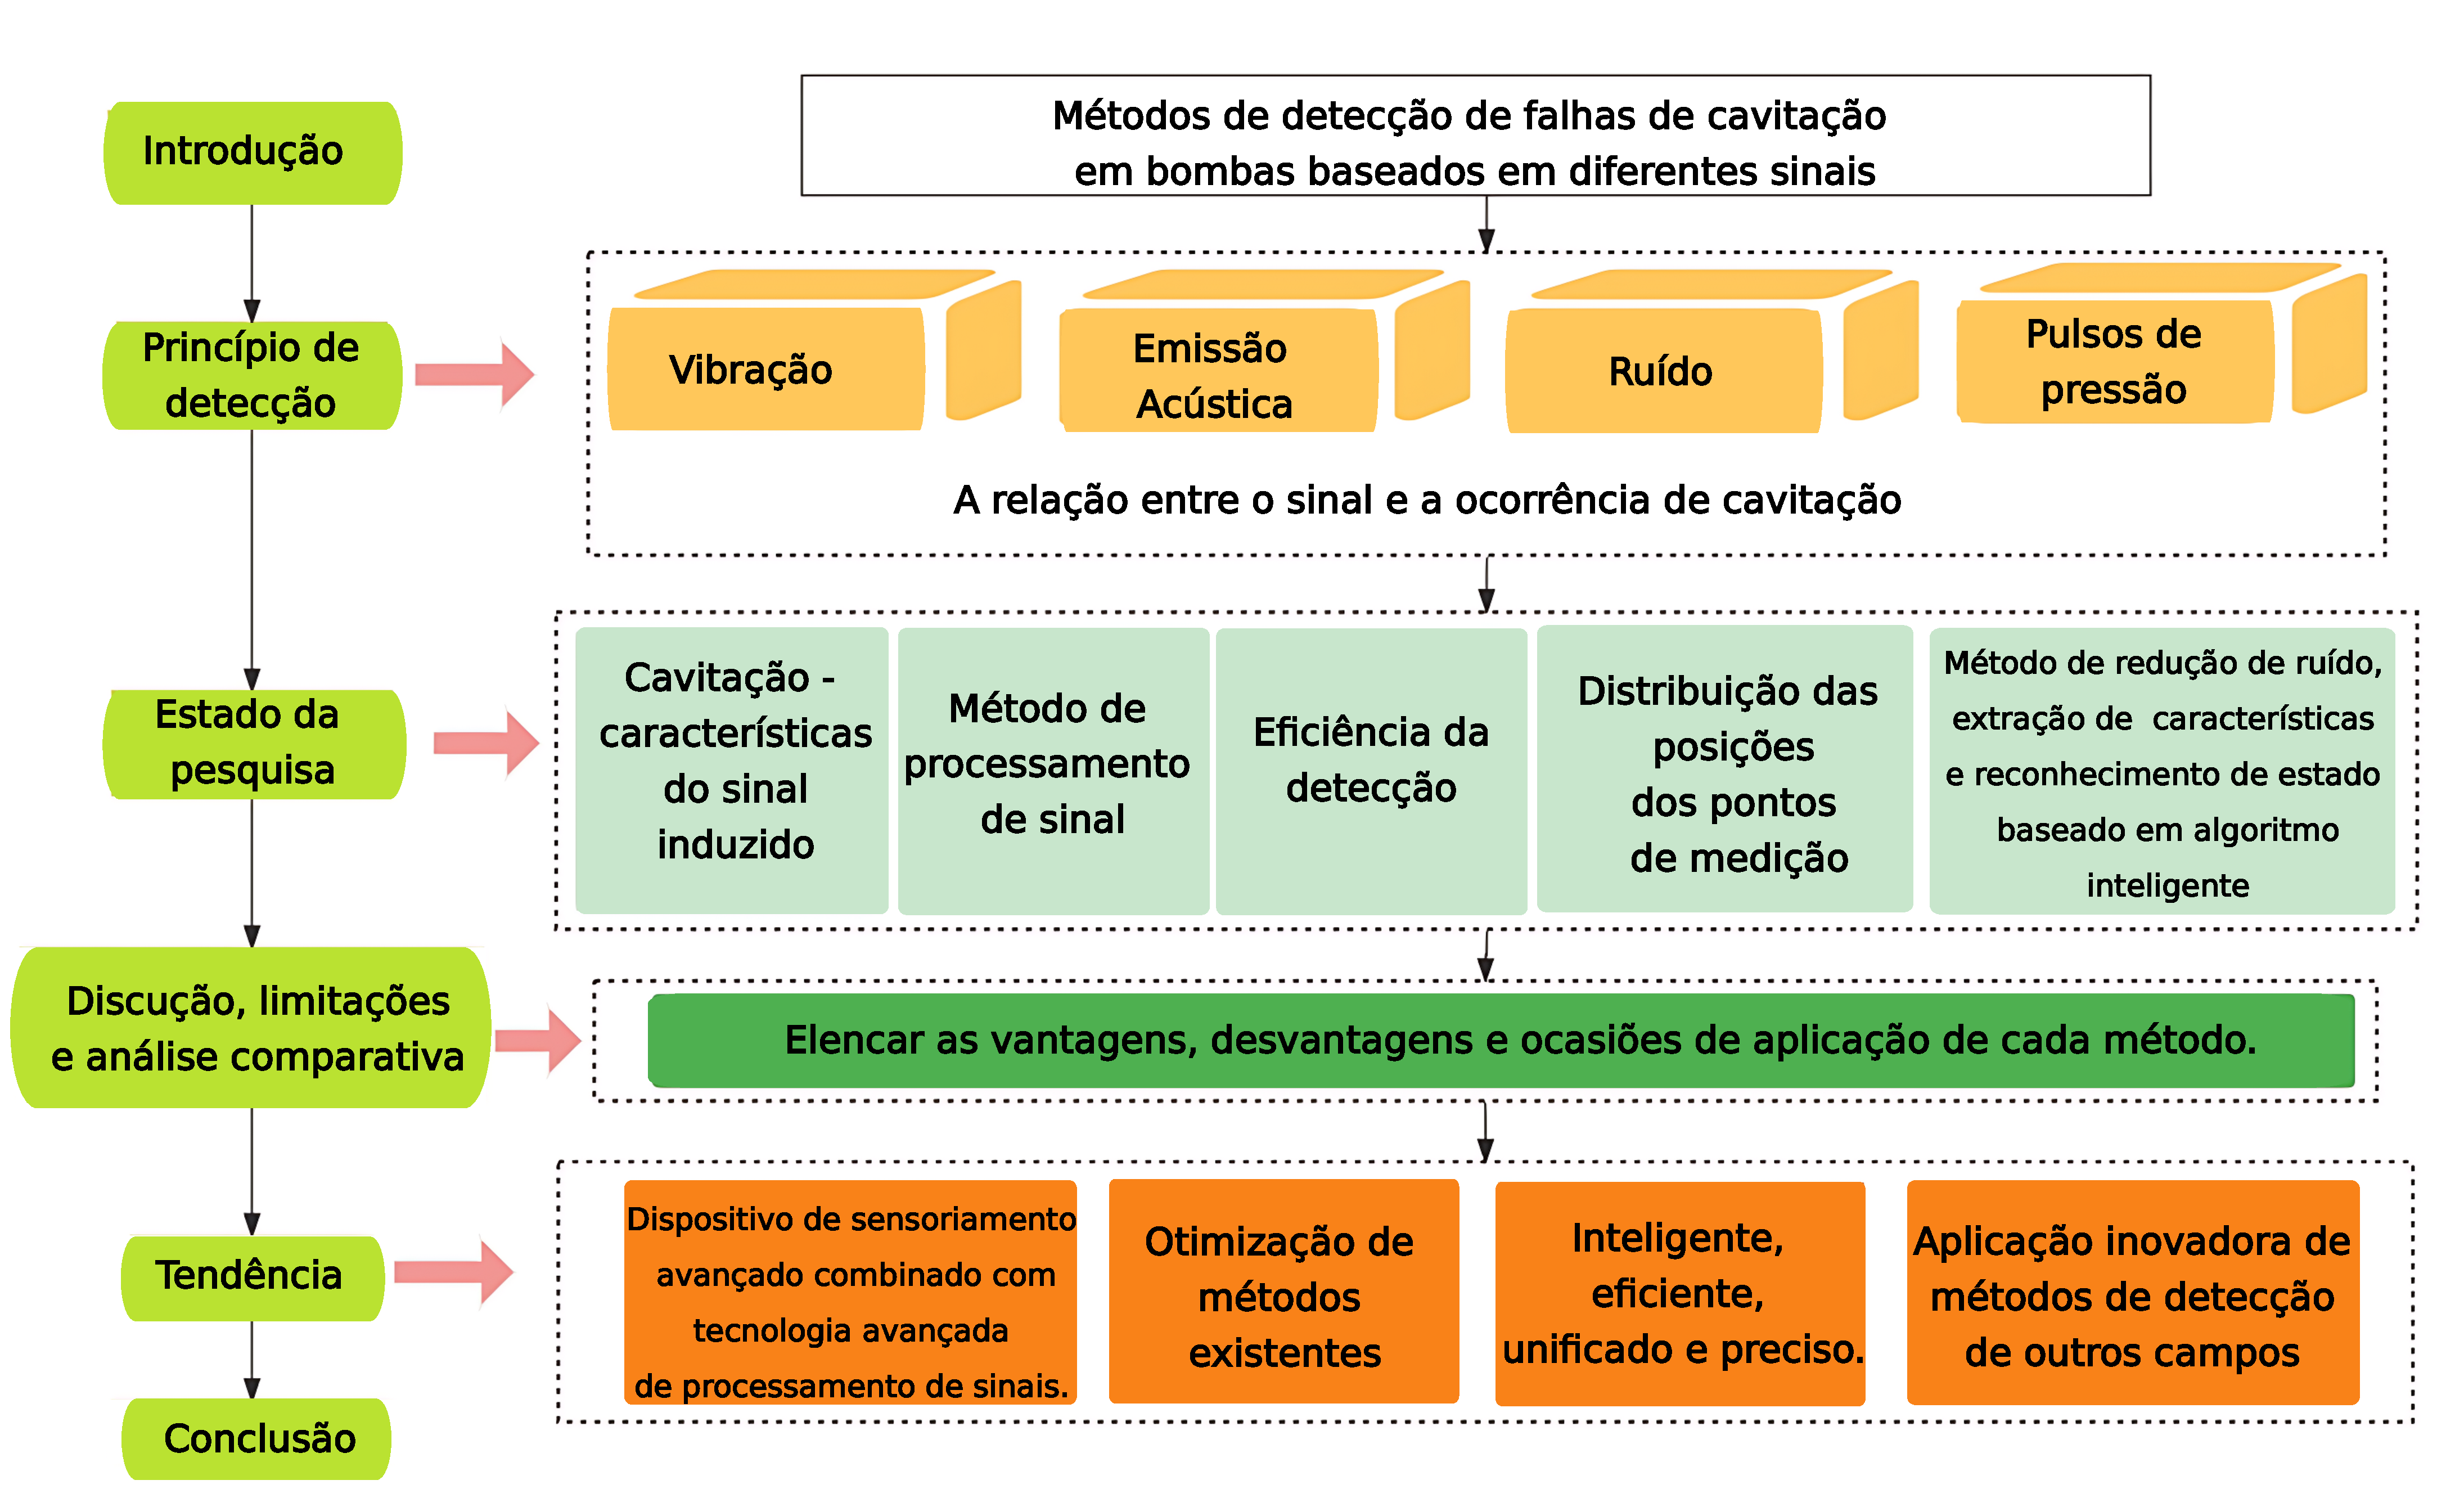
\includegraphics[width=1\linewidth]{figs/Artigos/Liu/Figura2.pdf}
    \caption{Diagrama principal do conteúdo da pesquisa do artigo. Adaptado de \citeonline{liu2023review}. }
    \label{fig:LiuFig2}
\end{figure}

Com o objetivo de mapear os desafios do monitoramento de condição, o esquema ilustrado na Figura~\ref{fig:LiuFig2} sintetiza o \textbf{ciclo de pesquisa} em cinco camadas essenciais. Tal segmentação abrange desde a caracterização do problema de desempenho e integridade em bombas até a implementação de soluções inteligentes unificadas, compreendendo os seguintes tópicos:

\linespread{1.27}\selectfont
\begin{enumerate}
    \item \textbf{Introdução:} contextualiza a cavitação como problema de desempenho e integridade; define objetivos (detecção incipiente, redução de custos, aumento de confiabilidade).
    \item \textbf{Princípio de detecção:} relaciona a \textit{origem física} da cavitação com o \textit{que cada sensor enxerga}. Por exemplo, o colapso de bolhas gera altas frequências (AE), enquanto flutuações de pressão se refletem mais nos transdutores de pressão e na vibração de baixa/média frequência.
    \item \textbf{Estado da pesquisa:} quatro eixos críticos:
    \begin{enumerate}[label=\alph*)]
        \item \textit{Características induzidas pela cavitação:} intermitência, assimetria estatística, picos espectrais e alargamento de banda; mudanças em curtose, entropias e taxas de cruzamento por limiar.
        \item \textit{Métodos de processamento de sinais:} do básico (filtros, estatísticas de ordem superior) ao avançado (STFT, CWT, espectrogramas, \textit{scalograms}, cepstra).
        \item \textit{Eficiência de detecção:} métricas (acurácia, sensibilidade, especificidade, AUC, F1), além de latência e robustez a ruído; aqui entram comparações sistemáticas entre algoritmos e sensores.
        \item \textit{Posicionamento de pontos de medição:} trade-offs entre proximidade do fenômeno, acessibilidade, segurança, custo e suscetibilidade a ruído estrutural/ambiental.
    \end{enumerate}
    \item \textbf{Discussão, limitações e comparação:} consolida \textit{vantagens e desvantagens} de cada canal/sensor: AE destaca-se na detecção incipiente e em altas frequências, vibração é amplamente disponível e barata, pressão é direta para regimes hidráulicos, ruído é fácil de instrumentar porém sensível a ambiente. Também discute limitações (calibração, variabilidade do escoamento, repetibilidade, datasets pequenos).
    \item \textbf{Tendências:} quatro direções estratégicas:
    \begin{enumerate}[label=\alph*)]
        \item \textit{Sensoriamento avançado + processamento avançado:} sensores banda-larga, arrays, sincronização multicanal; pipelines tempo–frequência e fusão multimodal.
        \item \textit{Otimização de métodos existentes:} melhor seleção de \textit{features}, redução de dimensionalidade, aprendizado semi-supervisionado e \textit{few-shot}.
        \item \textit{Sistemas inteligentes, unificados e acurados:} do laboratório ao campo, com atenção à \textbf{latência}, \textbf{robustez a ruído} e \textbf{generalização} entre bombas/condições.
        \item \textit{Transferência de métodos de outras áreas:} técnicas maduras de diagnóstico de máquinas, sonar/ultrassom e visão computacional (ex., CNNs 1D/2D, transformers específicos para séries temporais).
    \end{enumerate}
\end{enumerate}


Em síntese, as Figuras \ref{fig:LiuFig1} e \ref{fig:LiuFig2} evidenciam que a detecção de cavitação tem evoluído de abordagens puramente empíricas para arquiteturas \textbf{modulares e orientadas a dados}, nas quais a escolha do sensor, a estratégia de processamento e o modelo de classificação integram-se em um \textit{pipeline} unificado e flexível. Essa estrutura permite adaptar metodologias de diagnóstico a distintos contextos industriais, conciliando precisão, \mbox{tempo de resposta e viabilidade de implementação.}

Sob essa perspectiva, os estudos analisados reforçam a motivação central desta pesquisa: investigar a cadeia de processamento que envolve o \textbf{pré-processamento}, a \textbf{extração e representação de atributos} e a \textbf{classificação por meio de uma CNN-1D}, com o objetivo de alcançar uma detecção de cavitação rápida, robusta e energeticamente eficiente. Ao mesmo tempo, mantém-se a perspectiva de integração futura dessas técnicas em \textit{hardware} reconfigurável, consolidando um caminho viável para soluções embarcadas de monitoramento inteligente.


Entre os diversos métodos analisados por \citeonline{liu2023review}, o monitoramento por vibração se destaca como o mais consolidado e amplamente aplicado em sistemas hidráulicos industriais. Alterações expressivas na resposta espectral, especialmente o surgimento de picos em faixas de 2 kHz a 8 kHz, constituem indicadores diretos da presença de cavitação — fenômeno ilustrado nas Figuras \ref{fig:LiuFig4A} e \ref{fig:LiuFig4B}. A primeira demonstra a diferença temporal entre regimes de operação com e sem cavitação, evidenciando o aumento abrupto da amplitude e da irregularidade do sinal. Já a segunda mostra, no domínio da frequência, o deslocamento da energia espectral e a intensificação de componentes harmônicas conforme a rotação da bomba aumenta, comportamento que reflete a instabilidade hidrodinâmica \mbox{provocada pelo colapso das bolhas.}

Apesar de sua maturidade tecnológica, o método de vibração apresenta sensibilidade limitada à cavitação incipiente, uma vez que os sinais gerados nos estágios iniciais do fenômeno são de baixa amplitude e facilmente mascarados por ruídos mecânicos ou estruturais. Nesse contexto, a técnica de \textbf{Emissão Acústica, EA} desponta como alternativa mais sensível e informativa. Essa abordagem capta as ondas elásticas transitórias geradas por microjatos e choques associados ao colapso de cavidades, abrangendo uma faixa espectral que se estende de aproximadamente 1 kHz a 1 MHz.

Os parâmetros derivados do sinal, como \textbf{amplitude}, \textbf{duração}, \textbf{energia} e \textbf{contagens acima do limiar} (ou “counts”), mostrados na Figura \ref{fig:LiuFig6}, constituem indicadores diretos da intensidade e da frequência de ocorrência dos eventos acústicos. Esses parâmetros — amplamente empregados em sistemas de monitoramento baseados em hits — permitem não apenas detectar a cavitação incipiente, mas também avaliar a severidade do processo de erosão associada. No entanto, sua adoção em ambientes industriais ainda é desafiada por fatores como o custo dos sensores piezoelétricos de alta sensibilidade, a necessidade de acoplamento preciso e a suscetibilidade à interferência estrutural.

Assim, enquanto os sensores de vibração oferecem uma visão global e robusta do comportamento dinâmico do conjunto rotativo, a emissão acústica fornece uma janela privilegiada para o diagnóstico precoce, sendo particularmente promissora para integração futura com plataformas embarcadas de detecção inteligente — foco desta pesquisa.
\linespread{1.25}\selectfont

\begin{figure}[H]
    \centering
    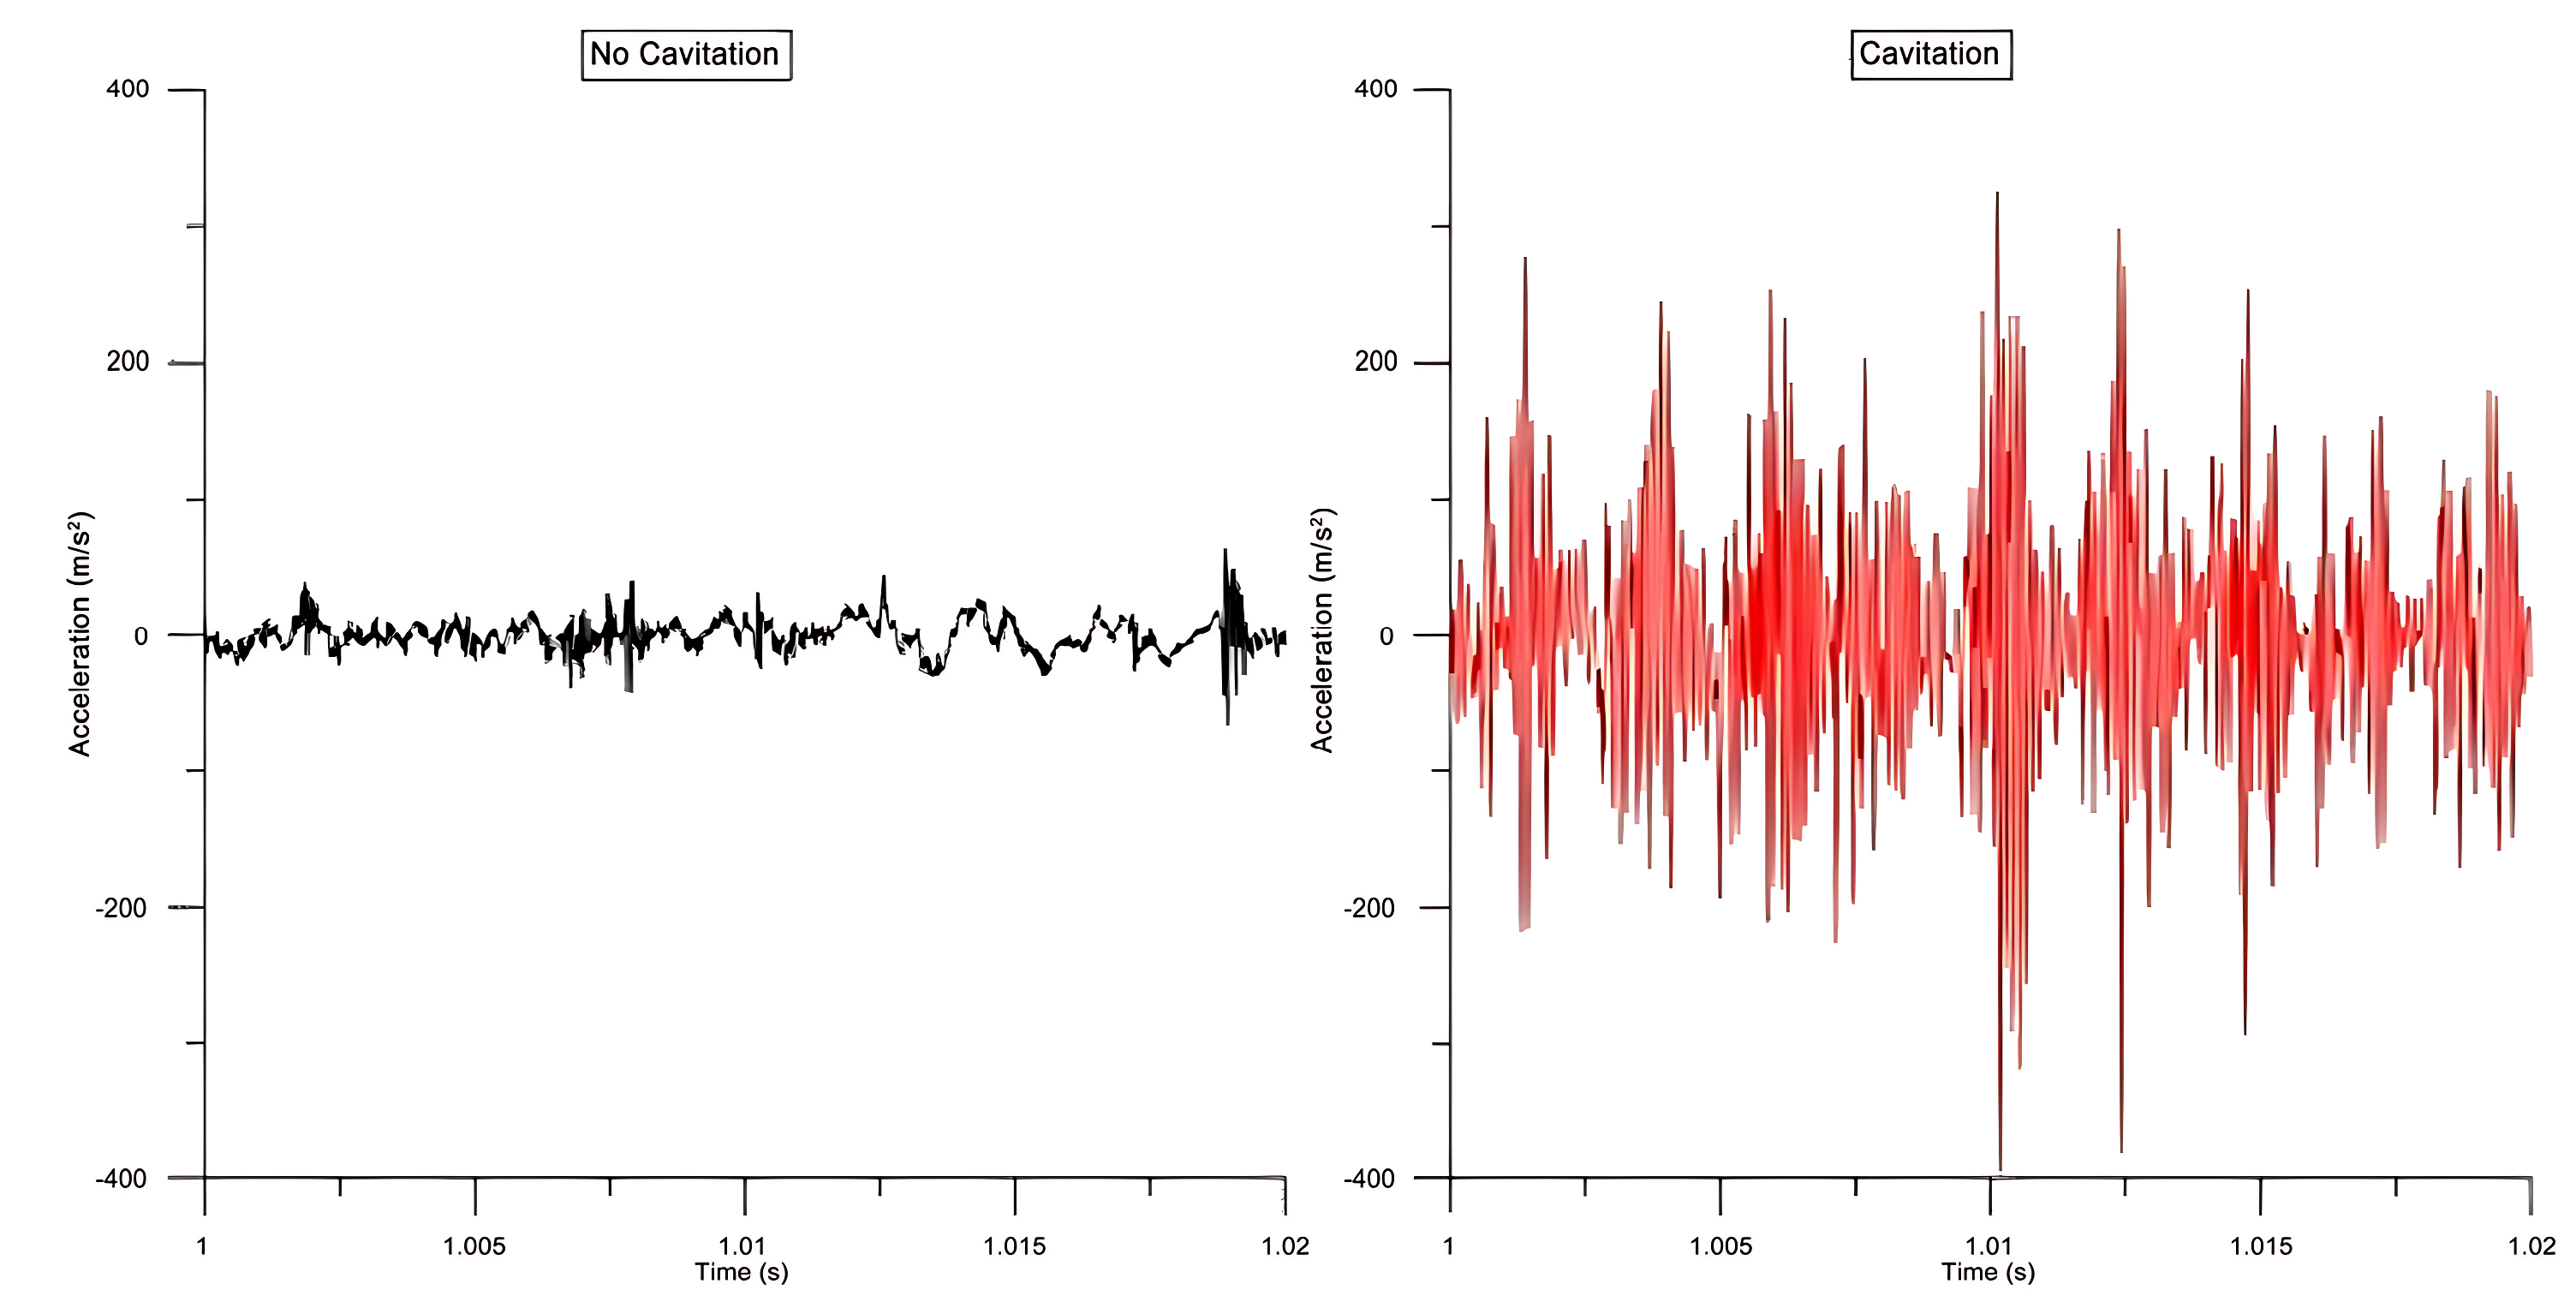
\includegraphics[width=0.95\linewidth]{figs//Artigos//Liu/Figura4A_Upscaler_2K.png}
    \caption{Sinais de aceleração no domínio do tempo em estados de cavitação e não cavitação. Fonte: \citeonline{liu2023review}}
    \label{fig:LiuFig4A}
\end{figure}

A Figura \ref{fig:LiuFig4A} apresenta os sinais de aceleração medidos em uma bomba centrífuga em duas condições distintas: à esquerda, operação normal (sem cavitação), e à direita, sob cavitação. Observa-se que o regime sem cavitação exibe um sinal estável, de baixa amplitude e com pequenas variações associadas ao ruído de fundo e às vibrações naturais da máquina. Em contrapartida, o regime cavitante demonstra um aumento expressivo na amplitude e na irregularidade temporal do sinal, reflexo direto do colapso das bolhas de vapor dentro do fluido. Esse comportamento errático é característico da cavitação e se intensifica com o aumento da velocidade de rotação e da severidade do fenômeno.

\begin{figure}[H]
    \centering
    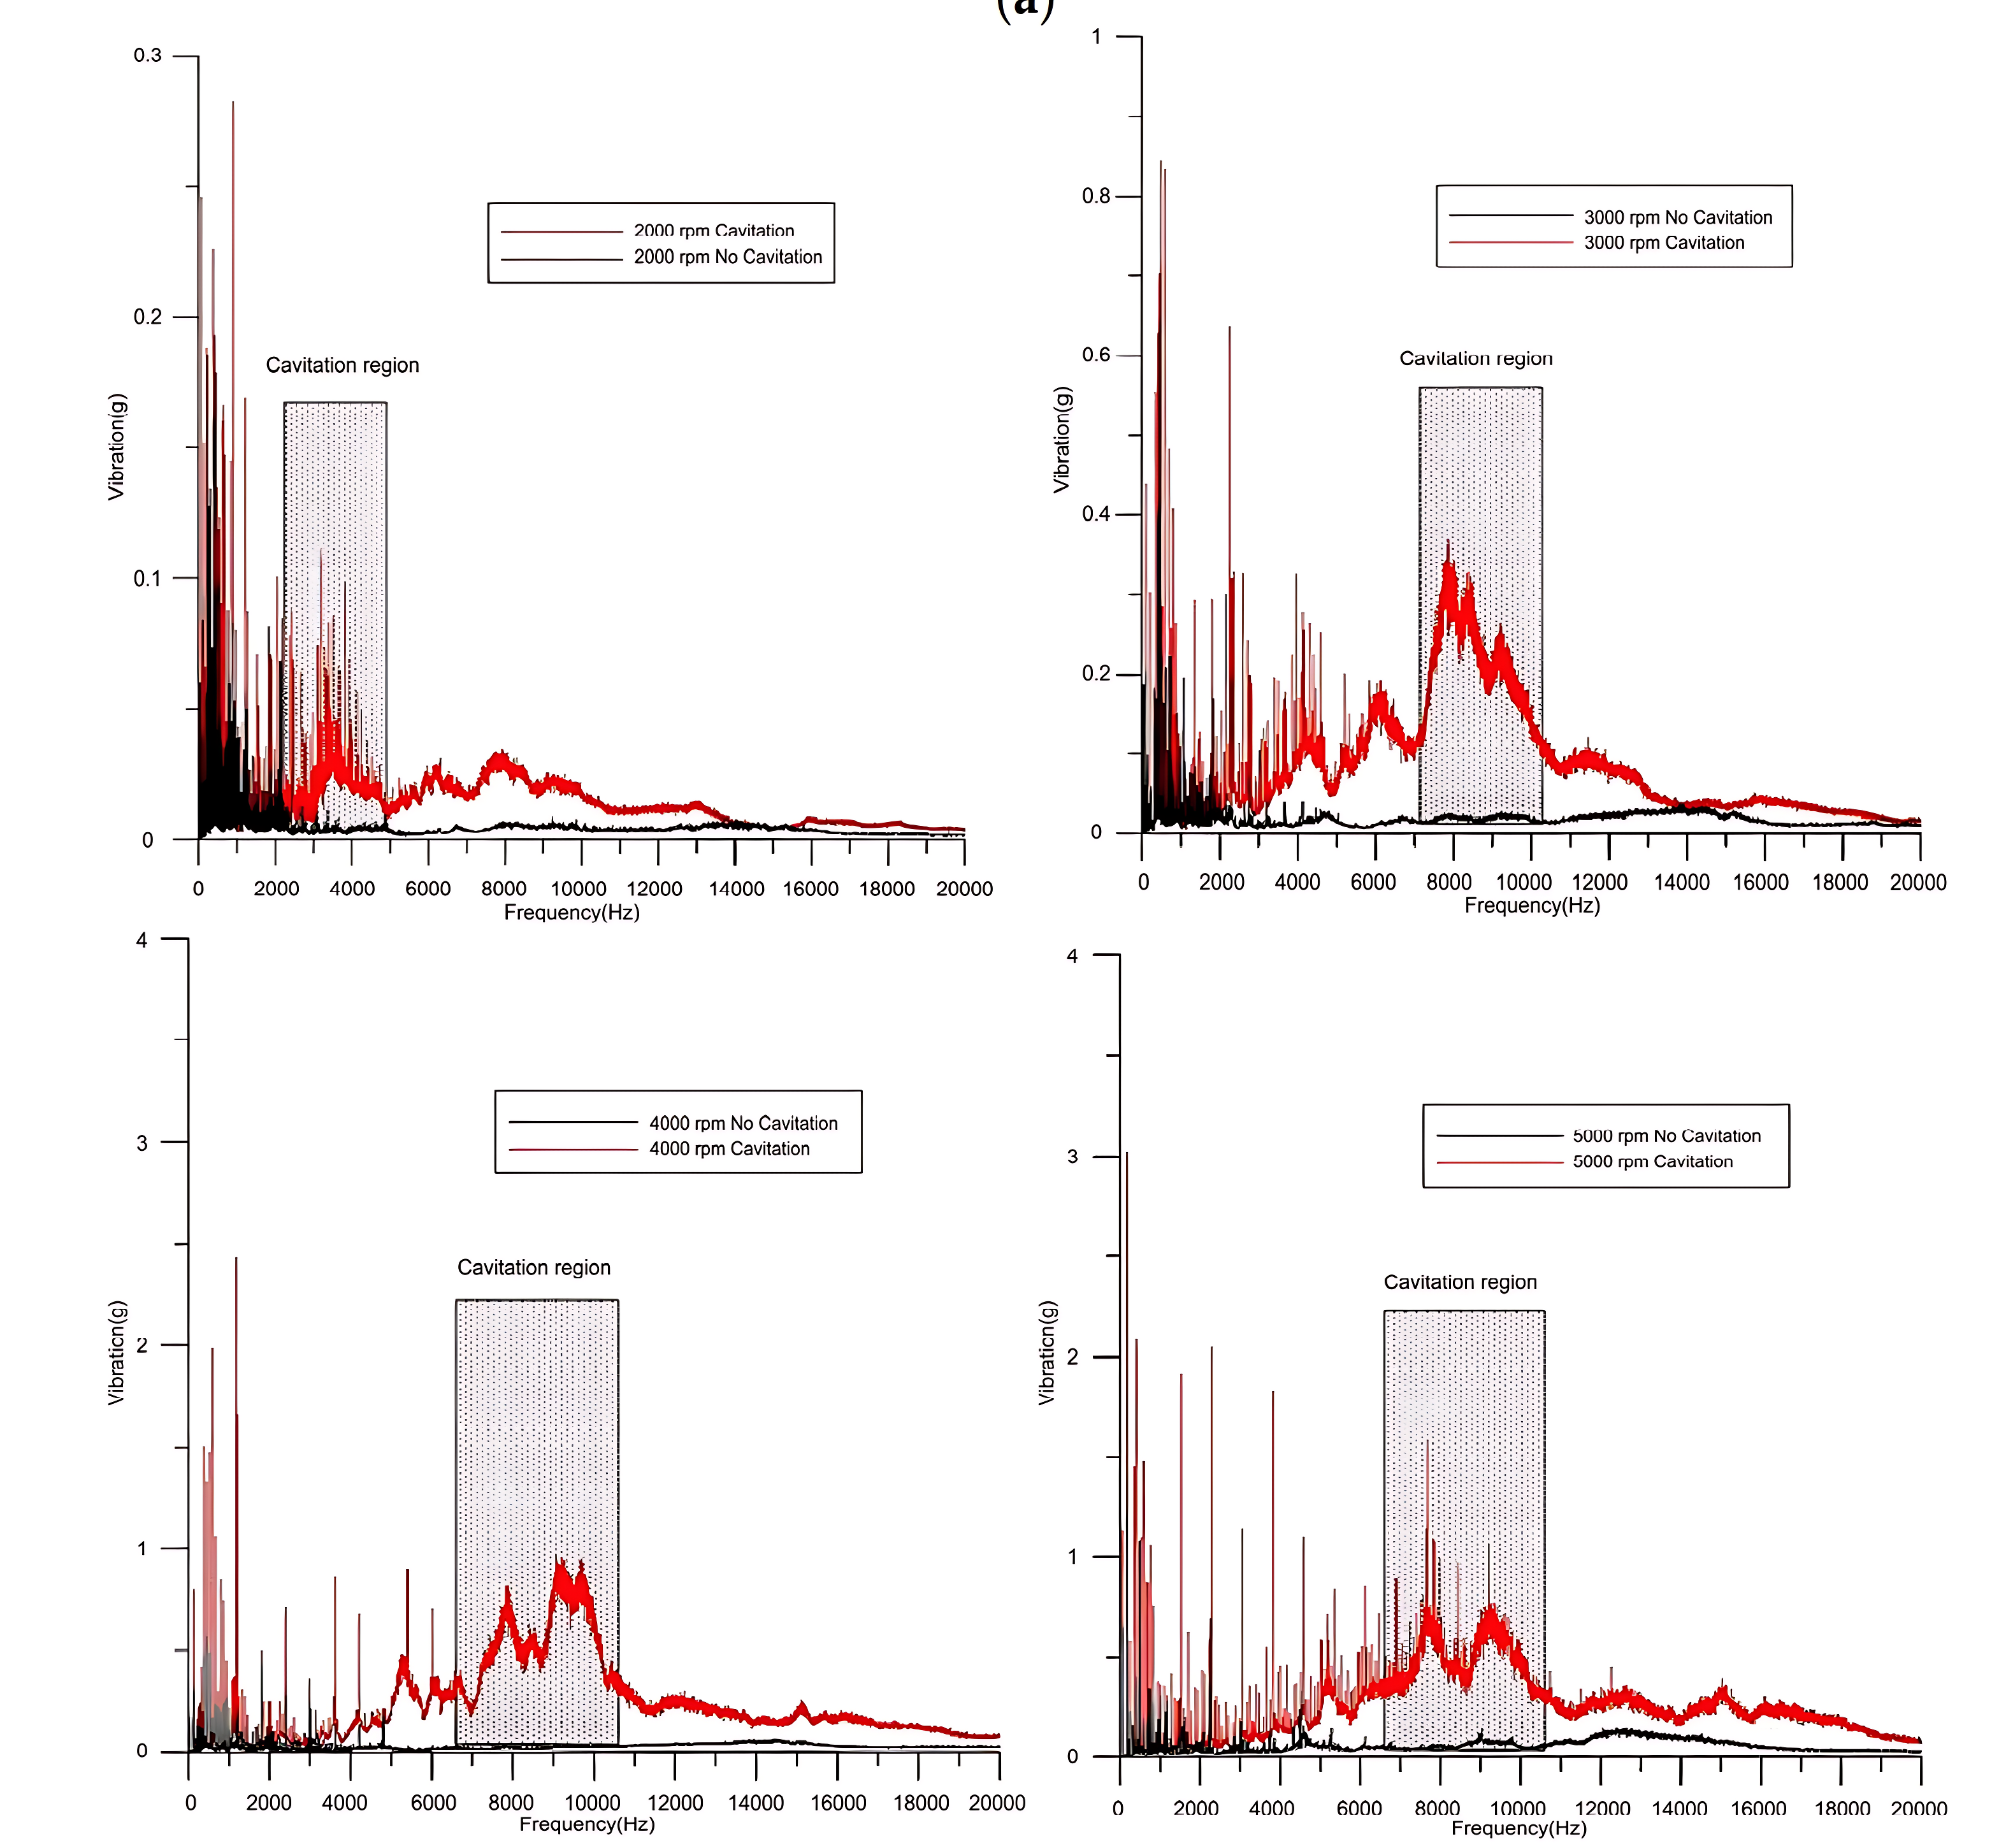
\includegraphics[width=0.95\linewidth]{figs//Artigos//Liu/Figura4B_Upscaler_4K.png}
    \caption{Espectro de sinal de vibração sob diferentes rpm. Fonte: \citeonline{liu2023review}}
    \label{fig:LiuFig4B}
\end{figure}

\linespread{1.27}\selectfont
Na Figura \ref{fig:LiuFig4B}, os sinais de vibração são analisados no domínio da frequência para diferentes velocidades de rotação (2000, 3000, 4000 e 5000 rpm). Os gráficos demonstram que, conforme a rotação aumenta, há um deslocamento e uma intensificação das componentes espectrais na faixa de 2 kHz a 8 kHz — região marcada como \textit{cavitation region}. Esses picos adicionais resultam da energia liberada pelos colapsos das bolhas de vapor, que introduzem novas componentes de alta frequência no espectro. A Figura \ref{fig:LiuFig4B} também mostra que a amplitude dessas componentes cresce com o aumento da rotação, evidenciando uma correlação direta entre a intensidade da cavitação e o conteúdo de alta frequência do sinal. Essa observação reforça a utilidade da análise espectral na \mbox{identificação e quantificação do fenômeno.}
\linespread{1.25}\selectfont

\begin{figure}[H]
    \centering
    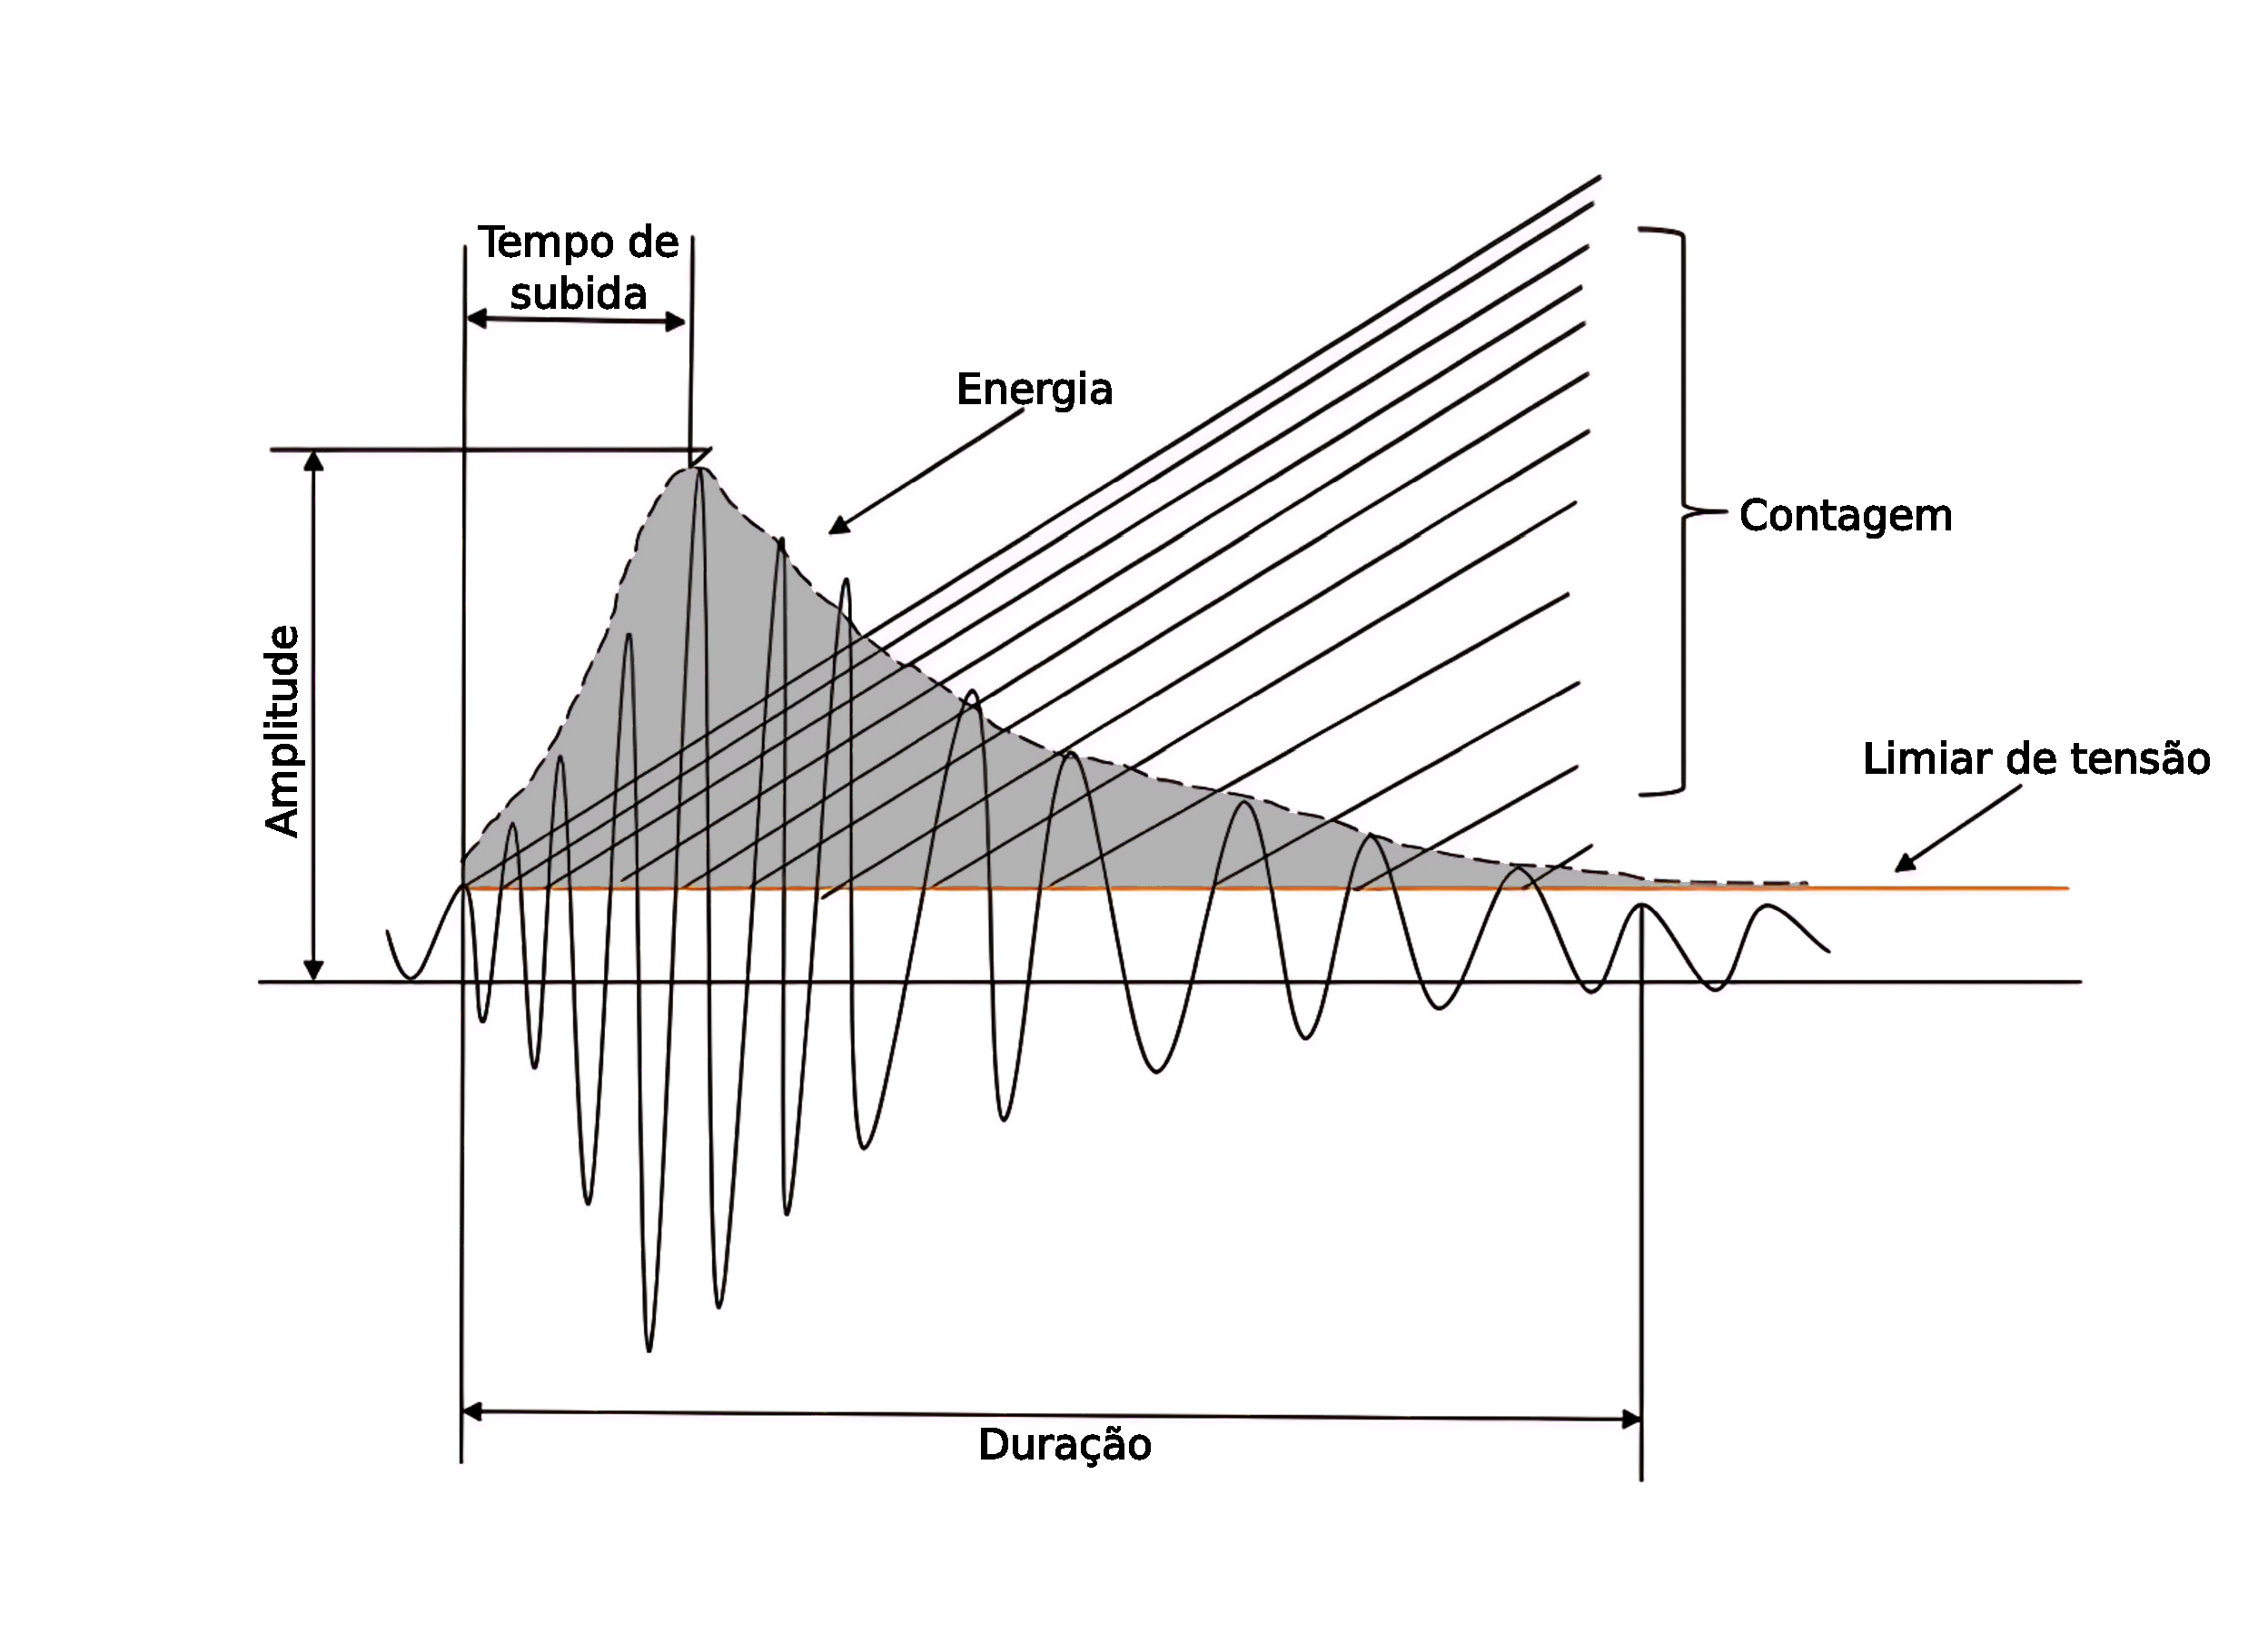
\includegraphics[width=0.9\linewidth]{figs//Artigos//Liu/Figura6.pdf}
    \caption{Parâmetros característicos do sinal de emissão acústica. Adaptado de  \citeonline{liu2023review}}
    \label{fig:LiuFig6}
\end{figure}

A Figura \ref{fig:LiuFig6} ilustra a decomposição de um evento típico de emissão acústica (“hit”) em seus principais parâmetros: amplitude, tempo de subida, \textit{rise time}, duração, energia e número de contagens acima do limiar, \textit{counts}. A amplitude representa o pico máximo do sinal, enquanto o tempo de subida corresponde ao intervalo entre o primeiro cruzamento do limiar e o pico máximo. A duração cobre o período total em que o sinal permanece acima do limiar, e a energia é obtida pela integral do sinal retificado. O número de contagens indica quantas vezes o sinal cruza o limiar estabelecido. Esses parâmetros são amplamente utilizados na caracterização de eventos de cavitação, pois refletem a intensidade e a frequência dos impactos associados ao colapso das bolhas, permitindo discriminar entre ruído e atividade cavitante real.

O ruído hidrodinâmico caracteriza-se por apresentar um espectro de banda larga e comportamento estocástico, resultante dos fenômenos de formação, crescimento e colapso de bolhas de vapor no interior do escoamento. Diferentemente do ruído mecânico, que tem natureza periódica e está associado a elementos estruturais da bomba (como mancais, rolamentos e pás do impulsor), o ruído hidrodinâmico reflete diretamente a instabilidade do fluido e as flutuações de pressão induzidas pela cavitação.

A Figura \ref{fig:LiuFig7}, adaptada de \citeonline{liu2023review}, apresenta a composição do ruído em bombas centrífugas, discriminando suas origens e mecanismos de formação. No topo, o ruído total da bomba, \textit{Pump noise} é dividido em dois grandes grupos: o ruído mecânico e o ruído hidrodinâmico. O primeiro engloba vibrações estruturais e ruídos discretos de frequência bem definida, como as frequências de passagem de pás e harmônicos, enquanto o segundo abrange componentes de ruído de cavitação, fluxo turbulento e separação de fluxo, de natureza predominantemente aleatória e de banda larga. Dentro do ruído de cavitação, por sua vez, distinguem-se componentes discretos e de banda larga, correspondentes a diferentes estágios e intensidades do fenômeno.

\begin{figure}[H]
\centering
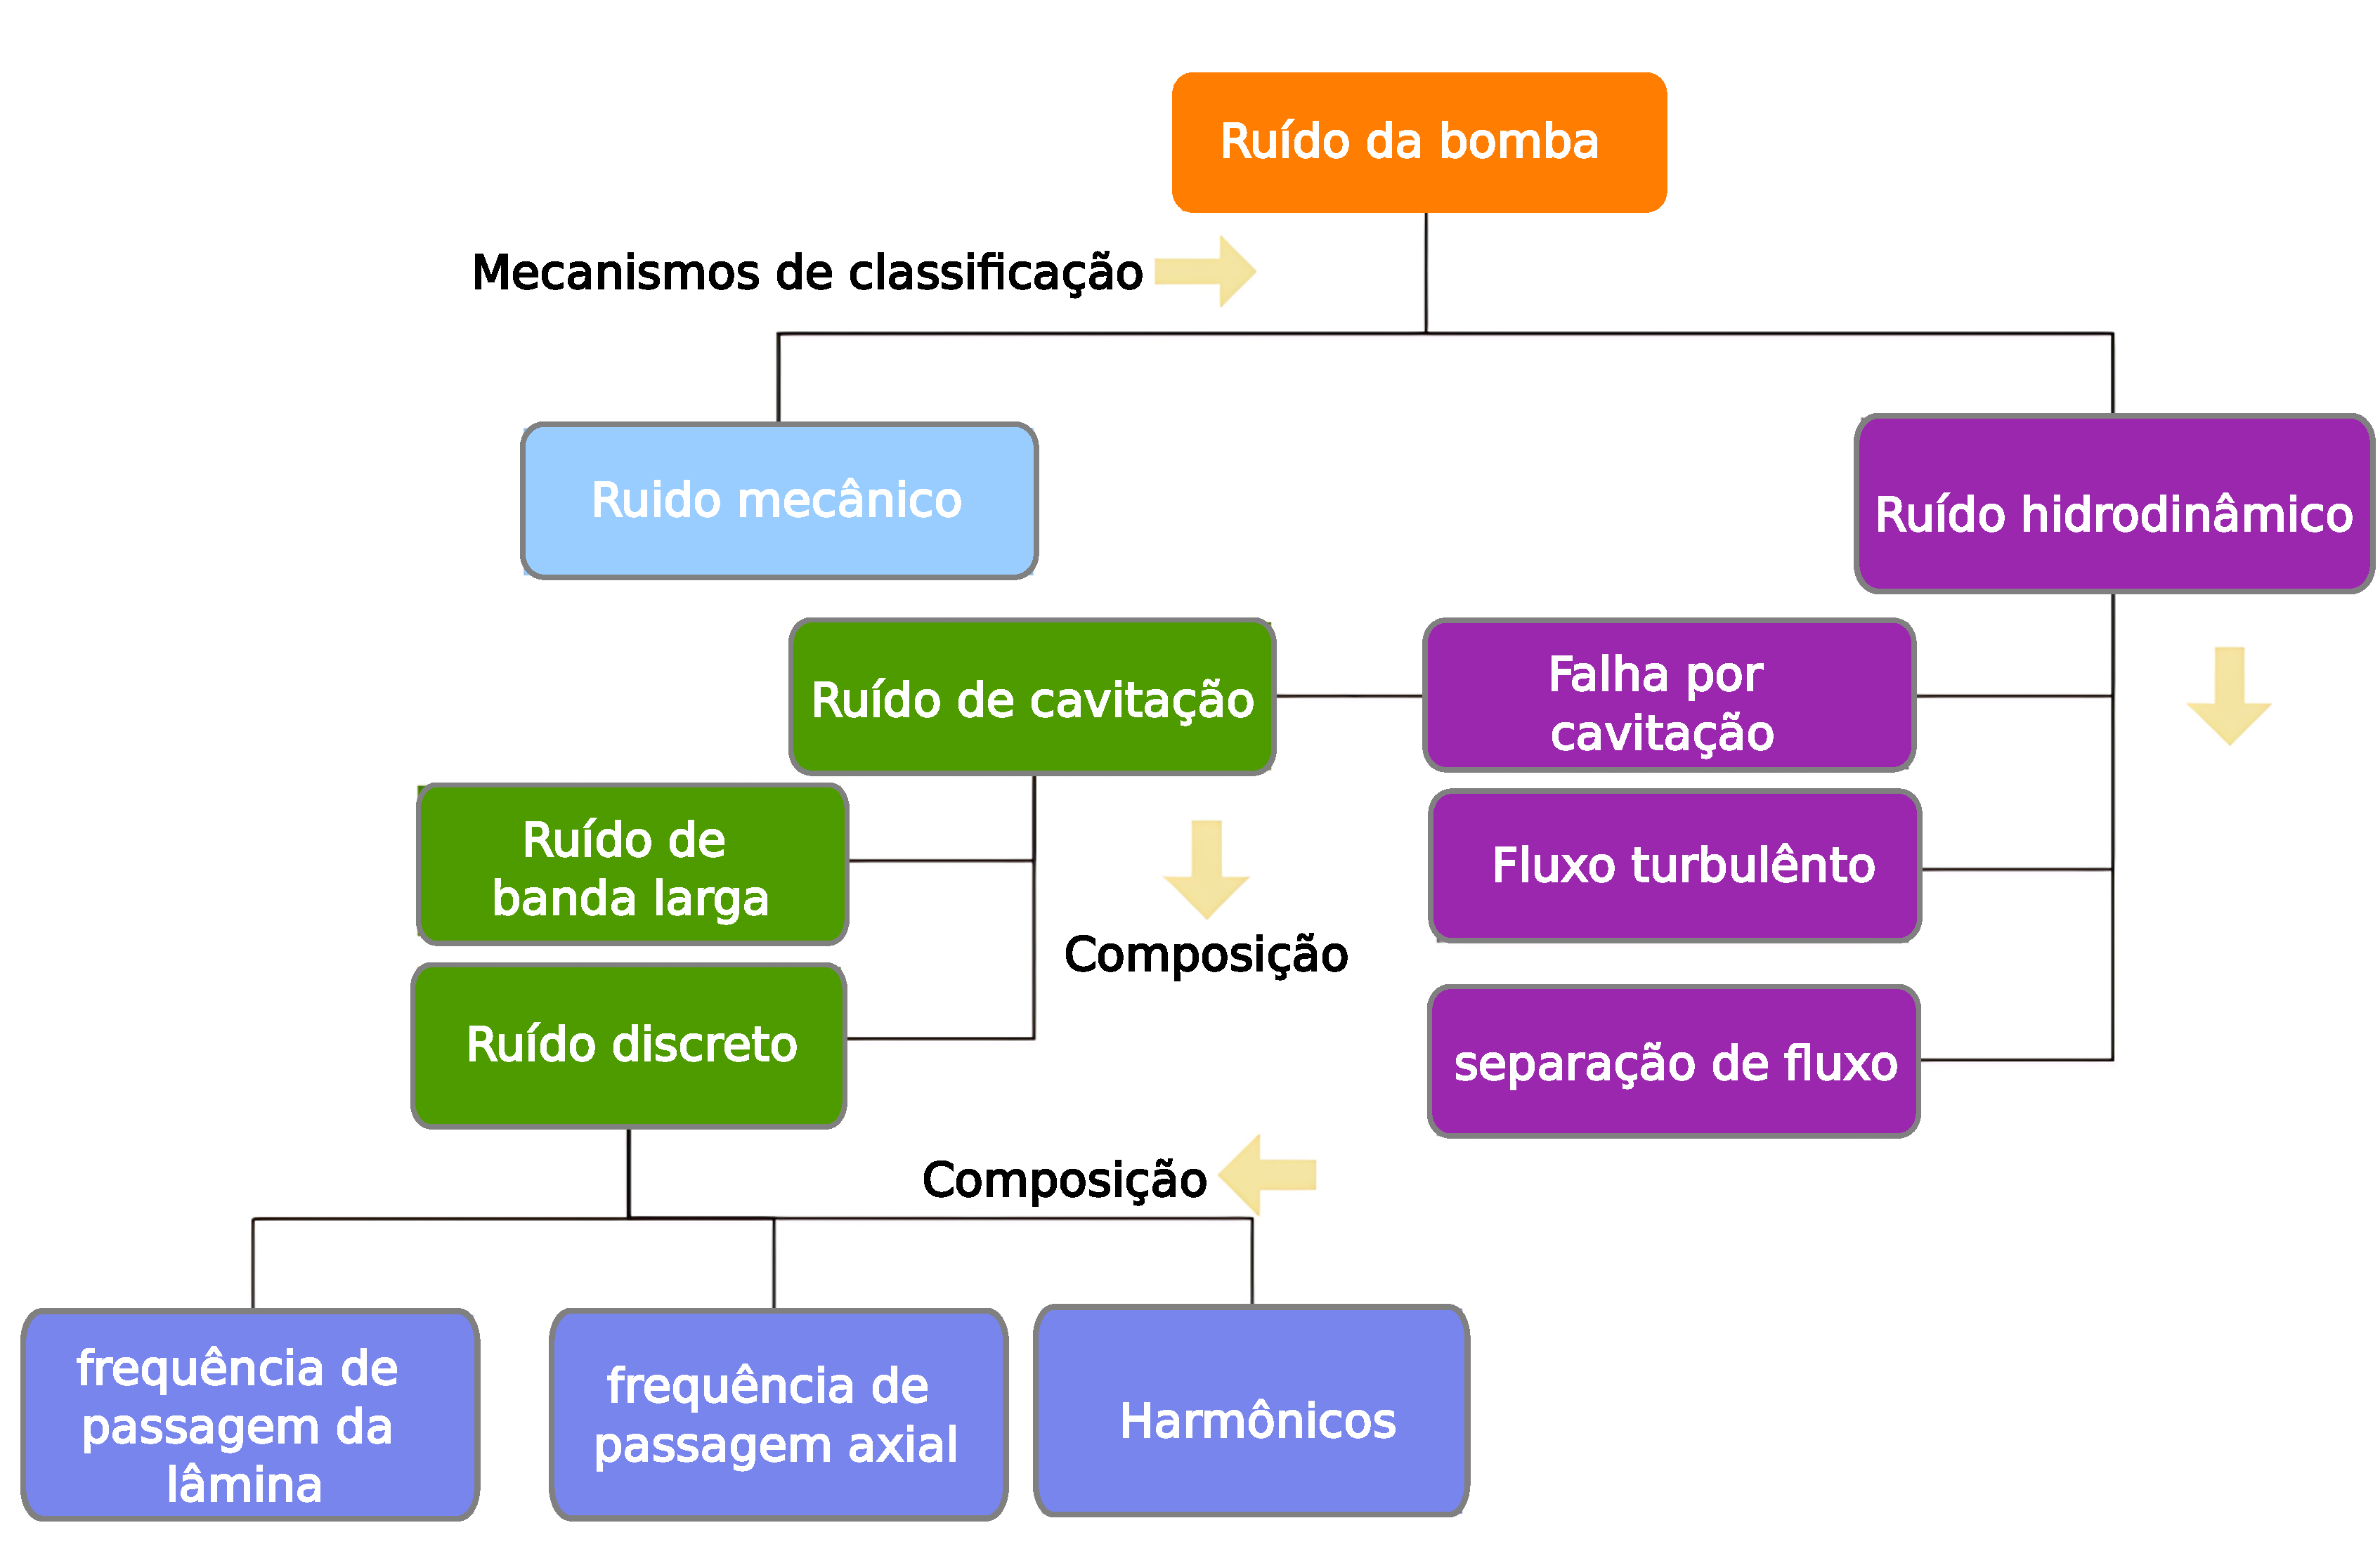
\includegraphics[width=0.75\linewidth]{figs//Artigos//Liu/Figura7.pdf}
\caption{Composição e mecanismos geradores do ruído em bombas centrífugas. Adaptado de \citeonline{liu2023review}.}
\label{fig:LiuFig7}
\end{figure}

Essa técnica de análise de ruído é particularmente útil em ensaios laboratoriais e ambientes controlados, nos quais as fontes de interferência externa podem ser minimizadas. Todavia, em aplicações industriais, sua eficácia tende a ser reduzida devido à forte influência de ruídos ambientais e à dificuldade de isolar as componentes específicas~associadas~à~cavitação.

Em contrapartida, o método baseado na pulsação de pressão apresenta maior robustez frente a interferências, uma vez que mede diretamente as variações de pressão no fluido, refletindo as flutuações hidráulicas e a eficiência volumétrica do sistema. Seu principal inconveniente, entretanto, é a natureza invasiva da instrumentação, que requer conexão física com o circuito hidráulico, além de uma baixa sensibilidade temporal para eventos de curta duração — o que limita sua capacidade de detectar a cavitação incipiente.

De modo comparativo, \citeonline{liu2023review} destacam que a emissão acústica e o ruído hidrodinâmico se sobressaem na detecção inicial da cavitação, enquanto a vibração é amplamente utilizada pela maturidade teórica e a pulsação de pressão pela robustez e simplicidade de implementação. As tendências futuras apontam para a convergência entre sensores de alta sensibilidade e métodos modernos de processamento de sinais não estacionários, aliada ao uso de inteligência artificial, em especial redes neurais convolucionais e aprendizado por reforço profundo, \mbox{para extração de padrões e detecção automatizada.}

Em síntese, a revisão conduzida por \citeonline{liu2023review} reforça que a emissão acústica permanece como uma das técnicas mais promissoras para a detecção precoce da cavitação, ainda que sua ampla adoção dependa de avanços em aspectos técnicos e econômicos, incluindo a redução de custos dos sensores piezoelétricos, a integração com hardware embarcado e o desenvolvimento de algoritmos otimizados para análise em tempo real.

\citeonline{poddar2021classification} apresentam um estudo voltado à detecção de falhas incipientes em mancais hidrodinâmicos, \textit{journal bearings}, investigando simultaneamente sinais EA e de vibração. Os autores ressaltam que fenômenos como cavitação, contaminação por partículas e falta de lubrificação são causas relevantes de degradação na performance de mancais, podendo levar à erosão, perda de eficiência e falhas prematuras. Neste contexto, métodos que permitam a identificação precoce dessas condições assumem papel crucial em estratégias de manutenção preditiva.

O experimento baseia-se em um arranjo monitorado, onde sensores de vibração e sensores de emissão acústica foram instalados em um mancal submetido a diferentes condições operacionais — incluindo variações no regime de carga, contaminação por partículas de diferentes tamanhos e situações de lubrificação insuficiente. O objetivo central consistiu em comparar a sensibilidade das duas técnicas, especialmente no que tange à detecção da cavitação incipiente. Os sinais coletados foram processados nos domínios do tempo e da frequência, a partir dos quais foram extraídos parâmetros como RMS, fator de crista, amplitude de pico, energia acumulada e número de contagens (no caso da EA). A análise foi estendida ao domínio tempo-frequência para capturar a \mbox{evolução espectral dos fenômenos de falha.}

Os resultados demonstram que os sinais de vibração apresentaram alterações significativas apenas em estágios mais avançados dos defeitos, quando ocorreram instabilidades acusadas no escoamento ou deterioração clara da película hidráulica. Em contraste, os sinais de emissão acústica revelaram-se muito mais sensíveis em estágios iniciais; observou-se, por exemplo, crescimento progressivo dos parâmetros energia acumulada e número de contagens com o agravamento da condição, o que evidencia uma correlação direta com os eventos de colapso de bolhas ou microcontatos. Os autores também apontam que amplitude e largura de banda dos sinais EA expandem-se de modo notável sob condições de falha — enquanto os índices de vibração \mbox{mantêm-se relativamente estáveis.}

A discussão conclui que a técnica de emissão acústica apresenta desempenho claramente superior na detecção precoce da cavitação e de deteriorações relacionadas, pois consegue identificar alterações no regime de escoamento antes mesmo que se verifique qualquer impacto mensurável no desempenho hidrodinâmico global do equipamento. A análise vibracional, embora útil, tende a ser mais responsiva em estágios posteriores da falha, quando modificações estruturais ou oscilações adicionais já se refletem na resposta dinâmica do conjunto. Do ponto de vista metodológico, o estudo indica que a integração entre ambas as abordagens pode enriquecer o diagnóstico, ampliando a compreensão do processo de degradação. Contudo, mesmo sem recorrer a medições complementares, a EA já se mostra como a alternativa mais sensível e promissora para a identificação incipiente de cavitação, conforme evidenciado em \citeonline{poddar2021classification}.

\citeonline{amini2022development} apresentam o desenvolvimento de um sistema inovador para o monitoramento da cavitação em turbinas hidráulicas, fundamentado na análise de sinais acústicos aliada a algoritmos de aprendizado de máquina. Os autores apontam que a operação de turbinas em condições fora do ponto ótimo de eficiência aumenta a probabilidade de ocorrência de cavitação, o que por sua vez acarreta degradação de desempenho, vibrações estruturais e, principalmente, danos mecânicos por erosão. Nesse sentido, a proposta busca oferecer uma ferramenta não intrusiva, capaz de detectar tanto a ocorrência quanto a severidade do fenômeno em tempo real, contribuindo para a manutenção preditiva em centrais hidrelétricas.

A metodologia foi organizada em duas fases distintas. Na primeira, foram realizados experimentos controlados no túnel de cavitação da HES-SO Valais/Wallis, em que se utilizou um hidrofólio de aço inoxidável do tipo NACA 0015 para induzir a cavitação em condições estáticas e dinâmicas, conforme ilustrado na Figura \ref{fig:amini2022developmentFig1}. Nessa etapa, o ruído no aerofólio foi registrado por meio de um microfone GRAS 46 AE com frequência de amostragem de 40 kHz, e os sinais foram analisados nos domínios temporal e espectral. Em uma segunda fase, a técnica foi validada em escala real na usina hidrelétrica de Ernen, no cantão de Valais (Suíça), equipada com turbinas Francis de 16 MW cada, como mostra a Figura \ref{fig:amini2022developmentFig2}. Durante essa campanha experimental, foram simuladas diferentes condições operacionais, abrangendo variações de carga, níveis de jusante e introdução de ruídos artificiais, com o intuito de avaliar a robustez do sistema.

\begin{figure}[H]
    \centering
    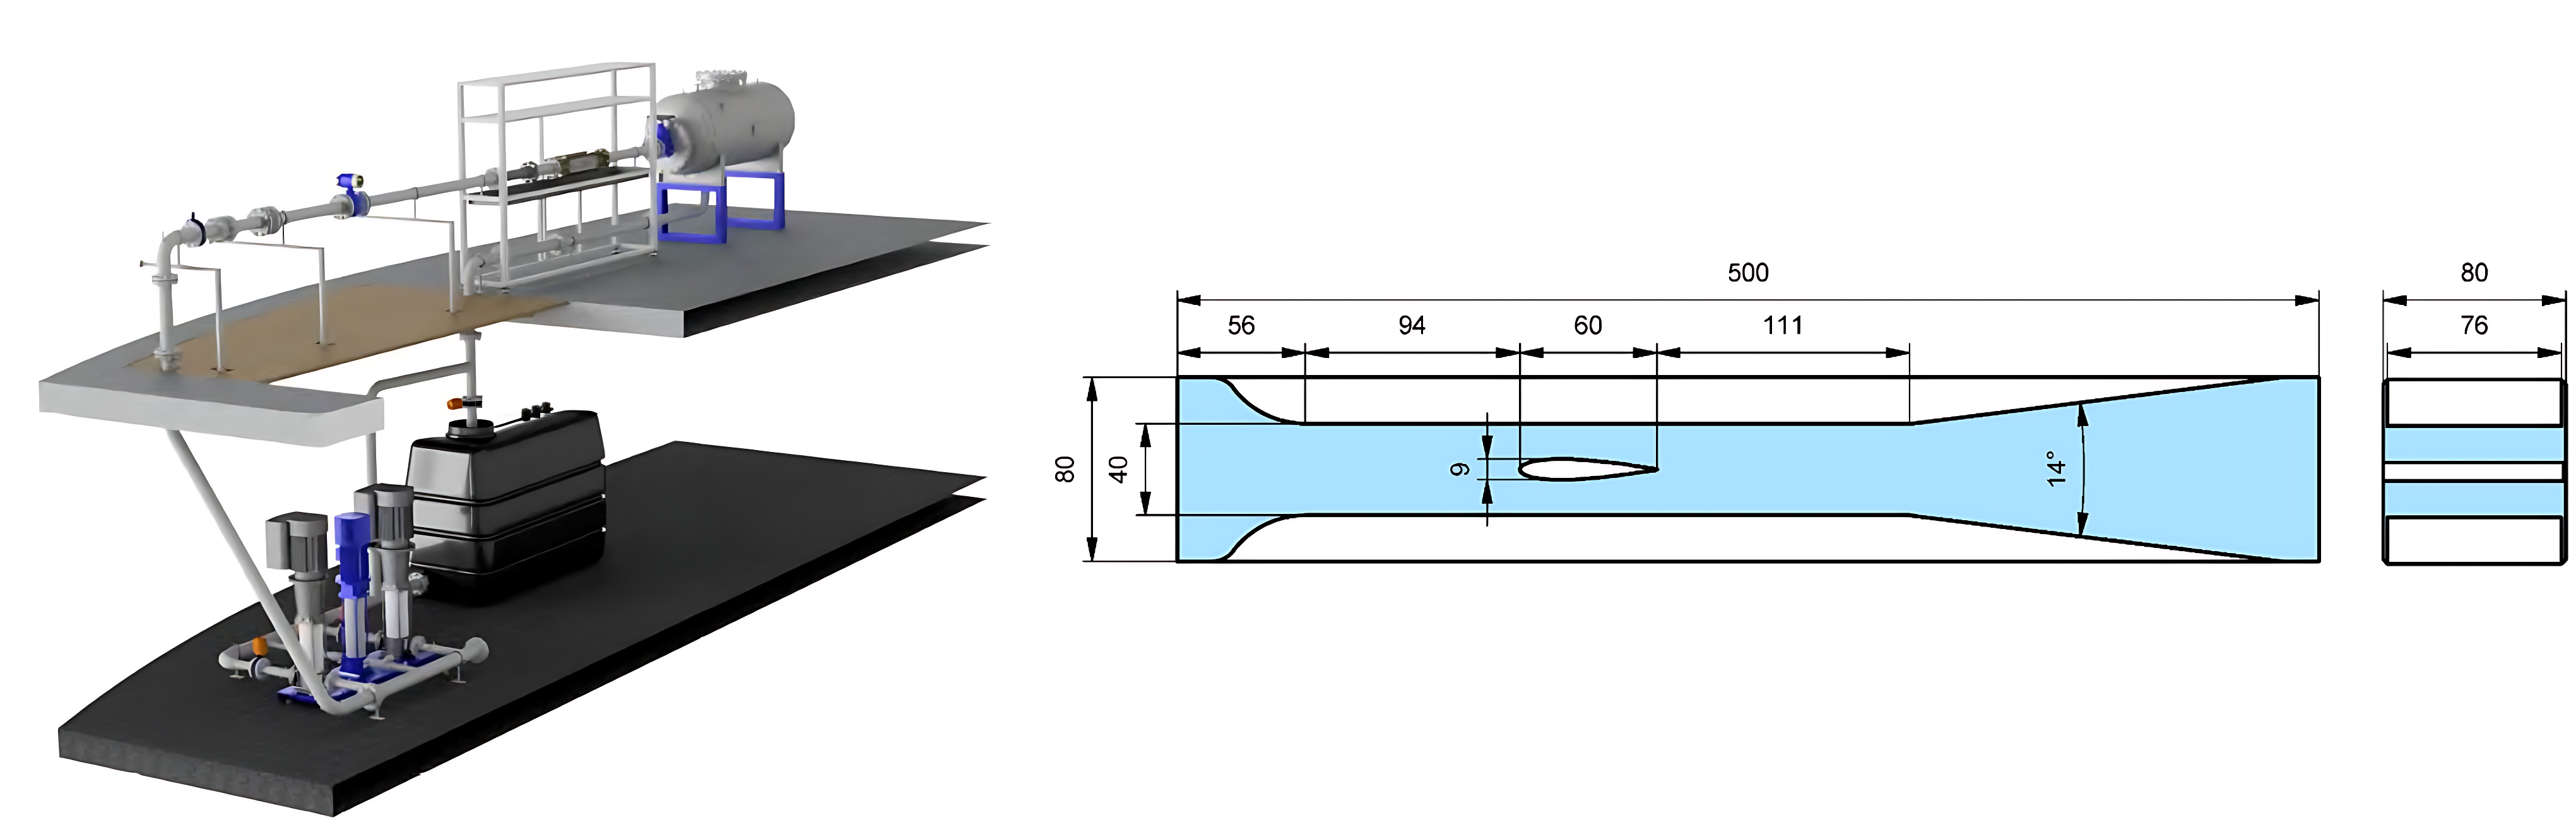
\includegraphics[width=1.0\linewidth]{figs/Artigos/amini2022development/Figura1_Upscaler_2K.png}
    \caption{(À esquerda) esquema do túnel de cavitação da HES-SO Valais/Wallis; (À direita) seção transversal do hidrofólio de aço inoxidável NACA 0015 testado. Fonte: \citeonline{amini2022development}}
    \label{fig:amini2022developmentFig1}
\end{figure}

\begin{figure}[H]
    \centering
    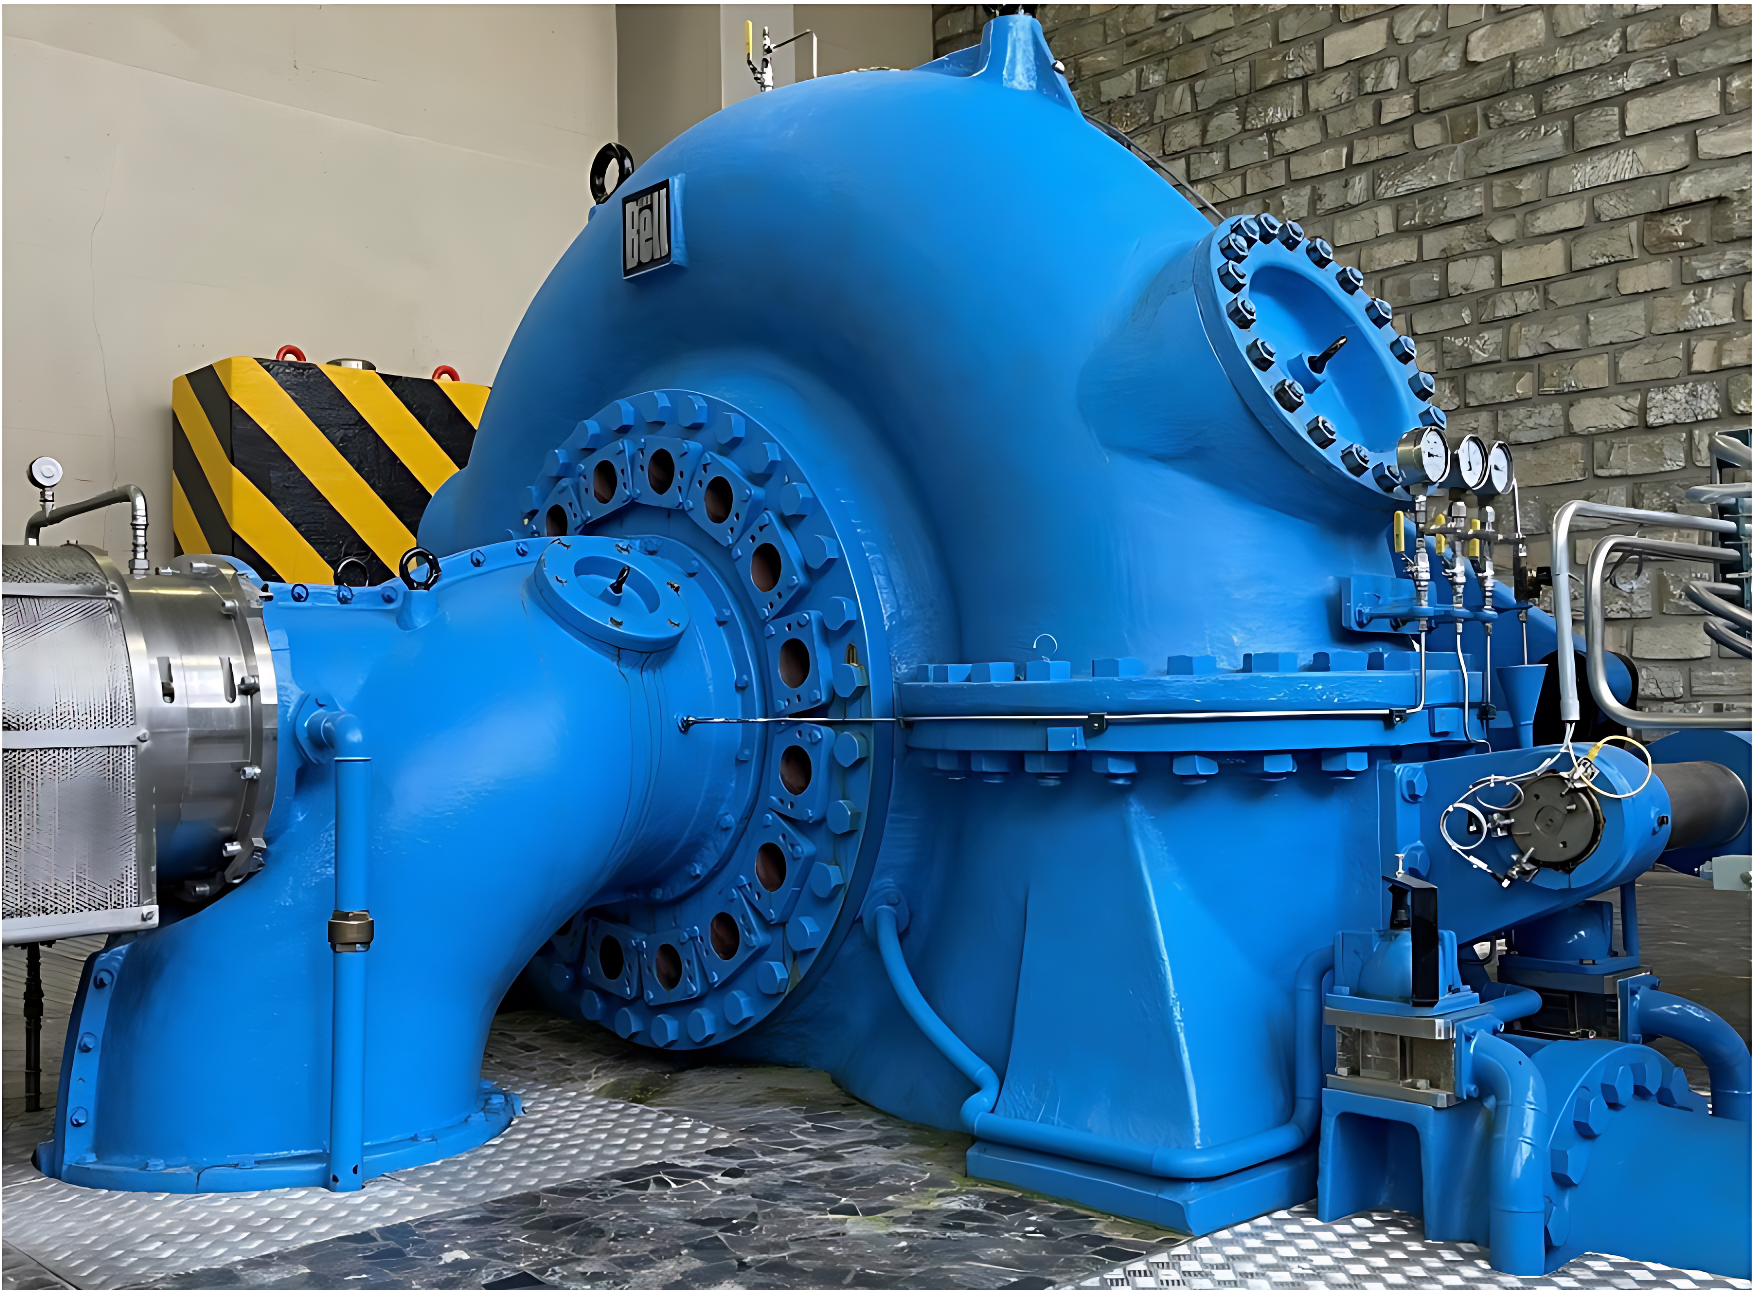
\includegraphics[width=.85\linewidth]{figs/Artigos/amini2022development/Figura2_Upscaler_2K.png}
    \caption{Turbina Francis de dois rotores na usina hidrelétrica de Ernen (Wallis, Suíça). Fonte: \citeonline{amini2022development}}
    \label{fig:amini2022developmentFig2}
\end{figure}

\linespread{1.27}\selectfont
As figuras explicam por si o salto metodológico:  
Figura \ref{fig:amini2022developmentFig1}: ilustra a instalação experimental de bancada no túnel de cavitação, onde o hidrofólio NACA 0015 foi submetido a perfis de escoamento com pressão de sucção reduzida para induzir cavitação. O desenho da seção transversal do hidrofólio permite visualizar as dimensões e geometria usadas nos testes. Essa figura demonstra claramente a etapa de laboratório, onde as condições são controladas, permitindo análise precisa dos sinais acústicos captados.

Figura \ref{fig:amini2022developmentFig2}: apresenta a aplicação em campo real, com uma turbina Francis de dois rotores na usina de Ernen. Essa imagem reforça a transição da metodologia do laboratório para o ambiente operacional industrial, destacando a compatibilidade da solução desenvolvida com sistemas de grande escala. A capacidade de validação em usina real confere maior credibilidade à técnica proposta.  

Em resumo, o estudo reforça a viabilidade do uso de sinais acústicos não invasivos em combinação com algoritmos de aprendizado para o monitoramento da cavitação em turbinas hidráulicas. A abordagem — centrada em microfones, processamento de sinais e classificação supervisionada — fornece uma estrutura promissora para aplicações industriais, o que dialoga diretamente com o foco desta dissertação: a implementação simulada de uma rede neural de convolução (CNN-1D) em hardware reconfigurável (FPGA) para detecção de falhas em sistemas hidráulicos.

\linespread{1.27}\selectfont
O processamento dos sinais foi realizado por meio da transformada rápida de Fourier (FFT) e da extração de características no domínio da frequência, com o objetivo de identificar padrões representativos da cavitação. Para a etapa de classificação supervisionada, foram testados dois algoritmos de aprendizado de máquina: o \textit{k-Nearest Neighbors} (k-NN), aplicado aos ensaios laboratoriais, e o \textit{Gaussian Mixture Model} (GMM), utilizado para os dados coletados na usina. 

Os resultados mostraram que, em condições estáticas de laboratório, a distinção entre regimes cavitantes e não cavitantes foi clara, atingindo 100\% de acurácia. Já nos ensaios dinâmicos, a precisão manteve-se elevada, superior a 95\%, mesmo diante da maior complexidade imposta pela rotulagem de dados e pela ausência de critérios visuais diretos para validação, como ilustram as Figuras~\ref{fig:amini2022developmentFig3} e~\ref{fig:amini2022developmentFig4}. Na aplicação em escala real, apesar da presença de ruído de fundo significativo, o algoritmo manteve desempenho consistente, separando com clareza as diferentes classes de operação e identificando distintos níveis de severidade da cavitação, conforme apresentado na Figura~\ref{fig:amini2022developmentFig6}.

\begin{figure}[H]
    \centering
    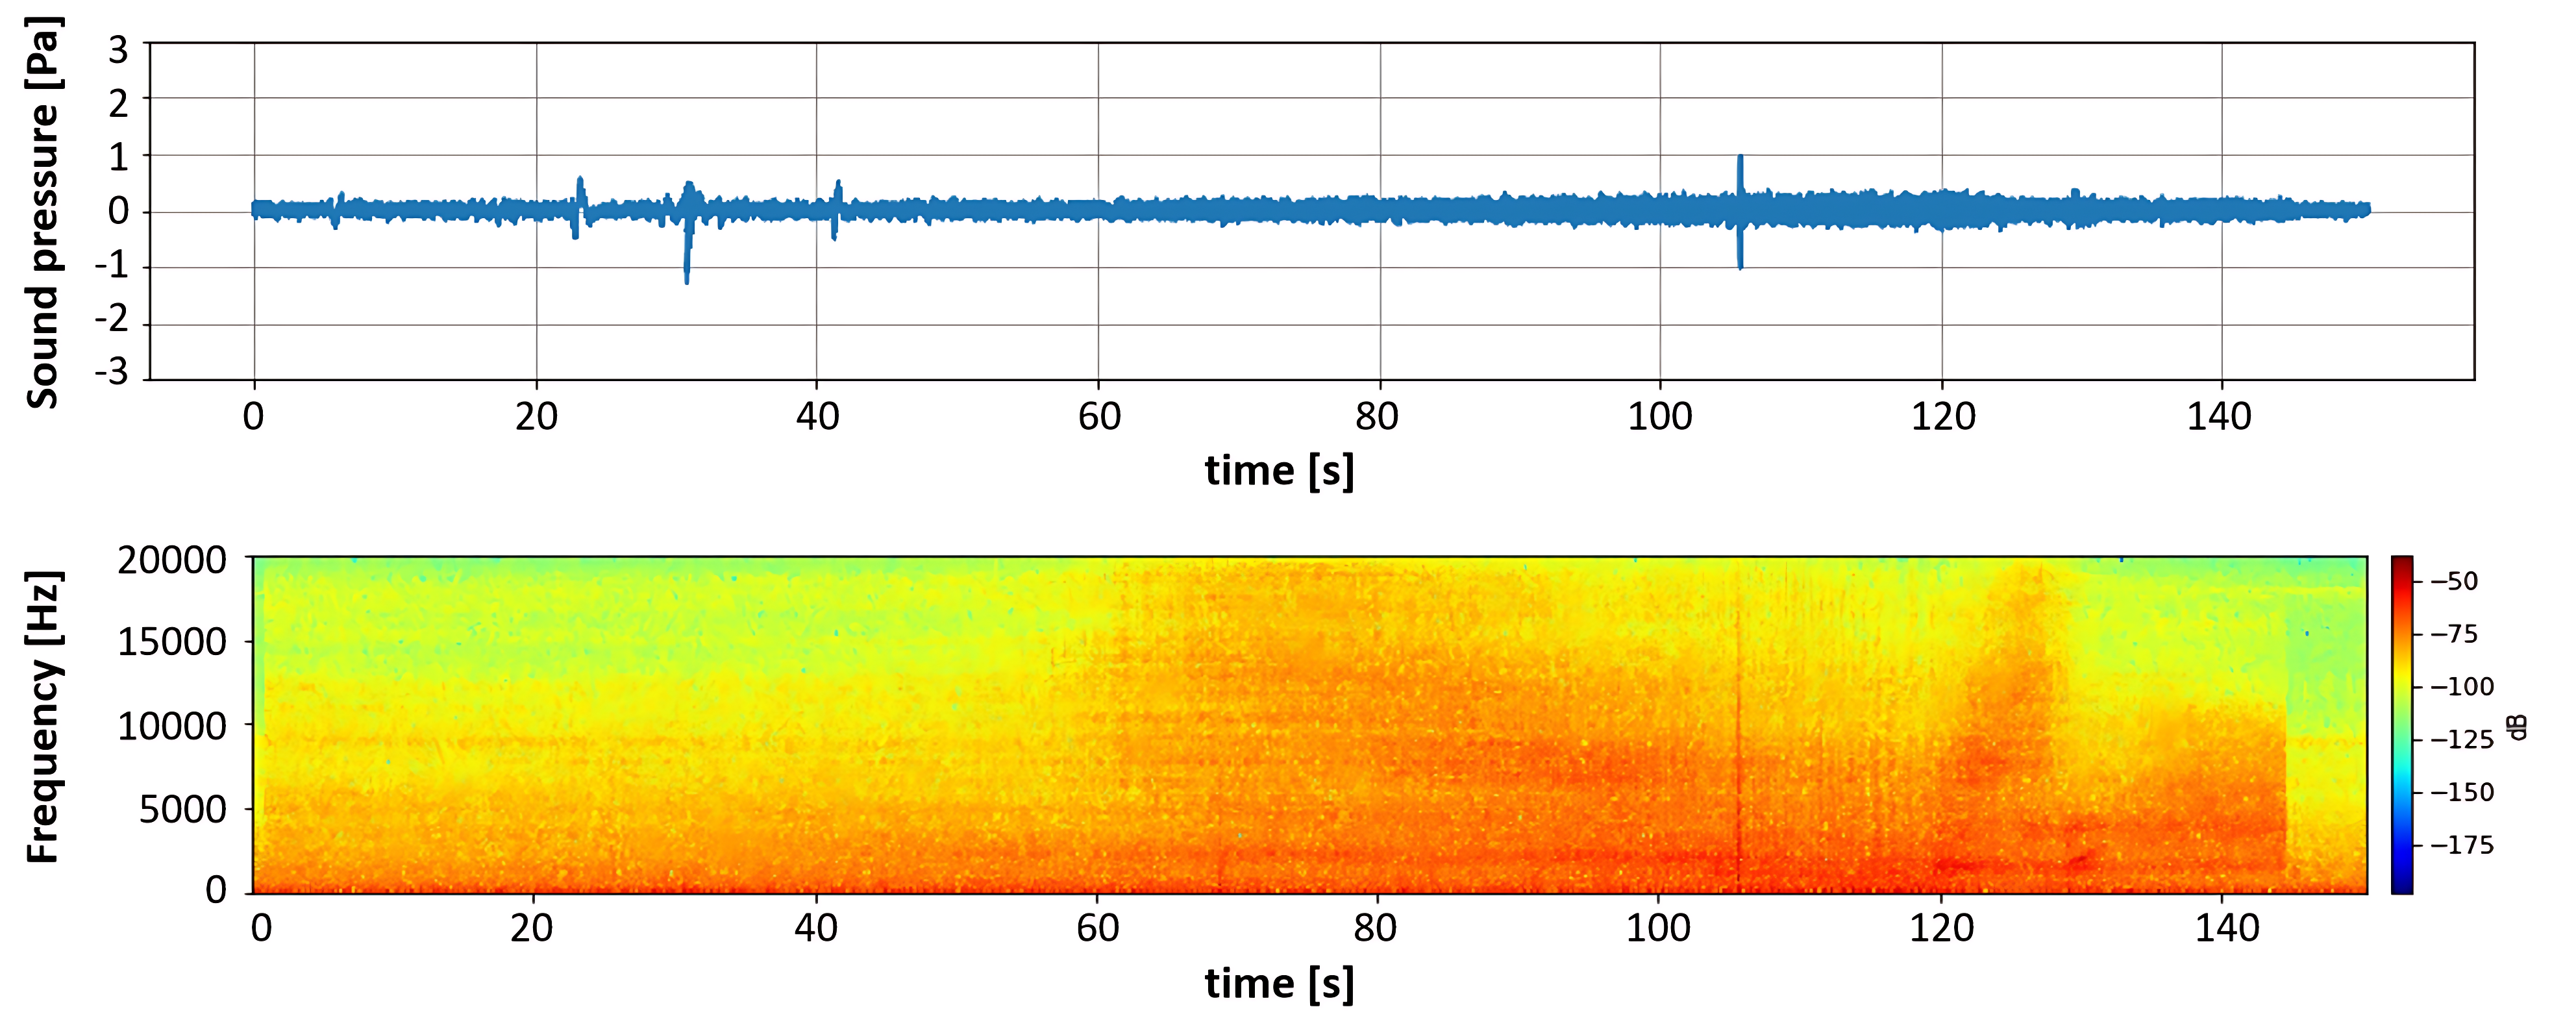
\includegraphics[width=1.0\linewidth]{figs/Artigos/amini2022development/Figura3_Upscaler_2K.png}
    \caption{Sinal acústico de um teste dinâmico ilustrado nos domínios de tempo (acima) e de frequência (abaixo). Fonte: \citeonline{amini2022development}}
    \label{fig:amini2022developmentFig3}
\end{figure}

\linespread{1.27}\selectfont
A Figura~\ref{fig:amini2022developmentFig3} apresenta o sinal acústico registrado durante um teste dinâmico. A parte superior mostra a variação da pressão sonora no tempo, enquanto o espectrograma inferior exibe a distribuição de energia no domínio da frequência. É possível observar o aumento de componentes de alta frequência à medida que a cavitação se intensifica, evidenciando a sensibilidade do método acústico.
\linespread{1.25}\selectfont

\begin{figure}[H]
    \centering
    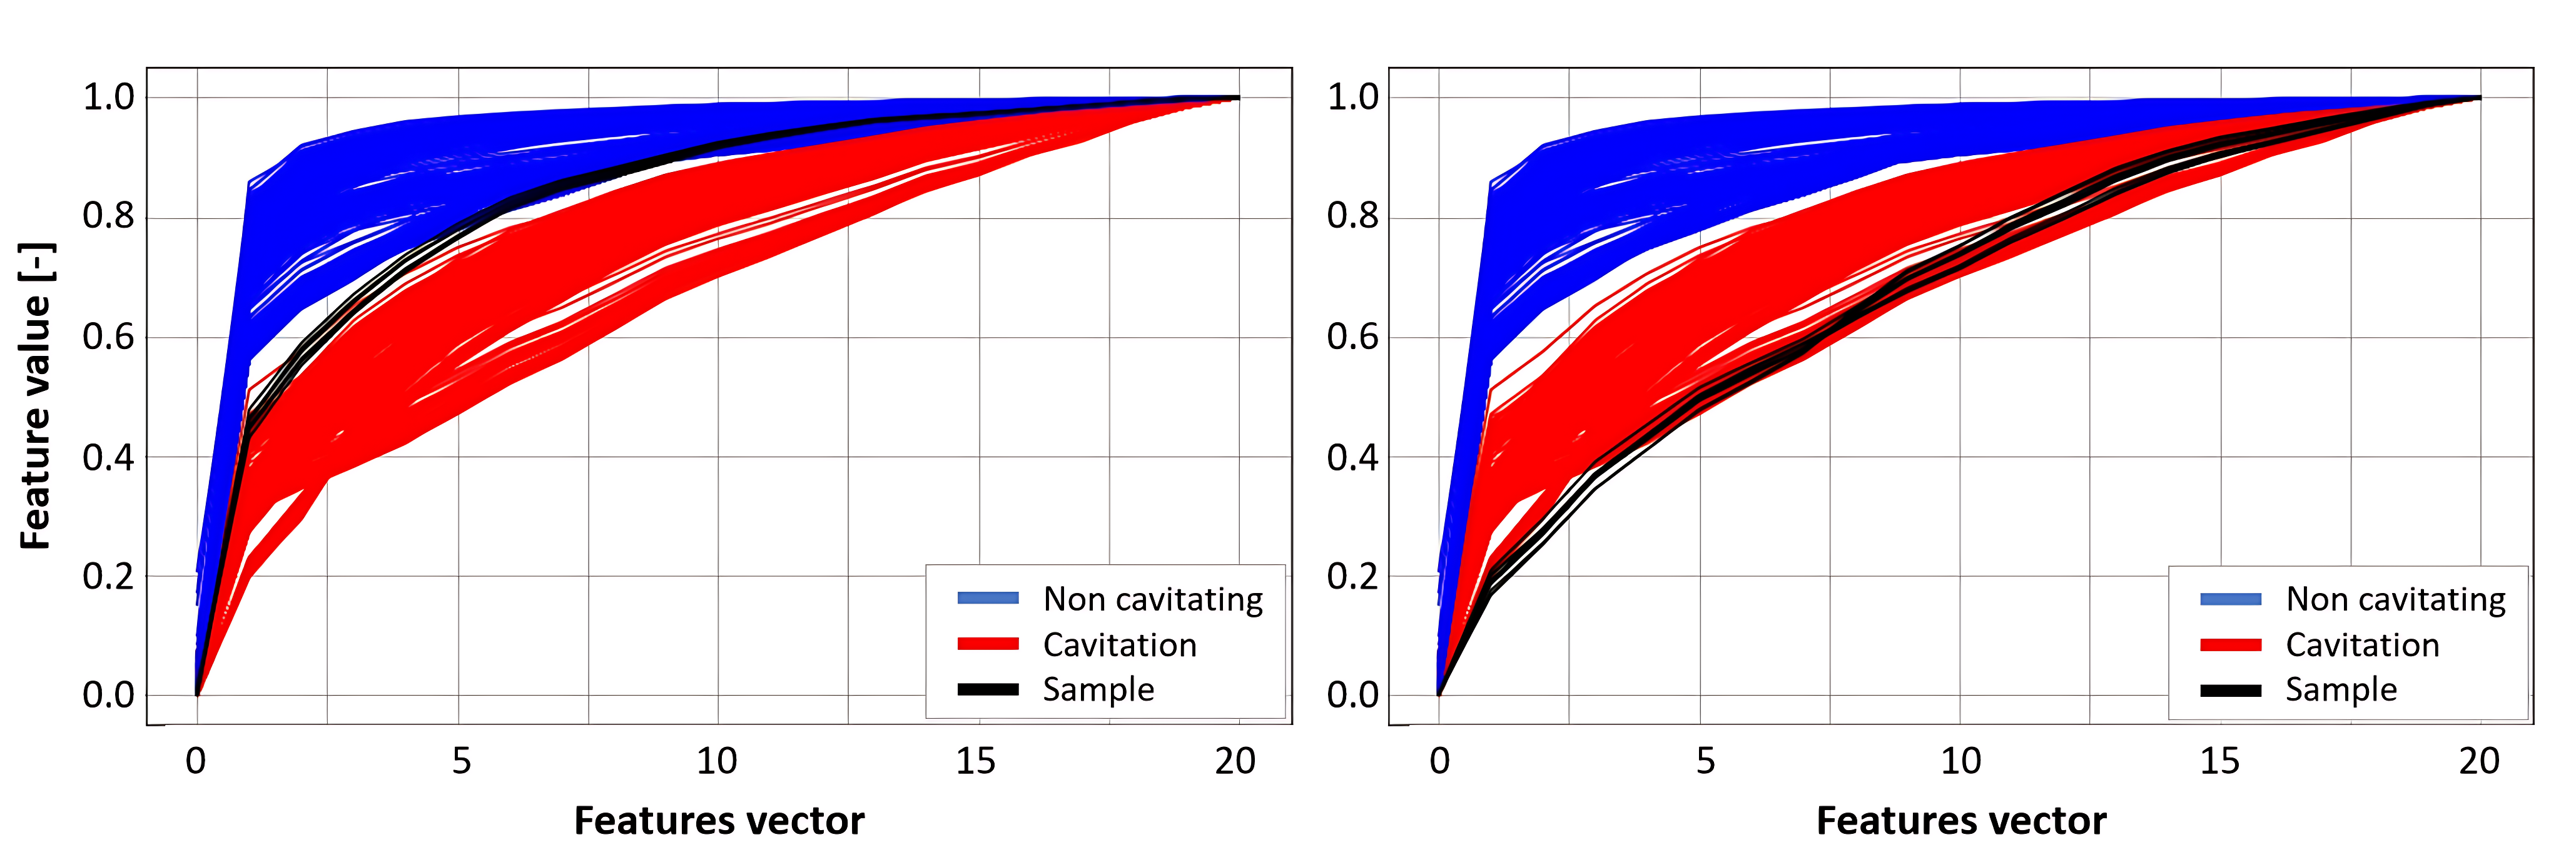
\includegraphics[width=1.0\linewidth]{figs/Artigos/amini2022development/Figura4_Upscaler_2K.png}
    \caption{Distribuição dos valores característicos extraídos dos sinais de ML para fluxos cavitantes (vermelho) e não cavitantes (azul), obtidos em testes estáticos com $\alpha = 8^\circ$. A curva preta à esquerda corresponde ao estado não cavitante em um teste dinâmico no mesmo ângulo, enquanto a curva à direita representa a condição cavitante sob o mesmo regime. Fonte: \citeonline{amini2022development}}
    \label{fig:amini2022developmentFig4}
\end{figure}

A Figura~\ref{fig:amini2022developmentFig4} mostra a distribuição das características extraídas dos sinais para diferentes condições de escoamento. Os fluxos cavitantes apresentam valores de atributos significativamente distintos dos não cavitantes, permitindo uma separação clara entre as classes. As curvas pretas destacam um teste dinâmico intermediário, demonstrando coerência entre as transições de regime.

\begin{figure}[H]
    \centering
    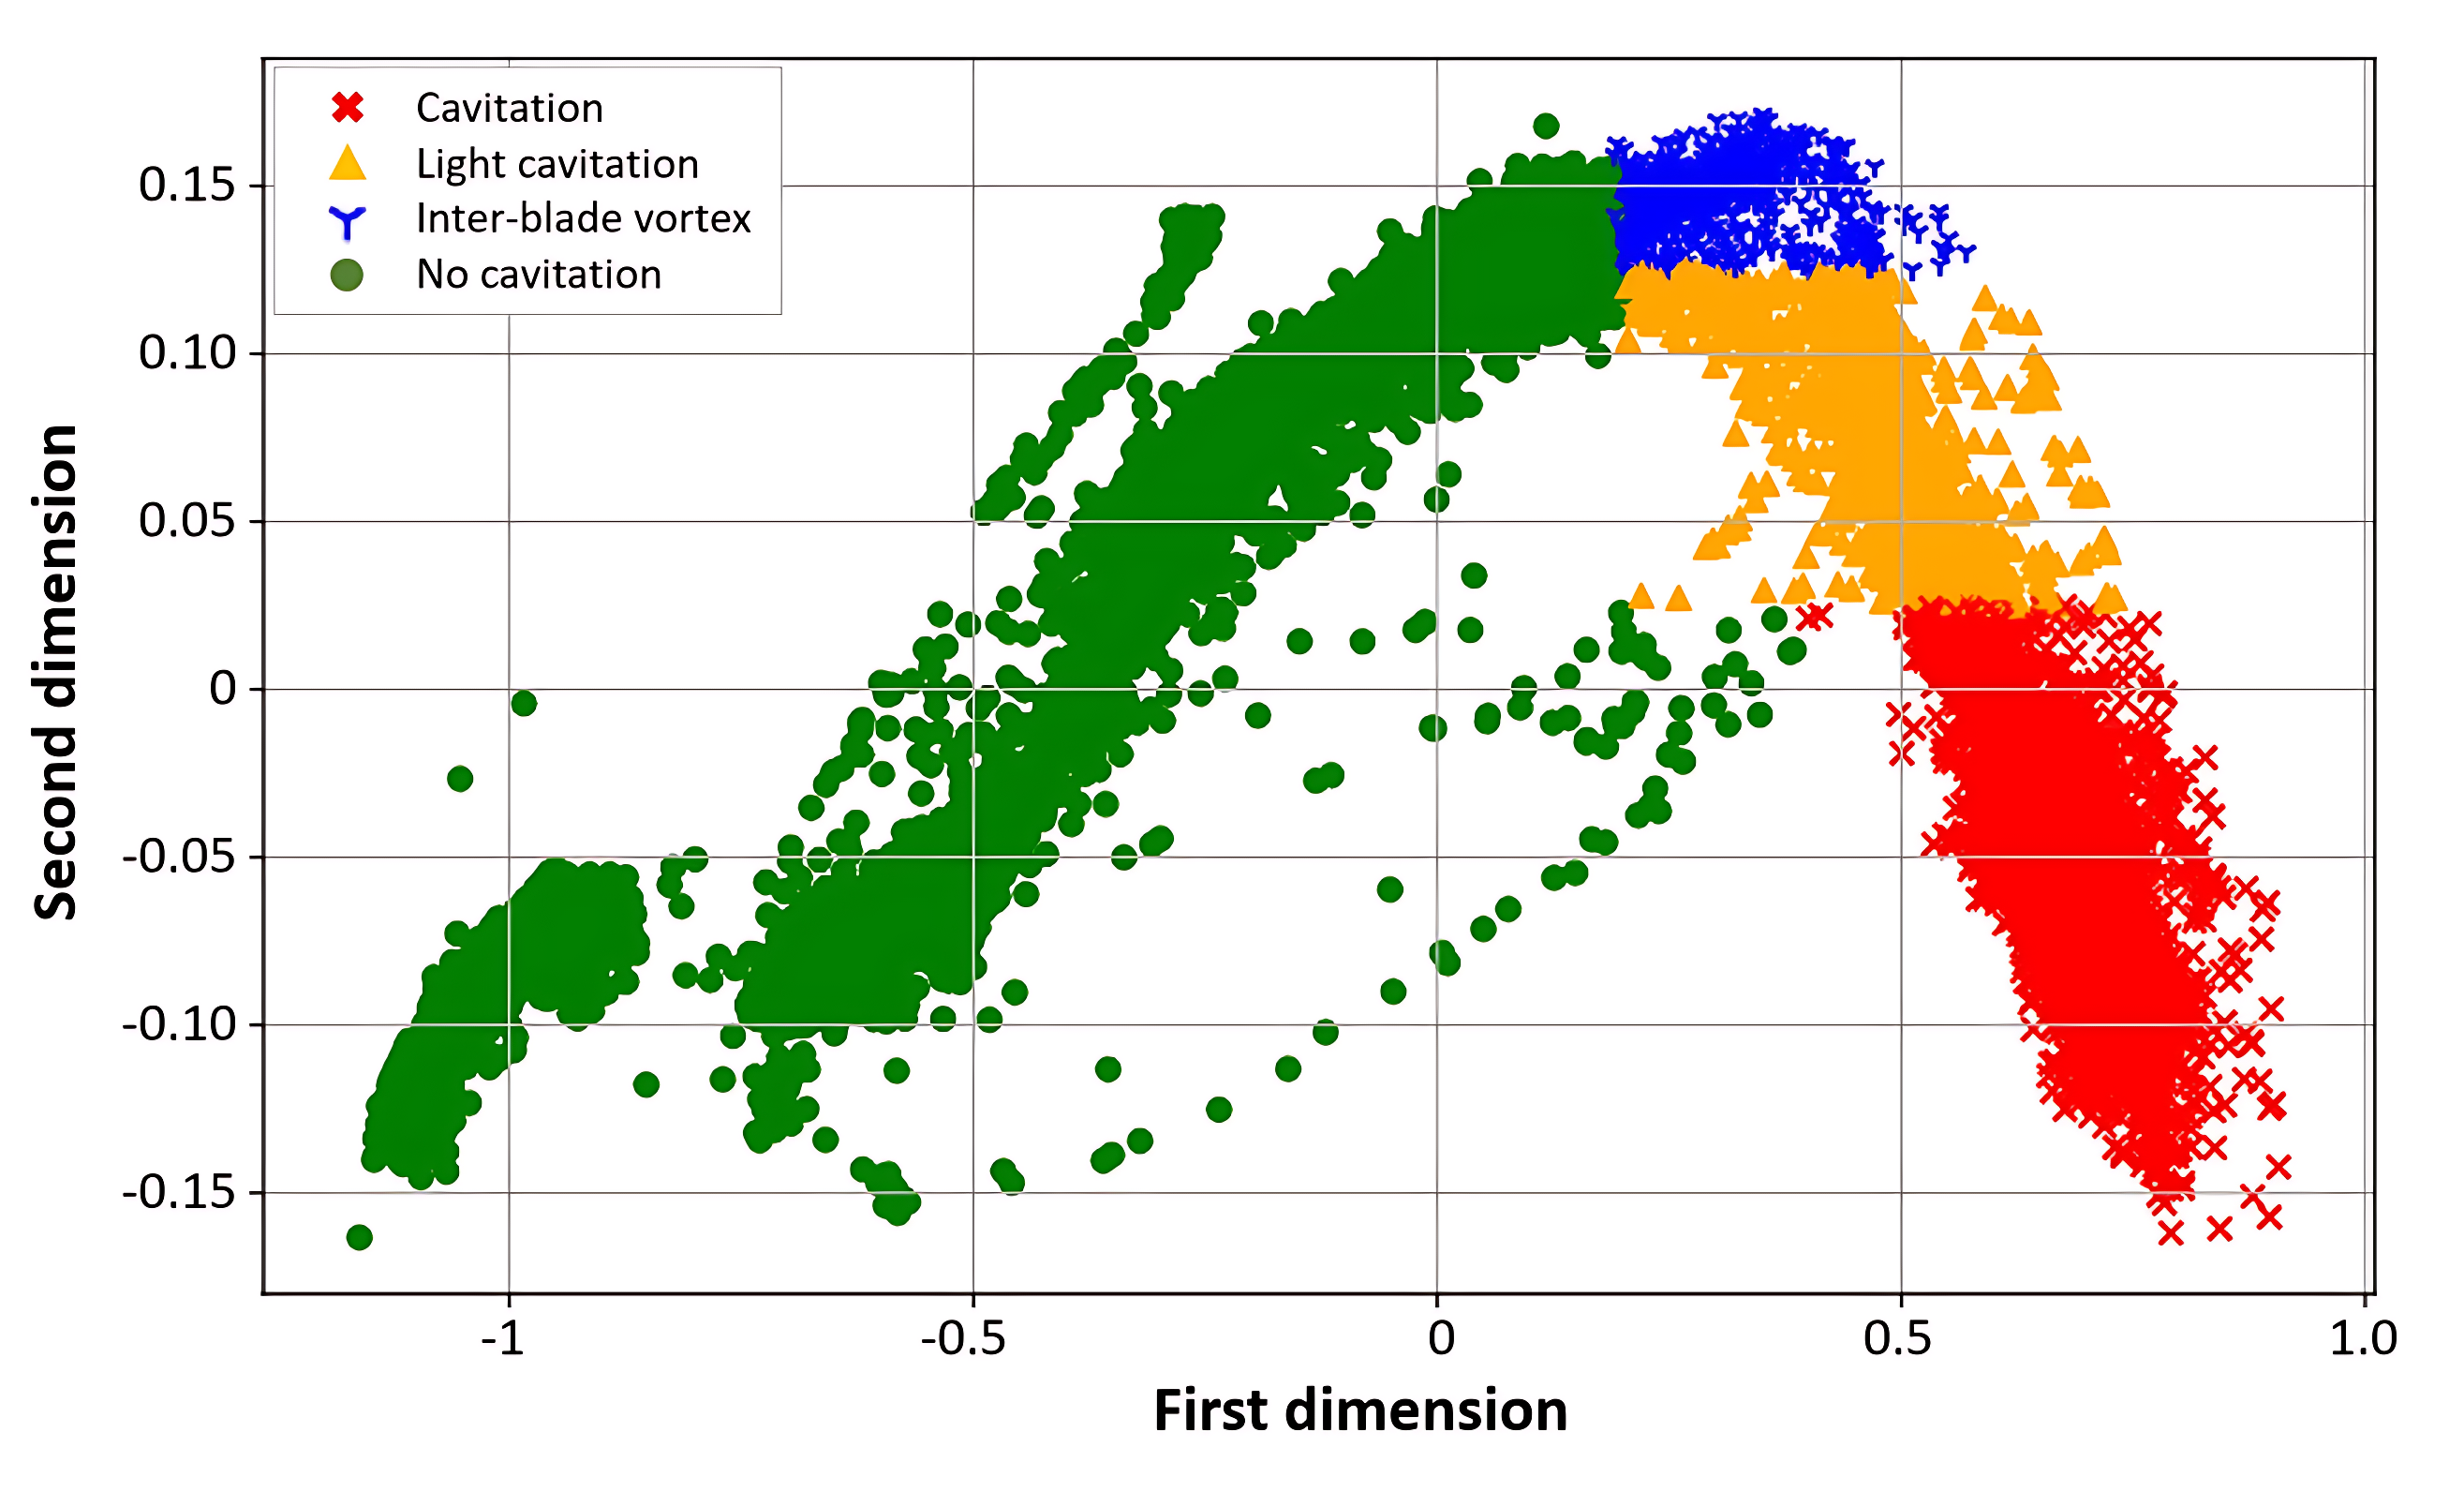
\includegraphics[width=.8\linewidth]{figs/Artigos/amini2022development/Figura6_Upscaler_2K.png}
    \caption{Projeção bidimensional dos dados de operação da turbina obtidos na usina de Ernen, classificando diferentes estados de escoamento: sem cavitação (verde), cavitação leve (amarelo), cavitação plena (vermelho) e vórtices interpalhetas (azul). Fonte: \citeonline{amini2022development}}
    \label{fig:amini2022developmentFig6}
\end{figure}
    
A Figura~\ref{fig:amini2022developmentFig6} exibe o resultado da classificação obtida no ambiente real da usina hidrelétrica. Cada ponto representa um vetor de características projetado em duas dimensões (via redução de dimensionalidade). Observa-se uma separação bem definida entre quatro condições: operação normal, cavitação leve, cavitação severa e presença de vórtices entre pás. Essa distinção confirma a robustez do modelo GMM, mesmo sob ruído operacional e variação de carga.

Em síntese, o estudo demonstra que a combinação entre processamento acústico e aprendizado de máquina é capaz de discriminar, com alta confiabilidade, diferentes estágios de cavitação tanto em condições laboratoriais quanto em ambiente industrial. Os resultados reforçam o potencial dessa abordagem para o monitoramento não intrusivo e o diagnóstico preditivo de turbinas hidráulicas.

Uma análise estatística complementar, realizada a partir do histórico operacional de sete anos da usina, revelou que as turbinas frequentemente operaram em faixas de carga parcial propensas à cavitação. Essa constatação sugere que o fenômeno pode ter contribuído para o desgaste prematuro de componentes e para a redução da eficiência global das máquinas, conforme apresentado na Figura~\ref{fig:amini2022developmentFig7}. Dessa forma, o sistema proposto pelos autores não apenas permite a detecção em tempo real, mas também possibilita o diagnóstico retrospectivo do número de horas em regime cavitante, ampliando seu potencial como ferramenta de manutenção preditiva.

\begin{figure}[H]
    \centering
    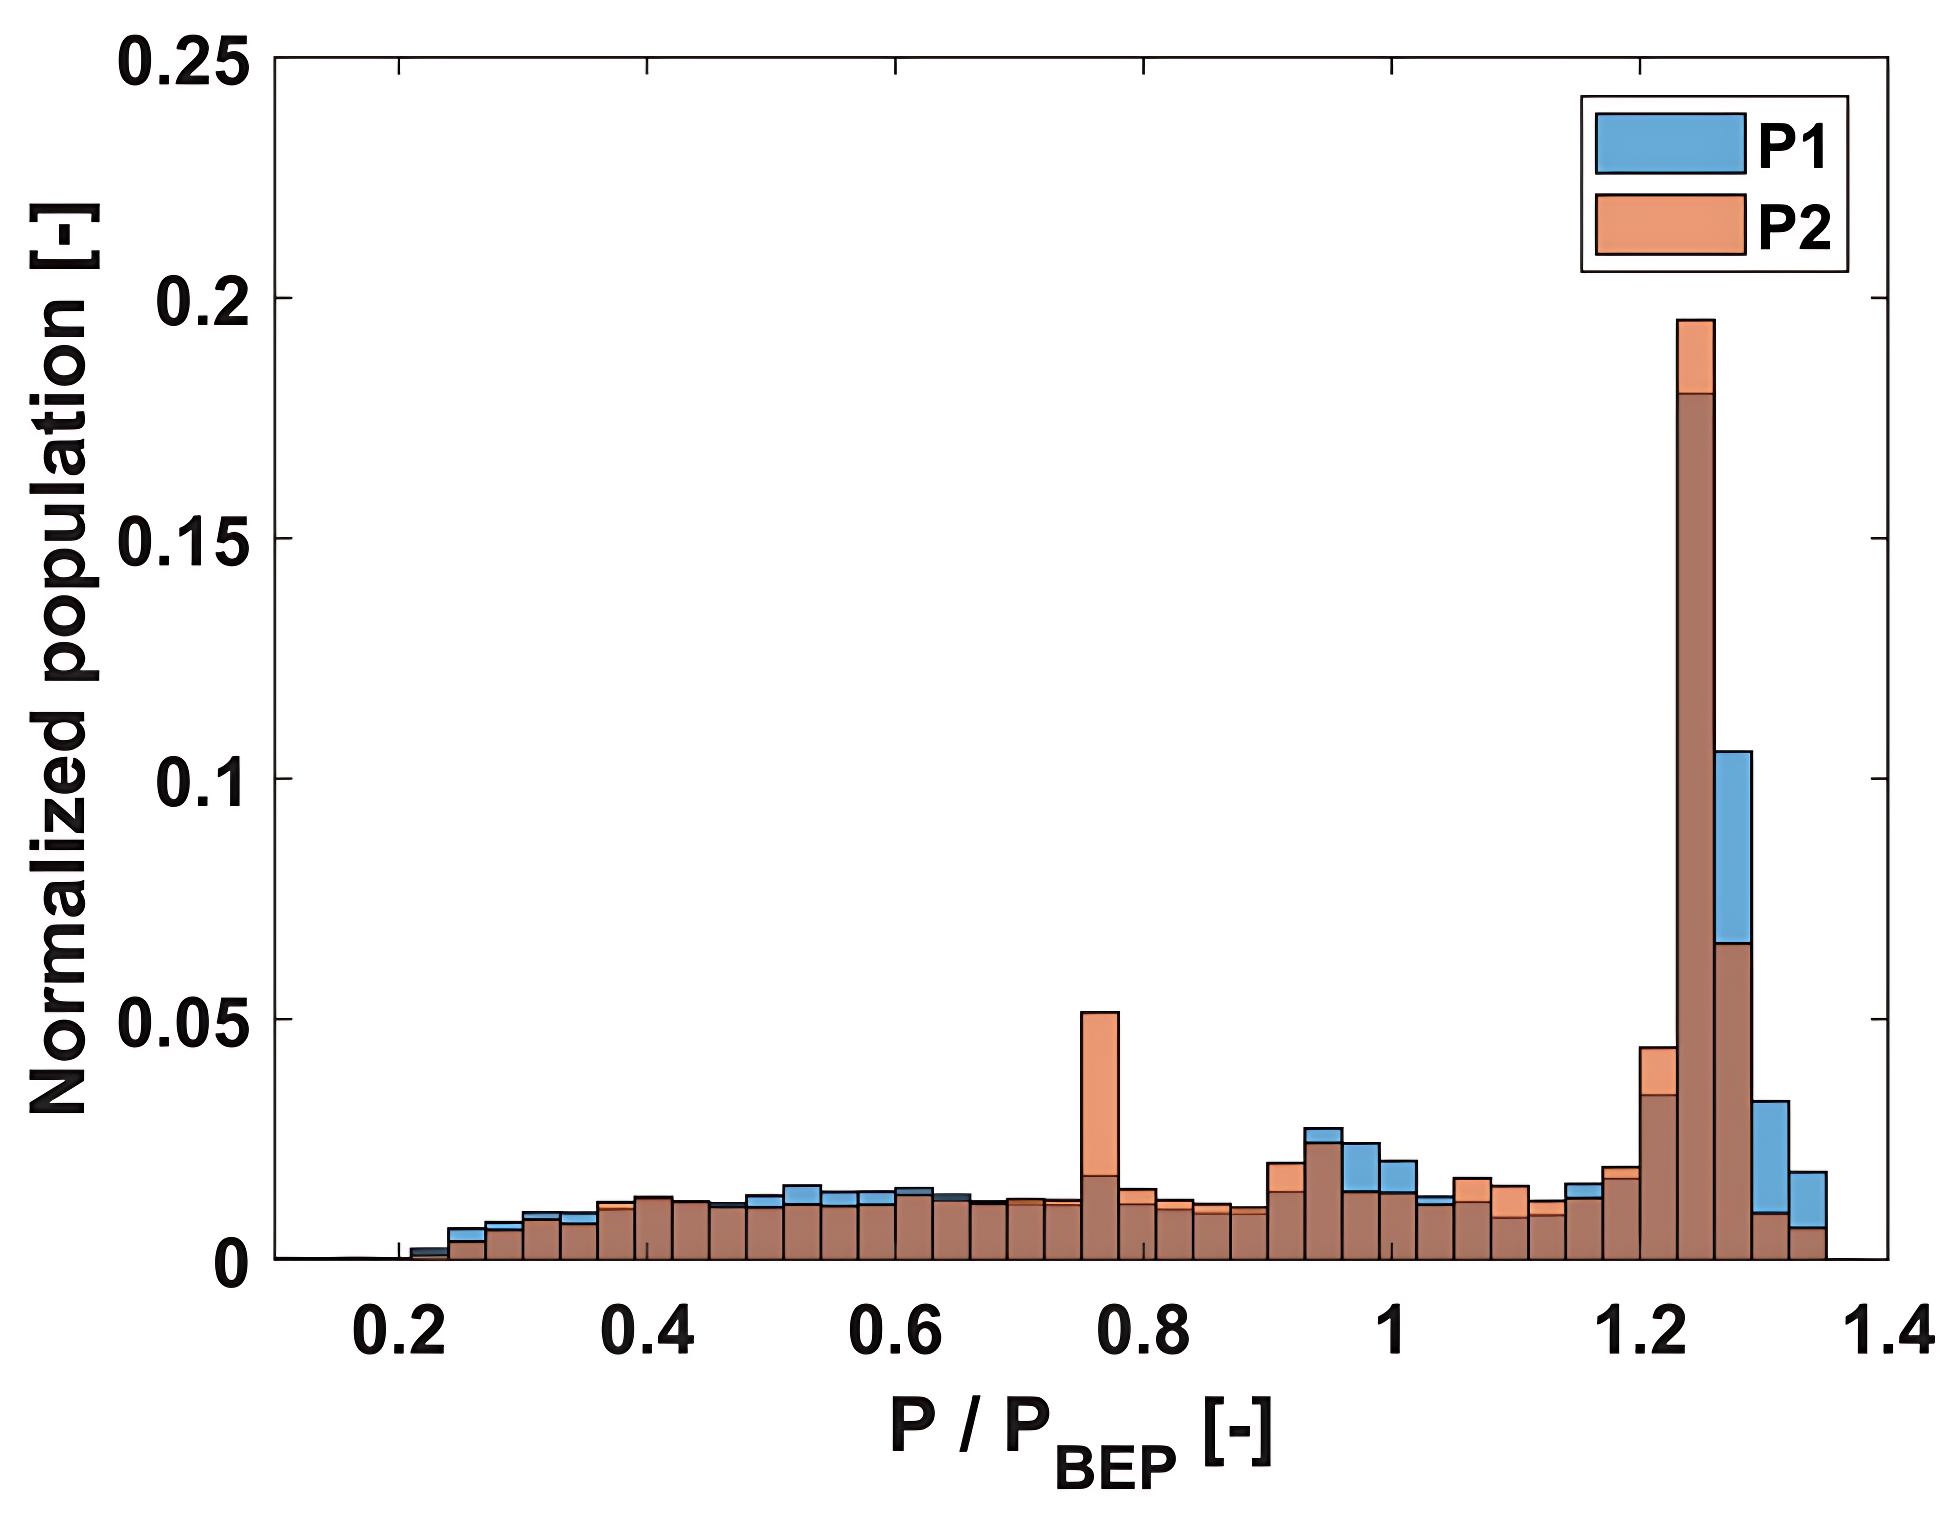
\includegraphics[width=.55\linewidth]{figs/Artigos/amini2022development/Figura7_Upscaler_2K.png}
    \caption{Distribuição normalizada da taxa de potência das duas turbinas idênticas (P1 e P2) da usina hidrelétrica de Ernen ao longo de um período de sete anos. Fonte: \citeonline{amini2022development}}
    \label{fig:amini2022developmentFig7}
\end{figure}

\linespread{1.28}\selectfont
A Figura~\ref{fig:amini2022developmentFig7} evidencia a frequência relativa de operação das duas turbinas, expressa em função da potência normalizada $P / P_{BEP}$, sendo $P_{BEP}$ a potência correspondente ao ponto de melhor eficiência \textit{Best Efficiency Point}. Observa-se que ambas as unidades operaram de forma recorrente acima de $1{,}2\,P_{BEP}$, faixa associada a maior risco de cavitação. Essa distribuição reforça a importância de sistemas de monitoramento contínuo, visto que períodos prolongados nesse regime podem causar erosão nas pás, vibrações excessivas e perdas de desempenho hidráulico. Além disso, a análise mostra a utilidade do sistema proposto não apenas para o acompanhamento em tempo real, mas também como ferramenta de avaliação histórica das condições operacionais e identificação de padrões de desgaste.

\linespread{1.28}\selectfont
Em conclusão, \citeonline{amini2022development} demonstram a viabilidade de um método não intrusivo para detecção de cavitação em turbinas hidráulicas, baseado em sinais acústicos e aprendizado de máquina. O sistema foi validado tanto em condições laboratoriais quanto em escala industrial, apresentando alta precisão na identificação de diferentes regimes de escoamento. Os autores ainda destacam o potencial de aprimoramento futuro por meio da incorporação de algoritmos mais avançados, capazes de distinguir entre diferentes tipos de cavitação e estimar índices de severidade. Tais avanços poderiam ser generalizados para outras configurações de turbinas mediante o uso de técnicas de aprendizado por transferência, ampliando o escopo de aplicação em sistemas hidrelétricos.

\linespread{1.28}\selectfont
A seguir, apresenta-se uma comparação sistemática dos principais tipos de sensores empregados na detecção de cavitação em bombas centrífugas, destacando suas faixas de frequência típicas, vantagens, limitações e aplicações mais adequadas. A Tabela \ref{tab:sensores_cavitacao} sintetiza essas características e proporciona ao leitor uma visão panorâmica dos trade-offs entre custo, sensibilidade e operacionalidade de cada sensor. Com isso, pretende-se facilitar a escolha adequada do sistema de medição conforme o estágio de cavitação, a criticidade do equipamento e o contexto de monitoramento industrial.

\begin{table}[H]
\footnotesize
\centering
\caption{Comparação entre diferentes tipos de sensores utilizados na detecção de cavitação em bombas centrífugas. Adaptado de \citeonline{liu2023review}.}
\label{tab:sensores_cavitacao}
\renewcommand{\arraystretch}{1.3}
\resizebox{\textwidth}{!}{%
\begin{tabular}{p{3.0cm} p{2.4cm} p{4.2cm} p{4.2cm} p{3.2cm}}
\hline
\textbf{Tipo de Sensor} & \textbf{Faixa típica de frequência} & \textbf{Vantagens principais} & \textbf{Limitações} & \textbf{Aplicações mais adequadas} \\ \hline

\textbf{Acelerômetro} &
1Hz – 20kHz &
Baixo custo, ampla disponibilidade e fácil instalação; fornece informações estruturais globais e permite análise conjunta de vibração e ruído. &
Menor sensibilidade para cavitação incipiente; fortemente influenciado por vibrações mecânicas externas e desbalanceamentos. &
Monitoramento geral da condição mecânica e detecção de cavitação moderada ou severa. \\ \hline

\textbf{Sensor de Emissão Acústica} &
100kHz – 1MHz &
Alta sensibilidade a eventos transientes e à cavitação incipiente; capaz de detectar impactos microscópicos e trincas. &
Custo mais elevado e necessidade de acoplamento adequado; suscetível à atenuação do sinal e à interferência estrutural. &
Detecção precoce de cavitação, fadiga e erosão em estágios iniciais. \\ \hline

\textbf{Sensor de Ruído} &
10Hz – 50kHz &
Instalação simples; útil para monitoramento de cavitação intensa e para análises comparativas entre regimes. &
Alta suscetibilidade a ruídos ambientais; dificuldade de calibração e isolamento de fontes. &
Testes experimentais, ensaios comparativos e diagnósticos de cavitação plena. \\ \hline

\textbf{Transdutor de Pressão} &
0 – 5kHz &
Mede diretamente variações de pressão e pulsação hidráulica; fornece informações sobre o escoamento e eficiência volumétrica. &
Baixa resolução temporal para eventos de curta duração; resposta limitada a altas frequências. &
Análise de instabilidades de escoamento, flutuações de pressão e correlação com regimes hidráulicos. \\ \hline
\end{tabular}}
\end{table}

\linespread{1.28}\selectfont
A Tabela \ref{tab:dominio_algoritmos} apresenta uma síntese dos principais “domínios de análise” e “algoritmos de classificação” empregados na detecção de cavitação em bombas centrífugas, conforme relatado por estudos recentes como \citeonline{liu2023review} e \citeonline{Zhang2015}. Esta comparação sistemática permite visualizar como diferentes tipos de sinais (vibração, emissão acústica, ruído, pulsação de pressão ou fusão de sensores) são processados em distintos domínios (tempo, frequência, tempo-frequência ou nível de atributos) e como tais sinais alimentam modelos de aprendizado de máquina ou redes neurais profundas (SVM, Random Forest, CNN, LSTM, entre outros). O conjunto de colunas “Técnicas de Extração de Atributos” e “Algoritmos / Modelos de Classificação” destaca os principais métodos em uso, enquanto a coluna “Referências Representativas” orienta o leitor para os estudos-chave que documentam cada abordagem. Em suma, esta tabela serve como ferramenta de orientação para a seleção de metodologias adequadas ao seu estudo — no qual a ênfase recai sobre o uso de dados de emissão acústica e a implementação simulada de uma CNN-1D — além de evidenciar a evolução do campo em direção a pipelines cada vez mais sofisticados e integrados.
\linespread{1.25}\selectfont
\begin{table}[H]
\footnotesize
\centering
\caption{Domínios de análise e algoritmos utilizados na detecção de cavitação com diferentes tipos de sinais. Fonte: O autor.}
\label{tab:dominio_algoritmos}
\renewcommand{\arraystretch}{1.3}
\resizebox{\textwidth}{!}{%
\begin{tabular}{p{3cm} p{2.9cm} p{4.5cm} p{4.2cm} p{2.8cm}}
\hline
\textbf{Tipo de Sinal} & \textbf{Domínio de Análise} & \textbf{Técnicas de Extração de Atributos} & \textbf{Algoritmos / Modelos de Classificação} & \textbf{Referências Representativas} \\ \hline

\textbf{Vibração} &
Tempo / Frequência &
RMS, curtose, fator de crista, frequência dominante, cepstrum, entropia espectral &
SVM, Random Forest, LSTM, CNN-1D &
\citeonline{liu2023review}, \citeonline{Wang2019} \\ \hline

\textbf{Emissão Acústica} &
Tempo / Frequência &
Amplitude, duração, invólucro retificado (MARSE), contagens, STFT, Wavelet Packet, espectrograma &
CNN-1D, CNN-2D (STFT), SAE, DBN &
\citeonline{liu2023review}, \citeonline{Zhang2015} \\ \hline

\textbf{Ruído} &
Tempo / Frequência &
Análise espectral, densidade de potência, centroides de frequência, coeficientes MFCC &
SVM, k-NN, CNN-2D, Transformer (Spectrogram) &
\citeonline{liu2023review}, \citeonline{Nurvitadhi2017} \\ \hline

\textbf{Pulsos de Pressão} &
Tempo / Frequência &
Média móvel, variância, análise de picos e modulações, componentes harmônicas &
Decision Tree, SVM, LSTM, HMM &
\citeonline{liu2023review} \\ \hline

\textbf{Multissensor} &
Tempo / Frequência / Feature-Level &
Concatenação de atributos normalizados, PCA, autoencoders, STFT sincronizada &
CNN híbrida, redes multimodais, aprendizado por transferência &
\citeonline{liu2023review}, \citeonline{Wang2019} \\ \hline
\end{tabular}}
\end{table}

% \textcolor{red}{Em processo de busca de trabalhos relacionados e leitura para depois escrever esta seção}


% Holford, K.M., et al. (2017). Acoustic emission for monitoring structural integrity: A review. Journal of Acoustic Emission.
% – Revisão clássica e bastante citada sobre princípios e aplicações de EA.

% Pollock, A.A. (2012). Acoustic Emission Inspection. NDT Handbook, ASNT.
% – Livro referência que explica fundamentos e aplicações práticas.

% Grosse, C. U., & Ohtsu, M. (2008). Acoustic Emission Testing. Springer.
% – Base teórica e metodológica, com aplicações em materiais e estruturas.

% Tang, J., et al. (2020). Acoustic emission-based condition monitoring and fault diagnosis of rotating machinery: A review. Applied Acoustics.
% – Excelente revisão ligando EA com análise em máquinas rotativas (seu caso).

% Revisões gerais de EA (Pollock, Holford, Grosse & Ohtsu).

% Aplicações em máquinas rotativas (Tang, Souza).

% Aplicações específicas em cavitação em bombas (Liu).

% \section{Aprendizado de máquinas - CNN}
% \subsection{Introdução}
% \subsection{trabalhos relacionados}
\section{Aprendizado de Máquina}

Esta seção dedica-se à apresentação dos fundamentos conceituais e matemáticos do Aprendizado de Máquina, com ênfase nas abordagens supervisionadas e profundas aplicadas à análise de sinais. Inicialmente, discorrem-se os paradigmas de aprendizado, os principais algoritmos utilizados e suas respectivas áreas de aplicação. Em seguida, introduz-se o Aprendizado Profundo, e as Redes Neurais Multicamada Unidimensionais, destacando seu papel na extração automática de padrões complexos em sinais acústicos, como os gerados por fenômenos de cavitação e falhas incipientes em equipamentos rotativos.

A Inteligência Artificial constitui um campo interdisciplinar dedicado ao desenvolvimento de sistemas computacionais capazes de executar tarefas tradicionalmente associadas à cognição humana, tais como percepção, reconhecimento de padrões, tomada de decisão e raciocínio adaptativo. Seu objetivo central é reproduzir — e, em algumas situações, superar — aspectos do comportamento inteligente por meio de modelos matemáticos, estruturas algorítmicas e processamento de grandes volumes de dados.

Dentro desse panorama, o Aprendizado de Máquina representa uma subárea fundamental, responsável pelo estudo de algoritmos que aprendem a partir de exemplos. Em vez de depender de regras fixas programadas manualmente, esses algoritmos ajustam seus parâmetros internos de forma automática quando expostos a novos dados, aprimorando progressivamente seu desempenho em tarefas específicas. Essa característica torna o AM particularmente adequado a problemas complexos, não lineares ou de natureza estocástica, nos quais abordagens analíticas \mbox{tradicionais apresentam limitações.}

Entre os métodos mais influentes de Aprendizado de Máquina destacam-se as Redes Neurais Artificiais, inicialmente inspiradas em princípios do processamento neural biológico, desde o modelo formal de neurônio proposto por \citeonline{mcculloch1943logical} até as formulações consolidadas em obras clássicas como \citeonline{haykin2001redes}. Embora tais modelos tenham se tornado a base das arquiteturas modernas de aprendizado profundo, eles representam abstrações significativamente simplificadas do funcionamento do sistema nervoso real, empregando ativações contínuas e sincronizadas que não refletem diretamente a natureza pulsada e esparsa da comunicação neuronal biológica.

%Estudos recentes, como o de \citeonline{zheng2022introductory}, ampliam essa discussão ao comparar as Redes Neurais Artificiais convencionais (\textit{Artificial Neural Networks, ANNs}) com as Redes Neurais Pulsadas (\textit{Spiking Neural Networks, SNNs)}, modelos que buscam aproximar de forma mais fidedigna a dinâmica eletrofisiológica observada em neurônios reais. Enquanto as ANNs utilizam funções de ativação contínuas e densas, as SNNs operam com eventos discretos de disparo, \textit{spikes}, permitindo codificação temporal, maior esparsidade e potencial redução significativa no consumo energético. Além disso, diferem quanto aos mecanismos de aprendizagem: ao passo que as ANNs dependem tipicamente do \textit{backpropagation} e de gradientes contínuos, as SNNs investigam regras de aprendizado local inspiradas na biologia, como o \mbox{\textit{Spike-Timing-Dependent Plasticity, STDP.}}
%
%Assim, a literatura contemporânea evidencia uma evolução no entendimento da relação entre modelos computacionais e sistemas biológicos: as ANNs permanecem essenciais para aplicações práticas em larga escala devido à maturidade de suas técnicas de otimização, enquanto as SNNs representam uma fronteira promissora rumo a arquiteturas mais eficientes, esparsas e biologicamente plausíveis, conectando de modo mais direto os princípios da inteligência natural aos mecanismos da inteligência artificial.
%
%Nas redes naturais, cada neurônio, Figura \ref{fig:neuronio} é constituído por dendritos (responsáveis pela recepção dos estímulos provenientes de outras células), pelo corpo celular (que integra e processa os sinais recebidos) e pelo axônio (que transmite a saída para outras células). A comunicação ocorre por meio de impulsos elétricos, cuja frequência determina o nível de ativação do neurônio \citeonline{haykin2001redes}. Ainda que as redes biológicas não transmitam sinais negativos e apresentem organização morfológica extremamente heterogênea, constituem o modelo conceitual que fundamenta a criação das RNAs.
%
%\begin{figure}[H]
%	\centering
%	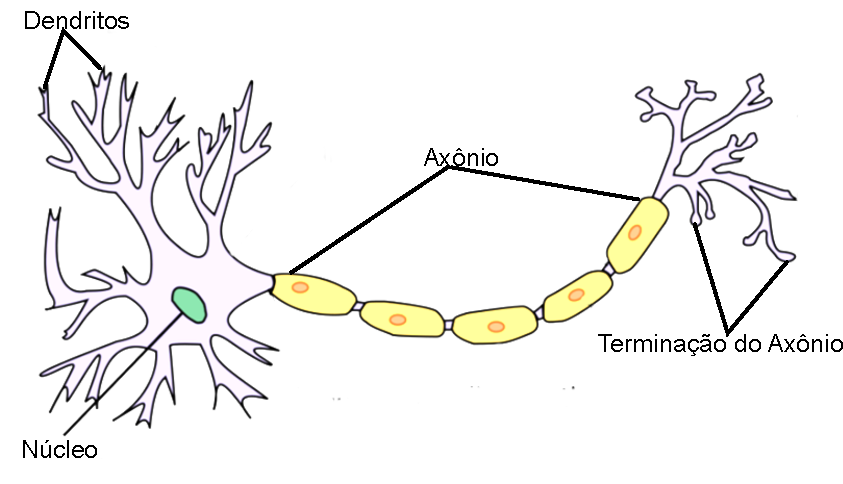
\includegraphics[width=0.65\linewidth]{figs/AprendizadoDeMaquina/Neuronio}
%	\caption{Ilustração de um Neurônio. Adaptado de \citeonline{zheng2022introductory}.}
%	\label{fig:neuronio}
%\end{figure}
%
%O neurônio artificial, por sua vez, é uma abstração computacional que captura os elementos essenciais do processo biológico:
%\begin{enumerate}[label=(\roman*)]
%	\item entradas provenientes do meio ou de outros neurônios;
%	\item sinapses simuladas por pesos, $w_1, w_2, w_3, ... w_n$ que modulam a influência de cada entrada;
%	\item um termo de viés (bias), que desloca a função de ativação e permite maior flexibilidade ao modelo;
%	\item um somador, responsável por combinar as entradas ponderadas;
%	\item uma função de ativação, que limita ou transforma a amplitude do sinal gerado; e
%	\item uma saída, transmitida à próxima camada da rede.
%\end{enumerate}
%
%Em conjunto, múltiplos neurônios artificiais organizados em camadas interconectadas formam arquiteturas capazes de aproximar funções complexas, detectar regularidades em dados ruidosos e extrair características relevantes de sinais multidimensionais. Essa capacidade emergente explica o amplo uso das RNAs em visão computacional, processamento de sinais, reconhecimento de fala, análise temporal e, particularmente neste trabalho, detecção de padrões em sinais de Emissão Acústica.
%
%\begin{figure}[H]
%	\centering
%	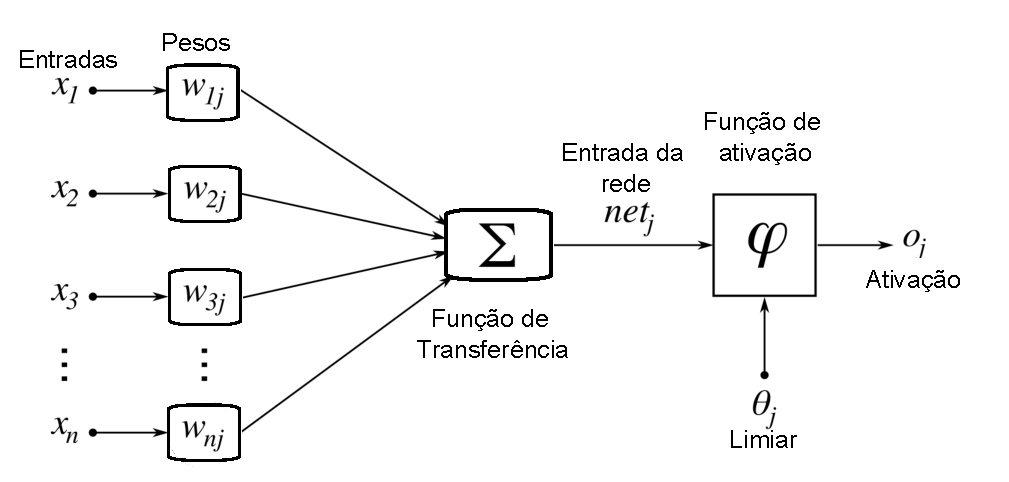
\includegraphics[width=0.85\linewidth]{figs/AprendizadoDeMaquina/NeuronioArtificial}
%	\caption{Neurônio artificial. Fonte: O autor.}
%	\label{fig:artificialneuronmodelenglish}
%\end{figure}
%
%O processo de aprendizado pode ocorrer de diferentes formas, dependendo da disponibilidade e do tipo de informação fornecida ao modelo. De modo geral, o ML é classificado em três categorias principais: aprendizado supervisionado, em que o modelo é treinado com exemplos rotulados; aprendizado não supervisionado, no qual se busca identificar padrões e agrupamentos ocultos em dados não rotulados; e aprendizado por reforço, baseado na interação contínua de um agente com um ambiente para maximizar recompensas acumuladas. Cada uma dessas abordagens apresenta características próprias e é adequada a contextos específicos de aplicação, como classificação, regressão, agrupamento e controle adaptativo.

Um subconjunto mais avançado e especializado do ML é o Aprendizado Profundo, que emprega arquiteturas compostas por múltiplas camadas de processamento, as chamadas redes neurais profundas. Essas estruturas são inspiradas no funcionamento do cérebro humano e são capazes de extrair representações hierárquicas e abstratas dos dados, capturando padrões complexos e não lineares. O DL tem se destacado em aplicações de alto impacto, como reconhecimento de voz e imagem, tradução automática, diagnóstico médico assistido e análise de sinais dinâmicos, devido à sua notável capacidade de generalização e robustez frente a grandes volumes de informação.

Nos últimos anos, a combinação entre aprendizado profundo e dispositivos de alto desempenho, como GPUs e FPGAs, tem ampliado significativamente o escopo de aplicação dessas técnicas, tornando viável a análise em tempo real de dados de alta taxa de amostragem — como os provenientes de sensores acústicos e vibrométricos empregados no monitoramento de máquinas rotativas. Essa integração entre IA e instrumentação digital representa um dos pilares do paradigma da manutenção preditiva inteligente, na qual modelos treinados são utilizados para detectar anomalias, prever falhas e otimizar a operação de sistemas industriais complexos.

%
%O campo do aprendizado de máquina abrange diferentes abordagens de treinamento, cada uma fundamentada na forma como o modelo interage com os dados e aprende a partir deles. De maneira geral, essas abordagens são organizadas em três grandes paradigmas: o aprendizado supervisionado, o aprendizado não supervisionado e o aprendizado por reforço. Cada paradigma apresenta características próprias, vantagens e limitações, sendo aplicável a diferentes tipos de problemas de modelagem, classificação e \mbox{controle em sistemas complexos.}

Os três paradigmas são sistematizados na Figura~\ref{fig:AprendizadoDeMaquinaConceitos}, que apresenta uma visão comparativa das principais estratégias de aprendizado e suas aplicações típicas em contextos industriais. Cada paradigma difere quanto à forma de aprendizado, à disponibilidade de rótulos nos dados e ao tipo de \textit{feedback} recebido durante o processo de treinamento.

\begin{figure}[H]
    \centering
    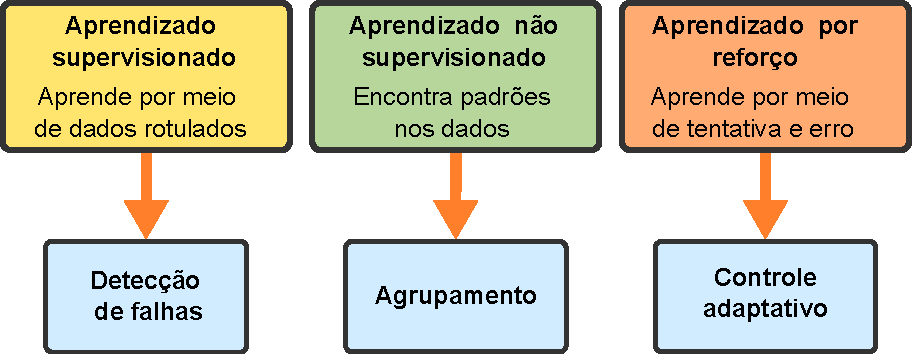
\includegraphics[width=0.7\linewidth]{figs/AprendizadoDeMaquina/AprendizadoDeMaquinaConceitos.pdf}
    \caption{Paradigmas do aprendizado de máquina e exemplos de aplicação industrial.\\Fonte: Em destaque o paradigma utilizado neste trabalha. O autor.}
    \label{fig:AprendizadoDeMaquinaConceitos}
\end{figure}

\begin{itemize}
    \item \textbf{Aprendizado Supervisionado:} Baseia-se na utilização de conjuntos de dados rotulados, nos quais cada amostra possui uma resposta conhecida. O modelo é treinado para aprender a relação entre entradas e saídas, generalizando o comportamento para novos dados. É amplamente empregado em tarefas de classificação e regressão, como a \textbf{detecção de falhas em sensores} ou a previsão de desgaste de componentes em bombas e turbinas.

    \item \textbf{Aprendizado Não Supervisionado:} Opera sobre dados não rotulados, buscando identificar padrões e estruturas ocultas. Utiliza técnicas como o \textit{k-means} ou análise de componentes principais (PCA) para agrupar dados semelhantes ou reduzir dimensionalidade. Essa abordagem é especialmente útil para \textbf{agrupamento de modos de operação}, detecção de anomalias e análise exploratória de sinais industriais.

    \item \textbf{Aprendizado por Reforço:} Difere dos paradigmas anteriores por envolver a interação contínua entre um agente e um ambiente. A cada ação, o agente recebe uma recompensa ou penalidade, aprendendo a maximizar seu desempenho ao longo do tempo. Esse método é aplicado em \textbf{controle adaptativo de processos industriais}, robótica e otimização de sistemas dinâmicos sob condições variáveis.
\end{itemize}

A Figura~\ref{fig:AprendizadoDeMaquinaConceitos} sintetiza graficamente essa classificação, destacando a complementaridade entre os paradigmas de Aprendizado Supervisionado, Não Supervisionado e por Reforço. Essa taxonomia ressalta a relevância das técnicas de \textit{Machine Learning} para a construção de sistemas inteligentes que não apenas identificam falhas, mas extraem conhecimento útil para otimizar processos. Em última análise, o diagrama ilustra o arcabouço conceitual para o desenvolvimento de soluções voltadas à manutenção preditiva, à análise de falhas em componentes mecânicos e ao monitoramento em  com baixa latência de inferência, promovendo a detecção precoce de anomalias e garantindo a maior robustez de decisão no ambiente industrial.

%O aprendizado de máquina engloba uma ampla variedade de algoritmos, cada um com princípios matemáticos e áreas de aplicação específicas. A escolha do modelo mais adequado depende diretamente da natureza dos dados, do objetivo da análise e das restrições computacionais do sistema. De forma geral, entre os principais algoritmos utilizados em ML, são:
%
% \begin{itemize}
%     \item \textbf{Redes Neurais Artificiais (ANNs):} inspiradas no funcionamento biológico do cérebro, compostas por camadas de neurônios interconectados capazes de aprender relações complexas entre variáveis.
%     \item \textbf{Árvores de Decisão e Random Forest:} modelos baseados em regras hierárquicas que realizam divisões sucessivas do espaço de dados, amplamente empregados em classificação e regressão devido à sua interpretabilidade.
%     \item \textbf{Máquinas de Vetores de Suporte (SVMs):} algoritmos que buscam maximizar a margem entre classes, eficazes em conjuntos de dados de alta dimensionalidade e com fronteiras não lineares.
%     \item \textbf{Modelos de Mistura Gaussiana (GMMs):} utilizados para modelar distribuições probabilísticas complexas e realizar agrupamento (clustering) de dados de natureza heterogênea.
%     \item \textbf{Métodos de Ensemble, como Gradient Boosting:} combinam múltiplos modelos fracos (geralmente árvores de decisão) para formar um modelo forte, otimizando o desempenho preditivo e reduzindo o erro de generalização.
%     \item \textbf{Redes Neurais Multicamada (MLP):} arquiteturas profundas projetadas para extrair automaticamente padrões espaciais ou temporais, amplamente empregadas em visão computacional, processamento de áudio e diagnóstico industrial.
% \end{itemize}

%\begin{table}[H]
%\centering
%\caption{Principais algoritmos de aprendizado de máquina e suas características gerais.}
%\label{tab:algoritmos_ml}
%\renewcommand{\arraystretch}{1.3}
%\resizebox{\textwidth}{!}{%
%\begin{tabular}{p{4cm} p{11cm}}
%\hline
%\textbf{Algoritmo} & \textbf{Descrição Geral} \\ \hline
%
%\textbf{Redes Neurais Artificiais (ANNs)} &
%Inspiradas no funcionamento biológico do cérebro, são compostas por camadas de neurônios interconectados capazes de aprender relações complexas entre variáveis, sendo adequadas para modelar fenômenos não lineares. \\ \hline
%
%\textbf{Árvores de Decisão e Random Forest} &
%Modelos baseados em regras hierárquicas que realizam divisões sucessivas do espaço de dados. São amplamente empregados em tarefas de classificação e regressão, destacando-se pela interpretabilidade e robustez a ruído. \\ \hline
%
%\textbf{Máquinas de Vetores de Suporte (SVMs)} &
%Algoritmos que buscam maximizar a margem entre classes, sendo eficazes em conjuntos de dados de alta dimensionalidade e com fronteiras não lineares, especialmente em classificações binárias. \\ \hline
%
%\textbf{Modelos de Mistura Gaussiana (GMMs)} &
%Utilizados para modelar distribuições probabilísticas complexas, permitindo identificar grupos latentes de dados (\textit{clustering}) em aplicações de natureza heterogênea e não supervisionada. \\ \hline
%
%\textbf{Métodos de Ensemble (ex.: Gradient Boosting)} &
%Combinam múltiplos modelos fracos (geralmente árvores de decisão) para formar um modelo mais robusto, otimizando o desempenho preditivo e reduzindo o erro de generalização. \\ \hline
%
%\textbf{Redes Neurais Multicamada (MLP)} &
%Arquiteturas profundas projetadas para extrair automaticamente padrões espaciais ou temporais por meio de filtros convolucionais, amplamente aplicadas em visão computacional, processamento de sinais acústicos e diagnóstico industrial. \\ \hline
%\end{tabular}}
%\end{table}
%
%Entre esses métodos, as \textbf{Redes Neurais Multicamada (MLP)} merecem destaque por sua capacidade de extrair representações hierárquicas de dados brutos, reduzindo a necessidade de pré-processamento manual. Embora originalmente concebidas para o reconhecimento de imagens, as MLP têm-se mostrado extremamente eficazes na análise de sinais acústicos e séries temporais, como os provenientes de sensores de emissão acústica, devido à sua habilidade em capturar correlações locais \mbox{e padrões de alta frequência.}
%
%A arquitetura típica de uma CNN é composta por diferentes tipos de camadas, cada uma com função específica no processo de aprendizado:
%
%\begin{itemize}
%    \item \textbf{Camadas Multicamada:} realizam a operação de convolução, extraindo padrões locais (por exemplo, bordas em imagens ou picos em sinais de emissão acústica).
%    \item \textbf{Camadas de Pooling:} reduzem a dimensionalidade dos mapas de ativação, preservando as informações mais relevantes e diminuindo o custo computacional.
%    \item \textbf{Camadas Totalmente Conectadas (Fully Connected):} integram as características extraídas nas etapas anteriores para a tomada de decisão final, como a classificação do tipo de falha.
%    \item \textbf{Funções de Ativação (ex., ReLU, sigmoid, softmax):} introduzem não linearidade ao modelo, permitindo capturar relações complexas entre as variáveis e melhorar a capacidade de generalização.
%\end{itemize}
%
%Esses elementos, combinados em múltiplos níveis, formam uma estrutura profunda e adaptável, capaz de aprender automaticamente as representações mais relevantes dos dados — característica essencial para aplicações em manutenção preditiva, diagnóstico de falhas e monitoramento inteligente de sistemas industriais.

\section{Redes Neurais MLP)}

\textcolor{red}{Estou Escrevendo}

%A literatura recente tem demonstrado um crescimento expressivo no interesse por métodos de aprendizado profundo, com diversas arquiteturas, como Redes Neurais Profundas (\textit{Deep Neural Network, DNNs}), Redes de Crença Profunda (\textit{Deep Belief Networks, DBNs}), Redes Neurais Recorrentes (\textit{Recurrent Neural Networks, RNN}), Redes Neurais Multicamada (\textit{Convolutional Neural Networks, MLP}) e Transformers, aplicadas a domínios variados, incluindo visão computacional, reconhecimento de fala, processamento de linguagem natural, bioinformática, análise de imagens médicas, ciências climáticas, inspeção de materiais e outras áreas emergentes. Conforme discutido por \citeonline{cacciari2024hands}, embora múltiplas arquiteturas tenham sido propostas para lidar com problemas unidimensionais, as MLP de uma dimensão, continuam sendo amplamente utilizadas e ainda aparecem com maior frequência na literatura indexada entre 2018 e 2023 do que alternativas mais recentes.
%
%O uso de rede MLP permanece menos difundido quando comparado a CNN-2D e CNN-3D, refletindo uma lacuna de pesquisa que inclui tanto menor volume de publicações quanto menor quantidade de revisões sistemáticas dedicadas exclusivamente ao tema. Ainda assim, \citeonline{cacciari2024hands} destacam que as rede MLP constituem uma tecnologia particularmente adequada para aplicações em tempo real, em virtude de sua menor complexidade computacional e capacidade de lidar diretamente com sinais brutos. Exemplos incluem detecção em espectroscopia Raman, linearização de amplificadores em sistemas 5G, monitoramento de interferência eletromagnética em sistemas de potência, classificação de sinais acústicos cardíacos, análise de áudio ambiental, \mbox{modelagem de fala e classificação de música.}
%
%As Redes Neurais Multicamada Unidimensionais representam uma extensão natural das MLP originalmente aplicadas a imagens, adaptadas para o processamento de sinais temporais. Diferentemente das MLP bidimensionais, nas quais os filtros convolucionais percorrem duas dimensões espaciais (altura e largura da imagem), as rede MLP operam exclusivamente sobre a dimensão temporal dos dados, tornando-as especialmente adequadas para o tratamento de séries temporais, \mbox{vibrações e sinais de emissão acústica (EA)}.
%
%\subsection{Fundamentos da Convolução Unidimensional e Análise Comparativa}
%
%As Redes Neurais Multicamada, embora popularizadas pelo sucesso massivo em tarefas de visão computacional, possuem uma formulação matemática generalizável para dados de diferentes dimensionalidades. Conforme discutido por \citeonline{kiranyaz20211d}, enquanto as CNN-2D se tornaram o padrão de fato para processamento de imagens, a adaptação dessa arquitetura para sinais unidimensionais oferece vantagens estruturais decisivas para o processamento de séries temporais, especialmente em cenários com restrições de hardware e latência.
%
%A operação fundamental de uma rede MLP assemelha-se à filtragem digital clássica (FIR), porém com a distinção crucial de que os coeficientes do filtro (pesos do \textit{kernel}) são parâmetros aprendidos através do algoritmo de \textit{Backpropagation}.
%
%Matematicamente, considere um sinal de entrada $x \in \mathbb{R}^{N}$ e um filtro (kernel) $w \in \mathbb{R}^{K}$, onde $K$ representa o tamanho do kernel (campo receptivo local). A convolução linear direta, \textit{valid padding},  para a $k$-ésima camada e o $j$-ésimo neurônio resulta em um mapa de ativação $y$, definido por \ref{eq:conv1d}:
%
%\begin{equation}
%	y_j[i] = f\left( b_j + \sum_{m=1}^{K} w_j[m] \cdot x[i + m - 1] \right)
%	\label{eq:conv1d}
%\end{equation}
%
%\noindent em que:
%
%\begin{itemize}
%	\item $b_j$ é o viés (\textit{bias}) do $j$-ésimo neurônio;
%	\item $f(\cdot)$ é a função de ativação não linear (tipicamente ReLU, Leaky ReLU ou TanH);
%	\item $i$ denota o índice temporal da sequência de saída.
%\end{itemize}
%
%Diferentemente da convolução 2D, que exige varredura em eixos horizontal e vertical, a operação em Eq. \ref{eq:conv1d} ocorre estritamente ao longo do eixo temporal. Segundo \citeonline{kiranyaz20211d}, essa redução de dimensionalidade implica que tanto a \textit{Forward Propagation} quanto a \textit{Backpropagation} podem ser implementadas como operações vetoriais simples, em oposição às operações matriciais complexas exigidas pelas MLP-2D.
%
%
%Para fins de implementação computacional e futura síntese em hardware, o procedimento de inferência de uma única camada MLP pode ser descrito estruturalmente pelo Algoritmo \ref{alg:conv1d_fwd}.
%
%\begin{algorithm}[H]
%	\caption{Processo de Inferência de uma Camada Convolucional 1D (Forward Propagation)}
%	\label{alg:conv1d_fwd}
%	\begin{algorithmic}[1]
%		\Require Vetor de entrada $x$ de tamanho $N$
%		\Require Kernel (filtro) $w$ de tamanho $K$
%		\Require Viés $b$
%		\Require Função de ativação $f(\cdot)$
%		\Require Passo de deslocamento (\textit{stride}) $S$
%		\Ensure Mapa de características de saída $y$
%		
%		\State $L_{out} \gets \lfloor (N - K)/S \rfloor + 1$ \Comment{Calcula dimensão da saída}
%		\State Inicializar vetor $y$ com zeros de tamanho $L_{out}$
%		
%		\For{$i \gets 0$ \textbf{to} $L_{out} - 1$} \Comment{Loop sobre a posição da janela}
%		\State $soma \gets 0$
%		\For{$k \gets 0$ \textbf{to} $K - 1$} \Comment{Loop sobre o kernel (MAC)}
%		\State $soma \gets soma + w[k] \times x[i \cdot S + k]$
%		\EndFor
%		\State $y[i] \gets f(soma + b)$ \Comment{Aplica viés e não-linearidade}
%		\EndFor
%		
%		\State \Return $y$
%	\end{algorithmic}
%\end{algorithm}
%
%A análise do Algoritmo \ref{alg:conv1d_fwd} evidencia a natureza sequencial e determinística da operação. Os laços aninhados (linhas 3 e 5) representam a operação de \textit{Multiply-Accumulate}, MAC, que é o bloco fundamental de processamento em DSPs e FPGAs. Note-se que, em uma implementação de hardware paralela, o laço interno (linhas 5-7) pode ser desenrolado (\textit{unrolled}), permitindo que todas as multiplicações do kernel ocorram em um único ciclo de \textit{clock}, característica explorada para atingir baixa latência.
%
%A topologia de uma rede MLP típica, conforme proposta por \citeonline{kiranyaz20211d}, divide-se em dois blocos funcionais principais:
%
%\begin{enumerate}
%	\item \textbf{Extração de Características (\textit{Feature Extraction}):} Composta por camadas alternadas de convolução 1D e subamostragem (\textit{pooling}). Nesta etapa, a rede aprende a identificar padrões morfológicos no sinal, como picos, oscilações transientes e variações de frequência, gerando tensores de baixa dimensão que resumem o conteúdo informacional da entrada.
%	\item \textbf{Classificação \textit{(MLP Backend}):} Os mapas de características resultantes são achatados (\textit{flattened}) ou processados via \textit{Global Average Pooling} para alimentar camadas densas, \textit{Fully Connected}, que realizam o mapeamento final para as classes de interesse (ex: ``Normal'' vs. ``Cavitação'').
%\end{enumerate}
%
%Uma vantagem arquitetural apontada por \citeonline{kiranyaz20211d} é a capacidade das MLP-1D de atingirem alta performance com arquiteturas ``rasas'' (\textit{shallow architectures}), frequentemente com apenas duas ou três camadas convolucionais ocultas. Isso contrasta com modelos de visão computacional (como ResNet ou VGG), que demandam dezenas de camadas para capturar hierarquias espaciais complexas.
%
%A distinção entre as abordagens não é apenas uma questão de formato de entrada, mas de eficiência computacional e adequação ao domínio do problema. Em aplicações de monitoramento de máquinas, a prática comum de converter sinais 1D em imagens 2D (via Espectrogramas ou Transformada \textit{Wavelet}) para utilizar as CNN-2D pré-treinadas introduz redundância e custo computacional desnecessário.A Tabela \ref{tab:comp_cnn} sumariza as diferenças estruturais destacadas na literatura.
%
%\begin{table}[H]
%	\centering
%	\footnotesize
%	\caption{Comparativo estrutural entre rede MLP e CNN-2D. Adaptado de \citeonline{kiranyaz20211d}.}
%	\label{tab:comp_cnn}
%	\resizebox{\textwidth}{!}{
%	\begin{tabular}{lll}
%		\toprule
%		\textbf{Critério} & \textbf{rede MLP} & \textbf{CNN-2D} \\
%		\midrule 
%		\textbf{Natureza da Entrada} & Vetor ou Série Temporal & Matriz (Imagem, Espectrograma) \\
%		\textbf{Movimento do Kernel} & Unidimensional (apenas tempo) & Bidimensional (altura e largura) \\
%		\textbf{Complexidade Computacional} & $O(N_k \cdot L)$ & $O(N_k \cdot H \cdot W)$ \\ \textbf{Parâmetros Treináveis} & Baixo (kernels vetoriais) & Alto (kernels matriciais)\\
%		\textbf{Requisito de Hardware} & Baixo (viável em CPU/FPGA simples) & Alto (geralmente requer GPU) \\
%		\textbf{Profundidade da Rede} & Tipicamente Rasa (Compacta) & Profunda\\ \textbf{Tratamento de Dados} & Processa sinal bruto (\textit{raw data}) & Exige conversão tempo-frequência \\
%		\bottomrule
%	\end{tabular}}
%\end{table}
%
%A escolha pela rede MLP neste trabalho é fundamentada nas propriedades de ``Compacidade'' e ``Eficiência Adaptativa'' definidas por \citeonline{kiranyaz20211d}.Primeiramente, a convolução 1D preserva a topologia temporal original do sinal de Emissão Acústica, permitindo que a rede explore correlações de fase e eventos transientes que poderiam ser suavizados ou perdidos em uma conversão para espectrograma.Em segundo lugar, a redução drástica no número de Operações de Multiplicação e Acumulação, MACs, torna a rede MLP inerentemente adequada para implementação em FPGA. Enquanto uma CNN-2D exigiria \textit{buffers} de linha complexos e intenso acesso à memória externa para armazenar mapas bidimensionais intermediários, a rede MLP permite um fluxo de dados simplificado e menor latência de inferência, requisitos mandatórios para o sistema de monitoramento em tempo real proposto.


% \section{FPGA}
% \subsection{Introdução}
% \subsection{trabalhos relacionados}
% \subsection{Otimização - Prunning e Quantização}
\section{Field-Programmable Gate Arrays (FPGAs)}

Nesta seção, discutem-se os princípios de funcionamento, a arquitetura e o fluxo de desenvolvimento de sistemas baseados em Field-Programmable Gate Arrays (FPGAs), dispositivos semicondutores programáveis amplamente utilizados em aplicações de processamento digital em tempo real. São abordadas as principais estruturas internas — como blocos lógicos configuráveis, memórias internas e blocos de DSP, e as vantagens oferecidas por esse tipo de hardware em termos de paralelismo, reconfigurabilidade e eficiência energética. Por fim, destaca-se o potencial dos FPGAs como plataforma para a implementação de algoritmos de aprendizado de máquina embarcados, consolidando seu papel em sistemas inteligentes de monitoramento e diagnóstico industrial.

Os FPGAs são dispositivos semicondutores programáveis que permitem a reconfiguração de sua lógica interna mesmo após a fabricação. Essa característica os diferencia dos \textit{Application-Specific Integrated Circuits} (ASICs), projetados para executar uma única função fixa e imutável. Nos FPGAs, o comportamento do hardware é definido por meio de uma descrição de hardware (\textit{Hardware Description Language},HDL), como VHDL ou Verilog, que é sintetizada em uma matriz de blocos lógicos interconectáveis, possibilitando a criação de circuitos digitais personalizados.

A principal vantagem dessa arquitetura reside na \textbf{reconfigurabilidade}, que permite alterar ou atualizar a funcionalidade do sistema sem modificar o hardware físico. Essa flexibilidade torna os FPGAs especialmente atrativos para prototipagem rápida, validação de novas arquiteturas digitais e desenvolvimento de sistemas embarcados adaptáveis. Além disso, os FPGAs combinam desempenho próximo ao de soluções ASIC com o benefício de um tempo de desenvolvimento significativamente menor. Entre as vantagens mais relevantes, destacam-se:

\begin{itemize}
    \item \textbf{Flexibilidade e reconfigurabilidade pós-produção:} possibilitam ajustes no hardware conforme mudanças de requisitos ou algoritmos;
    \item \textbf{Prototipagem rápida:} permitem testar novas arquiteturas digitais sem necessidade de fabricação de chips dedicados;
    \item \textbf{Adaptação dinâmica:} possibilitam o reuso do mesmo hardware em diferentes aplicações por meio de reprogramação parcial;
	\item \textbf{Alto desempenho e paralelismo:} capazes de executar múltiplas operações simultaneamente, com baixa latência, sendo ideais para aplicações como processamento de sinais, visão computacional, telecomunicações e inferência eficiente de redes neurais.
\end{itemize}

Apesar das vantagens, o uso de FPGAs também apresenta desafios significativos. O desenvolvimento demanda conhecimento especializado em eletrônica digital, linguagens HDL e ferramentas de síntese e roteamento, resultando em uma curva de aprendizado acentuada. Além disso, há limitações intrínsecas relacionadas ao número de blocos lógicos disponíveis, à quantidade de memória interna (BRAM) e ao consumo energético, que pode superar o de soluções ASIC quando operando continuamente.

Nos últimos anos, o avanço das aplicações em Inteligência Artificial e Aprendizado Profundo  impulsionou o uso de FPGAs como plataformas de aceleração computacional. Diferentemente das GPUs, que oferecem paralelismo massivo mas com arquitetura fixa, os FPGAs permitem customizar o fluxo de dados e a precisão dos cálculos, adequando-se ao modelo neural e às restrições de desempenho e energia. Esse fator é particularmente relevante em aplicações de inferência em tempo real, onde o equilíbrio entre latência, \textit{throughput} e consumo energético é crítico.

Um dos avanços mais importantes nessa área é a utilização de técnicas de \textbf{quantização de redes neurais}, que reduzem a precisão numérica dos pesos e ativações (por exemplo, de 32 bits para 8 ou 4 bits), mantendo desempenho próximo ao original e reduzindo drasticamente o custo computacional. Essa abordagem viabiliza a implementação de modelos complexos em hardware reconfigurável, preservando acurácia e eficiência.

Dessa forma, os FPGAs consolidam-se como uma plataforma versátil para aplicações em IA embarcada e processamento de sinais industriais, oferecendo uma solução intermediária entre a flexibilidade dos processadores convencionais e a \mbox{eficiência dos ASICs dedicados.}

Compreendidos os princípios gerais de funcionamento e as motivações que tornam os FPGAs atraentes para aplicações de processamento paralelo e aprendizado de máquina embarcado, torna-se relevante examinar sua estrutura interna com maior detalhe. A compreensão dos blocos constituintes e de suas interconexões é essencial para o correto aproveitamento dos recursos de hardware disponíveis e para o desenvolvimento de arquiteturas otimizadas em termos de desempenho, latência e consumo energético.  

Na subseção a seguir, é apresentada a arquitetura interna de um FPGA moderno, destacando-se seus principais componentes, como blocos lógicos configuráveis, memórias internas, blocos DSP e transceptores seriais, e a forma como esses elementos interagem para viabilizar a implementação de circuitos digitais complexos \mbox{em um ambiente reconfigurável.}

\subsection*{Arquitetura Interna de um FPGA}

O desempenho e a flexibilidade dos FPGAs decorrem diretamente de sua arquitetura interna, representada da Figura~\ref{fig:FPGA_internal_architeture}, projetada para combinar \textit{lógica reconfigurável}, \textit{interconexões programáveis} e \textit{blocos especializados} em um mesmo dispositivo. Essa estrutura hierárquica permite que diferentes funções digitais sejam implementadas em paralelo, de acordo com as necessidades do projeto, tornando o FPGA uma plataforma versátil para aplicações de alta complexidade \citeonline{langhammer2014design}.

\begin{figure}[H]
    \centering
    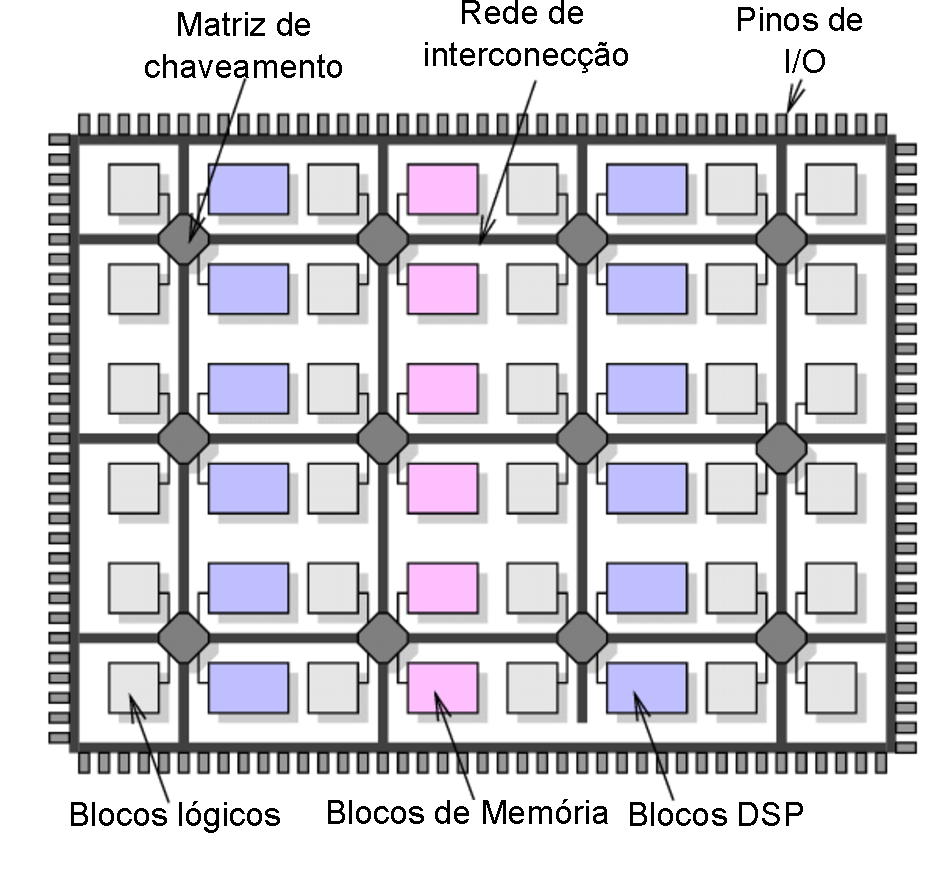
\includegraphics[width=0.65\linewidth]{figs/FPGA/FPGA.pdf}
    \caption{Arquitetura interna de um FPGA. Adaptado de \citeonline{langhammer2014design}}
    \label{fig:FPGA_internal_architeture}
\end{figure}

De modo geral, a arquitetura de um FPGA moderno pode ser compreendida como um arranjo matricial de elementos lógicos, conectados por uma rede de roteamento programável e complementados por blocos dedicados de memória, processamento aritmético e comunicação Figura~\ref{fig:FPGA_internal_architeture}. Essa organização possibilita a construção de circuitos personalizados, capazes de operar de forma determinística e com latência previsível — características essenciais em sistemas embarcados e aplicações de tempo real.

Os principais componentes que compõem essa arquitetura, enfatizando suas funções e a forma como interagem na implementação de sistemas digitais \mbox{complexos são listado a seguir:}

\begin{itemize}
	\item \textbf{Blocos Lógicos Configuráveis (CLBs / Logic Elements)}
	Cada bloco lógico geralmente contém uma \textit{Look-Up Table, LU)}, \textit{flip-flops} (registradores) e lógica de seleção (multiplexadores). As LUTs são usadas para implementar funções lógicas arbitrárias (até uma certa \textit{fan-in}). Os \textit{flip-flops} armazenam estado, e a lógica de interconexão dentro do bloco permite configuração de lógica combinacional ou sequencial.
	
	\item \textbf{Rede de Interconexão Programável}
	Os blocos lógicos são conectados por uma malha (ou rede) de trilhas metálicas (vias, linhas horizontais e verticais) e \textit{switches} programáveis (\textit{crossbars}, multiplexadores, \textit{buffers}). Essa rede determina como os sinais trafegam entre blocos. O desafio de roteamento (satisfazer todas as conexões com restrições de temporização\textit{timing}) é crítico para o desempenho final.
	
	\item \textbf{Blocos de Entrada/Saída (I/O Blocks)}
	Permitem a interface com sinais externos (barramentos, memórias externas, sensores, periféricos). Tipicamente suportam múltiplos padrões de tensão e protocolos (por exemplo, LVDS, PCIe, DDR, \mbox{interfaces de alta velocidade).}
	
	\item \textbf{Blocos de Memória (BRAM / Block RAM)}
	Memórias internas, distribuídas dentro do FPGA, oferecem armazenamento rápido e local para dados intermediários, buffers, tabelas etc. São mais rápidas e eficientes que acessar memória externa.
	
	\item \textbf{Blocos DSP (DSP Slices)}
	Otimizados para operações aritméticas, especialmente multiplicações, multiplicações acumuladas e outras operações de ponto fixo ou ponto flutuante limitada. Permitem acelerar operações pesadas tipicamente usadas em filtros, transformadas, redes neurais etc.
	
	\item \textbf{Transceptores Seriais de Alta Velocidade}
	Alguns FPGAs integram transceptores seriais (links de alta velocidade) que permitem comunicação externa (por exemplo, PCIe, Ethernet de alta velocidade, canais seriais até várias \mbox{dezenas ou centenas de Gbps).}
	
	\item \textbf{Sistemas em Chip (SoC) Integrados}
	Muitos FPGAs modernos incorporam processadores (por exemplo, ARM Cortex, RISC-V) no mesmo chip, compartilhando recursos com a lógica reconfigurável. Isso possibilita uma arquitetura heterogênea: parte do sistema roda em software (no processador), outra parte em lógica personalizada (hardware), com comunicação interna eficiente entre os dois.
	
	\item \textbf{Suporte a Recursos Avançados}
	FPGAs mais recentes podem possuir recursos como reconfiguração parcial dinâmica, blocos de lógica adaptativa (motores de IA, blocos especializados), interconexão multi-DIE (em FPGAs grandes), e suporte a lógica adaptativa para redes neurais (por exemplo, motores de multiplicação de baixa precisão, compressão, suporte a esparsidade, etc.).
\end{itemize}

%A Tabela ~\ref{tab:arquitetura_fpga}, detalha os principais componentes que compõem essa arquitetura, enfatizando suas funções e a forma como interagem na implementação de sistemas digitais complexos:

%\begin{table}[H]
%\centering
%\caption{Principais componentes da arquitetura interna de um FPGA e suas respectivas funções.}
%\label{tab:arquitetura_fpga}
%\renewcommand{\arraystretch}{1.3}
%\resizebox{\textwidth}{!}{%
%\begin{tabular}{p{4cm} p{12cm}}
%\hline
%\textbf{Componente} & \textbf{Descrição e Função Principal} \\ \hline
%
%\textbf{Blocos Lógicos Configuráveis (CLBs / Logic Elements)} &
%Unidades fundamentais de processamento do FPGA, a Figura~\ref{fig:FPGA_CBL} apresente um CBL ilustrativo. Cada CLB contém uma ou mais \textit{Look-Up Tables} (LUTs), registradores (flip-flops) e multiplexadores, permitindo implementar funções lógicas combinacionais ou sequenciais. As LUTs armazenam tabelas de verdade de até $2^n$ entradas, enquanto os flip-flops permitem o armazenamento de estado e sincronização com o clock global. \\ \hline
%
%\textbf{Rede de Interconexão Programável} &
%Responsável por conectar os CLBs, BRAMs, DSPs e demais blocos através de trilhas metálicas horizontais e verticais, controladas por comutadores programáveis (\textit{switch boxes} e \textit{connection boxes}). Essa rede define o fluxo de dados e é determinante para o desempenho do circuito, sendo o processo de roteamento e temporização (timing closure) um dos desafios centrais do projeto em FPGA. \\ \hline
%
%\textbf{Blocos de Entrada/Saída (I/O Blocks)} &
%Interfaceiam o FPGA com dispositivos externos, permitindo comunicação com memórias, barramentos, sensores e periféricos. Suportam múltiplos padrões elétricos (LVCMOS, LVDS, SSTL) e protocolos de alta velocidade, como PCIe, DDR e Ethernet, além de oferecer recursos de calibração e proteção elétrica. \\ \hline
%
%\textbf{Blocos de Memória (BRAM / Block RAM)} &
%Memórias estáticas internas distribuídas na matriz lógica, utilizadas para armazenamento local de dados, buffers de transmissão, tabelas de coeficientes e pesos de redes neurais. Possuem latência extremamente baixa e são configuráveis em diferentes larguras e profundidades. \\ \hline
%
%\textbf{Blocos DSP (DSP Slices)} &
%Unidades aritméticas dedicadas a operações de multiplicação, soma acumulada (MAC) e cálculos de ponto fixo ou ponto flutuante reduzido. São essenciais em tarefas de alto desempenho, como filtragem digital (FIR/IIR), transformadas rápidas (FFT) e aceleração de camadas convolucionais em redes neurais. \\ \hline
%
%\textbf{Transceptores Seriais de Alta Velocidade} &
%Módulos especializados que permitem comunicação externa por meio de canais seriais de alta taxa de transferência (até centenas de Gbps), utilizados em protocolos como PCIe, SATA, Ethernet e JESD204. Possuem circuitos de equalização e controle de clock para integridade de sinal. \\ \hline
%
%\textbf{Sistemas em Chip (SoC) Integrados} &
%FPGAs modernos podem incluir processadores embutidos (ex.: ARM Cortex-A9, RISC-V), formando uma arquitetura heterogênea. Essa integração permite executar parte do sistema em software e parte em hardware, com comunicação interna de alta largura de banda por barramentos AXI (\textit{Advanced eXtensible Interface}). \\ \hline
%
%\textbf{Recursos Avançados e Funcionalidades Adicionais} &
%Modelos recentes incorporam reconfiguração parcial dinâmica (\textit{Partial Reconfiguration}), blocos de lógica adaptativa (AI Engines) e interconexão multi-die (em dispositivos de grande porte). Tais recursos suportam otimizações específicas para aprendizado de máquina, como operações com baixa precisão, compressão de pesos e suporte a sparsidade. \\ \hline
%\end{tabular}}
%\end{table}

\begin{figure}[H]
    \centering
    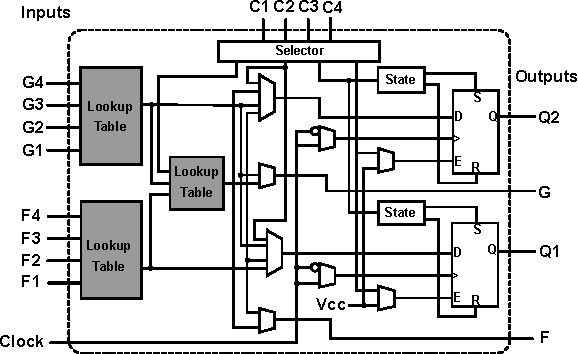
\includegraphics[width=0.8\linewidth]{figs/FPGA/CBL.pdf}
    \caption{Imagem ilustrativa de um \textit{CBL}. Adaptado de \citeonline{genera_technologies_fpga}}
    \label{fig:FPGA_CBL}
\end{figure}

Além disso, o modelo de temporização, timing, nos FPGAs é fundamental: cada sinal tem um caminho entre flip-flops, com restrições de tempo (\textit{setup}, \textit{hold}), e o roteamento de pistas e \textit{buffers} intermediários afetam a latência e taxa máxima de \textit{clock} \mbox{que pode ser alcançada.}

% \subsection*{Fluxo de Desenvolvimento com FPGA}

% Um mapeamento mais detalhado do fluxo de desenvolvimento FPGA típico, com ênfase em aplicações de IA, pode ser descrito da seguinte forma:

% \begin{enumerate}
% \item \textbf{Definição do algoritmo / modelo}
% No caso de IA, inicia-se com o projeto ou escolha da rede neural (topologia, número de camadas, tipo de ativação, quantização, compressão etc.).

% \item \textbf{Quantização / otimização de modelo}
% Para reduzir custo de hardware e latência, frequentemente aplica-se quantização (redução da largura de bits dos pesos e ativações), poda (pruning), compressão esparsa, fatoração ou aproximação de operações.

% \item \textbf{Descrição em HDL ou HLS (High-Level Synthesis)}
% A rede otimizada é então implementada usando linguagens de descrição de hardware (VHDL, Verilog) ou por meio de ferramentas HLS que compilam descrições em C/C++/OpenCL para hardware. As ferramentas HLS permitem abstração mais alta, mas exigem atenção à qualidade do hardware gerado (área, latência, paralelismo).

% \item \textbf{Síntese Lógica}
% A ferramenta converte a descrição de alto nível em uma rede de portas lógicas (LUTs, flip-flops, blocos DSP) lógicas equivalentes.

% \item \textbf{Implementação (Place & Route)}
% O mapeamento lógico é alocado em CLBs, rotas são calculadas pela ferramenta de roteamento, e as interconexões entre blocos são estabelecidas. Aqui ocorrem problemas de congestionamento e restrições de tempo.

% \item \textbf{Análise de Tempo e Ajustes}
% Após roteamento, é feita análise estática de tempo para verificar se os caminhos críticos atendem às restrições de clock. Caso contrário, ajusta-se pipeline, duplicação de lógica, re-rastro, bufferização, restrições de roteamento etc.

% \item \textbf{Geração do Bitstream e Programação}
% O arquivo de configuração (bitstream) é gerado e carregado no FPGA, configurando a interconexão e lógica conforme o design projetado.

% \item \textbf{Verificação / Validação / Testes em Hardware}
% Finalmente, testa-se o circuito configurado (validação funcional, testes de desempenho, consumo, latência, estabilidade).

% \item \textbf{Iterações / Otimizações}
% Muitas vezes, múltiplas iterações são necessárias: ajustes no modelo, re-quantização, pipeline mais fino, divisão em blocos, paralelismo, balanceamento de carga, uso de memória local etc.

% \end{enumerate}

\subsection*{Fluxo de Desenvolvimento com FPGA}

O fluxo de desenvolvimento em FPGAs segue uma sequência bem definida de etapas, que vão desde a concepção do algoritmo até a implementação e validação física do projeto no dispositivo. Esse processo é especialmente relevante em aplicações de Inteligência Artificial (IA) e aprendizado profundo, nas quais o equilíbrio entre desempenho, consumo e utilização de recursos é determinante para a viabilidade do sistema.

O fluxo de desenvolvimento em FPGA, com ênfase em aplicações de Inteligência Artificial, pode ser descrito como uma sequência de etapas encadeadas, que vão desde a definição conceitual do modelo até a validação em hardware e as \mbox{iterações finais de otimização.}

Inicialmente, na \textbf{definição do algoritmo ou modelo}, estabelece-se o comportamento desejado do sistema digital. Em aplicações de IA, essa etapa envolve a escolha ou o projeto de uma arquitetura de rede neural adequada (por exemplo, definição do número de camadas, tipos de ativação, organização MLP e tamanho dos filtros), considerando simultaneamente requisitos de precisão, latência, uso de recursos e complexidade computacional. Trata-se de uma fase predominantemente algorítmica, na qual ainda não se impõem, de forma explícita, as restrições do dispositivo FPGA alvo.

Em seguida, ocorre a \textbf{quantização e otimização do modelo}, cujo objetivo é reduzir o custo computacional e a demanda de recursos de hardware, preservando, tanto quanto possível, a acurácia do modelo. Técnicas como quantização de pesos e ativações (redução da largura de bits), poda (\textit{pruning}), compressão esparsa e fatoração de matrizes são empregadas para diminuir o número de operações e o volume de dados trafegados. Essa etapa é particularmente crítica em FPGAs, dado que LUTs, blocos DSP e BRAMs são recursos finitos e precisam ser utilizados de forma eficiente.

A arquitetura já otimizada é então traduzida para uma \textbf{descrição em HDL ou HLS (High-Level Synthesis)}. Nessa fase, o projeto é implementado em linguagens de descrição de hardware tradicionais, como VHDL ou Verilog, ou em linguagens de mais alto nível (C/C++/OpenCL) que serão sintetizadas por ferramentas de HLS. Embora o HLS facilite o desenvolvimento e aumente o nível de abstração, ele exige uma análise cuidadosa da qualidade do hardware gerado, sobretudo no que diz respeito à área ocupada, ao grau de paralelismo explorado e à latência dos caminhos críticos.

A etapa seguinte corresponde à \textbf{sintese lógica}, na qual a descrição funcional é convertida em uma rede lógica equivalente composta por LUTs, flip-flops, blocos DSP e memórias internas (BRAMs) do FPGA. As ferramentas de síntese aplicam otimizações de lógica booleana, realizam o mapeamento para os recursos específicos do dispositivo e geram uma representação intermediária que servirá de base para o \mbox{processo de implementação física.}

Concluída a síntese, procede-se à \textbf{implementação física (\textit{place \& route})}. Nessa fase, os elementos lógicos são posicionados na matriz do FPGA (\textit{placement}) e as conexões elétricas entre eles são estabelecidas (\textit{routing}). A forma como os blocos (CLBs, DSPs, BRAMs) são distribuídos e interligados impacta diretamente a frequência máxima de operação e o consumo de energia. Congestionamentos na rede de interconexão ou rotas excessivamente longas podem impedir o cumprimento das metas de \mbox{temporização definidas no projeto.}

Após o roteamento, realiza-se a \textbf{análise de tempo e o \textit{timing closure}}. Por meio de análise estática de temporização, verificam-se as restrições de \textit{setup} e \textit{hold} em todos os caminhos relevantes. Caso os caminhos críticos excedam o período de clock especificado, torna-se necessário aplicar técnicas de otimização, tais como inserção de estágios adicionais de pipeline, replicação de lógica, refinamento de restrições ou reorganização de blocos. O objetivo é garantir que o design opere de forma confiável na frequência alvo.

Uma vez satisfeitas as restrições de temporização, procede-se à \textbf{geração do bitstream e programação do dispositivo}. A configuração final é codificada em um arquivo de bits (\textit{bitstream}) que descreve completamente a interconexão e o comportamento interno do FPGA. Esse arquivo é então carregado no dispositivo por meio de interfaces apropriadas (como JTAG, SPI ou USB), configurando-o conforme o projeto desenvolvido.

Na sequência, ocorre a fase de \textbf{verificação e testes em hardware}, em que o design é validado fisicamente no FPGA. São realizados testes funcionais, medições de desempenho, análise de estabilidade e avaliação do consumo energético. Em aplicações de IA, é usual executar a inferência diretamente no hardware, comparando-se a acurácia e o tempo de resposta com aqueles obtidos em simulação ou em plataformas de referência (CPU/GPU), especialmente após a quantização e outras otimizações.

Por fim, o processo raramente se encerra em uma única passagem. Assim, fala-se em \textbf{iterações e otimizações finais}, nas quais o projetista retorna a etapas anteriores para ajustar parâmetros, refinar o pipeline, melhorar o paralelismo, reorganizar \textit{buffers} de memória local e equilibrar a utilização de recursos lógicos e de comunicação. Esse ciclo iterativo é característico do desenvolvimento em FPGA e permite gradualmente aproximar o projeto dos requisitos almejados de latência, \textit{throughput}, \mbox{consumo de energia e área ocupada.}


%O fluxo de desenvolvimento em FPGAs segue uma sequência bem definida de etapas, que vão desde a concepção do algoritmo até a implementação e validação física do projeto no dispositivo. Esse processo, representado de forma resumida na Tabela~\ref{tab:fluxo_fpga}, é especialmente relevante em aplicações de Inteligência Artificial (IA) e aprendizado profundo, nas quais o equilíbrio entre desempenho, consumo e utilização de recursos é determinante para a viabilidade do sistema.

%\begin{table}[H]
%\centering
%\caption{Etapas típicas do fluxo de desenvolvimento em FPGA, com ênfase em aplicações de Inteligência Artificial.}
%\label{tab:fluxo_fpga}
%\renewcommand{\arraystretch}{1.3}
%\resizebox{\textwidth}{!}{%
%\begin{tabular}{p{4cm} p{12cm}}
%\hline
%\textbf{Etapa} & \textbf{Descrição e Objetivos Principais} \\ \hline
%
%\textbf{1. Definição do Algoritmo ou Modelo} &
%Corresponde à etapa inicial do projeto, na qual se define o comportamento desejado do sistema digital. Em aplicações de IA, envolve a escolha ou o desenvolvimento de uma arquitetura de rede neural (número de camadas, tipo de ativação, estrutura MLP, etc.), levando em conta requisitos de precisão, latência e complexidade. \\ \hline
%
%\textbf{2. Quantização e Otimização do Modelo} &
%Visa reduzir a complexidade computacional e o consumo de recursos do FPGA. Técnicas como quantização (redução da largura de bits de pesos e ativações), poda (\textit{pruning}), compressão esparsa e fatoração de matrizes são aplicadas para otimizar o desempenho e minimizar a latência sem comprometer a acurácia do modelo. \\ \hline
%
%\textbf{3. Descrição em HDL ou HLS (High-Level Synthesis)} &
%A arquitetura otimizada é implementada em uma linguagem de descrição de hardware (VHDL, Verilog) ou em linguagens de alto nível (C/C++/OpenCL) compiladas por ferramentas de \textit{High-Level Synthesis}. O HLS facilita o desenvolvimento, mas requer análise criteriosa da qualidade do hardware gerado, especialmente em termos de área, paralelismo e latência. \\ \hline
%
%\textbf{4. Síntese Lógica} &
%Converte a descrição funcional em uma rede lógica equivalente composta por LUTs, flip-flops, blocos DSP e BRAMs. Nessa etapa são aplicadas otimizações automáticas de lógica booleana e mapeamento de recursos específicos do dispositivo alvo. \\ \hline
%
%\textbf{5. Implementação (Place \& Route)} &
%Os elementos lógicos são fisicamente mapeados na matriz do FPGA. O processo de \textit{placement} define a alocação espacial dos blocos (CLBs, DSPs, BRAMs), enquanto o \textit{routing} estabelece as conexões elétricas entre eles. Essa fase é crítica para o desempenho, pois o congestionamento ou roteamento inadequado pode limitar a frequência máxima de operação. \\ \hline
%
%\textbf{6. Análise de Tempo e Ajustes (Timing Closure)} &
%Após o roteamento, é realizada a análise estática de tempo, que verifica o cumprimento das restrições de temporização (\textit{setup} e \textit{hold}). Caso os caminhos críticos ultrapassem o período de clock, aplicam-se técnicas de otimização, como inserção de pipeline, replicação de lógica e ajustes de restrições. \\ \hline
%
%\textbf{7. Geração do Bitstream e Programação} &
%A configuração final é traduzida em um arquivo de bits (\textit{bitstream}), responsável por definir a interconexão e o comportamento interno do FPGA. Esse arquivo é então carregado no dispositivo por meio de interfaces JTAG, SPI ou USB, configurando-o conforme o projeto desenvolvido. \\ \hline
%
%\textbf{8. Verificação e Testes em Hardware} &
%Nesta fase, o design é validado fisicamente. São realizados testes de funcionalidade, desempenho, estabilidade e consumo energético. Em projetos de IA, é comum realizar inferência direta no FPGA para medir a precisão do modelo após quantização e integração. \\ \hline
%
%\textbf{9. Iterações e Otimizações Finais} &
%O ciclo de desenvolvimento raramente é linear. Geralmente, diversas iterações são necessárias para ajustar parâmetros, refinar o pipeline, melhorar o paralelismo, reorganizar buffers de memória local e equilibrar a utilização de recursos lógicos e de comunicação. \\ \hline
%\end{tabular}}
%\end{table}

O processo de desenvolvimento e otimização de projetos em FPGA pode ser sintetizado na Figura~\ref{fig:FluxoDesenvolvimentoFPGA}, que apresenta, de forma esquemática, o ciclo completo desde a definição inicial do algoritmo até a validação em hardware. Esse fluxo evidencia o caráter iterativo do desenvolvimento em dispositivos reconfiguráveis, no qual a cada etapa — da modelagem à implementação física — o projetista deve buscar o equilíbrio entre desempenho, \mbox{consumo e utilização de recursos lógicos.}

\begin{figure}[H]
    \centering
    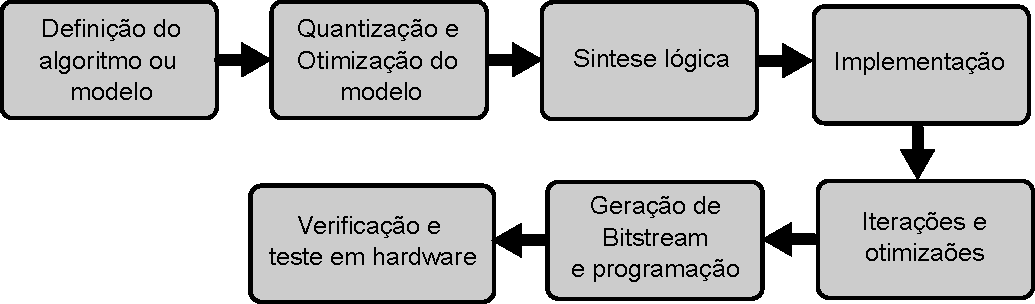
\includegraphics[width=0.8\linewidth]{figs/FPGA/FluxoOtimização.pdf}
    \caption{Fluxo de desenvolvimento e otimização de projetos em FPGA. O autor.}
    \label{fig:FluxoDesenvolvimentoFPGA}
\end{figure}

A Figura~\ref{fig:FluxoDesenvolvimentoFPGA} destaca a sequência típica de etapas: inicia-se pela definição do modelo ou algoritmo, seguida pela quantização e otimização, que reduzem a complexidade computacional. Na sequência, a descrição em HDL ou por meio de ferramentas de HLS permite traduzir o comportamento algorítmico em lógica digital reconfigurável. As fases de síntese e \textit{place \& route} realizam o mapeamento físico do projeto sobre os blocos lógicos e interconexões do FPGA, seguidas da análise de temporização, responsável por assegurar que todas as restrições de tempo de propagação sejam satisfeitas. Por fim, ocorre a geração do \textit{bitstream}, etapa na qual o projeto é convertido em um arquivo de configuração e carregado no dispositivo para verificação e validação funcional.

Ao final do ciclo, ajustes e otimizações adicionais são frequentemente necessários, refletindo o caráter experimental e aprimorável do processo. Essa natureza iterativa é fundamental em aplicações de Inteligência Artificial, nas quais a eficiência do hardware depende diretamente do grau de paralelismo, da largura de barramento e da arquitetura da rede neural mapeada no FPGA.


O sucesso do projeto depende da integração eficiente entre as etapas de síntese, implementação e análise de tempo. Pequenas variações no roteamento ou na granularidade do paralelismo podem impactar significativamente a taxa máxima de \textit{clock} e o consumo energético do sistema, sobretudo em aplicações de aprendizado profundo com restrições de latência e \textit{throughput}.

No contexto de aplicações de Inteligência Artificial, algumas etapas do fluxo de desenvolvimento em FPGA exigem atenção especial para garantir eficiência e desempenho. O \textit{quantization-aware training}, por exemplo, permite que o modelo seja treinado levando em consideração os efeitos da quantização, preservando a acurácia mesmo com representações de baixa precisão. O mapeamento eficiente de multiplicações binárias ou quantizadas — frequentemente implementadas em blocos DSP — é essencial para maximizar o paralelismo e reduzir o consumo de área lógica. Da mesma forma, o suporte à ``esparsidade'' de valores nulos e a utilização otimizada de memórias locais (BRAM e URAM) são fatores decisivos para minimizar a dependência de acessos à memória externa, os quais representam um dos principais gargalos de desempenho em arquiteturas reconfiguráveis.  

Essas estratégias de otimização, quando bem empregadas, tornam os FPGAs especialmente adequados para aplicações embarcadas de IA e aprendizado profundo, nas quais o equilíbrio entre consumo energético, latência e throughput é determinante para a viabilidade prática do sistema.

% A subseção a seguir apresenta uma análise comparativa das principais vantagens e limitações desses dispositivos, considerando seu uso em aceleração de algoritmos de inteligência artificial.

%\subsection*{Vantagens e Desvantagens dos FPGAs (na perspectiva de IA)}
%
%O uso de FPGAs em aplicações de Inteligência Artificial apresenta um conjunto de vantagens que os torna particularmente atrativos para a implementação de algoritmos de aprendizado profundo e de processamento de sinais em tempo real. Em especial, destacam-se aspectos como flexibilidade de reconfiguração, exploração de paralelismo em nível de hardware e potencial de eficiência energética em cenários de inferência embarcada e de borda, \textit{edge computing}. A seguir, são sintetizados alguns dos principais pontos fortes associados a essa tecnologia:
%
%\begin{itemize}
%	\item \textbf{Reconfigurabilidade e adaptabilidade:} possibilita modificar o hardware após a fabricação, permitindo ajustar a arquitetura à medida que o modelo de IA ou os requisitos do sistema evoluem, sem necessidade de projetar um novo circuito integrado dedicado.
%	
%	\item \textbf{Paralelismo massivo:} os recursos lógicos internos permitem a execução simultânea de múltiplas operações, explorando de forma direta o paralelismo intrínseco de redes neurais, filtros convolucionais e demais blocos de processamento distribuído.
%	
%	\item \textbf{Baixa latência e previsibilidade temporal:} a ausência de camadas intermediárias de software e de sistemas operacionais complexos favorece um comportamento determinístico, com latência reduzida e previsível — característica essencial em aplicações em tempo real e em sistemas de controle crítico.
%	
%	\item \textbf{Eficiência energética:} quando adequadamente otimizados, projetos em FPGA podem alcançar maior eficiência em termos de operações por joule (ops/J) do que soluções baseadas exclusivamente em GPU, especialmente em cenários de inferência local e dispositivos de borda.
%	
%	\item \textbf{Customização de precisão:} o suporte à implementação de operações com diferentes larguras de palavra (por exemplo, formatos binários, ternários ou de 4–8 bits) permite ajustar o uso de recursos de hardware de acordo com a tolerância do modelo à quantização, equilibrando acurácia e custo computacional.
%	
%	\item \textbf{Integração de funções heterogêneas:} em um único chip, é possível combinar blocos de controle, interfaces de comunicação, módulos de pré-processamento e pós-processamento de sinais, reduzindo a latência de comunicação entre etapas e o consumo global do sistema.
%\end{itemize}


%O uso de FPGAs em aplicações de Inteligência Artificial apresenta um conjunto de vantagens que os tornam altamente atrativos para a implementação de algoritmos de aprendizado profundo e processamento de sinais em tempo real. A Tabela~\ref{tab:fpga_vantagens} sintetiza os principais aspectos positivos observados na literatura e na prática industrial, destacando sua flexibilidade, paralelismo e eficiência energética — fatores determinantes para aplicações embarcadas e de borda (\textit{edge computing}).
%
%\begin{table}[H]
%\centering
%\caption{Principais vantagens dos FPGAs em aplicações de Inteligência Artificial.}
%\label{tab:fpga_vantagens}
%\renewcommand{\arraystretch}{1.3}
%\resizebox{\textwidth}{!}{%
%\begin{tabular}{p{4cm} p{12cm}}
%\hline
%\textbf{Vantagem} & \textbf{Descrição} \\ \hline
%
%\textbf{Reconfigurabilidade e adaptabilidade} &
%Permite modificar o hardware após a fabricação, possibilitando ajustes à medida que o modelo ou os requisitos do sistema evoluem, sem a necessidade de novos projetos físicos. \\ \hline
%
%\textbf{Paralelismo massivo} &
%Os recursos lógicos permitem a execução simultânea de múltiplas operações, explorando o paralelismo intrínseco de redes neurais e filtros convolucionais. \\ \hline
%
%\textbf{Baixa latência e previsibilidade temporal} &
%A ausência de camadas intermediárias de software garante processamento determinístico, ideal para aplicações em tempo real e controle crítico. \\ \hline
%
%\textbf{Eficiência energética} &
%Projetos bem otimizados em FPGA podem atingir maior eficiência em operações por joule (ops/J) do que GPUs, especialmente em aplicações de inferência local e dispositivos de borda. \\ \hline
%
%\textbf{Customização de precisão} &
%Suporte à implementação de operações com diferentes larguras de palavra (binária, ternária, 4–8 bits), ajustando o consumo de recursos conforme a tolerância do modelo à quantização. \\ \hline
%
%\textbf{Integração de funções heterogêneas} &
%Permite integrar, em um único chip, blocos de controle, interfaces de comunicação, pré-processamento e pós-processamento de sinais, reduzindo latência e consumo. \\ \hline
%\end{tabular}}
%\end{table}

%Apesar de seus benefícios, o uso de FPGAs em aplicações de Inteligência Artificial também apresenta limitações e desafios que precisam ser cuidadosamente considerados no processo de projeto. Em particular, destacam-se restrições de recursos físicos, maior complexidade de desenvolvimento e um ciclo de projeto mais longo quando comparado a plataformas mais convencionais. A seguir, são sintetizados alguns dos principais pontos críticos associados a essa tecnologia:
%
%\begin{itemize}
%	\item \textbf{Recursos limitados:} a quantidade de blocos lógicos, unidades DSP e memórias internas (BRAMs) disponível em um FPGA é finita. Redes neurais de grande porte ou modelos com elevado número de parâmetros podem exceder a capacidade do dispositivo, exigindo estratégias adicionais de quantização, poda ou \mbox{particionamento do modelo.}
%	
%	\item \textbf{Complexidade de projeto:} o desenvolvimento em FPGA demanda domínio de linguagens de descrição de hardware (como VHDL e Verilog) ou de fluxos baseados em \textit{High-Level Synthesis}, além de conhecimento em síntese lógica, fechamento de temporização e otimização de desempenho. Esse conjunto de competências torna a curva de aprendizado mais íngreme quando comparado a frameworks de alto nível em CPU ou GPU.
%	
%	\item \textbf{Desempenho inferior a ASICs dedicados:} embora ofereçam flexibilidade e reconfigurabilidade, FPGAs não alcançam, em geral, a mesma densidade lógica nem a mesma eficiência energética de circuitos integrados de aplicação específica (ASICs) projetados sob medida para uma determinada rede ou tarefa.
%	
%	\item \textbf{Consumo em uso contínuo:} em aplicações de longa duração e alta taxa de utilização, o consumo energético total pode superar o de soluções especializadas ou de chips dedicados, sobretudo quando o projeto não explora plenamente recursos de desligamento parcial, \textit{clock gating} ou outras técnicas de economia de energia.
%	
%	\item \textbf{Tempo de desenvolvimento elevado:} etapas como implementação física, \textit{place \& route}, fechamento de temporização, \textit{timing closure}, balanceamento de pipeline e ajuste fino de restrições podem demandar múltiplas iterações, aumentando significativamente o tempo total de desenvolvimento em comparação com arquiteturas puramente de software.
%	
%	\item \textbf{Gargalos de memória externa:} o acesso frequente à memória DRAM externa pode introduzir latência adicional e elevar o consumo de energia. Isso exige estratégias cuidadosas de uso de memória local (BRAMs, buffers e caches) e de reutilização de dados para evitar que a banda de memória se torne o \mbox{principal limitante do desempenho.}
%	
%	\item \textbf{Desafios de quantização e precisão:} a necessidade de reduzir a largura de palavra (por exemplo, para 8, 4 ou até 1–2 bits) a fim de caber no FPGA pode conduzir à degradação da acurácia do modelo. Encontrar o equilíbrio entre custo de hardware e desempenho preditivo é uma tarefa não trivial, frequentemente exigindo técnicas de \textit{quantization-aware training} e experimentação extensiva.
%\end{itemize}


%Apesar de seus benefícios, o uso de FPGAs também apresenta limitações que devem ser consideradas durante o processo de desenvolvimento. Conforme resumido na Tabela~\ref{tab:fpga_desvantagens}, os principais desafios envolvem restrições de recursos físicos, complexidade de projeto, e tempo de desenvolvimento — fatores que demandam conhecimento especializado em arquitetura digital e ferramentas de síntese.
%
%\begin{table}[H]
%\centering
%\caption{Principais desvantagens e desafios no uso de FPGAs para aplicações de IA.}
%\label{tab:fpga_desvantagens}
%\renewcommand{\arraystretch}{1.3}
%\resizebox{\textwidth}{!}{%
%\begin{tabular}{p{4cm} p{12cm}}
%\hline
%\textbf{Desvantagem} & \textbf{Descrição} \\ \hline
%
%\textbf{Recursos limitados} &
%A quantidade de blocos lógicos, DSPs e memórias internas é finita; redes neurais de grande porte podem exceder a capacidade disponível. \\ \hline
%
%\textbf{Complexidade de projeto} &
%O desenvolvimento requer domínio de linguagens de descrição de hardware (VHDL, Verilog) e ferramentas de síntese, além de experiência com restrições temporais e otimização de performance. \\ \hline
%
%\textbf{Desempenho inferior a ASICs} &
%Embora flexível, o FPGA não atinge a mesma densidade lógica nem a eficiência energética de um ASIC dedicado para a mesma aplicação. \\ \hline
%
%\textbf{Consumo em uso contínuo} &
%Para tarefas de longa duração, o consumo energético pode superar soluções otimizadas ou chips dedicados. \\ \hline
%
%\textbf{Tempo de desenvolvimento elevado} &
%Etapas como roteamento, fechamento de temporização (\textit{timing closure}) e balanceamento de pipeline aumentam significativamente o tempo de iteração. \\ \hline
%
%\textbf{Gargalos de memória externa} &
%O acesso à memória DRAM externa pode introduzir latência e elevar o consumo de energia, exigindo estratégias de uso eficiente da memória local. \\ \hline
%
%\textbf{Desafios de quantização e precisão} &
%A redução excessiva da precisão pode degradar a acurácia do modelo; equilibrar custo de hardware e desempenho é uma tarefa complexa. \\ \hline
%\end{tabular}}
%\end{table}

%Diante desse conjunto de vantagens e limitações, o uso de FPGAs em aplicações de Inteligência Artificial caracteriza-se por um claro compromisso entre desempenho, flexibilidade e complexidade de desenvolvimento. 
%
%Por um lado, a possibilidade de explorar paralelismo em nível de hardware, customizar a precisão numérica e integrar, em um único dispositivo, funções de aquisição, processamento e decisão torna os FPGAs particularmente atraentes para sistemas de monitoramento em tempo real baseados em aprendizado de máquina. Por outro, a necessidade de lidar com recursos restritos, fluxos de projeto mais complexos e desafios de quantização demanda uma fase prévia de estudo e modelagem cuidadosa antes de se partir para a implementação física. 
%
%Nesse contexto, o presente trabalho concentra-se em um \textit{estudo de viabilidade} por meio de simulação de uma arquitetura baseada em rede MLP embarcada em FPGA, utilizando o framework FINN como ferramenta de apoio ao mapeamento em hardware.
%



%O objetivo é compreender, de forma sistemática, como os trade-offs entre acurácia, latência e uso de recursos podem ser equilibrados em um cenário de detecção de cavitação por emissão acústica, fornecendo subsídios técnicos para futuras etapas de prototipagem e implementação real.


\subsection{Otimização de IA em FPGAs: técnicas, desafios e tendências}

Para que redes neurais sejam mapeadas de forma eficiente em FPGAs, é necessário aplicar um conjunto de técnicas de otimização que atuam simultaneamente sobre a arquitetura do modelo, a representação numérica dos dados e a própria organização interna do hardware, garantindo assim um melhor aproveitamento dos recursos disponíveis.

Em linhas gerais, essas estratégias buscam reduzir latência, consumo de energia e uso de área lógica, preservando, tanto quanto possível, a acurácia do modelo. A seguir, são apresentadas algumas das principais abordagens relatadas na literatura recente para aceleração de redes neurais em FPGAs:

\begin{itemize}
	\item \textbf{Quantização:} consiste em reduzir a largura de bits de pesos e ativações (por exemplo, para 8, 4, 2 ou mesmo 1 bit), diminuindo o uso de DSPs e de memória interna. Quando combinada com treinamento ciente de quantização (\textit{quantization-aware training}), essa técnica permite obter modelos mais compactos com perda limitada de desempenho, sendo uma das bases de muitos fluxos de implementação em FPGA.
	
	\item \textbf{Poda e exploração de esparsidade:} remove conexões cujos pesos são próximos de zero, reduzindo o número de operações aritméticas e acessos à memória. Para que o ganho seja efetivo em hardware, é necessário que a arquitetura seja projetada para explorar essa esparsidade de maneira estruturada, evitando \textit{overheads} de controle que anulam o benefício.
	
	\item \textbf{Fusão de camadas e compressão de operadores:} integra operações que, tradicionalmente, seriam tratadas de forma separada — como convolução, ativação e \textit{pooling}, em um único bloco funcional. Essa fusão diminui o tráfego de dados entre módulos, reduz a lógica de interconexão e pode simplificar o roteamento e o controle do fluxo de informações.
	
	\item \textbf{Fatoração e decomposição de operações:} convoluções maiores (como filtros \(3\times3\) ou \(5\times5\)) podem ser decompostas em operações menores ou sequenciais, de forma a economizar recursos lógicos e facilitar o fechamento de temporização. Em alguns casos, decomposições separáveis (espacial ou em canais) permitem diminuir significativamente o custo computacional.
	
	\item \textbf{Pipeline e paralelismo fino:} divide-se o processamento em múltiplos estágios de pipeline, permitindo que diferentes amostras ou partes do cálculo sejam processadas simultaneamente em fases distintas. Esse paralelismo fino, típico de arquiteturas \textit{streaming}, contribui para manter o \textit{throughput} elevado com latência de \mbox{cada estágio controlada.}
	
	\item \textbf{Uso eficiente de memória local:} maximiza-se o aproveitamento de BRAMs, URAMs e \textit{buffers} internos para reduzir a dependência da DRAM externa. Estratégias de \textit{tiling}, reutilização de dados e armazenamento em janelas deslizantes são fundamentais para evitar que o gargalo de memória se torne o \mbox{principal limitante do desempenho.}
	
	\item \textbf{Compressão e codificação de pesos:} emprega técnicas como compressão \textit{run-length} e codificação de comprimento variável para reduzir o tamanho do modelo e o volume de dados transferidos. Em combinação com sparsidade, essa abordagem contribui para diminuir a largura de banda necessária entre memória e \mbox{unidades de processamento.}
	
	\item \textbf{Aritmética aproximada:} substitui operações exatas por variantes aproximadas (por exemplo, somadores e multiplicadores aproximados), com menor custo de implementação. Desde que o erro introduzido permaneça dentro de limites aceitáveis para a aplicação, é possível reduzir significativamente área, \mbox{latência e consumo energético.}
	
	\item \textbf{Arquiteturas \textit{dataflow} e \textit{streaming}:} modelam a rede neural como um fluxo contínuo de dados que atravessa uma sequência de operadores, ao invés de um conjunto de camadas executadas de forma estritamente sequencial e armazenadas em memória. Essa visão \textit{dataflow} permite eliminar gargalos de sincronização, explorar paralelismo em nível de fluxo e alinhar melhor o modelo ao \mbox{estilo de computação dos FPGAs.}
	
	\item \textbf{Reconfiguração parcial dinâmica:} possibilita reprogramar seletivamente regiões do FPGA em tempo de execução, permitindo, por exemplo, alternar entre diferentes sub-redes ou modos de operação sem reconfigurar todo o dispositivo. Essa técnica ajuda a reutilizar recursos em cenários em que não é possível manter toda a funcionalidade residente simultaneamente.
	
	\item \textbf{Co-design hardware--software:} distribui as funções do sistema entre a lógica reconfigurável e um processador embutido (em plataformas SoC), buscando um ponto de equilíbrio entre custo de hardware, latência e flexibilidade. Operações de controle, pré-processamento ou pós-processamento podem permanecer em software, enquanto o núcleo do cálculo numérico é acelerado no FPGA.
\end{itemize}


%Para que redes neurais sejam eficientemente mapeadas em FPGAs, diversas técnicas de otimização são empregadas, com foco em reduzir a latência, o consumo de energia e o uso de área lógica, mantendo a acurácia do modelo. A Tabela~\ref{tab:fpga_otimizacao_tecnicas} sintetiza as principais estratégias relatadas na literatura recente, destacando como cada uma contribui para o desempenho geral do sistema.
%
%\begin{table}[H]
%\centering
%\caption{Principais técnicas de otimização aplicadas a redes neurais em FPGAs.}
%\label{tab:fpga_otimizacao_tecnicas}
%\renewcommand{\arraystretch}{1.3}
%\resizebox{\textwidth}{!}{%
%\begin{tabular}{p{4cm} p{12cm}}
%\hline
%\textbf{Técnica} & \textbf{Descrição e objetivo principal} \\ \hline
%
%\textbf{Quantização} &
%Reduz a largura de bits de pesos e ativações (ex.: 8, 4, 2 ou 1 bit), minimizando uso de DSPs e memória. Mantém boa acurácia quando combinada com treinamento ciente de quantização (\textit{quantization-aware training}). \\ \hline
%
%\textbf{Poda / Sparsidade} &
%Remove conexões com pesos próximos de zero, diminuindo a quantidade de operações e acessos à memória. Exige arquiteturas otimizadas para explorar a sparsidade de forma eficiente. \\ \hline
%
%\textbf{Fusão de camadas / Compressão de operadores} &
%Combina operações consecutivas (convolução, ativação e pooling) para reduzir o tráfego de dados e a sobrecarga de lógica de interconexão. \\ \hline
%
%\textbf{Fatoração / Decomposição} &
%Divide grandes convoluções (como 3×3 ou 5×5) em operações menores ou sequenciais, economizando recursos lógicos e simplificando o roteamento. \\ \hline
%
%\textbf{Pipeline e paralelismo fino} &
%Implementa execução sobreposta de múltiplas etapas e divide operações em estágios curtos, garantindo throughput constante e baixa latência. \\ \hline
%
%\textbf{Uso eficiente de memória local} &
%Reduz dependência da DRAM externa, maximizando reutilização de dados via BRAM/URAM e buffers de streaming interno. \\ \hline
%
%\textbf{Compressão e codificação de pesos} &
%Emprega técnicas como compressão \textit{run-length} e codificação de comprimento variável para reduzir o tamanho do modelo e o tráfego de dados. \\ \hline
%
%\textbf{Aritmética aproximada} &
%Substitui operações exatas por versões aproximadas para diminuir o custo computacional, mantendo o erro dentro de limites aceitáveis. \\ \hline
%
%\textbf{Arquiteturas \textit{dataflow} e \textit{streaming}} &
%Modelam a rede como um fluxo contínuo de dados, maximizando o paralelismo e eliminando gargalos de sincronização entre camadas. \\ \hline
%
%\textbf{Reconfiguração parcial dinâmica} &
%Permite reprogramar seletivamente partes do FPGA em tempo de execução, otimizando uso de recursos para diferentes fases do modelo. \\ \hline
%
%\textbf{Co-design hardware-software} &
%Distribui funções entre lógica reconfigurável (FPGA) e processador embutido (SoC), equilibrando custo, latência e consumo energético. \\ \hline
%\end{tabular}}
%\end{table}

Diversos estudos e \textit{surveys} analisam essas estratégias sob diferentes perspectivas, comparando \textit{frameworks} e abordagens de implementação. A Tabela~\ref{tab:otimizacao_mlp_fpga} apresenta um resumo de publicações recentes que investigam técnicas de aceleração de redes neurais em FPGAs, destacando o foco principal e as contribuições de cada estudo.

%\begin{table}[H]
%	\footnotesize
%	\centering
%	\caption{Trabalhos focados em técnicas de otimização de MLPs para implementação em hardware reconfigurável (FPGA).}
%	\label{tab:otimizacao_mlp_fpga}
%	\renewcommand{\arraystretch}{1.3}
%	\resizebox{\textwidth}{!}{%
%		\begin{tabular}{p{3.5cm} p{3.5cm} p{5cm} p{3cm}}
%			\hline
%			\textbf{Técnica de Otimização} & \textbf{Objetivo da Otimização} & \textbf{Abordagem e Resultados} & \textbf{Referência} \\ \hline
%			
%			\textbf{Quantização e Ponto Fixo} & Redução de uso de memória e DSPs & Substituição de aritmética de ponto flutuante (32-bit) por ponto fixo customizado (ex: 8-bit ou 16-bit) com perda mínima de acurácia (<1\%). & \citeonline{toumi2022fpga} \\ \hline
%			
%			\textbf{Paralelismo de Neurônios} & Aumento do \textit{Throughput} & Implementação de múltiplas unidades de multiplicação e acumulação (MAC) operando em paralelo para processar uma camada inteira em poucos ciclos de clock. & \citeonline{Gadea2017} \\ \hline
%			
%			\textbf{Aproximação de Funções de Ativação} & Redução de custo computacional & Uso de tabelas de busca (LUTs) ou aproximação por séries de Taylor/CORDIC para calcular Sigmoide e Tangente Hiperbólica sem usar recursos exponenciais. & \citeonline{Bezerra2021} \\ \hline
%			
%			\textbf{Arquitetura em Pipeline} & Redução de Latência & Segmentação das camadas da MLP em estágios de pipeline, permitindo que a rede processe novos dados de entrada antes mesmo de finalizar a classificação anterior. & \citeonline{shreejith2016} \\ \hline
%			
%			\textbf{Poda de Conexões (\textit{Pruning})} & Economia de Área (Lógica) & Remoção de pesos sinápticos próximos a zero após o treinamento, reduzindo o número de multiplicadores necessários na síntese do hardware. & \citeonline{Han2016} \\ \hline
%	\end{tabular}}
%\end{table}

\begin{table}[H]
	\footnotesize
	\centering
	\caption{Artigos relevantes sobre otimização e implementação de MLP ou arquiteturas similares em FPGA. Fonte: O autor.}
	\label{tab:mlp_fpga_optimization}
	\renewcommand{\arraystretch}{1.3}
	\resizebox{\textwidth}{!}{%
		\begin{tabular}{p{3cm} p{2.8cm} p{5.0cm} p{5.0cm} p{2.8cm}}
			\hline
			\textbf{Título / Trabalho} &
			\textbf{Ano} &
			\textbf{Foco de Otimização} &
			\textbf{Abordagem / Resultado} &
			\textbf{Referência} \\ \hline
			
			MLP Resource Estimation for FPGA (hls4ml) &
			2025 &
			Estimativa rápida de recursos para MLP &
			Proposta de estimador de recursos (LUT, FF, DSP) para MLPs geradas via fluxo hls4ml, acelerando a exploração de projeto antes da síntese final em FPGA. &
			\citeonline{kokkinis2025fast} \\ \hline
			
			FPGA implementation of a bearing fault classification system based on an envelope analysis and artificial neural network & 2022 & Redução de uso de memória e DSPs & Substituição de aritmética de ponto flutuante (32-bit) por ponto fixo customizado (ex: 8-bit ou 16-bit) com perda mínima de acurácia (<1\%). & \citeonline{toumi2022fpga} \\ \hline
			
			Experimental implementation of a neural network optical channel equalizer in restricted hardware using pruning and quantization &
			2021 &
			Pruning e quantização para reduzir complexidade de MLP &
			Aplica poda (pruning) e quantização a um equalizador baseado em MLP, reduzindo a memória em até 87,12\% e a complexidade computacional em até 78,34\% sem degradação de desempenho. &
			\citeonline{ron2022experimental} \\ \hline
			
			Power and Accuracy of Multi-Layer Perceptrons (MLPs) under Reduced-voltage FPGA BRAMs Operation &
			2020 &
			Eficiência energética via undervolting &
			Estudo de operação com tensão reduzida em BRAM para economizar energia em implementações MLP em FPGA, com monitoramento de impacto na precisão da rede. &
			\citeonline{salami2020power} \\ \hline
			
			Neural Networks on FPGA com função de ativação otimizada &
			2020 &
			Função de ativação amigável ao hardware (D-ReLU) e quantização &
			Implementação de MLP com funções de ativação projetadas para reduzir uso de área em FPGA, mantendo precisão com redução de bitwidth de dados e pesos. &
			\citeonline{si2020neural} \\ \hline
			
			AutoML para MLP + FPGA co-design &
			2020 &
			Co-design e otimização automática de arquitetura &
			Fluxo de design que gera automaticamente redes MLP otimizadas e hardware FPGA correspondente, alcançando maior eficiência/throughput que implementações convencionais. &
			\citeonline{colangelo2020automl} \\ \hline
			
			FPGA-implementation of high-speed MLP neural network &
			2011 &
			Paralelismo e pipeline para MLP &
			Proposta de arquitetura pipeline paralela para MLP que reduz o caminho crítico e aumenta a frequência de operação, demonstrando desempenho superior a arquiteturas convencionais. &
			\citeonline{bahoura2011fpga} \\ \hline
			

			
	\end{tabular}}
\end{table}


%
%\begin{table}[H]
%\centering
%\footnotesize
%\caption{Trabalhos recentes sobre otimização e aceleração de IA em FPGAs. Fonte: O autor. \textcolor{red}{Vou colocar referências sobre MLP}}
%\label{tab:fpga_otimizacao_trabalhos}
%\renewcommand{\arraystretch}{1.3}
%\resizebox{\textwidth}{!}{%
%\begin{tabular}{p{4cm} p{5cm} p{7cm}}
%\hline
%\textbf{Referência} & \textbf{Foco principal} & \textbf{Contribuição / Destaque} \\ \hline
%
%\citeonline{yan2024survey} &
%Survey de aceleração de algoritmos de aprendizado de máquina em hardware &
%Analisa tendências recentes de implementação de ML em FPGAs, destacando que 81\% dos estudos abordam inferência e apenas 13\% tratam de treinamento em hardware. \\ \hline
%
%\citeonline{wang2024review} &
%Implementação de MLP em FPGA &
%Discute desafios de mapeamento, uso de memória e estratégias de computação paralela para aumentar o throughput. \\ \hline
%
%\citeonline{mouri2025optimizing} &
%Otimização de VGG16/VGG19 em FPGA &
%Apresenta técnicas de transferência de aprendizado e quantização para execução eficiente de MLP em FPGA usando o dataset CIFAR-10. \\ \hline
%
%\citeonline{silvano2025survey} &
%Aceleradores de \textit{deep learning} em hardware &
%Revisa tendências de co-design e integração de hardware para IA embarcada, incluindo FPGAs e ASICs. \\ \hline
%
%\citeonline{Li2023SurveyFPGA} &
%Survey sobre aceleradores FPGA para redes neurais profundas &
%Classifica métodos de compressão, quantização e análise de trade-offs entre área, consumo e latência. \\ \hline
%
%\citeonline{eleuldj2020survey} &
%Comparação de frameworks de DL em FPGA &
%Avalia ferramentas de mapeamento e frameworks (como FINN e HLS4ML), discutindo desempenho, flexibilidade e consumo. \\ \hline
%\end{tabular}}
%\end{table}

%Em síntese, os FPGAs se consolidam como uma alternativa estratégica entre a flexibilidade dos processadores convencionais (CPU/GPU) e o alto desempenho dos ASICs dedicados. Sua capacidade de reconfiguração e paralelismo massivo permite adequar o hardware às demandas específicas de cada aplicação, especialmente em sistemas embarcados e de inferência em tempo real. No entanto, essa flexibilidade vem acompanhada de desafios significativos, como maior complexidade de projeto, limitação de recursos internos e dependência de ferramentas especializadas de síntese e otimização. Assim, a escolha por uma arquitetura baseada em FPGA deve equilibrar os ganhos em desempenho e eficiência energética com o custo de desenvolvimento e a maturidade técnica necessária para sua implementação.  
%
%A evolução das aplicações de Inteligência Artificial em FPGAs tem impulsionado uma ampla gama de pesquisas voltadas à maximização da eficiência computacional desses dispositivos. Diversos estudos recentes investigam estratégias de otimização que conciliam desempenho, consumo energético e utilização de recursos lógicos, com ênfase em redes neurais convolucionais e arquiteturas quantizadas. A subseção a seguir discute essas técnicas, tendências e desafios, oferecendo uma visão panorâmica do estado da arte no mapeamento de modelos de IA em hardware reconfigurável.

Em síntese, observa-se que o avanço na implementação de algoritmos de aprendizado profundo em FPGAs depende fortemente da combinação de técnicas de quantização, poda e co-design hardware–software.

O foco atual das pesquisas está na busca por arquiteturas que conciliem desempenho, eficiência energética e flexibilidade de reconfiguração, explorando abordagens baseadas em \textit{dataflow} e reconfiguração parcial dinâmica. Além disso, há uma tendência crescente de integração entre ferramentas de alto nível, como Vivado, HLS4ML e Vitis AI, que automatizam parte do fluxo de desenvolvimento, tornando mais acessível a implementação de redes neurais complexas em hardware reconfigurável.

Essas iniciativas apontam para um futuro em que o mapeamento de IA em FPGAs será cada vez mais automatizado, portátil e adaptável às demandas de aplicações embarcadas e industriais.

Na sequência das técnicas de otimização discutidas anteriormente, esta subseção volta-se para o estudo de ferramentas e \textit{frameworks} voltados à síntese e aceleração de redes neurais em FPGAs. Entre as diversas soluções disponíveis no ecossistema atual, destacam-se aquelas desenvolvidas por fabricantes e grupos de pesquisa que buscam abstrair a complexidade do fluxo de implementação em hardware, automatizando etapas de quantização, mapeamento e geração de IPs reconfiguráveis.

\section{Implementaçao do MLP }

Do ponto de vista da implementação de Redes Neurais Multicamadas (MLP) em dispositivos do tipo FPGA, a literatura técnica e acadêmica aponta para diferentes abordagens consolidadas, cuja adoção depende de fatores como complexidade do modelo, precisão numérica desejada, consumo de recursos lógicos e tempo de desenvolvimento. Nesse contexto, observa-se que os métodos mais comumente empregados podem ser agrupados em três grandes famílias, atualmente em fase de levantamento e avaliação neste trabalho.

Uma primeira abordagem amplamente difundida consiste na utilização de ferramentas de Síntese em Alto Nível (High-Level Synthesis – HLS), como o Vitis HLS, nas quais cada camada da MLP é modelada como uma operação de produto matriz-vetor, acrescida de termos de polarização (\textit{bias}) e funções de ativação. Essa estratégia faz uso predominante de aritmética em ponto fixo, explorando os blocos DSP do FPGA para operações do tipo multiplicação-acumulação (MAC), além de técnicas de paralelismo, como \textit{loop unrolling} e \textit{pipelining}. Tal abordagem é amplamente adotada devido à boa adequação da arquitetura das MLPs à estrutura de processamento do FPGA, baseada em operações aritméticas elementares.

Uma segunda linha de implementação recorre a \textit{frameworks} HLS de mais alto nível, como o \textit{hls4ml}, que automatizam a geração de arquiteturas dedicadas para redes neurais artificiais, incluindo MLPs. Esses ambientes permitem uma rápida exploração de compromissos entre latência, uso de recursos lógicos e precisão numérica, sendo recorrentes em trabalhos recentes que investigam a estimativa e otimização de recursos para redes neurais embarcadas em FPGA.

Por fim, uma terceira abordagem consiste na implementação direta em nível de descrição de hardware (RTL), utilizando linguagens como VHDL ou Verilog, geralmente baseada em arquiteturas do tipo matriz-vetor (MVU) ou arranjos sistólicos. Embora mais trabalhosa, essa alternativa oferece maior controle sobre a microarquitetura do sistema, permitindo detalhamento explícito de aspectos como organização de buffers, paralelismo interno, quantização numérica e fechamento de temporização (\textit{timing closure}), sendo particularmente atrativa em contextos acadêmicos nos quais se busca uma análise aprofundada da arquitetura implementada.

Diante dessas possibilidades, o presente trabalho encontra-se em fase de levantamento e análise comparativa de artigos e teses que tratam da implementação eficiente de MLPs em FPGA, com o objetivo de identificar a abordagem mais adequada aos requisitos do sistema proposto e às restrições de tempo e recursos inerentes ao desenvolvimento do projeto, bem como de avaliar alternativas à utilização de \textit{frameworks} específicos previamente considerados.

%Nesse contexto, o FINN desponta como um dos \textit{frameworks} mais relevantes, sendo amplamente adotado na literatura por sua eficiência e integração com o ecossistema de ferramentas da AMD/Xilinx.
%
%No contexto desta pesquisa, entre as diversas técnicas de otimização disponíveis para implementação de redes neurais em FPGA, três se destacam como particularmente adequadas ao problema de detecção de cavitação a partir de sinais de Emissão Acústica (EA): quantização, poda estruturada e fusão de operadores em arquitetura \textit{streaming}.

%\begin{itemize}
%	\item \textbf{A quantização }reduz drasticamente o custo aritmético do modelo, permitindo executar convoluções 1D com pesos de baixa precisão diretamente em LUTs ou DSPs sem perda significativa de desempenho. 
%	
%	\item \textbf{A poda estruturada} complementa essa estratégia ao eliminar filtros ou canais pouco relevantes, reduzindo tanto o volume de operações quanto a memória necessária para armazenar pesos. 
%	
%	\item \textbf{ A fusão de operadores} combinada com um fluxo de dados, é especialmente vantajosa no caso de rede MLP aplicadas a sinais temporais, pois permite implementar convolução, ativação e operações de redução em um único bloco pipeline, eliminando \textit{buffers} intermediários, reduzindo latência e maximizando o \textit{throughput}. Como os eventos de EA tratados pelo método HIT apresentam janelas curtas e estruturadas, esse arranjo \textit{streaming} torna-se extremamente eficiente, alinhando o modelo ao estilo de computação nativo dos FPGAs e reduzindo o uso de BRAM e lógica de controle.
%\end{itemize}


%Assim, essas três técnicas formam a base da otimização proposta para viabilizar a execução da rede MLP no FPGA com baixa latência e consumo reduzido de recursos, mantendo a sensibilidade necessária para identificar padrões associados à cavitação.
%
%\subsection{Framework FINN}
%
%O FINN (\textit{Framework for fast, Scalable Binarized Neural Network Inference}) é uma ferramenta desenvolvida pelo time de pesquisa da Xilinx / AMD Research (\textit{Integrated Communications and AI Lab}) para a geração automatizada de aceleradores de inferência em FPGAs a partir de redes neurais quantizadas (QNNs) \cite{Umuroglu2017FINN, FINN_Docs, finn}.
%
%Seu objetivo central é simplificar o processo de implantação de modelos de aprendizado profundo, otimizando o fluxo entre a etapa de quantização e a síntese de hardware.  Diferente de \textit{frameworks} genéricos voltados à aceleração de redes pré-treinadas, o FINN encoraja o uso de arquiteturas personalizadas e quantizadas, treinadas de modo a se alinhar à estrutura de hardware gerada.
%
%O \textit{framework} utiliza uma abordagem \textit{dataflow-style}, em que cada camada da rede neural é convertida em um módulo de hardware independente que transmite dados diretamente ao próximo estágio, eliminando a necessidade de armazenamento intermediário intensivo e garantindo \mbox{alta eficiência de latência e \textit{throughput}.} O ecossistema FINN também se integra a um conjunto de ferramentas complementares, que ampliam sua aplicabilidade e automação:
%
%\begin{itemize}
%    \item \textbf{Brevitas:} biblioteca em \textit{PyTorch} voltada ao treinamento consciente de quantização (\textit{quantization-aware training}), permitindo que redes sejam ajustadas para operar com precisão reduzida sem perdas significativas de desempenho;
%    
%    \item \textbf{FINN-hlslib:} coleção de componentes otimizados em HLS (\textit{High-Level Synthesis}) para implementação de camadas típicas de redes quantizadas;
%    
%    \item \textbf{FINN Compiler:} responsável pela conversão do modelo quantizado em uma representação de hardware sintetizável, realizando o mapeamento das operações e a geração dos módulos de pipeline correspondentes.
%\end{itemize}
%
%\subsection*{Arquitetura e Componentes}
%
%A arquitetura interna do FINN é estruturada de modo modular e altamente paralelizada. Cada camada da rede é convertida em um \textit{pipelined operator} — um bloco funcional independente que realiza operações específicas (como convolução, \textit{fully connected}, \textit{pooling} ou ativação). Essa abordagem possibilita a execução simultânea de múltiplas amostras em diferentes estágios do pipeline, maximizando o \textit{throughput}.
%
%Além disso, o FINN explora técnicas avançadas de mapeamento de operações binárias e quantizadas. Em redes binarizadas, por exemplo, multiplicações são substituídas por operações lógicas simples, como XOR combinadas com contagem de bits (\textit{popcount}), resultando em grande economia de área e energia. O framework também permite a geração automática de IPs configuráveis compatíveis com interfaces AXI, possibilitando sua integração direta em sistemas mais amplos baseados em \mbox{SoC ou plataformas como Zynq e Versal.}
%
%Um dos aspectos mais relevantes do FINN é sua capacidade de equilibrar os \textit{trade-offs} entre paralelismo, profundidade de pipeline e utilização de recursos, ajustando-se tanto a aplicações de alta performance quanto a implementações embarcadas com restrições severas de consumo e área lógica. Essa adaptabilidade o torna um componente essencial no desenvolvimento de sistemas de inferência acelerada, especialmente em aplicações de borda, monitoramento industrial e diagnóstico em tempo real.
%
%\subsection*{Desempenho e Limitações}
%
%No trabalho original de \citeonline{Umuroglu2017FINN}, o framework FINN foi validado em plataformas embarcadas baseadas no FPGA ZC706, demonstrando desempenho expressivo em tarefas de inferência de redes neurais quantizadas. Nos experimentos relatados, o sistema atingiu taxas de classificação de até 12,3 milhões de imagens por segundo no dataset MNIST, com consumo inferior a 25~W e latência média de \mbox{apenas 0,31~µs por inferência.}
%
%Em cenários mais complexos, como o dataset CIFAR-10, o desempenho obtido foi de aproximadamente 21.906 classificações por segundo, com latência média próxima de 283~µs. Esses resultados evidenciam o potencial do FINN para aplicações que exigem baixa latência e alta taxa de processamento, mantendo baixo consumo energético — uma característica particularmente vantajosa em sistemas embarcados e aplicações de borda.
%
%Apesar de seu desempenho notável, o FINN apresenta algumas limitações inerentes à sua proposta. O foco em redes binarizadas ou altamente quantizadas, embora reduza significativamente a complexidade de hardware e o consumo de recursos, pode comprometer a acurácia em redes de grande porte ou em tarefas que exigem maior precisão numérica, como classificação de imagens complexas ou modelos com atenção (ex.: \textit{transformers}). Além disso, a escalabilidade para arquiteturas profundas impõe desafios relacionados ao balanceamento de pipeline e à interconexão entre operadores, que podem introduzir latências adicionais e aumentar a utilização de recursos lógicos.
%
%Outro ponto a considerar é o overhead associado à geração e integração de múltiplos IPs (blocos de hardware). A etapa de síntese e o roteamento de sistemas compostos por muitos módulos de pipeline requerem ajustes cuidadosos para otimizar a comunicação entre camadas e evitar gargalos de throughput. Esses fatores indicam que, embora o FINN seja altamente eficiente para redes quantizadas e binarizadas de porte médio, sua adaptação a arquiteturas mais complexas ainda demanda avanços na automação do fluxo e na gestão de recursos em dispositivos FPGA de última geração.
%
%\subsection*{Fluxo de Uso do FINN}
%
%O framework FINN foi concebido para oferecer um fluxo de desenvolvimento \textit{end-to-end} que abrange desde o treinamento de redes quantizadas até a geração de aceleradores sintetizáveis em FPGA. Seu objetivo é reduzir a complexidade do processo de implantação de redes neurais, permitindo que pesquisadores e engenheiros foquem na modelagem e otimização de desempenho sem a necessidade de lidar diretamente com detalhes de baixo nível da arquitetura. A Figura~\ref{fig:FINN_FluxoGeral} ilustra, de forma simplificada, as principais etapas desse fluxo, desde o treinamento do modelo até a integração final do hardware.
%
%\begin{itemize}
%    \item \textbf{Treinamento do modelo quantizado:} a etapa inicial consiste no treinamento de uma rede neural quantizada (QNN) em frameworks compatíveis, como o Brevitas, que permite o ajuste dos pesos e ativações para operar com precisão reduzida — binária, ternária ou de poucos bits — preservando a acurácia do modelo.
%    
%    \item \textbf{Conversão para formato compatível (QONNX):} após o treinamento, o modelo é exportado para o formato QONNX (\textit{Quantized ONNX}), que é a representação intermediária utilizada pelo FINN para interpretar a \mbox{topologia e as operações da rede.}
%    
%    \item \textbf{Configuração de mapeamento e paralelismo:} nesta fase, são definidos os parâmetros de hardware relacionados ao desempenho — como o grau de paralelismo, duplicação de unidades de computação e profundidade de pipeline — que influenciam diretamente a latência e o throughput da rede.
%    
%    \item \textbf{Compilação e geração de hardware:} o \textit{FINN compiler} converte o modelo quantizado em uma representação de hardware, gerando módulos em HLS ou RTL equivalentes a cada camada da rede. Em seguida, conecta os operadores no estilo \textit{dataflow}, otimizando a comunicação entre estágios.
%    
%    \item \textbf{Integração e síntese FPGA:} os IPs gerados são integrados ao projeto principal no ambiente Vivado ou Vitis, com interconexão via barramento AXI e lógica de controle associada. A partir daí, o projeto é sintetizado e implementado, resultando no arquivo de configuração (bitstream).
%    
%    \item \textbf{Testes, validação e iteração:} por fim, o hardware gerado é validado experimentalmente, avaliando restrições de tempo, utilização de recursos, \textit{throughput} e acurácia. Essa etapa é iterativa, permitindo ajustes finos de paralelismo e arquitetura conforme as métricas de desempenho desejadas.
%\end{itemize}
%
%A Figura~\ref{fig:FINN_FluxoGeral} apresenta, de forma esquemática, o fluxo típico de uso do framework FINN, evidenciando suas principais etapas — desde o treinamento de redes quantizadas até a validação em hardware. O diagrama destaca o caráter \textit{end-to-end} do processo, no qual o modelo neural é progressivamente transformado em uma arquitetura sintetizável e otimizada para execução em FPGA.
%
%\begin{figure}[H]
%    \centering
%    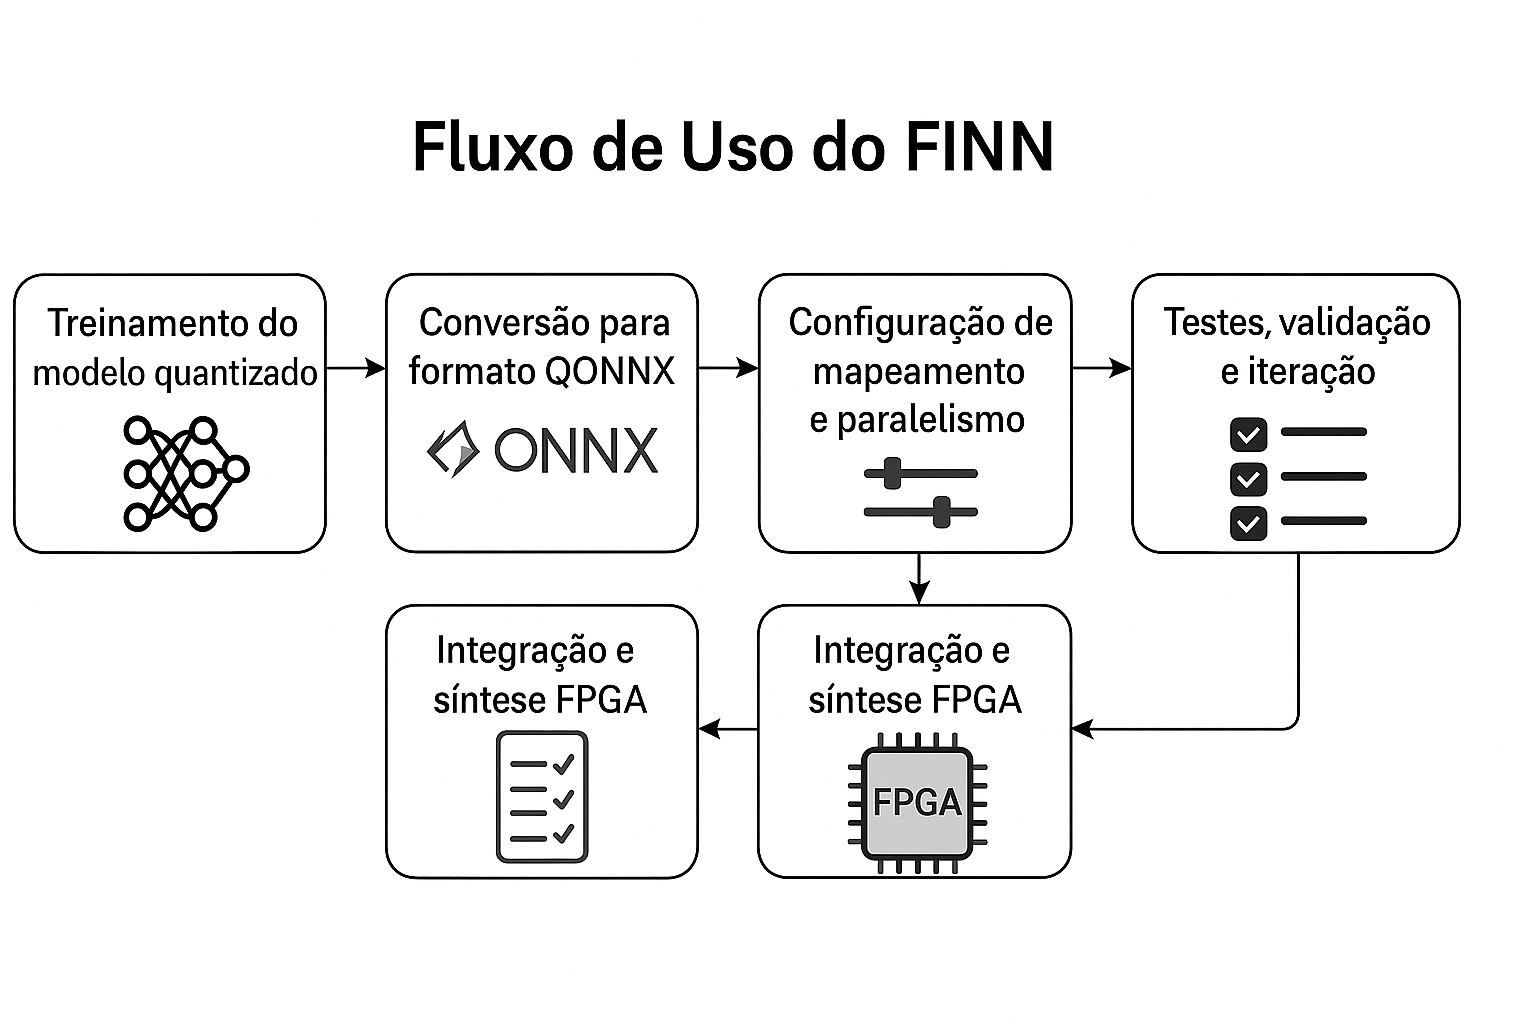
\includegraphics[width=0.80\linewidth]{FluxoUsoFINN.png}
%    \caption{Fluxo do uso do FINN. \\ Fonte: O autor.}
%    \label{fig:FINN_FluxoGeral}
%\end{figure}
%
%O processo se inicia com o \textbf{treinamento de um modelo quantizado}, normalmente conduzido no ambiente \textit{Brevitas}, onde pesos e ativações são ajustados para operar com baixa precisão (por exemplo, 1, 2, 4 ou 8 bits), mantendo a acurácia dentro de margens aceitáveis. Em seguida, o modelo é exportado no formato \textbf{QONNX} (\textit{Quantized Open Neural Network Exchange}), que atua como uma representação intermediária padronizada para a interoperabilidade entre frameworks de aprendizado e \mbox{ferramentas de síntese de hardware.}
%
%Na sequência, o usuário define os parâmetros de \textbf{mapeamento e paralelismo}, determinando a quantidade de unidades de computação, a profundidade de pipeline e o balanceamento entre latência e throughput. O \textbf{FINN Compiler} então converte o modelo quantizado em uma estrutura de hardware equivalente, gerando módulos em HLS ou RTL que representam cada camada da rede neural. Esses módulos são organizados em um fluxo contínuo de dados (\textit{dataflow architecture}), no qual as saídas de uma camada são transmitidas diretamente para a próxima, minimizando a necessidade \mbox{de armazenamento intermediário.}
%
%Após a \textbf{geração dos IPs} (blocos de hardware), o projeto é integrado em ambiente de síntese como o \textit{Vivado} ou o \textit{Vitis}, com conexão via barramento AXI e lógica de controle personalizada. A partir dessa integração, realiza-se a síntese, implementação e geração do \textbf{bitstream}, que configura o FPGA conforme o design projetado.
%
%Finalmente, a etapa de \textbf{teste e validação} avalia o desempenho real do sistema em termos de utilização de recursos, latência, consumo energético e acurácia. Esse processo é iterativo — ajustes finos podem ser aplicados para otimizar o desempenho, explorar paralelismo adicional ou adaptar o hardware a diferentes topologias de rede.
%
%Assim, o diagrama sintetiza o papel do FINN como um elo entre o domínio do aprendizado profundo e o projeto digital reconfigurável, demonstrando como a abstração de alto nível pode ser convertida, de forma automatizada e eficiente, em uma arquitetura física otimizada para execução em FPGA.
%
%
%O FINN também possui extensões importantes, como o \textbf{FINN-R}, um fluxo \textit{end-to-end} de exploração de espaço de design (\textit{Design Space Exploration}) que automatiza a análise de \textit{trade-offs} entre desempenho, consumo e área de hardware, gerando configurações otimizadas de aceleradores personalizados.
%
%Considerando sua capacidade de paralelismo massivo, determinismo temporal e eficiência energética, o FINN consolida-se como uma ferramenta de destaque para a execução de algoritmos de aprendizado profundo em tempo real. Essas características o tornam especialmente adequado para aplicações industriais e embarcadas, nas quais a confiabilidade, a baixa latência e a integração direta com sensores são requisitos fundamentais. Assim, compreender o fluxo de uso do FINN e sua arquitetura interna constitui um passo essencial para o desenvolvimento de sistemas inteligentes de monitoramento e diagnóstico baseados em FPGA.
%
%
%Na subseção seguinte, são apresentados estudos e trabalhos recentes que exploram o uso de FPGAs na aceleração de redes neurais e em aplicações de aprendizado de máquina, evidenciando o estado da arte e as tendências atuais dessa tecnologia no contexto da Inteligência Artificial embarcada.

%\subsection{Aplicações Recentes de FPGAs em Aprendizado de Máquina}
%
%\textcolor{red}{Ainda estou selecionado/lendo/resumindo os artigos}

\chapter{Metodologia}
% \section{Materiais e Métodos}
A metodologia adotada neste trabalho foi estruturada com base no modelo de \textit{Descoberta de Conhecimento em Bancos de Dados} (DCBD), proposto por Fayyad, Piatetsky-Shapiro e Smyth (1996). Esse modelo estabelece um ciclo sistemático de etapas voltadas à extração de conhecimento útil a partir de grandes volumes de dados, compreendendo as fases de seleção, pré-processamento, transformação, mineração e interpretação dos resultados.

No contexto deste projeto, o modelo DCBD foi adaptado para a realidade do monitoramento de sinais de emissão acústica, de forma que cada etapa corresponde a um processo específico dentro do desenvolvimento do sistema:
\begin{itemize}
    \item \textbf{Seleção:} coleta e organização dos sinais provenientes de ensaios experimentais e simulações;
    \item \textbf{Transformação:} conversão, segmentação e filtragem dos sinais brutos, preparando-os para análise;
    \item \textbf{Mineração:} aplicação de algoritmos de aprendizado de máquina, especialmente redes neurais convolucionais 1D, para identificação de padrões associados à cavitação e falhas incipientes;
    \item \textbf{Descoberta de conhecimento:} interpretação dos resultados e extração de informações relevantes para diagnóstico e manutenção preditiva.
\end{itemize}

Os materiais e ferramentas empregados abrangem tanto os recursos de hardware quanto de software indispensáveis para o desenvolvimento, teste e validação do sistema, incluindo plataformas FPGA, bibliotecas de aprendizado de máquina, e bases de dados de emissão acústica obtidas em bancada e em campo.

Para fins de organização, a metodologia foi estruturada em duas frentes complementares:
\begin{itemize}
    \item \textbf{Métodos de Desenvolvimento} — englobam o projeto e implementação dos módulos de aquisição, pré-processamento e análise de dados, bem como o fluxo de inferência em FPGA.
    \item \textbf{Métodos de Avaliação} — abrangem os procedimentos experimentais de validação, incluindo testes de desempenho, análise de acurácia e robustez do modelo proposto.
\end{itemize}

Essa divisão permite que a pesquisa mantenha um equilíbrio entre os aspectos teóricos e práticos do problema, assegurando tanto a viabilidade de implementação do sistema quanto a confiabilidade dos resultados obtidos.

\subsection*{Bases de Dados}

A etapa de formação da base de dados é essencial para o desenvolvimento e validação dos modelos de aprendizado de máquina aplicados à detecção de cavitação e falhas mecânicas. Neste trabalho, serão utilizadas três fontes de dados complementares, abrangendo diferentes tipos de sinais, condições de operação e contextos experimentais, conforme descrito a seguir:

\begin{itemize}
    \item \textbf{Falhas em Rolamentos — Case Western Reserve University (CWRU):}  
    Conjunto amplamente reconhecido na literatura de diagnóstico de falhas mecânicas, contendo medições de vibração adquiridas sob diferentes condições de carga e níveis de dano. Essa base é utilizada como referência para validação comparativa dos algoritmos de aprendizado supervisionado, permitindo aferir a capacidade de generalização do modelo.  
    \textit{Disponível em:} \url{https://engineering.case.edu/bearingdatacenter/download-data-file}

    \item \textbf{Cavitação em Bombas — UWA System Health Lab:}  
    Proveniente da \textit{Prognostics Data Library}, essa base inclui sinais acústicos registrados durante ensaios controlados de cavitação em bombas centrífugas, com variáveis de operação conhecidas. É utilizada para calibrar o modelo de classificação e investigar o comportamento espectral característico da cavitação em diferentes regimes de escoamento.  
    \textit{Disponível em:} \url{https://systemhealthlab.com/research-tools/prognostics-data-library}

    \item \textbf{Bancada Experimental — Projeto MOMEA (Itaipu Binacional / ParqueTec):}  
    Conjunto de dados obtido em bancada desenvolvida no âmbito do projeto MOMEA, composta por motobombas instrumentadas com sensores de Emissão Acústica (EA) e vibração. Os ensaios permitem registrar eventos reais de cavitação e anomalias estruturais sob condições de operação controladas, sendo a principal fonte de dados para validação do sistema proposto em ambiente físico.
\end{itemize}

A combinação dessas três bases — pública, controlada e experimental — possibilita uma avaliação abrangente do modelo, tanto em termos de robustez quanto de aplicabilidade prática, assegurando diversidade de amostras e condições de ruído representativas de cenários industriais reais.

\subsection*{Softwares e Ferramentas}

O desenvolvimento do sistema proposto envolve a integração de ferramentas de software e plataformas de hardware voltadas à síntese, simulação e validação em FPGA. A seguir, apresentam-se os principais recursos tecnológicos empregados:

\begin{itemize}
    \item \textbf{FINN Framework:}  
    Framework de código aberto desenvolvido pela Xilinx/AMD Research para aceleração de redes neurais quantizadas (\textit{Quantized Neural Networks — QNNs}) em FPGAs. O FINN permite converter modelos treinados em PyTorch (via Brevitas) em arquiteturas de fluxo de dados altamente otimizadas, com geração automática de IPs em HLS/RTL. Essa ferramenta constitui a base do fluxo de inferência embarcado adotado neste projeto.

    \item \textbf{Vivado Design Suite:}  
    Ambiente oficial da Xilinx para síntese e implementação de sistemas digitais em HDL (VHDL/Verilog) ou alto nível (C/C++/OpenCL via HLS). É utilizado para o mapeamento físico do hardware, análise de temporização, integração de IPs e geração do \textit{bitstream} final que configura o FPGA.

    \item \textbf{Plataformas FPGA:}  
    Serão utilizados, em etapas progressivas de desenvolvimento, os dispositivos \textit{Artix-7 35T} (Xilinx) e uma segunda placa de maior capacidade (a confirmar, sob orientação do Prof. Márcio). A escolha definitiva considerará a disponibilidade de blocos DSP, BRAM e recursos lógicos necessários para a execução da CNN quantizada e dos módulos de comunicação.
\end{itemize}

O uso combinado dessas ferramentas permite transpor o modelo de aprendizado de máquina do domínio de software para uma implementação física eficiente, explorando o paralelismo e a reconfigurabilidade inerentes aos FPGAs para alcançar baixa latência e alta confiabilidade operacional.

\subsection*{Métodos de Desenvolvimento}

Esta subseção descreve as etapas e procedimentos adotados para o desenvolvimento do sistema de aquisição, processamento e análise dos sinais de emissão acústica, bem como a implementação dos algoritmos de aprendizado de máquina e sua integração em FPGA. O foco está em detalhar o fluxo de concepção técnica, desde a captura dos dados experimentais até o mapeamento do modelo neural no hardware reconfigurável.

O desenvolvimento foi conduzido de forma modular, abrangendo três eixos principais:
\begin{enumerate}
    \item \textbf{Aquisição e Pré-processamento de Dados:} construção da base de dados de emissão acústica e implementação de técnicas de filtragem e normalização dos sinais;
    \item \textbf{Modelagem e Treinamento:} aplicação de redes neurais convolucionais unidimensionais (CNN~1D) para detecção e classificação de padrões acústicos associados à cavitação;
    \item \textbf{Implementação em FPGA:} conversão do modelo treinado para formato quantizado e síntese via framework FINN, permitindo execução embarcada em tempo real.
\end{enumerate}

O objetivo desta etapa metodológica é garantir um pipeline eficiente, reprodutível e otimizado tanto em termos computacionais quanto de desempenho físico, assegurando a viabilidade da aplicação industrial do sistema proposto.

\subsection*{Métodos de Avaliação}

Nesta subseção, são apresentados os procedimentos adotados para a validação experimental e análise de desempenho do sistema proposto. As avaliações foram conduzidas em dois níveis complementares: desempenho funcional do modelo de aprendizado de máquina e desempenho operacional da implementação em FPGA.

O primeiro nível de avaliação contempla métricas clássicas de aprendizado supervisionado — como acurácia, precisão, sensibilidade, especificidade e matriz de confusão — aplicadas aos resultados de classificação obtidos pela CNN~1D. Já o segundo nível foca em métricas de engenharia de hardware, incluindo utilização de recursos lógicos (LUTs, flip-flops, DSPs, BRAMs), consumo de energia, latência de inferência e throughput.

Adicionalmente, os experimentos de validação foram realizados com base em dados reais de emissão acústica provenientes de ensaios de bancada e simulações controladas de cavitação, de modo a avaliar a robustez e generalização do modelo em diferentes condições de operação.

Esses métodos de avaliação permitem correlacionar diretamente o desempenho do algoritmo com sua eficiência no hardware, oferecendo uma visão integrada do potencial do sistema para aplicações de monitoramento preditivo e diagnóstico inteligente em máquinas rotativas.

% \section{Métodos de Desenvolvimento}
% \section{Métodos de Avaliação}

\chapter{Resultados parciais}
\section{MomeaProbe/MomeaCapture: Captura continua de dados}

No escopo do Projeto \textbf{MOMEA — Monitoramento Online de Rotores de Turbinas pelo Método de Emissão Acústica}, desenvolvido pelo grupo de pesquisa da Itaipu ParqueTec em parceria com a Itaipu Binacional, foram implementadas aplicações experimentais voltadas à análise de sinais acústicos e vibromecânicos obtidos de motobombas submetidas a diferentes condições de operação.  

O sistema \textbf{MomeaProbe/MomeaCapture} atua como plataforma de aquisição de dados, realizando a captura simultânea de sinais de Emissão Acústica (EA), vibração e/ou pressão em alta taxa de amostragem. O MomeaProbe é o hardware composto por dois ADCs de 12 bits operando a 8Msps e transmissão via interface USB~3.0, a placa e como mostrada na Figura ~\ref{fig:MomeaProbe12USB}.

\begin{figure}[H]
    \centering
    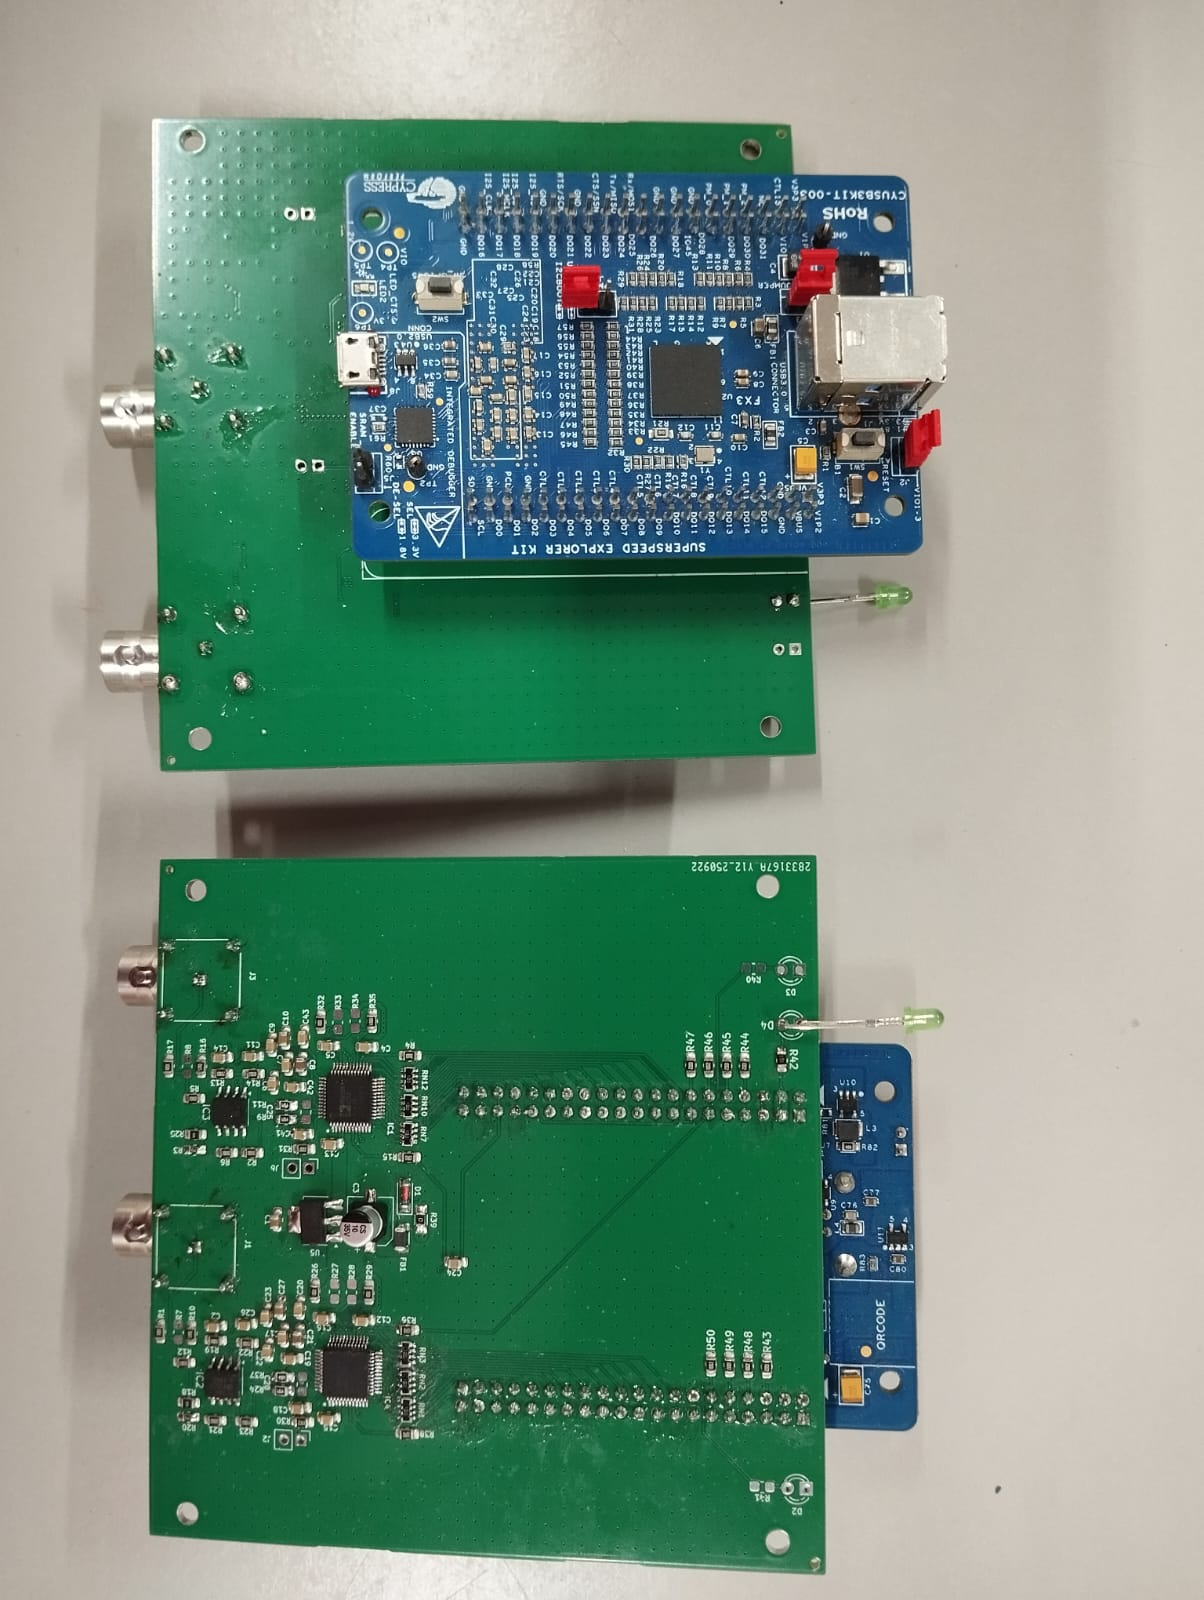
\includegraphics[width=0.5\linewidth, angle=90]{figs/PlacasADC_AD9226.jpeg}
    \caption{Placas de captura de sinais MomeaProbe12USB}
    \label{fig:MomeaProbe12USB}
\end{figure}

Os dados adquiridos no ambiente \textbf{MomeaCapture}, Figura ~\ref{fig:MomeaCapture}, uma aplicação desenvolvida em C++/Qt, responsável pelo gerenciamento da transferência, compressão, armazenamento e visualização dos sinais. Essa arquitetura possibilita o registro contínuo de longas séries temporais com resolução temporal suficiente para a análise espectral de fenômenos de cavitação e microfalhas estruturais.

\begin{figure}[H]
    \centering
    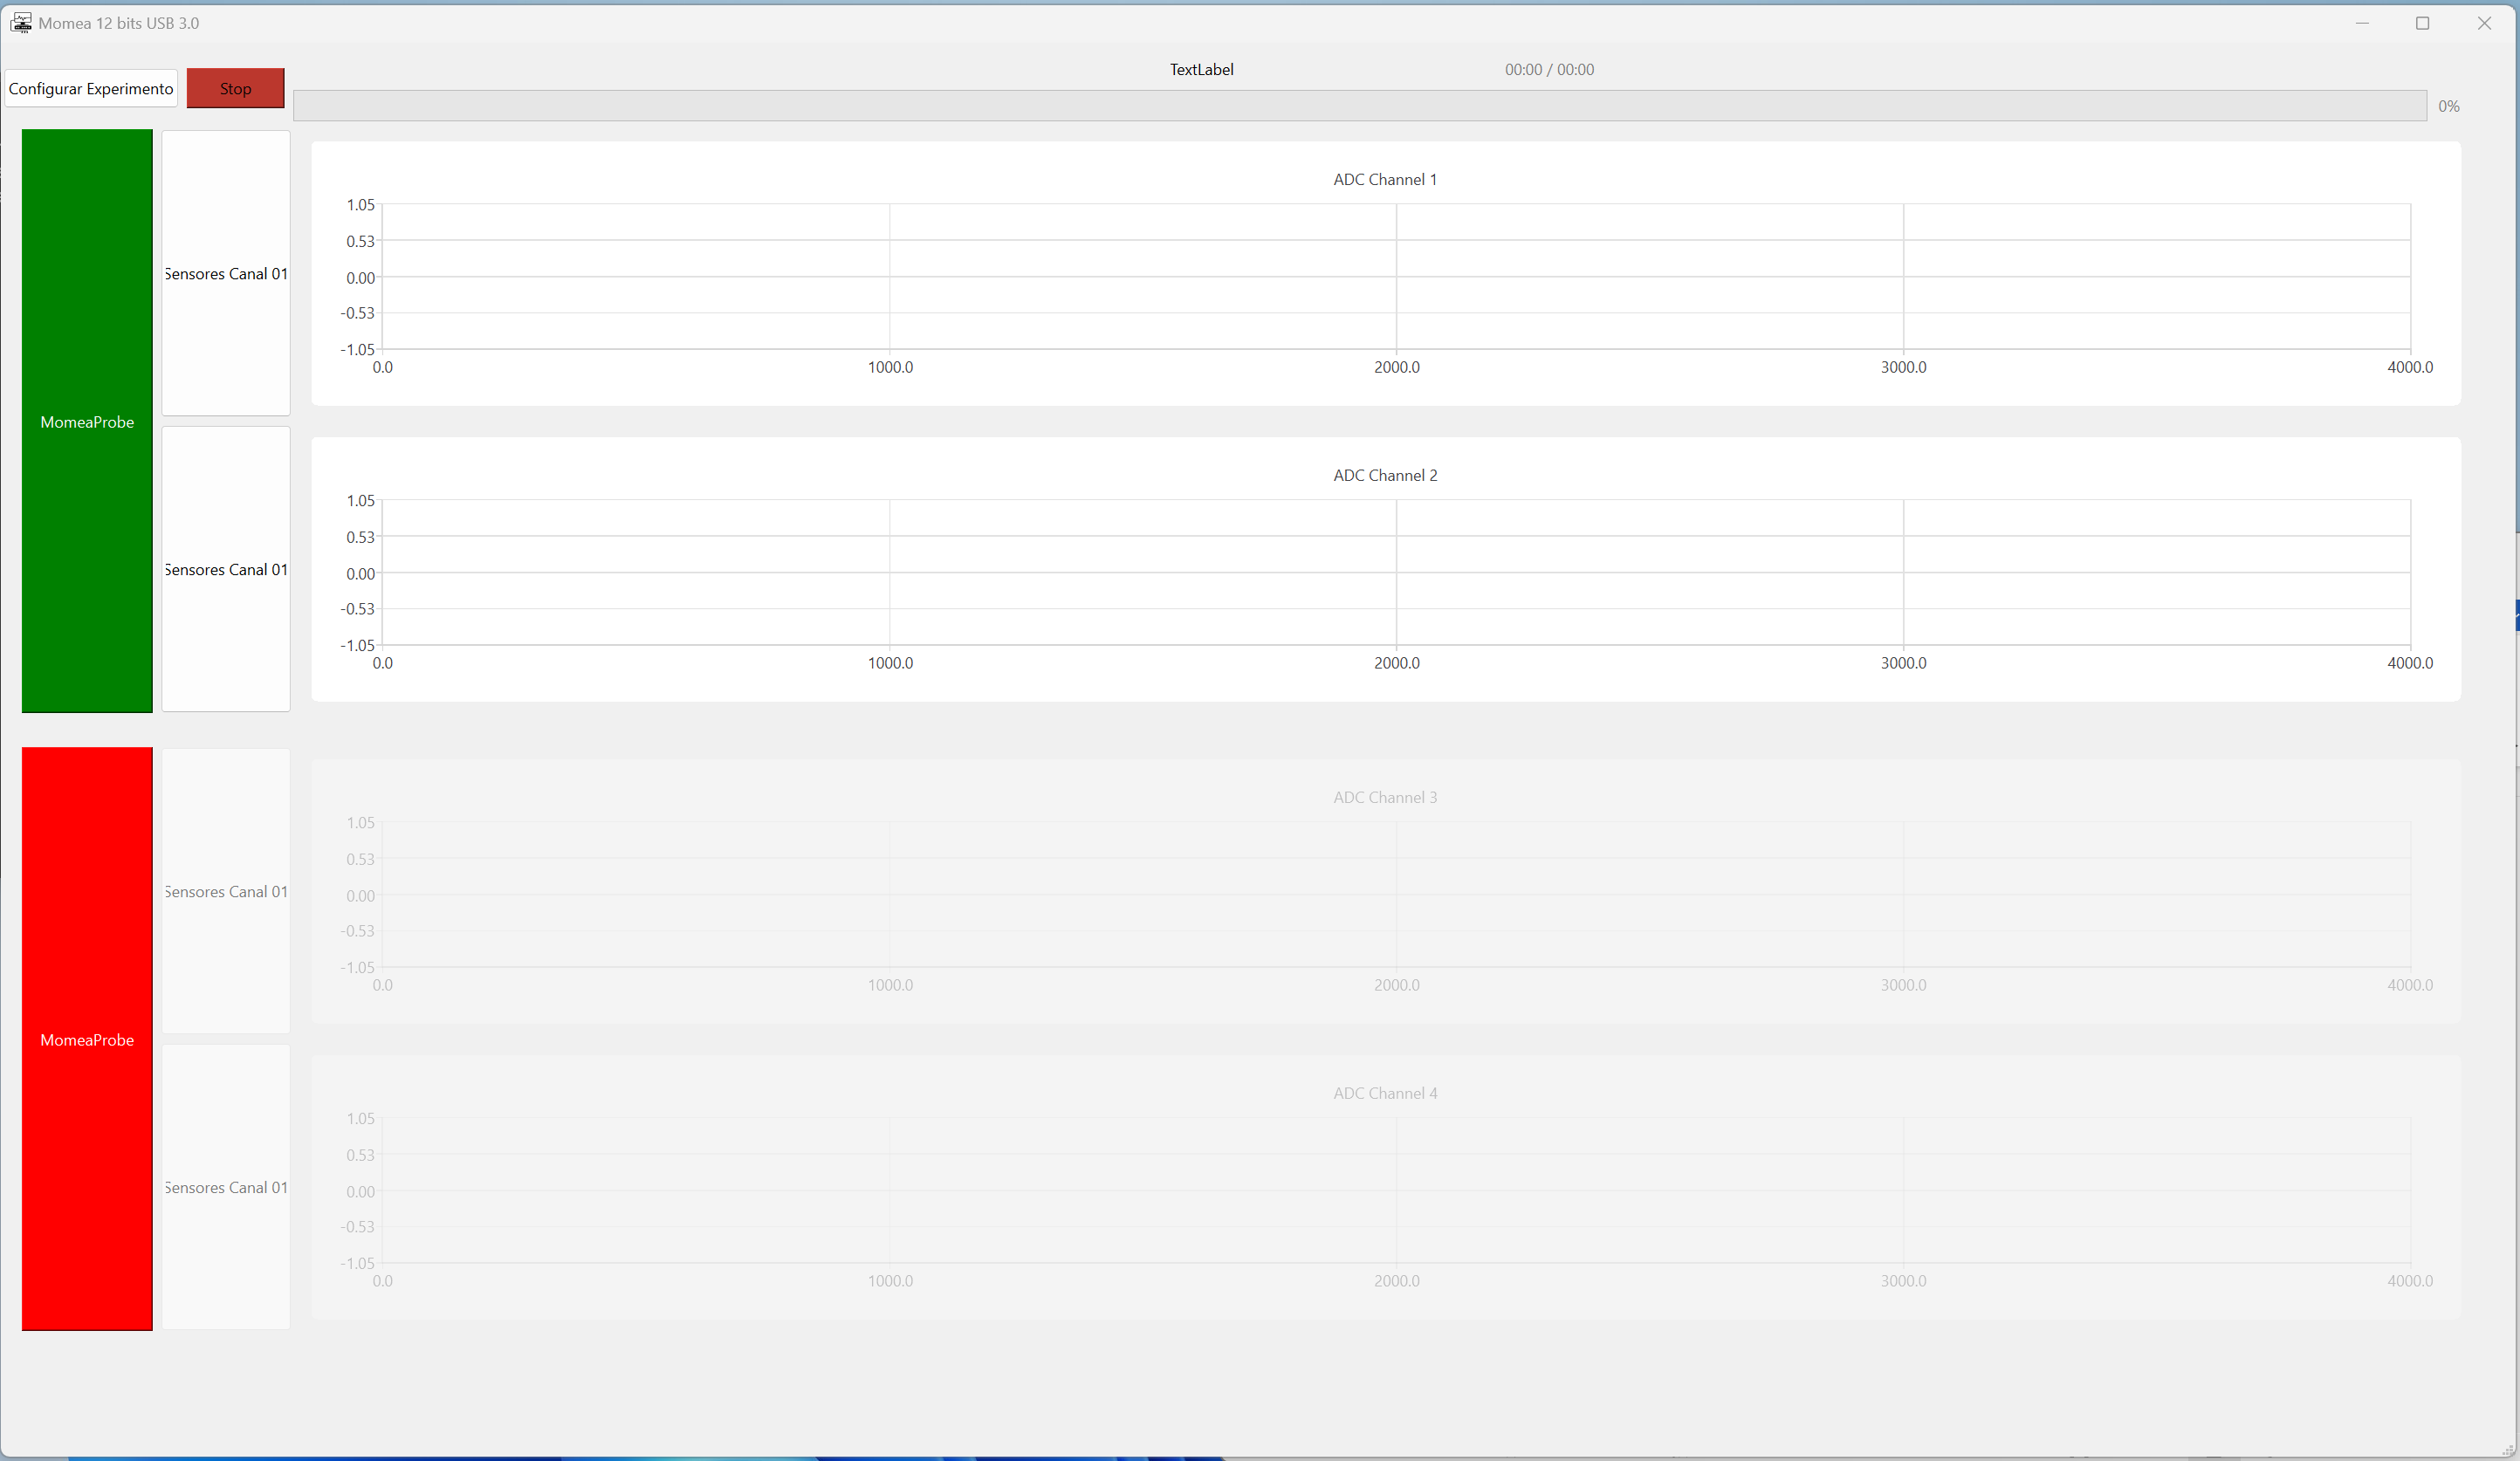
\includegraphics[width=0.5\linewidth]{figs/MomeaCapture.png}
    \caption{Software de captura MomeaCapture}
    \label{fig:MomeaCapture}
\end{figure}

Para a análise no domínio da frequência, foi implementado um módulo de processamento baseado na \textbf{Transformada Rápida de Fourier (FFT)} com janelamento móvel (\textit{short-time FFT}). Essa abordagem permite gerar imagens do espectro de frequência em função do tempo, produzindo mapas espectro-temporais semelhantes a espectrogramas. As imagens resultantes evidenciam o comportamento dinâmico dos componentes de alta frequência associados a eventos de cavitação, facilitando sua visualização e posterior interpretação automática.

A partir desses espectrogramas, foram treinadas redes neurais convolucionais bidimensionais (\textbf{CNN 2D}) — tradicionalmente empregadas em processamento de imagens — para identificar padrões característicos de cavitação em bombas centrífugas. O uso de CNNs 2D mostrou-se eficaz para distinguir condições normais, de cavitação incipiente e cavitação plenamente desenvolvida, aproveitando as propriedades espaciais e frequenciais extraídas das janelas espectrais.

Apesar dos resultados promissores, essa abordagem apresenta limitações inerentes ao grande volume de dados gerado e armazenado. O sistema MomeaProbe pode produzir dezenas de gigabytes por hora de operação contínua, o que é vantajoso durante a fase de treinamento dos modelos, mas inviável para o monitoramento em tempo real devido ao alto custo computacional e à latência de processamento. A geração de espectrogramas e a inferência em CNNs 2D exigem processamento intensivo, tornando o sistema dependente de GPU ou CPU de alto desempenho para alcançar taxas adequadas de atualização.

Diante dessas restrições, está em desenvolvimento uma solução baseada em \textbf{arquitetura FPGA-HIT (Hardware-in-the-Loop com Inferência Temporal)}, voltada à execução direta de inferência em tempo real no hardware reconfigurável. Essa nova abordagem, que será detalhada na próxima subseção, visa reduzir drasticamente a latência e o consumo de energia, mantendo a precisão do modelo por meio da quantização e otimização do pipeline de inferência embarcado.

\section{FPGA e Técnica de HIT}

Baseado na metodologia de detecção por \textbf{HIT (Hit Detection)}, descrita anteriormente na Seção~\ref{sec:UsoEA}, está em desenvolvimento uma implementação dedicada em \textbf{FPGA}, com o objetivo de realizar o pré-processamento e a filtragem dos sinais de Emissão Acústica (EA) diretamente no hardware, reduzindo significativamente o volume de dados a serem transmitidos e processados posteriormente no sistema de monitoramento.

A plataforma selecionada para essa implementação é a \textbf{Arty A7-35T}, da Digilent, mostrada na Figura \ref{fig:Arty} equipada com o \textbf{FPGA Xilinx Artix-7 XC7A35T}. Esse dispositivo conta com aproximadamente 33.280 células lógicas, 1.800~kB de memória interna distribuída (Block RAM), 90 blocos DSP~(Digital Signal Processing) e interfaces externas configuráveis. O Artix-7 oferece excelente equilíbrio entre custo, consumo energético e capacidade de processamento paralelo, sendo ideal para aplicações de prototipagem de sistemas embarcados de processamento em tempo real.

\begin{figure}[H]
    \centering
    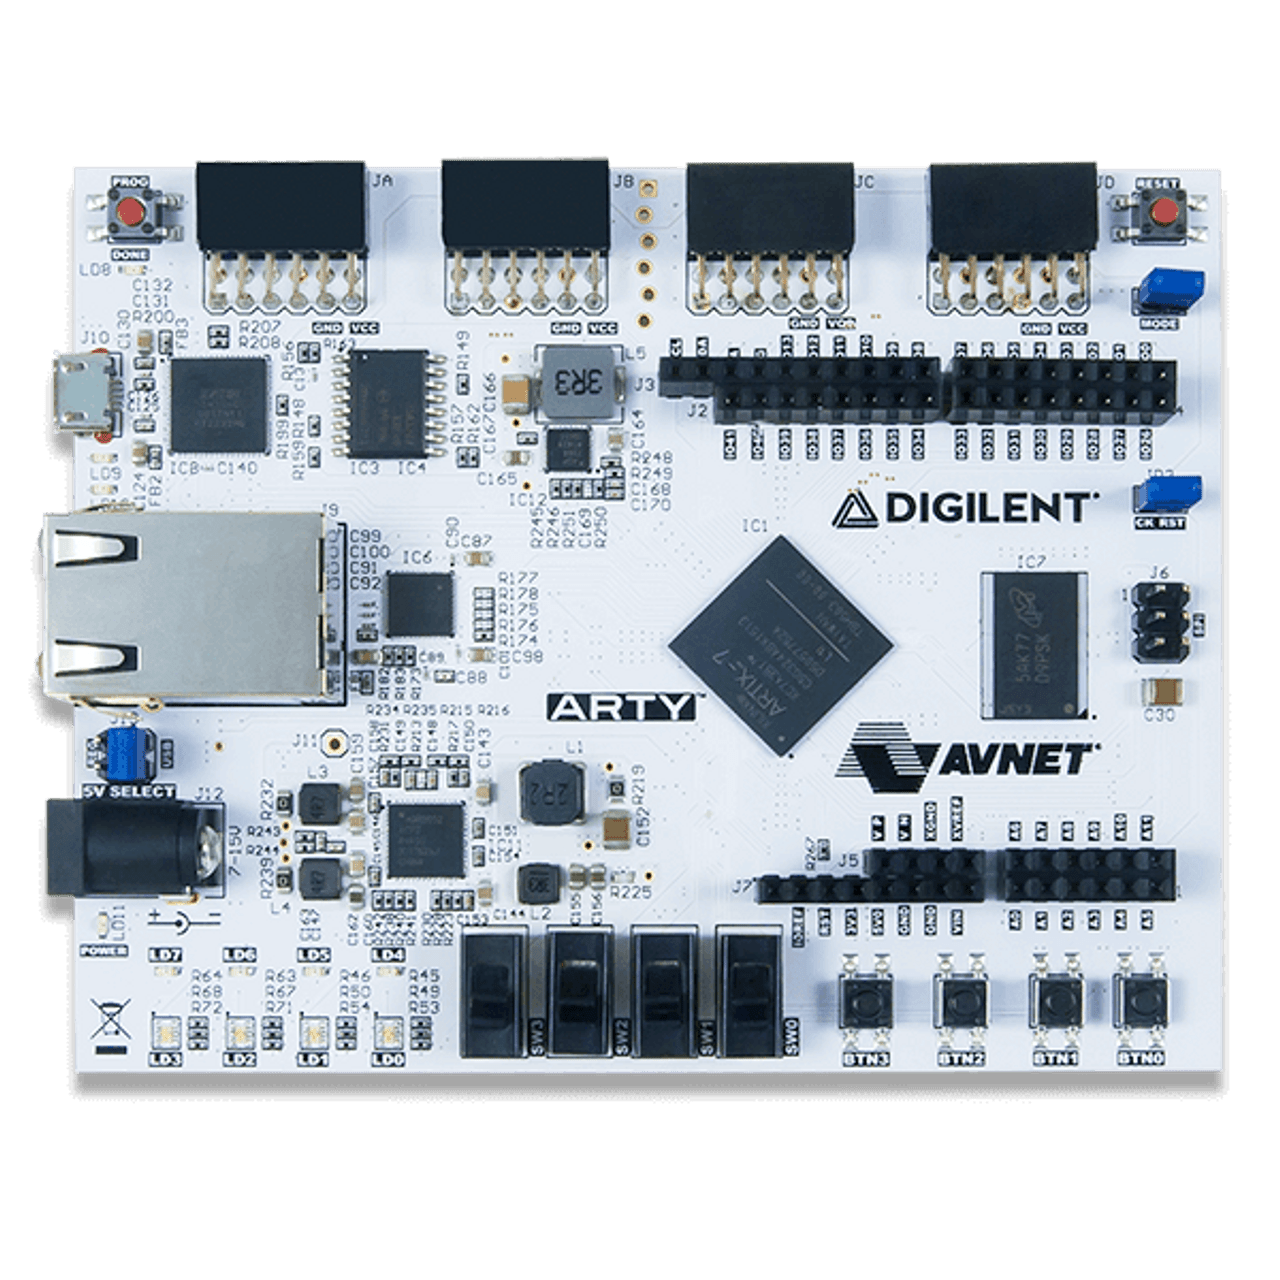
\includegraphics[width=0.5\linewidth]{figs/Arty_top.png}
    \caption{Placa de desenvolvimento Arty A7 35T.}
    \label{fig:Arty}
\end{figure}

Na arquitetura proposta, o FPGA executa o processamento de eventos de Emissão Acústica a partir da técnica de \textbf{detecção de HIT}, a qual identifica e caracteriza apenas os trechos do sinal que ultrapassam limiares definidos de amplitude ou energia. Esse método, conforme discutido na fundamentação teórica, permite registrar parâmetros essenciais de cada evento — como amplitude máxima, duração, energia e tempo de ocorrência — em vez de armazenar o sinal completo. Dessa forma, o volume de dados é reduzido em várias ordens de magnitude, o que viabiliza o monitoramento contínuo de longo prazo sem sobrecarregar a comunicação nem o armazenamento.

A implementação faz uso de uma \textbf{Soft CPU MicroBlaze}, processador configurável integrado ao FPGA e responsável pelo controle das tarefas de comunicação e gerenciamento do sistema. Sobre essa CPU, é executado o sistema operacional \textbf{FreeRTOS}, que permite o agendamento de múltiplas tarefas de forma determinística e de baixa latência, garantindo sincronismo entre a lógica de detecção de eventos e as rotinas de transmissão de dados.

A comunicação entre o módulo FPGA e o sistema de supervisão é realizada por meio de uma interface \textbf{Ethernet 10/100~Mbps}, implementada via controlador MAC interno e pilha TCP/IP embarcada. Esse canal é utilizado tanto para o envio dos eventos detectados quanto para o recebimento de comandos de configuração, como atualização de limiares, modos de operação e parâmetros de calibração.

Devido à natureza esparsa dos sinais de Emissão Acústica — em que longos períodos de silêncio são interrompidos por breves eventos de alta energia —, a técnica de HIT proporciona uma drástica redução no volume de dados transmitidos. Durante o regime normal de operação, em que não há eventos significativos, o tráfego de dados é mínimo. Mesmo durante a ocorrência de múltiplos eventos, a quantidade de informação permanece controlada, uma vez que apenas os descritores compactos de cada HIT são enviados.

Essa abordagem híbrida, combinando \textbf{processamento distribuído em hardware} e \textbf{controle multitarefa em software embarcado}, representa um avanço significativo rumo à \textbf{plataforma MOMEA-FPGA-HIT}, cuja meta é realizar a detecção de falhas em tempo real, com baixo consumo, alta confiabilidade e escalabilidade para integração em sistemas industriais. Os resultados preliminares indicam que essa arquitetura é capaz de reduzir substancialmente a latência de detecção e o volume de dados, mantendo a sensibilidade necessária para identificar fenômenos de cavitação e microtrincas em rotores de motobombas.

\subsection{Limitações do Método de HIT em Relação a Técnicas Baseadas em Aprendizado de Máquina}

Embora a técnica de detecção de eventos por \textbf{HIT} apresente vantagens significativas em termos de simplicidade, baixo custo computacional e eficiência no uso de memória, ela também possui limitações importantes quando comparada a abordagens baseadas em \textbf{aprendizado de máquina}, especialmente redes neurais convolucionais (\textit{Convolutional Neural Networks — CNNs}) e suas variantes unidimensionais (\textit{CNN-1D}).

A principal limitação do método de HIT reside no fato de que sua operação depende fortemente da definição de \textbf{limiares de detecção} (thresholds). Esses limiares são utilizados para identificar o instante em que a amplitude do sinal de Emissão Acústica (EA) ultrapassa um valor pré-determinado, indicando a ocorrência de um evento. No entanto, limiares mal ajustados podem levar a dois problemas críticos:

\begin{itemize}
    \item \textbf{Perda de eventos relevantes:}  
    Eventos de baixa amplitude — frequentemente associados a fenômenos incipientes, como o início da cavitação ou a formação de microtrincas — podem não ultrapassar o limiar definido e, portanto, não ser registrados. Essa limitação compromete a sensibilidade do sistema em detectar falhas em estágios iniciais.

    \item \textbf{Falsos negativos e dependência de calibração:}  
    O desempenho do método depende fortemente da calibração experimental, que pode variar conforme o tipo de sensor, o acoplamento mecânico, o ruído estrutural e as condições de operação da máquina. Pequenas variações nessas condições podem alterar significativamente a amplitude dos sinais, exigindo reconfigurações frequentes dos parâmetros de detecção.
\end{itemize}

Além disso, o método de HIT não considera a \textbf{estrutura temporal e espectral completa} do sinal, pois registra apenas parâmetros estatísticos resumidos — como amplitude máxima, duração, energia e número de contagens — sem preservar a forma de onda original. Isso limita a capacidade do sistema de capturar padrões complexos ou sutis que poderiam ser indicativos de processos físicos distintos, como cavitação transitória, impactos mecânicos ou ruídos estruturais.

Em contraste, modelos de aprendizado profundo, como as \textbf{CNNs 2D} e \textbf{CNN-1D}, analisam diretamente os sinais brutos ou suas representações espectro-temporais, aprendendo automaticamente características discriminativas que podem não ser evidentes a partir de parâmetros manuais. Essas redes são capazes de detectar relações não lineares, correlações temporais e variações espectrais de pequena magnitude, o que as torna particularmente eficazes para identificar estágios iniciais de cavitação ou falhas de natureza intermitente.

Por fim, embora o método de HIT seja extremamente eficiente para \textbf{monitoramento contínuo embarcado}, ele se mostra limitado em cenários que demandam \textbf{diagnóstico detalhado ou classificação precisa de eventos}. Assim, uma solução híbrida — na qual a detecção inicial por HIT seja complementada por um módulo de inferência baseado em CNN embarcado em FPGA — surge como uma alternativa promissora, combinando a eficiência do pré-processamento em hardware com o poder discriminativo do aprendizado profundo.

\section{Resultados Parciais e Proposta de Pesquisa}

Os resultados obtidos até o momento demonstram a viabilidade da detecção de cavitação em bombas centrífugas por meio da análise espectro-temporal de sinais acústicos, utilizando redes neurais convolucionais (\textbf{CNNs}) aplicadas a imagens de espectrogramas geradas a partir da Transformada Rápida de Fourier (FFT) janelada. Essa abordagem, implementada no ambiente de software \textbf{MomeaCapture}, tem se mostrado eficaz para classificar diferentes estágios de cavitação e distinguir condições de operação normais, incipientes e severas. No entanto, sua principal limitação reside no elevado volume de dados processados e na latência associada ao fluxo contínuo de aquisição via USB~3.0, o que restringe sua aplicação em monitoramento em tempo real.

Para superar essas limitações, propõe-se o estudo e a simulação de uma arquitetura embarcada de \textbf{inferência em FPGA}, baseada em uma rede \textbf{CNN-1D} otimizada e quantizada. Essa proposta busca unir o poder discriminativo das redes neurais convolucionais — capazes de identificar padrões sutis e não lineares mesmo em sinais compactados — com a eficiência e o paralelismo inerentes ao hardware reconfigurável. O objetivo é possibilitar o \textbf{processamento em tempo quase real} (\textit{near real-time}) diretamente no dispositivo, reduzindo significativamente a latência e o volume de dados transmitidos, de modo que apenas alertas de falhas ou eventos relevantes sejam enviados ao sistema de monitoramento superior.

% A comparação entre as duas abordagens pode ser sintetizada da seguinte forma:

% \begin{table}[H]
% \centering
% \caption{Comparação entre os métodos contínuo (USB + CNN 2D) e embarcado (FPGA + HIT + CNN 1D).}
% \label{tab:comparacao_usb_fpga}
% \renewcommand{\arraystretch}{1.3}
% \resizebox{\textwidth}{!}{
% \begin{tabular}{p{4.2cm} p{5.3cm} p{5.3cm}}
% \hline
% \textbf{Aspecto} & \textbf{Método Contínuo (USB + CNN 2D)} & \textbf{Método Embarcado (FPGA + HIT + CNN 1D)} \\ \hline
% \textbf{Aquisição de Dados} & Fluxo contínuo via USB~3.0 (40~Msps por canal) & Aquisição seletiva por eventos (HITs) via ADC interno \\ \hline
% \textbf{Pré-processamento} & FFT janelada e geração de espectrogramas & Detecção de HIT e extração de parâmetros compactos \\ \hline
% \textbf{Modelo de IA} & CNN 2D aplicada a imagens espectro-temporais & CNN 1D aplicada a trechos de sinal compactado \\ \hline
% \textbf{Volume de Dados} & Elevado — dezenas de GB/hora & Reduzido — apenas eventos relevantes \\ \hline
% \textbf{Latência de Processamento} & Alta — dependente de GPU/CPU & Baixa — inferência em hardware dedicada \\ \hline
% \textbf{Consumo de Energia} & Alto (processamento contínuo) & Baixo (ativação sob demanda) \\ \hline
% \textbf{Aplicação Ideal} & Treinamento e análise off-line & Monitoramento contínuo embarcado em campo \\ \hline
% \end{tabular}}
% \end{table}

% Com base nesses resultados e na análise comparativa apresentada, o desenvolvimento do sistema \textbf{FPGA + HIT + CNN-1D} representa o próximo passo natural do projeto MOMEA. Essa solução busca aliar a precisão do aprendizado profundo à eficiência da computação reconfigurável, estabelecendo as bases para uma plataforma de \textbf{monitoramento inteligente em tempo real} capaz de detectar cavitação e falhas incipientes com alta sensibilidade e confiabilidade, diretamente no ambiente industrial.


% \chapter{Conclusão}
%% \chapter{Introdução}
% \section{Formulação do Problema}
% A detecção precoce de falhas em equipamentos industriais é essencial para a manutenção da integridade estrutural e o prolongamento da vida útil de componentes mecânicos, reduzindo custos operacionais e evitando paradas inesperadas. Entre os diversos tipo de equipamentos as Bombas hidráulicas são amplamente utilizadas na indústria e na vida diária como um tipo de maquinário de fluidos. Elas são usadas para fornecer a energia necessária para transferir fluidos. Entre os fenômenos que afetam a eficiência e a segurança desses equipamentos, a cavitação em bombas centrífugas representa um desafio significativo, pois provoca erosões, trincas e desgastes superficiais, comprometendo o desempenho e a confiabilidade desses sistemas Várias falhas podem ocorrer durante a operação real. Em geral, a cavitação ocorre quando a pressão estática em algum ponto dentro de uma bomba é menor do que a pressão de vapor do líquido na temperatura de trabalho. Nesse caso, um grande número de bolhas é criado, e essas bolhas entrarão em colapso quando o líquido atingir a zona de alta pressão. Uma vez que a cavitação ocorre, a troca de energia entre o impulsor e o fluido é danificada, a curva de vazão cai e a superfície das peças de passagem do fluxo é severamente desgastada e corroída . Além disso, causará ruído e vibração do corpo da bomba. Portanto, a cavitação é uma questão científica significativa no campo de bombas e um ponto de preocupação atual. A detecção de cavitação se tornou um problema urgente a ser resolvido, o que tem uma importância muito importante em termos de segurança e economia \cite{liu2023review}.


% \section{Motivação}
% O Projeto MOMEA, conduzido pela Itaipu Binacional, busca desenvolver soluções para o monitoramento inteligente da intensidade da cavitação e identificação de regiões propensas à formação de trincas nos rotores de turbinas, visando aprimorar a segurança e a eficiência de seus equipamentos. No entanto, sistemas tradicionais de monitoramento dependem de análises posteriores às inspeções físicas ou de métodos que exigem conhecimento especializado para a interpretação dos dados coletados. Nesse contexto, abordagens baseadas em aprendizado de máquina apresentam-se como uma solução promissora para a análise automatizada de sinais de sensores instalados em equipamentos industriais, permitindo a identificação de padrões anormais e a previsão de falhas antes que se tornem críticas \textcolor{red}{(SOUZA et al., 2022)}.


% \section{Justificativa}
% O método de detecção de falhas de cavitação baseado em sinal é baseado no fato de que o fenômeno de cavitação que o acompanha mudará os sinais acústicos, de vibração e de pulsação de pressão dentro da bomba. Há uma certa relação entre a mudança no sinal e a ocorrência de cavitação. Sensores de sinal são instalados em diferentes posições da bomba, coletando o sinal de dados no estado operacional da bomba para análise. Ao mesmo tempo, algoritmos de inteligência artificial, como aprendizado de máquina e aprendizado profundo, são usados para obter extração de características e reconhecimento de estado. O processo básico de detecção de falhas de cavitação é mostrado na Figura 1. Comparado com outros métodos de detecção, o método de detecção de cavitação baseado em diferentes sinais pode ser aplicado a sistemas complexos e não lineares e tem baixos requisitos do ambiente de campo. Ao mesmo tempo, os métodos de sinal são úteis para melhorar o desempenho do sistema de detecção. Portanto, os pesquisadores realizaram um extenso trabalho nesta área \cite{liu2023review}.


% Entretanto, a implementação de modelos de aprendizado de máquina em sistemas embarcados enfrenta desafios relacionados ao processamento de grandes volumes de dados em tempo real e ao consumo de energia. O uso de Field Programmable Gate Arrays (FPGAs) para a execução desses modelos pode superar essas limitações, pois oferece alto desempenho computacional, baixa latência e eficiência energética em comparação com soluções baseadas em CPUs ou GPUs.


% Diante desse contexto, surge a necessidade de desenvolver um modelo de aprendizado de máquina embarcado em FPGA capaz de classificar a intensidade da cavitação em bombas centrífugas, utilizando dados obtidos por sensores de Emissão Acústica (EA) e acelerômetros. O desafio central consiste em projetar um sistema eficiente, que possa processar os sinais em tempo real e fornecer diagnósticos precisos, contribuindo assim para a melhoria da manutenção preditiva e a otimização da operação de equipamentos industriais.


% \section{Contribuições}
% As possíveis contribuições deste projeto incluem o desenvolvimento de uma metodologia inovadora para a detecção e classificação da intensidade da cavitação em bombas centrífugas, permitindo a identificação precoce de falhas e a mitigação de danos estruturais. A utilização de aprendizado de máquina embarcado em FPGA possibilita a análise de sinais com pouco atraso em na identificação da ocorrência de um problema e sua detecção, reduzindo a dependência de inspeções físicas e facilitando a manutenção preditiva. Além disso, o projeto contribui para a otimização da operação de equipamentos industriais, aumentando sua eficiência e confiabilidade, ao mesmo tempo em que reduz custos operacionais e o consumo de energia. A implementação de sensores de Emissão Acústica (EA) e acelerômetros aprimora a precisão na detecção de padrões anômalos, proporcionando uma abordagem mais robusta para o monitoramento de bombas centrífugas. Adicionalmente, este estudo fortalece a aplicação de tecnologias de hardware reconfigurável para tarefas de inteligência artificial, demonstrando a viabilidade do uso de FPGAs para o processamento eficiente de grandes volumes de dados em sistemas embarcados industriais.
\section{Formulação do Problema}

A detecção em estágio inicial de falhas em equipamentos industriais revela-se essencial para assegurar a integridade estrutural dos ativos, prolongar a vida útil dos componentes mecânicos, reduzir os custos operacionais e prevenir paradas inesperadas. Dentre os diversos tipos de equipamentos, as bombas hidráulicas se sobressaem pela sua ampla utilização nos setores industriais e em aplicações cotidianas, desempenhando um papel central no transporte de fluidos.

No conjunto de fenômenos que comprometem a eficiência e a confiabilidade desses dispositivos, a cavitação em bombas centrífugas destaca-se como um desafio relevante. Este fenômeno induz erosão, trincas e desgaste superficial nos componentes, afetando o desempenho hidráulico e reduzindo a vida útil do sistema. A cavitação ocorre quando a pressão estática em uma determinada região da bomba cai abaixo da pressão de vapor do líquido na respectiva temperatura de operação. Nessa situação, formam-se bolhas de vapor que, ao migrarem para zonas de pressão mais elevada, colapsam com liberação de energia intensa, ocasionando impactos capazes de danificar o impulsor e provocar a degradação da curva característica de vazão.

Além dos danos mecânicos diretos, a cavitação gera ruído e vibração elevados, o que amplifica os riscos de falha catastrófica. Consequentemente, a detecção e o monitoramento desse fenômeno constituem um problema de relevância tanto científica quanto tecnológica, com implicações diretas na segurança dos sistemas de bombeamento e na economia~industrial \cite{liu2023review}.

A detecção por meios não‐invasivos assume particular importância, visto que evita a interrupção das operações e não exige desmontagens ou alterações significativas no sistema. Nesse sentido, métodos que viabilizem o monitoramento contínuo oferecem uma contribuição relevante para a manutenção preditiva e para a extensão da vida útil dos equipamentos. Técnicas baseadas em \textbf{emissão acústica (\textit{acoustic emission, AE})} têm-se mostrado promissoras na literatura, pois permitem captar ondas elásticas geradas por processos de colapso de bolhas ou erosão incipiente, oferecendo elevado nível de sensibilidade mesmo nas fases iniciais \mbox{de falha \cite{Neill1997Detection, Osete2024}.}

Essa abordagem não invasiva e contínua abre o caminho para sistemas inteligentes de monitoramento com operação de baixa latência, capazes de identificar sinais precursores da cavitação antes que manifestem consequências visíveis no desempenho hidráulico ou na integridade mecânica.

\section{Motivação e Justificativa}

O Projeto MOMEA, conduzido pela Itaipu Binacional, busca desenvolver soluções inovadoras para o monitoramento inteligente da cavitação e para a identificação de regiões propensas à formação de trincas em rotores de turbinas. O objetivo é aumentar a segurança e a eficiência operacional de seus equipamentos críticos.

Contudo, os métodos tradicionais de monitoramento dependem de inspeções físicas ou da interpretação especializada de sinais, o que limita a detecção precoce e a tomada de decisão em tempo hábil. Nesse cenário, abordagens baseadas em aprendizado de máquina surgem como alternativas promissoras, pois permitem a análise automatizada de dados de sensores instalados em campo, possibilitando a identificação de padrões anormais e a previsão de falhas antes que se tornem críticas \cite{manikandan2023vibration}.

% \section{Justificativa}

A detecção de falhas de cavitação por meio de sinais fundamenta-se na observação de que o fenômeno altera as características acústicas, vibracionais e de pressão do escoamento. Assim, sensores instalados em diferentes pontos da bomba podem registrar essas variações em tempo real, fornecendo dados para análise e diagnóstico.

O uso de algoritmos de inteligência artificial, em especial os de \textbf{aprendizado profundo (\textit{Deep Learning, DL})}, permite extrair características relevantes dos sinais e classificar o estado operacional do equipamento. Em comparação com outras abordagens, os métodos baseados em sinais são adequados para sistemas complexos e não lineares, apresentam menor dependência de condições de campo e oferecem maior robustez para aplicações práticas \cite{liu2023review}.

Entretanto, a implementação desses modelos em sistemas embarcados impõe desafios relacionados ao processamento em tempo real e ao consumo energético. Nesse contexto, os FPGAs destacam-se por oferecer alto desempenho computacional, baixa latência e maior eficiência energética em relação a \mbox{soluções baseadas em CPUs ou GPUs.}

\section{Objetivos da Pesquisa}

O objetivo desta pesquisa é desenvolver e implementar um sistema embarcado baseado em redes neurais artificiais (RNA), especificamente uma \textbf{Rede Neural Convolucional Unidimensional (\textit{One-Dimensional Convolutional Neural Network, CNN-1D})}, sobre um dispositivo do tipo FPGA, para a análise de sinais de emissão acústica, com vistas à detecção rápida e eficiente de falhas em motobombas.

Esse sistema visa superar as limitações dos métodos tradicionais de monitoramento, proporcionando uma solução de diagnóstico em tempo real, capaz de identificar padrões característicos de cavitação e outros fenômenos que possam comprometer a integridade estrutural dos equipamentos. A implementação em FPGA permite um processamento altamente otimizado, com baixa latência e eficiência energética superior, em comparação com abordagens baseadas exclusivamente em CPU ou GPU.

Adicionalmente, o projeto almeja contribuir para a manutenção preditiva de sistemas hidráulicos, reduzindo custos operacionais e minimizando o risco de falhas inesperadas, por meio de uma plataforma de monitoramento contínuo e inteligente.

A proposta visa mostrar a viabilidade teórica e computacional de um sistema de diagnóstico em tempo real capaz de identificar padrões característicos de cavitação e outros fenômenos de degradação estrutural, a partir de dados disponíveis na literatura científica.

A implementação será realizada em ambiente de simulação, utilizando ferramentas de modelagem e \textit{frameworks} voltados à aceleração de redes neurais em FPGA, como o FINN (da AMD/Xilinx). O foco está na avaliação do desempenho teórico do modelo quanto a latência, acurácia e consumo estimado de recursos lógicos, com base em métricas quantitativas que serão definidas e ajustadas ao longo do desenvolvimento da pesquisa.

% \section{Objetivos Específicos}

Com base nesse objetivo geral, delineiam-se a seguir os objetivos específicos que orientam as etapas do desenvolvimento, desde o tratamento dos dados e o treinamento da rede neural até a validação e análise de desempenho do sistema proposto.

\begin{enumerate}[label=\textbf{\arabic*.}]
    \item \textbf{Selecionar e tratar dados de emissão acústica provenientes da literatura}:
Compilar bases de dados públicas e resultados experimentais reportados em estudos anteriores, contendo sinais de emissão acústica de motobombas em operação normal e sob condições de falha. Realizar o pré-processamento desses dados, aplicando técnicas de filtragem, normalização e segmentação temporal, de modo a garantir sua adequação para o treinamento da CNN-1D.

    \item \textbf{Treinar o modelo de rede neural}:
Desenvolver e ajustar uma CNN-1D capaz de classificar padrões de emissão acústica associados à cavitação e a outras anomalias mecânicas, utilizando dados simulados e/ou provenientes da literatura. Avaliar o modelo por meio de métricas como acurácia, precisão, sensibilidade e F-score, buscando uma configuração otimizada para aplicação embarcada.

    \item \textbf{Simular a implementação em FPGA}:
Modelar e simular a execução do modelo em FPGA, com o auxílio de ferramentas de síntese e frameworks de otimização como o FINN ou equivalentes, avaliando o uso teórico de recursos (LUTs, DSPs, BRAMs) e estimando a latência e o consumo energético do sistema sob diferentes parâmetros~de quantização.

    \item \textbf{Avaliar o desempenho e a viabilidade do sistema}:
Realizar testes comparativos em ambiente de simulação, confrontando o desempenho estimado da solução em FPGA com abordagens equivalentes em CPU ou GPU, considerando eficiência computacional, tempo de resposta e consumo energético projetado.

    \item \textbf{Definir e refinar métricas quantitativas de avaliação}:
Estabelecer indicadores de desempenho teórico, como latência simulada inferior a alguns milissegundos, eficiência energética estimada e taxa de detecção mínima aceitável, que serão ajustados ao longo da pesquisa conforme os resultados obtidos nas \mbox{simulações e análises comparativas.}
\end{enumerate}

\section{Contribuições}

À luz dos objetivos delineados, as contribuições esperadas deste trabalho situam-se no âmbito de um estudo de viabilidade técnica, com foco em modelagem, simulação e análise de desempenho de arquiteturas de aprendizado de máquina embarcadas em FPGA. De forma sintética, podem ser descritas como:

\begin{enumerate}[label=\textbf{\arabic*.}]
	\item \textbf{Proposição e análise de uma metodologia computacional} para a detecção e classificação da cavitação em bombas centrífugas, baseada em redes neurais convolucionais unidimensionais, CNN-1D, aplicadas a sinais de emissão acústica provenientes de bases de dados públicas e de experimentos do Projeto MOMEA.
	
	\item \textbf{Desenvolvimento, treinamento e avaliação em ambiente de simulação} de um modelo de CNN-1D otimizado e quantizado, preparado para mapeamento em dispositivos do tipo FPGA com o uso da biblioteca FINN, de modo a avaliar a viabilidade teórica do emprego de hardware reconfigurável em aplicações de Inteligência Artificial \mbox{voltadas ao monitoramento de motobombas.}
	
	\item \textbf{Sistematização de um fluxo de projeto de ponta a ponta}, integrando as etapas de seleção e preparação dos sinais, definição da arquitetura de rede, treinamento da CNN-1D e estimativa de implementação em FPGA, de forma a fornecer uma referência metodológica para trabalhos futuros que venham a contemplar a \mbox{prototipagem física do sistema.}
\end{enumerate}

Ressalta-se que, no escopo desta qualificação/dissertação, todas as análises relacionadas à implementação em FPGA serão conduzidas em ambiente de simulação, caracterizando o estudo como uma etapa preliminar de viabilidade técnica, a partir da qual poderão ser planejadas futuras extensões com implementação física do hardware.

%A metodologia adotada neste trabalho foi estruturada com base no modelo de \textit{Descoberta de Conhecimento em Bancos de Dados} (DCBD), proposto por Fayyad, Piatetsky-Shapiro e Smyth (1996). Esse modelo estabelece um ciclo sistemático de etapas voltadas à extração de conhecimento útil a partir de grandes volumes de dados, compreendendo as fases de seleção, pré-processamento, transformação, mineração e interpretação dos resultados.

No contexto deste projeto, o modelo DCBD foi adaptado para a realidade do monitoramento de sinais de emissão acústica, de forma que cada etapa corresponde a um processo específico dentro do desenvolvimento do sistema:
\begin{itemize}
    \item \textbf{Seleção:} coleta e organização dos sinais provenientes de ensaios experimentais e simulações;
    \item \textbf{Transformação:} conversão, segmentação e filtragem dos sinais brutos, preparando-os para análise;
    \item \textbf{Mineração:} aplicação de algoritmos de aprendizado de máquina, especialmente redes neurais convolucionais 1D, para identificação de padrões associados à cavitação e falhas incipientes;
    \item \textbf{Descoberta de conhecimento:} interpretação dos resultados e extração de informações relevantes para diagnóstico e manutenção preditiva.
\end{itemize}

Os materiais e ferramentas empregados abrangem tanto os recursos de hardware quanto de software indispensáveis para o desenvolvimento, teste e validação do sistema, incluindo plataformas FPGA, bibliotecas de aprendizado de máquina, e bases de dados de emissão acústica obtidas em bancada e em campo.

Para fins de organização, a metodologia foi estruturada em duas frentes complementares:
\begin{itemize}
    \item \textbf{Métodos de Desenvolvimento} — englobam o projeto e implementação dos módulos de aquisição, pré-processamento e análise de dados, bem como o fluxo de inferência em FPGA.
    \item \textbf{Métodos de Avaliação} — abrangem os procedimentos experimentais de validação, incluindo testes de desempenho, análise de acurácia e robustez do modelo proposto.
\end{itemize}

Essa divisão permite que a pesquisa mantenha um equilíbrio entre os aspectos teóricos e práticos do problema, assegurando tanto a viabilidade de implementação do sistema quanto a confiabilidade dos resultados obtidos.

\subsection*{Bases de Dados}

A etapa de formação da base de dados é essencial para o desenvolvimento e validação dos modelos de aprendizado de máquina aplicados à detecção de cavitação e falhas mecânicas. Neste trabalho, serão utilizadas três fontes de dados complementares, abrangendo diferentes tipos de sinais, condições de operação e contextos experimentais, conforme descrito a seguir:

\begin{itemize}
    \item \textbf{Falhas em Rolamentos — Case Western Reserve University (CWRU):}  
    Conjunto amplamente reconhecido na literatura de diagnóstico de falhas mecânicas, contendo medições de vibração adquiridas sob diferentes condições de carga e níveis de dano. Essa base é utilizada como referência para validação comparativa dos algoritmos de aprendizado supervisionado, permitindo aferir a capacidade de generalização do modelo.  
    \textit{Disponível em:} \url{https://engineering.case.edu/bearingdatacenter/download-data-file}

    \item \textbf{Cavitação em Bombas — UWA System Health Lab:}  
    Proveniente da \textit{Prognostics Data Library}, essa base inclui sinais acústicos registrados durante ensaios controlados de cavitação em bombas centrífugas, com variáveis de operação conhecidas. É utilizada para calibrar o modelo de classificação e investigar o comportamento espectral característico da cavitação em diferentes regimes de escoamento.  
    \textit{Disponível em:} \url{https://systemhealthlab.com/research-tools/prognostics-data-library}

    \item \textbf{Bancada Experimental — Projeto MOMEA (Itaipu Binacional / ParqueTec):}  
    Conjunto de dados obtido em bancada desenvolvida no âmbito do projeto MOMEA, composta por motobombas instrumentadas com sensores de Emissão Acústica (EA) e vibração. Os ensaios permitem registrar eventos reais de cavitação e anomalias estruturais sob condições de operação controladas, sendo a principal fonte de dados para validação do sistema proposto em ambiente físico.
\end{itemize}

A combinação dessas três bases — pública, controlada e experimental — possibilita uma avaliação abrangente do modelo, tanto em termos de robustez quanto de aplicabilidade prática, assegurando diversidade de amostras e condições de ruído representativas de cenários industriais reais.

\subsection*{Softwares e Ferramentas}

O desenvolvimento do sistema proposto envolve a integração de ferramentas de software e plataformas de hardware voltadas à síntese, simulação e validação em FPGA. A seguir, apresentam-se os principais recursos tecnológicos empregados:

\begin{itemize}
    \item \textbf{FINN Framework:}  
    Framework de código aberto desenvolvido pela Xilinx/AMD Research para aceleração de redes neurais quantizadas (\textit{Quantized Neural Networks — QNNs}) em FPGAs. O FINN permite converter modelos treinados em PyTorch (via Brevitas) em arquiteturas de fluxo de dados altamente otimizadas, com geração automática de IPs em HLS/RTL. Essa ferramenta constitui a base do fluxo de inferência embarcado adotado neste projeto.

    \item \textbf{Vivado Design Suite:}  
    Ambiente oficial da Xilinx para síntese e implementação de sistemas digitais em HDL (VHDL/Verilog) ou alto nível (C/C++/OpenCL via HLS). É utilizado para o mapeamento físico do hardware, análise de temporização, integração de IPs e geração do \textit{bitstream} final que configura o FPGA.

    \item \textbf{Plataformas FPGA:}  
    Serão utilizados, em etapas progressivas de desenvolvimento, os dispositivos \textit{Artix-7 35T} (Xilinx) e uma segunda placa de maior capacidade (a confirmar, sob orientação do Prof. Márcio). A escolha definitiva considerará a disponibilidade de blocos DSP, BRAM e recursos lógicos necessários para a execução da CNN quantizada e dos módulos de comunicação.
\end{itemize}

O uso combinado dessas ferramentas permite transpor o modelo de aprendizado de máquina do domínio de software para uma implementação física eficiente, explorando o paralelismo e a reconfigurabilidade inerentes aos FPGAs para alcançar baixa latência e alta confiabilidade operacional.

\subsection*{Métodos de Desenvolvimento}

Esta subseção descreve as etapas e procedimentos adotados para o desenvolvimento do sistema de aquisição, processamento e análise dos sinais de emissão acústica, bem como a implementação dos algoritmos de aprendizado de máquina e sua integração em FPGA. O foco está em detalhar o fluxo de concepção técnica, desde a captura dos dados experimentais até o mapeamento do modelo neural no hardware reconfigurável.

O desenvolvimento foi conduzido de forma modular, abrangendo três eixos principais:
\begin{enumerate}
    \item \textbf{Aquisição e Pré-processamento de Dados:} construção da base de dados de emissão acústica e implementação de técnicas de filtragem e normalização dos sinais;
    \item \textbf{Modelagem e Treinamento:} aplicação de redes neurais convolucionais unidimensionais (CNN~1D) para detecção e classificação de padrões acústicos associados à cavitação;
    \item \textbf{Implementação em FPGA:} conversão do modelo treinado para formato quantizado e síntese via framework FINN, permitindo execução embarcada em tempo real.
\end{enumerate}

O objetivo desta etapa metodológica é garantir um pipeline eficiente, reprodutível e otimizado tanto em termos computacionais quanto de desempenho físico, assegurando a viabilidade da aplicação industrial do sistema proposto.

\subsection*{Métodos de Avaliação}

Nesta subseção, são apresentados os procedimentos adotados para a validação experimental e análise de desempenho do sistema proposto. As avaliações foram conduzidas em dois níveis complementares: desempenho funcional do modelo de aprendizado de máquina e desempenho operacional da implementação em FPGA.

O primeiro nível de avaliação contempla métricas clássicas de aprendizado supervisionado — como acurácia, precisão, sensibilidade, especificidade e matriz de confusão — aplicadas aos resultados de classificação obtidos pela CNN~1D. Já o segundo nível foca em métricas de engenharia de hardware, incluindo utilização de recursos lógicos (LUTs, flip-flops, DSPs, BRAMs), consumo de energia, latência de inferência e throughput.

Adicionalmente, os experimentos de validação foram realizados com base em dados reais de emissão acústica provenientes de ensaios de bancada e simulações controladas de cavitação, de modo a avaliar a robustez e generalização do modelo em diferentes condições de operação.

Esses métodos de avaliação permitem correlacionar diretamente o desempenho do algoritmo com sua eficiência no hardware, oferecendo uma visão integrada do potencial do sistema para aplicações de monitoramento preditivo e diagnóstico inteligente em máquinas rotativas.


%A presente seção tem como propósito estabelecer os fundamentos conceituais, técnicos e científicos que sustentam o desenvolvimento desta pesquisa. Buscando, assim, situar o leitor no contexto interdisciplinar que integra fenômenos físico-mecânicos, técnicas de aquisição e análise de sinais, algoritmos de aprendizado de máquina e implementação em hardware reconfigurável.

Inicialmente, apresenta-se a \textbf{Técnica de Emissão Acústica (EA)} como ferramenta de ensaio não destrutivo, amplamente utilizada para o monitoramento de processos de degradação estrutural e detecção de falhas em sistemas hidráulicos e rotativos. São discutidos o funcionamento, os parâmetros característicos dos sinais e os avanços na aplicação da EA à identificação de cavitação em bombas centrífugas.

Em seguida, aborda-se o \textbf{Aprendizado de Máquina (\textit{Machine Learning, ML})}, com ênfase nas arquiteturas de \textbf{Redes Neurais Convolucionais Unidimensionais (\textit{One-Dimensional Convolutional Neural Network, CNN-1D})}, que têm se destacado no processamento de sinais acústicos e vibracionais. São apresentados os principais paradigmas de aprendizado, os algoritmos mais utilizados na literatura e as bases matemáticas que fundamentam as CNNs aplicadas à análise espectro-temporal de sinais de Emissão Acústica.

Por fim, introduz-se o conceito de \textbf{Field-Programmable Gate Arrays (FPGAs)}, destacando suas características de paralelismo, baixa latência e reconfigurabilidade, que as tornam plataformas ideais para o processamento em tempo real de dados provenientes de sensores inteligentes. Discute-se ainda o potencial de integração entre aprendizado de máquina e hardware reconfigurável, abrindo caminho para \mbox{sistemas embarcados de diagnóstico autônomo.}

Cada uma das seções é acompanhada de uma subseção dedicada à \textit{análise de trabalhos correlatos}, que contextualiza os principais avanços e lacunas na literatura, servindo de base para o delineamento da proposta apresentada nesta dissertação.


\section{Uso de Emissão Acústica na Detecção de Falhas}\label{sec:UsoEA}

Nesta seção, apresenta-se a técnica de Emissão Acústica, EA, como uma ferramenta poderosa de ensaio não destrutivo para o monitoramento e diagnóstico de falhas em sistemas mecânicos e hidráulicos. São discutidos os princípios físicos que regem a geração e propagação das ondas acústicas, os  parâmetros extraídos dos sinais e as etapas envolvidas na aquisição e no tratamento dos dados. Busca-se, ainda, evidenciar a relevância da EA na detecção de fenômenos como trincas, erosão e cavitação, contextualizando sua evolução histórica e suas aplicações em ambientes industriais de alta criticidade.

A Técnica de Emissão Acústica (EA) estabelece-se como um método robusto e dinâmico de ensaio não destrutivo, destinado ao monitoramento e diagnóstico em tempo real de fenômenos como trincas, deslizamentos dislocacionais, delaminações e transições de fase. Esses eventos liberam energia de forma abrupta, gerando ondas elásticas transitórias que se propagam pela estrutura até serem captadas por sensores piezoelétricos — tipicamente fabricados em cerâmica de titanato-zirconato de chumbo (PZT) — os quais convertem o estímulo mecânico em sinais elétricos mensuráveis.  

A Figura~\ref{fig:nde-ed-org-Fig1} apresenta o diagrama funcional de um sistema de Emissão Acústica multicanal, ilustrando a cadeia completa de aquisição de sinais desde os sensores até o armazenamento e exibição dos dados. Cada canal é composto por uma sequência de estágios eletrônicos responsáveis pela detecção, amplificação, filtragem e digitalização dos sinais acústicos gerados durante os eventos de falha.

\begin{figure}[H]
    \centering
    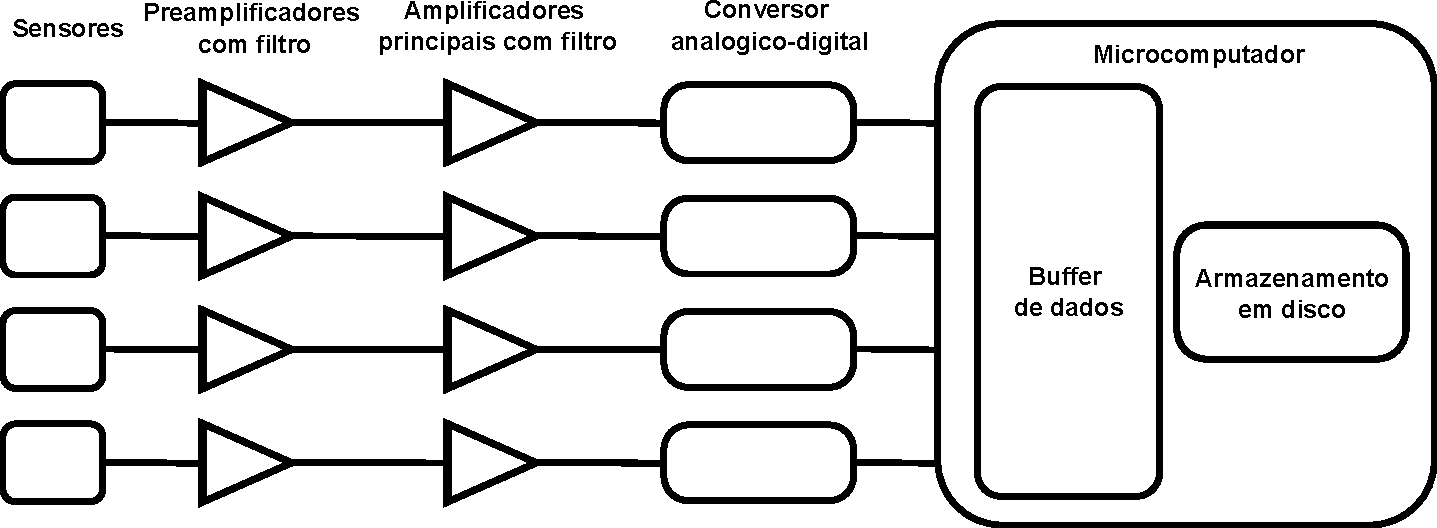
\includegraphics[width=.9\linewidth]{figs/Artigos/nde-ed-org/Figura1.pdf}
    \caption{Esquema funcional de um sistema de Emissão Acústica com sensores piezoelétricos, pré-amplificadores, filtros, amplificadores principais e sistema de aquisição digital. Adaptado de \citeonline{nde-ed-ae-equipment}.}
    \label{fig:nde-ed-org-Fig1}
\end{figure}

Inicialmente, os \textbf{sensores piezoelétricos} são fixados mecanicamente sobre a superfície do corpo de prova ou equipamento monitorado, utilizando acoplantes acústicos para otimizar a transmissão das ondas elásticas. Esses sensores são sensíveis a variações de pressão e deformações locais, produzindo um sinal elétrico \mbox{proporcional à amplitude da onda incidente}.

O sinal gerado pelo sensor é então encaminhado a um \textbf{pré-amplificador}, cuja função é elevar o nível de tensão do sinal original, geralmente na faixa de microvolts, para níveis adequados à posterior amplificação e filtragem. Em muitos sistemas, esse estágio inicial já incorpora filtros passa-faixa (tipicamente entre 100~kHz e 1~MHz), destinados a eliminar componentes de baixa frequência e ruídos ambientais, preservando apenas as frequências características dos eventos acústicos.

Em seguida, o sinal passa por um \textbf{amplificador principal}, também dotado de filtros ajustáveis, que permite o controle do ganho e a supressão de ruídos residuais. Essa dupla amplificação — pré e principal — é essencial para garantir uma relação sinal-ruído satisfatória, sobretudo em medições realizadas em ambientes industriais com \mbox{alta interferência eletromagnética.}

Após o condicionamento analógico, o sinal é direcionado a um \textbf{circuito de medição} que realiza a conversão analógico-digital, ADC, amostrando o sinal em altas taxas (geralmente entre 1~MHz e 40~MHz, dependendo da aplicação e do fenômeno estudado). Esses dados digitalizados são então armazenados temporariamente em um \textbf{\textit{buffer} de dados}, que atua como intermediário entre o \textit{front-end} analógico \mbox{e o sistema de processamento}.

O \textbf{microcomputador} ou unidade de controle central é responsável por gerenciar a aquisição e o armazenamento em disco, além de permitir o processamento dos sinais por meio de algoritmos dedicados à detecção de eventos, cálculo de parâmetros de emissão acústica (como amplitude, duração, energia e contagem de hits) e classificação de padrões. Em sistemas modernos, essa unidade também pode realizar a comunicação com interfaces externas, como APIs industriais, redes MODBUS ou sistemas supervisórios SCADA.

Por fim, o sistema é integrado a módulos de \textbf{visualização e controle}, permitindo que os resultados sejam exibidos em tempo real em um display ou monitor, e que o operador interaja por meio de um teclado ou interface gráfica. Essa visualização pode incluir formas de onda, histogramas de energia, espectros de frequência e alarmes automáticos quando limiares pré-definidos são excedidos.

Em conjunto, os elementos apresentados na Figura~\ref{fig:nde-ed-org-Fig1} compõem um sistema de aquisição e monitoramento de Emissão Acústica capaz de registrar, processar e analisar fenômenos transientes de alta frequência com elevada sensibilidade e precisão temporal. Esse tipo de arquitetura é amplamente empregado em pesquisas e aplicações industriais voltadas à detecção precoce de falhas estruturais, cavitação e fadiga de materiais, oferecendo uma alternativa não invasiva e altamente responsiva aos métodos tradicionais de inspeção.

Após a captação, o sinal adentra um circuito composto por \textbf{pré-amplificador}, \textbf{filtros} e \textbf{amplificador principal}, antes de ser \textbf{digitalizado} para análise computacional. Essa etapa é crucial porque eleva a relação sinal-ruído, atenua interferências eletromagnéticas e rejeita componentes espectrais alheios à banda de interesse; por essa razão, os pré-amplificadores costumam ser posicionados o mais próximo possível da fonte, reduzindo perdas por cabo e mitigando a suscetibilidade a ruídos acoplados.

A análise dos sinais de EA fornece dados cruciais por meio de parâmetros como \textbf{amplitude} (pico do sinal acima do nível de referência), \textbf{tempo de subida} (\textit{rise time}, usualmente do primeiro cruzamento de limiar ao pico), \textbf{duração} (intervalo durante o qual o sinal permanece acima do limiar), \textbf{contagens} (\textit{counts}, número de cruzamentos do limiar por um circuito comparador) e uma medida de \textbf{energia} associada ao evento. Na terminologia do \citeonline{nde-ed-ae-equipment}, essa energia é frequentemente chamada de \textbf{MARSE} (\textit{measured area under the rectified signal envelope}) e corresponde, de forma simplificada, à \textit{área sob o invólucro retificado} do sinal durante a janela do evento; detalhes são esquematizados na Figura~\ref{fig:nde-ed-org-Fig2}. Tais parâmetros não apenas permitem identificar e caracterizar “\textit{hits}” de emissão, mas também se prestam à separação entre ocorrências significativas e ruído de fundo, funcionando como indicadores robustos dos mecanismos físicos subjacentes ao dano.

\begin{figure}[H]
    \centering
    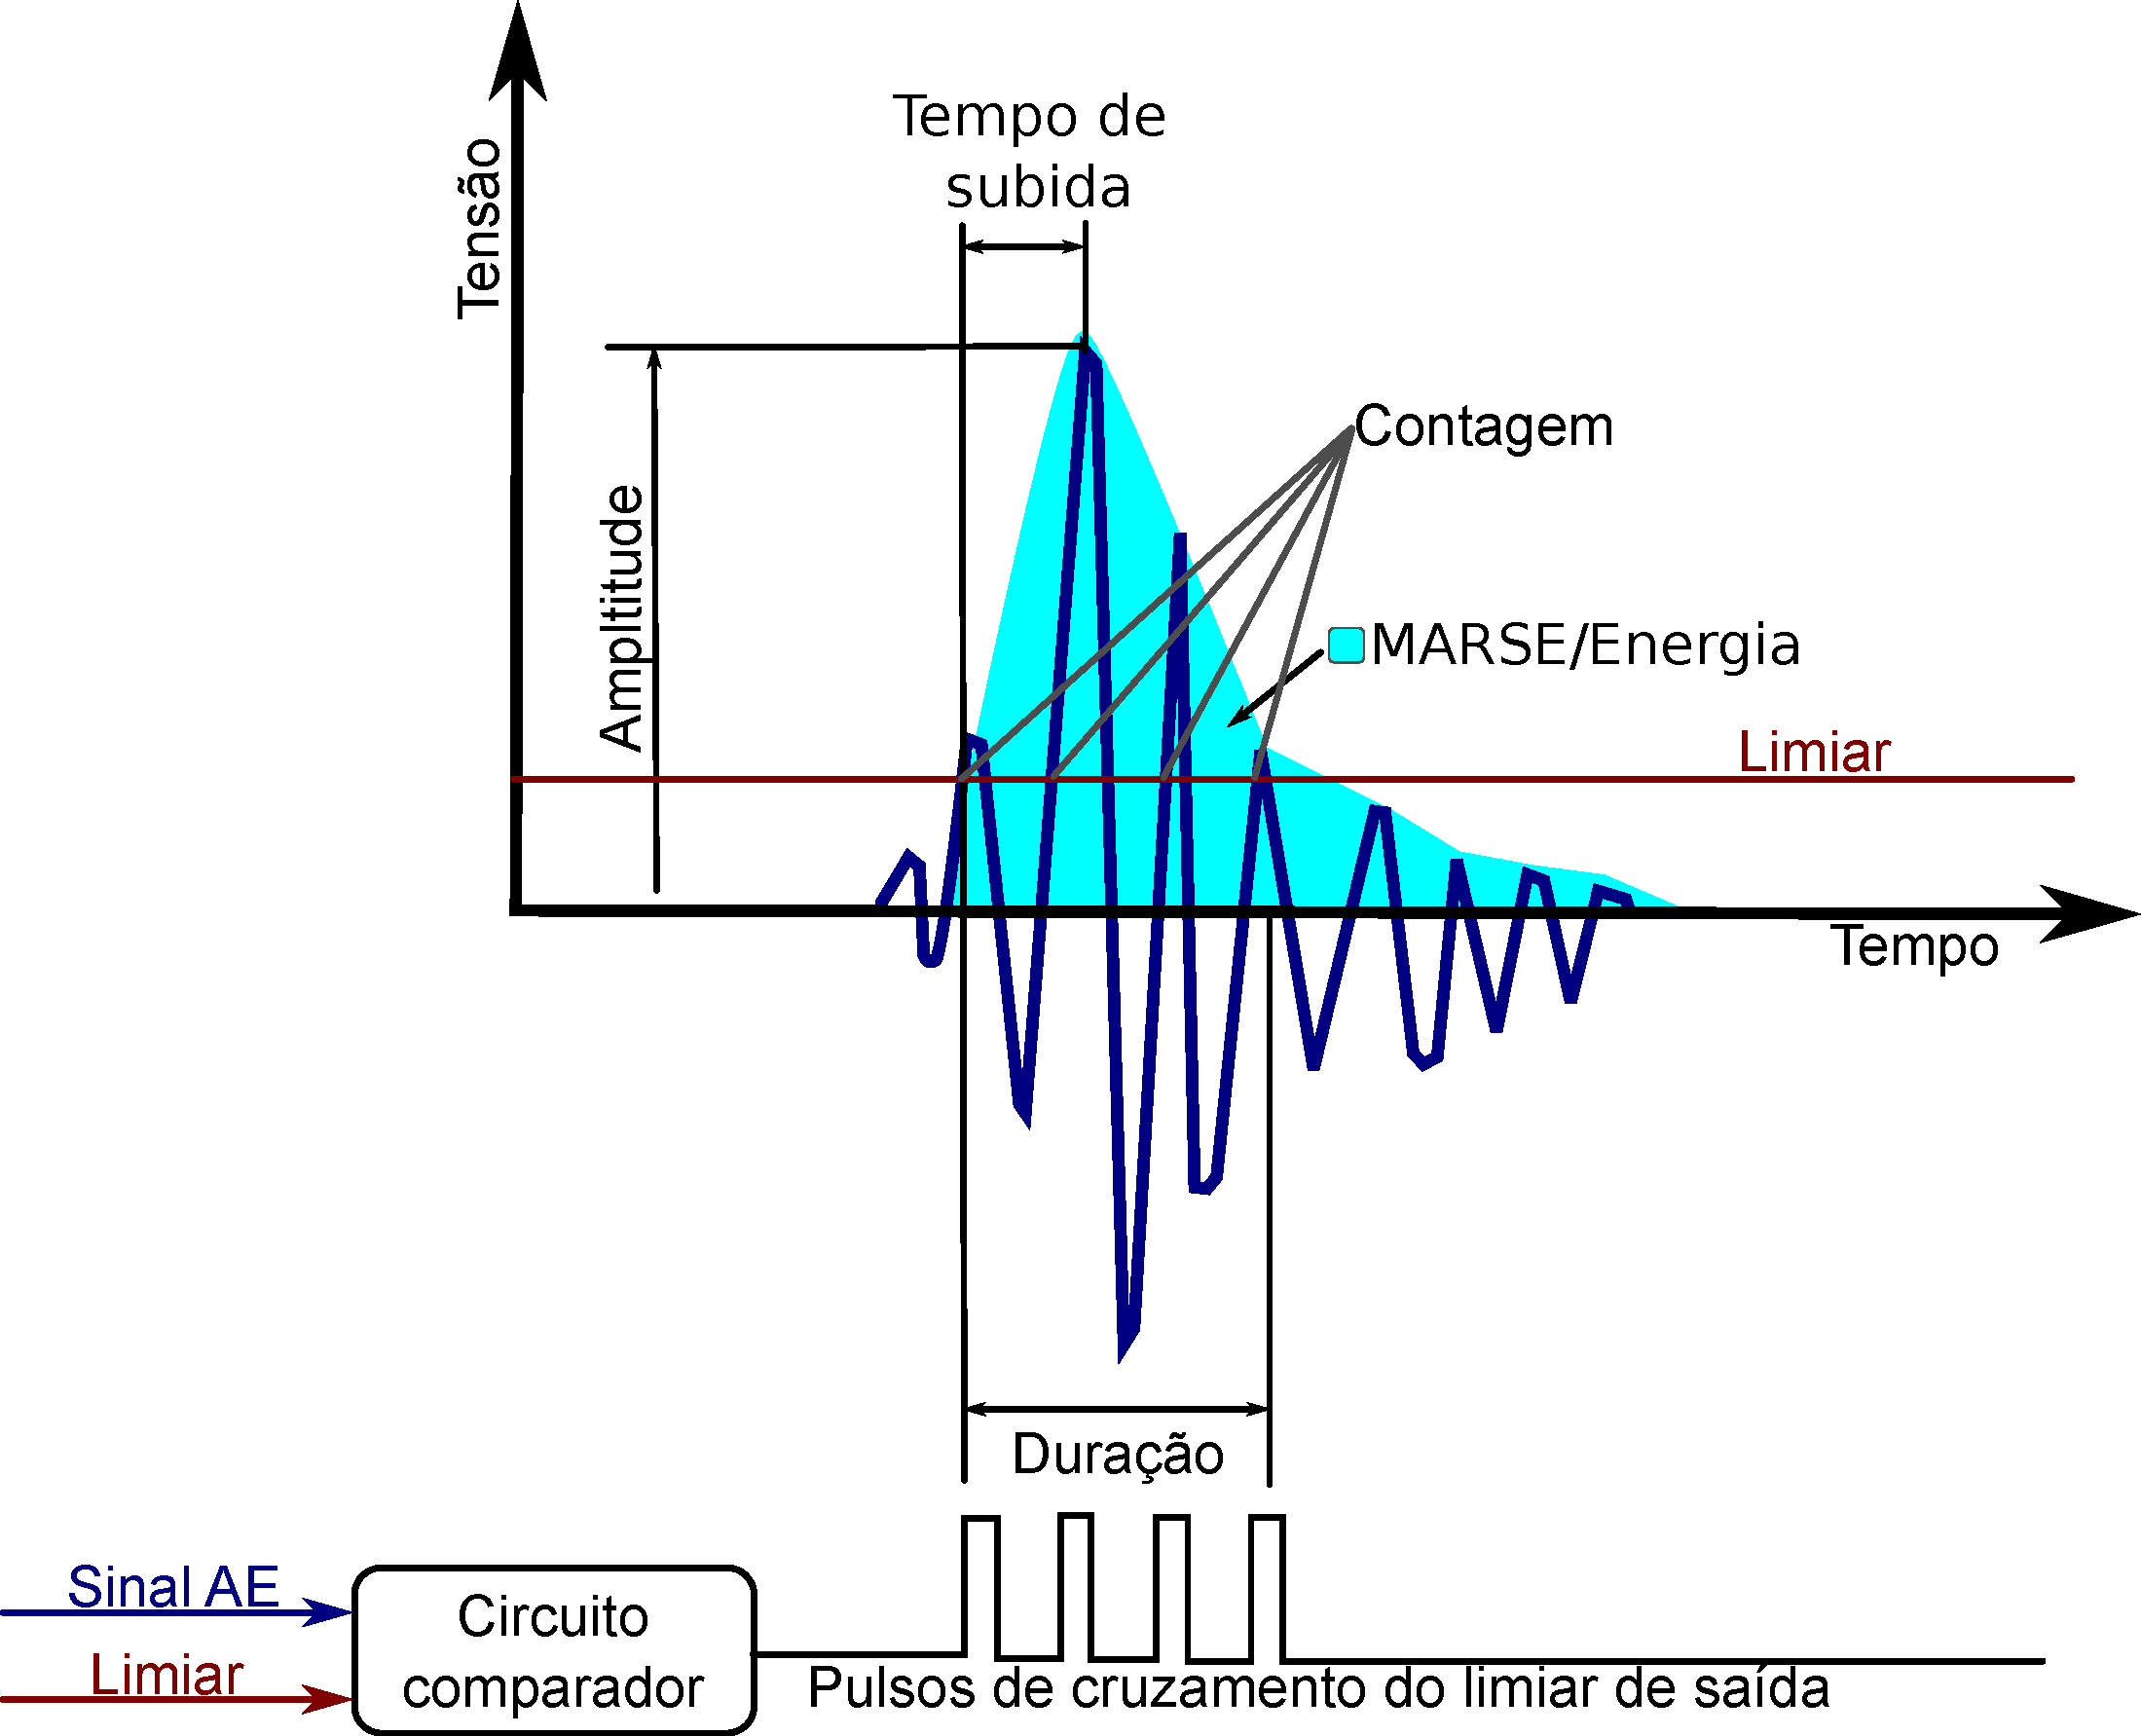
\includegraphics[width=.7\linewidth]{figs/Artigos/nde-ed-org/Figura2.pdf}
    \caption{Parâmetros clássicos extraídos de um “hit” de EA: amplitude, tempo de subida (\textit{rise time}), duração, contagens de limiar (\textit{counts}) e medida de energia (MARSE). O circuito comparador gera pulsos a cada cruzamento do limiar, contabilizados pelo sistema (adaptado de \citeonline{nde-ed-ae-equipment}).}
    \label{fig:nde-ed-org-Fig2}
\end{figure}

Do ponto de vista operacional, o \textbf{limiar} (\textit{threshold}) é definido sobre o nível de ruído para que a detecção seja seletiva. Um \textbf{hit} inicia no primeiro cruzamento desse limiar e se encerra quando o sinal permanece abaixo dele por um tempo de \textit{hit lockout} pré-definido. A partir daí, decompõem-se as grandezas:
\begin{itemize}
    \item \textbf{Amplitude} ($A_\text{pico}$): valor máximo do sinal acima do nível de referência dentro do hit.
    \item \textbf{Tempo de subida} ($t_\text{rise}$): intervalo do primeiro cruzamento de limiar até $A_\text{pico}$; é sensível à cinemática da fonte e à resposta do caminho de propagação.
    \item \textbf{Duração} ($t_\text{dur}$): tempo entre o primeiro e o último cruzamento do limiar; aumenta na presença de reverberações e múltiplas reflexões.
    \item \textbf{Contagens} (\textit{counts}): número de pulsos gerados pelo comparador a cada cruzamento de limiar; correlaciona-se com o conteúdo de alta frequência e a “granulosidade” do evento.
    \item \textbf{Energia (MARSE)}: área sob o invólucro retificado do sinal dentro da janela do hit.Matematicamente, a forma \textit{MARSE} pode ser escrita, em uma discretização simples,~como apresentada em \ref{eq:marse}. 
    
    \begin{equation}
    	\label{eq:marse}
    	\text{MARSE} \;\approx\; \sum_{n=n_0}^{n_1} \big|\,x[n]\,\big| \;\Delta t
    	\quad\text{ou}\quad
    	\text{MARSE} \;\approx\; \sum_{n=n_0}^{n_1} e[n] \;\Delta t,
    \end{equation}
    %$$
    %\text{MARSE} \;\approx\; \sum_{n=n_0}^{n_1} \big|\,x[n]\,\big| \;\Delta t
    %\quad\text{ou}\quad
    %\text{MARSE} \;\approx\; \sum_{n=n_0}^{n_1} e[n] \;\Delta t,
    %$$
    
    em que $x[n]$ é o sinal de EA amostrado e $e[n]$ denota o invólucro (por exemplo, obtido por retificação + filtragem passa-baixas, ou por transformada de Hilbert). Essa métrica captura \textit{quanta de atividade} ao longo do hit, sendo bastante utilizada por fornecedores de instrumentação de EA e por materiais de referência \mbox{educacionais como o \citeonline{nde-ed-ae-equipment}.}
\end{itemize}

\noindent\textbf{{Observação sobre nomenclatura de energia.}}

É importante salientar que \textbf{não há consenso terminológico} na literatura quanto à ``energia'' do evento de EA. Enquanto o \citeonline{nde-ed-ae-equipment} emprega \textit{MARSE} (área do invólucro retificado), revisões de estado da arte, como \citeonline{liu2023review}, frequentemente utilizam \textbf{energia baseada em potência instantânea}, aproximada pela soma dos quadrados da amplitude (proporcional a energia acústica sob hipóteses de linearidade do caminho e calibração adequada, \mbox{como apresentada em \ref{eq:energia}:}

\begin{equation}
	\label{eq:energia}
	E_\text{sq} \;\propto\; \sum_{n=n_0}^{n_1} x^2[n] \;\Delta t.
\end{equation}

Em aplicações comparativas,por exemplo, na distinção entre cavitação incipiente e regimes estabelecidos,essa diferença \textit{conceitual} pode impactar limiares de decisão, escalas de normalização e correlações com grandezas físicas. Por isso, ao longo desta dissertação, quando nos referirmos a \textbf{MARSE}, estaremos explicitamente adotando a \textit{área do invólucro retificado}; quando nos referirmos à \textbf{energia quadrática} (ou simplesmente “energia” na acepção de \citeonline{liu2023review}), estaremos empregando a soma dos quadrados da amplitude. Sempre que pertinente, serão fornecidas ambas as métricas, devidamente normalizadas, de modo a preservar a comparabilidade com diferentes fontes bibliográficas e práticas~de~instrumentação.


O diferencial da técnica reside em seu caráter passivo — ela ``ouve'' a emissão real do material sob carga, ao invés de estimular o componente, como ocorre em métodos como ultrassom ou radiografia. Isso permite monitoramento contínuo e não intrusivo em condições operacionais reais, captando apenas fontes ativas de dano e cobrindo grandes volumes estruturais com um número reduzido de sensores.

Além disso, sistemas de EA podem operar com localização acústica da fonte emissora, utilizando redes de sensores e analisando as diferenças de tempo de chegada do sinal (métodos linear, planar ou volumétrico), o que permite determinar a posição exata de emissão dentro da estrutura.

Esses parâmetros, além de fornecerem informações físicas sobre a natureza do evento, constituem também a base para a extração de \textit{features} no contexto de aprendizado de máquina. Em abordagens modernas de análise de sinais de Emissão Acústica, como a proposta neste trabalho, o conjunto de atributos derivados desses parâmetros — tanto no domínio do tempo quanto no domínio da frequência — é utilizado para representar cada evento (\textit{hit}) de forma compacta e informativa, facilitando sua posterior~classificação~por~redes neurais.

No domínio do tempo, são extraídos descritores diretos, como amplitude, duração, tempo de subida, energia (MARSE ou energia quadrática), número de contagens e razão entre parâmetros (por exemplo, a razão entre energia e duração, indicativa da intensidade relativa do evento). Já no domínio da frequência, técnicas de análise espectral, como a Transformada Rápida de Fourier (FFT) ou a Transformada de Short-Time Fourier (STFT), permitem a identificação de componentes dominantes e a distinção entre regimes acústicos característicos — como cavitação incipiente, cavitação plena e ruído mecânico.

Durante o pré-processamento, esses parâmetros são normalizados com base em janelas móveis e limiares de ruído, garantindo que variações instrumentais ou ambientais não influenciem indevidamente o processo de aprendizagem. As janelas de tempo são segmentadas e rotuladas conforme as classes de operação (\textit{normal}, \textit{cavitação} ou \textit{falha estrutural}), e o conjunto de sinais normalizados é então utilizado como \mbox{entrada para o treinamento da CNN-1D.}

Nesse contexto, a rede convolucional atua como uma extensão automática do processo de extração de \textit{features}, aprendendo representações hierárquicas diretamente das formas de onda ou dos espectrogramas derivados. Essa combinação entre parâmetros clássicos da Emissão Acústica e aprendizado profundo forma uma abordagem híbrida que alia a interpretabilidade dos métodos tradicionais à robustez e adaptabilidade dos modelos modernos de Inteligência Artificial, conforme ilustrado no fluxograma geral dos objetivos~da pesquisa (Figura~\ref{fig:fluxograma_geral}).

Ademais, a onda primitiva originada em um evento de EA é tipicamente de curta duração (microssegundos) e pode apresentar forte direcionalidade e variabilidade na amplitude, dependendo da natureza física da falha, como deformação cristalina ou fraturas progressivas. Sua propagação é influenciada por fatores como atenuações geométricas, estruturais e pela dispersão devido à microestrutura do material, \mbox{como os contornos de grão e inclusões.}

É importante ressaltar que nem toda emissão EA indica falha estrutural: fenômenos como fricção mecânica, vazamentos e pulsos por cavitação ou descargas parciais podem produzir sinais semelhantes aos genuínos, classificados como pseudo-fontes. A aplicação de filtros avançados, avaliação espectral e critérios baseados em tempo de chegada são estratégias fundamentais para distinguir esses eventos e minimizar falsos positivos.

Em síntese, a técnica de Emissão Acústica apresenta-se como uma abordagem promissora para o monitoramento em tempo real e a detecção precoce de falhas estruturais, devido à sua alta sensibilidade e natureza não intrusiva. A compreensão de seus princípios físicos e dos parâmetros característicos extraídos dos sinais é essencial para a correta interpretação dos fenômenos observados, como trincas, desgaste superficial e cavitação em bombas centrífugas. A seguir, são discutidos estudos representativos que exploram a aplicação da Emissão Acústica em sistemas hidráulicos e turbomáquinas, evidenciando as metodologias empregadas, os resultados obtidos e as limitações que \mbox{motivam o presente~trabalho.}

\subsection{Revisão de Pesquisas sobre Emissão Acústica}

Segundo \citeonline{liu2023review}, a cavitação em bombas é um fenômeno multifásico inevitável que provoca a formação e colapso de bolhas quando a pressão local do escoamento cai abaixo da pressão de vapor do líquido. Esse processo resulta em perda de desempenho hidráulico, erosão de componentes, vibração excessiva e ruído característico, podendo até gerar falhas estruturais. A detecção precoce, portanto, tem grande relevância tanto para a segurança operacional quanto para a redução de custos de manutenção.

Os autores revisam diferentes metodologias de detecção baseadas em sinais, como vibração, emissão acústica, ruído hidrodinâmico e pulsação de pressão. Conforme ilustrado no fluxograma da Figura~\ref{fig:LiuFig1}, tais métodos seguem um fluxo comum: aquisição de sinais em pontos estratégicos da bomba, processamento nos domínios do tempo, frequência ou tempo–frequência, extração de parâmetros característicos e, por fim, identificação do estado de cavitação com auxílio de algoritmos de inteligência artificial. A Figura~\ref{fig:LiuFig2} resume essas metodologias de pesquisa.

\begin{figure}[H]
    \centering
    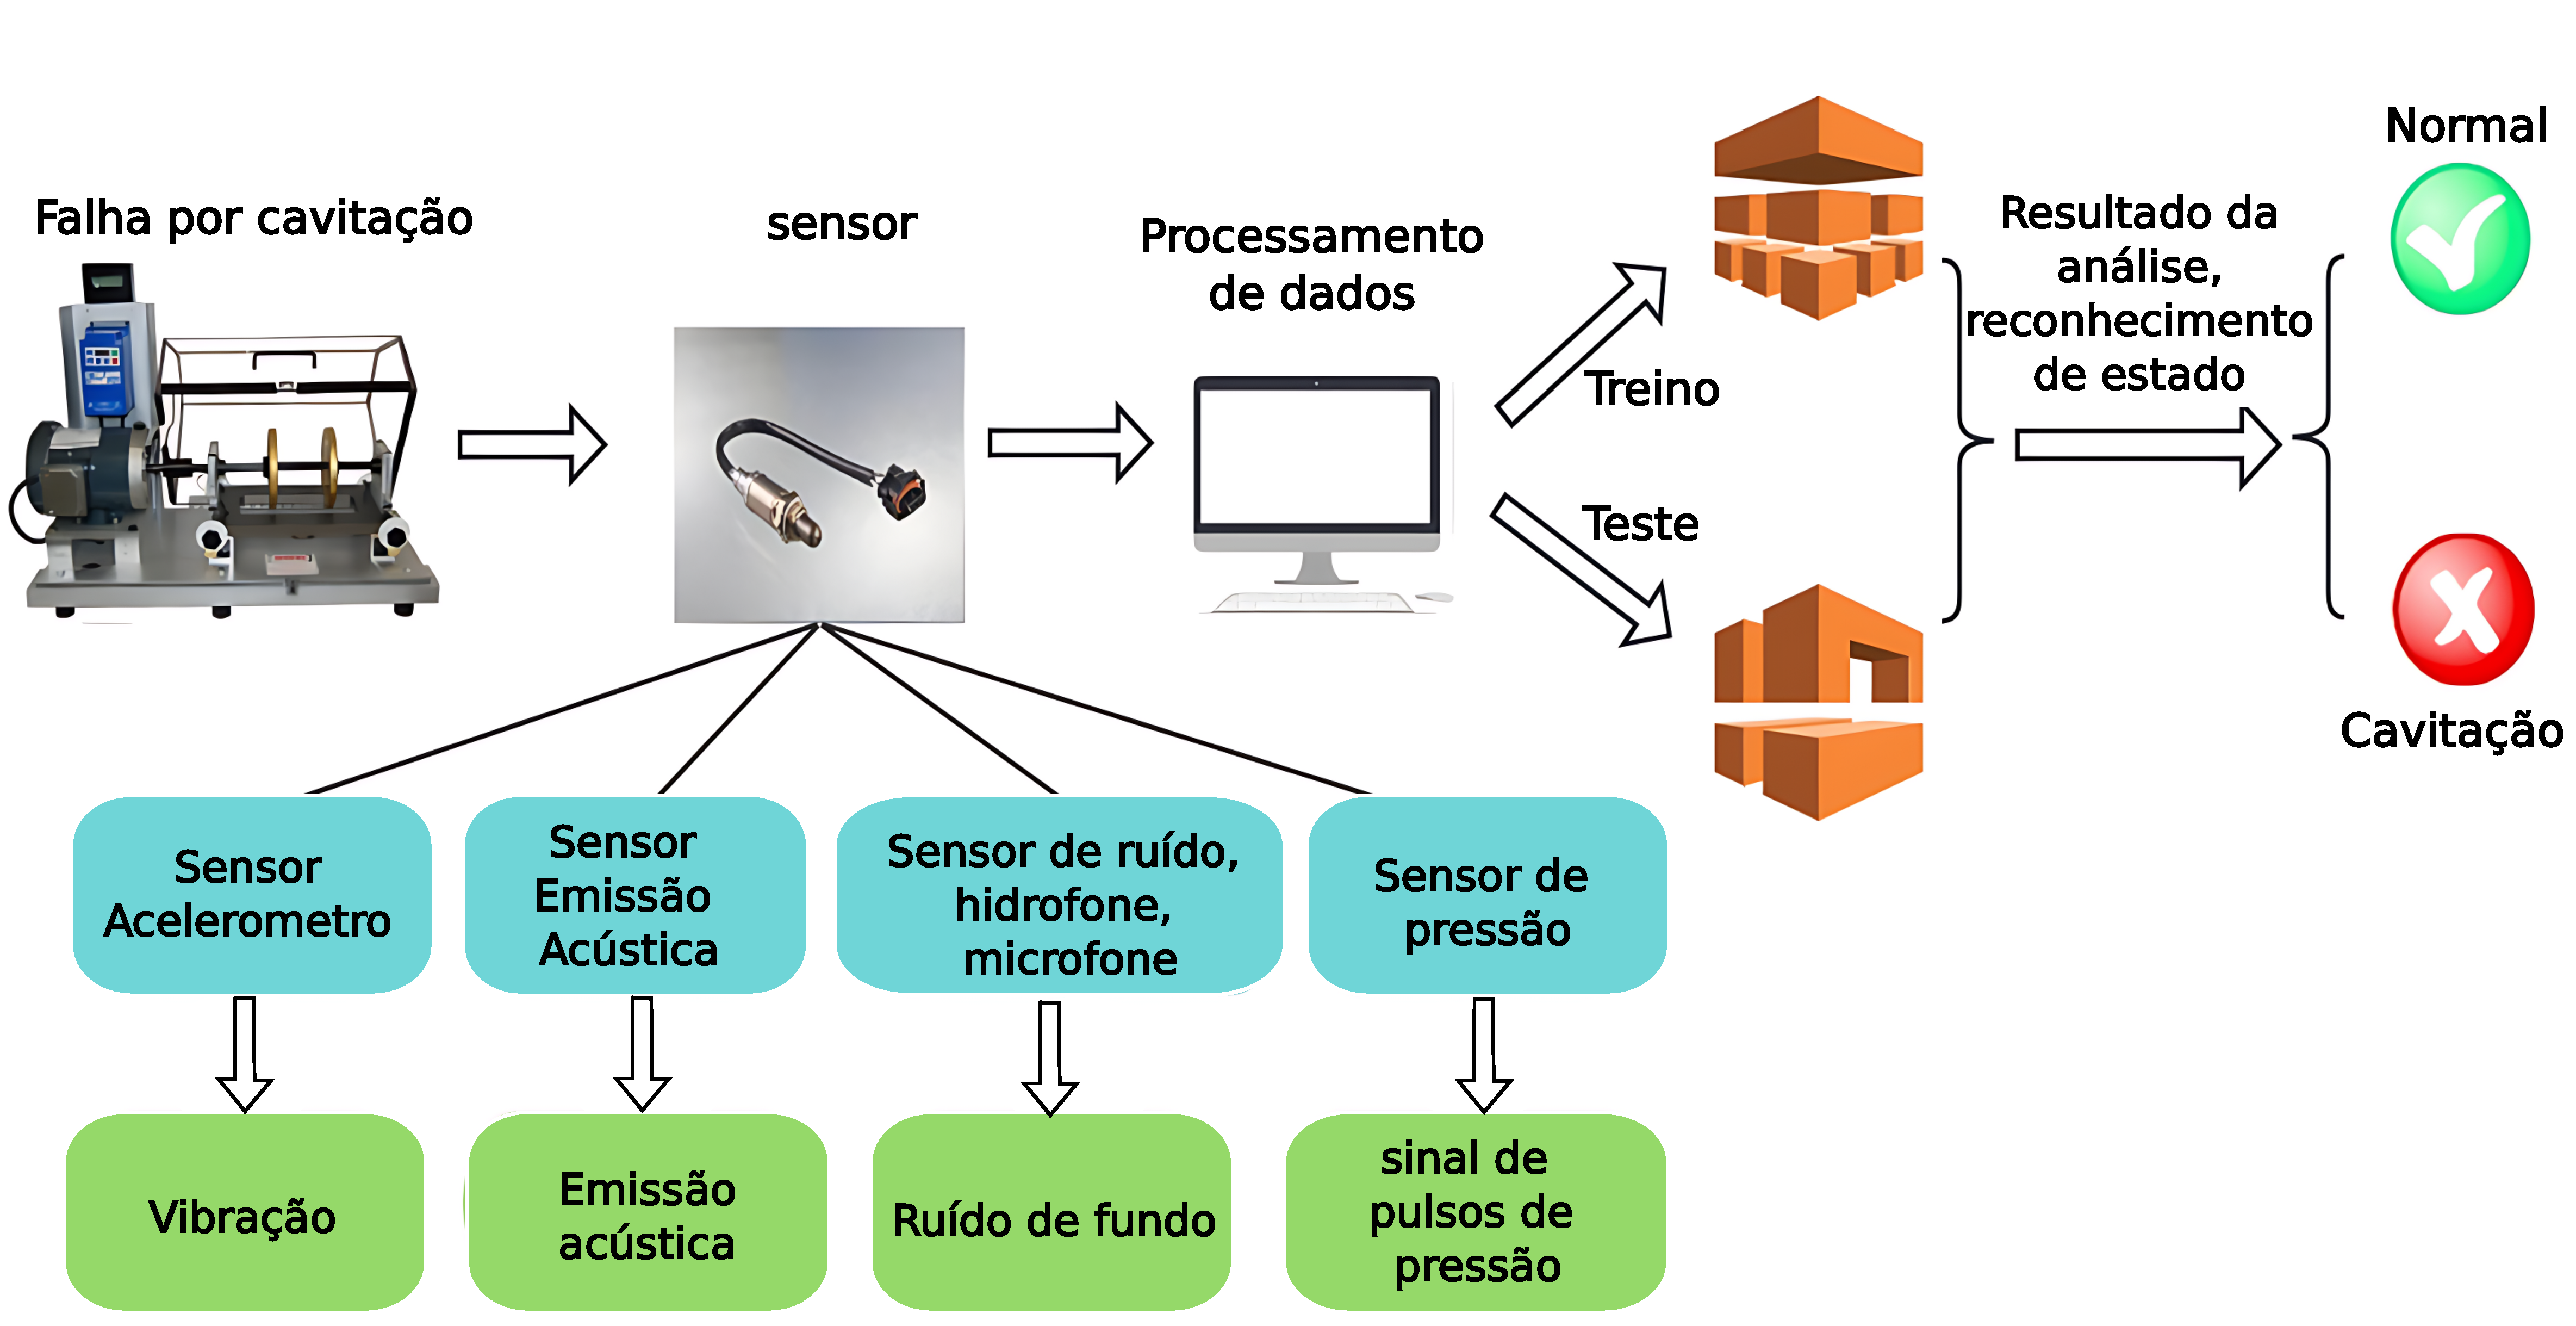
\includegraphics[width=1\linewidth]{figs/Artigos/Liu/Figura1.pdf}
    \caption{Fluxograma básico de detecção de cavitação com base em diferentes sinais. Adaptado de \citeonline{liu2023review}.}
    \label{fig:LiuFig1}
\end{figure}

O diagrama da Figura~\ref{fig:LiuFig1} organiza a detecção por \textbf{famílias de sinais} e explicita a relação entre a física da cavitação e o canal sensorial:
\begin{itemize}
    \item \textbf{Sinal de vibração (acelerômetros):} sensível à excitação mecânica do conjunto rotor–estator; captura impactos e modulações de banda larga provocadas pelo colapso de bolhas e por fenômenos associados, entre outros efeitos (desbalanceamento secundário, instabilidades hidráulicas).
    
    \item \textbf{Sinal de emissão acústica (sensores piezoelétricos):} focaliza faixas de alta frequência (tipicamente centenas de kHz), nas quais eventos transientes de cavitação apresentam razão sinal–ruído elevada; adequado à detecção incipiente.
    \item \textbf{Sinal de ruído (microfones/hidrofones):} capta componentes aéreas ou no fluido; informativo para estágios mais intensos de cavitação e para varreduras rápidas, embora mais suscetível a interferências ambientais.
    \item \textbf{Pulsação de pressão (transdutores de pressão):} evidencia flutuações periódicas/quasi-periódicas do campo de pressão; útil para mapear regimes e instabilidades do escoamento.
\end{itemize}
A linha intermediária do diagrama explicita que \textbf{cada sensor observa um aspecto da cavitação}: os sinais carregam assinaturas distintas (impactos, bandas espectrais, intermitência, modulações). A partir daí, o fluxo converge para \textbf{processamento de sinais} (métricas no tempo: RMS, pico, curtose, crest factor; no espectro: centroides, bandas energéticas; no tempo–frequência: STFT, wavelets), seguido de \textbf{extração de atributos} e \textbf{reconhecimento de estado} por algoritmos de IA (por exemplo, \textit{SVM}, \textit{Random Forest}, \textit{k-NN}, e redes profundas como CNN-1D/2D ou \textit{LSTM}). Em síntese, a figura mostra que, embora os canais sensoriais sejam diversos, o \textit{pipeline lógico} é comum e modular.

\begin{figure}[H]
    \centering
    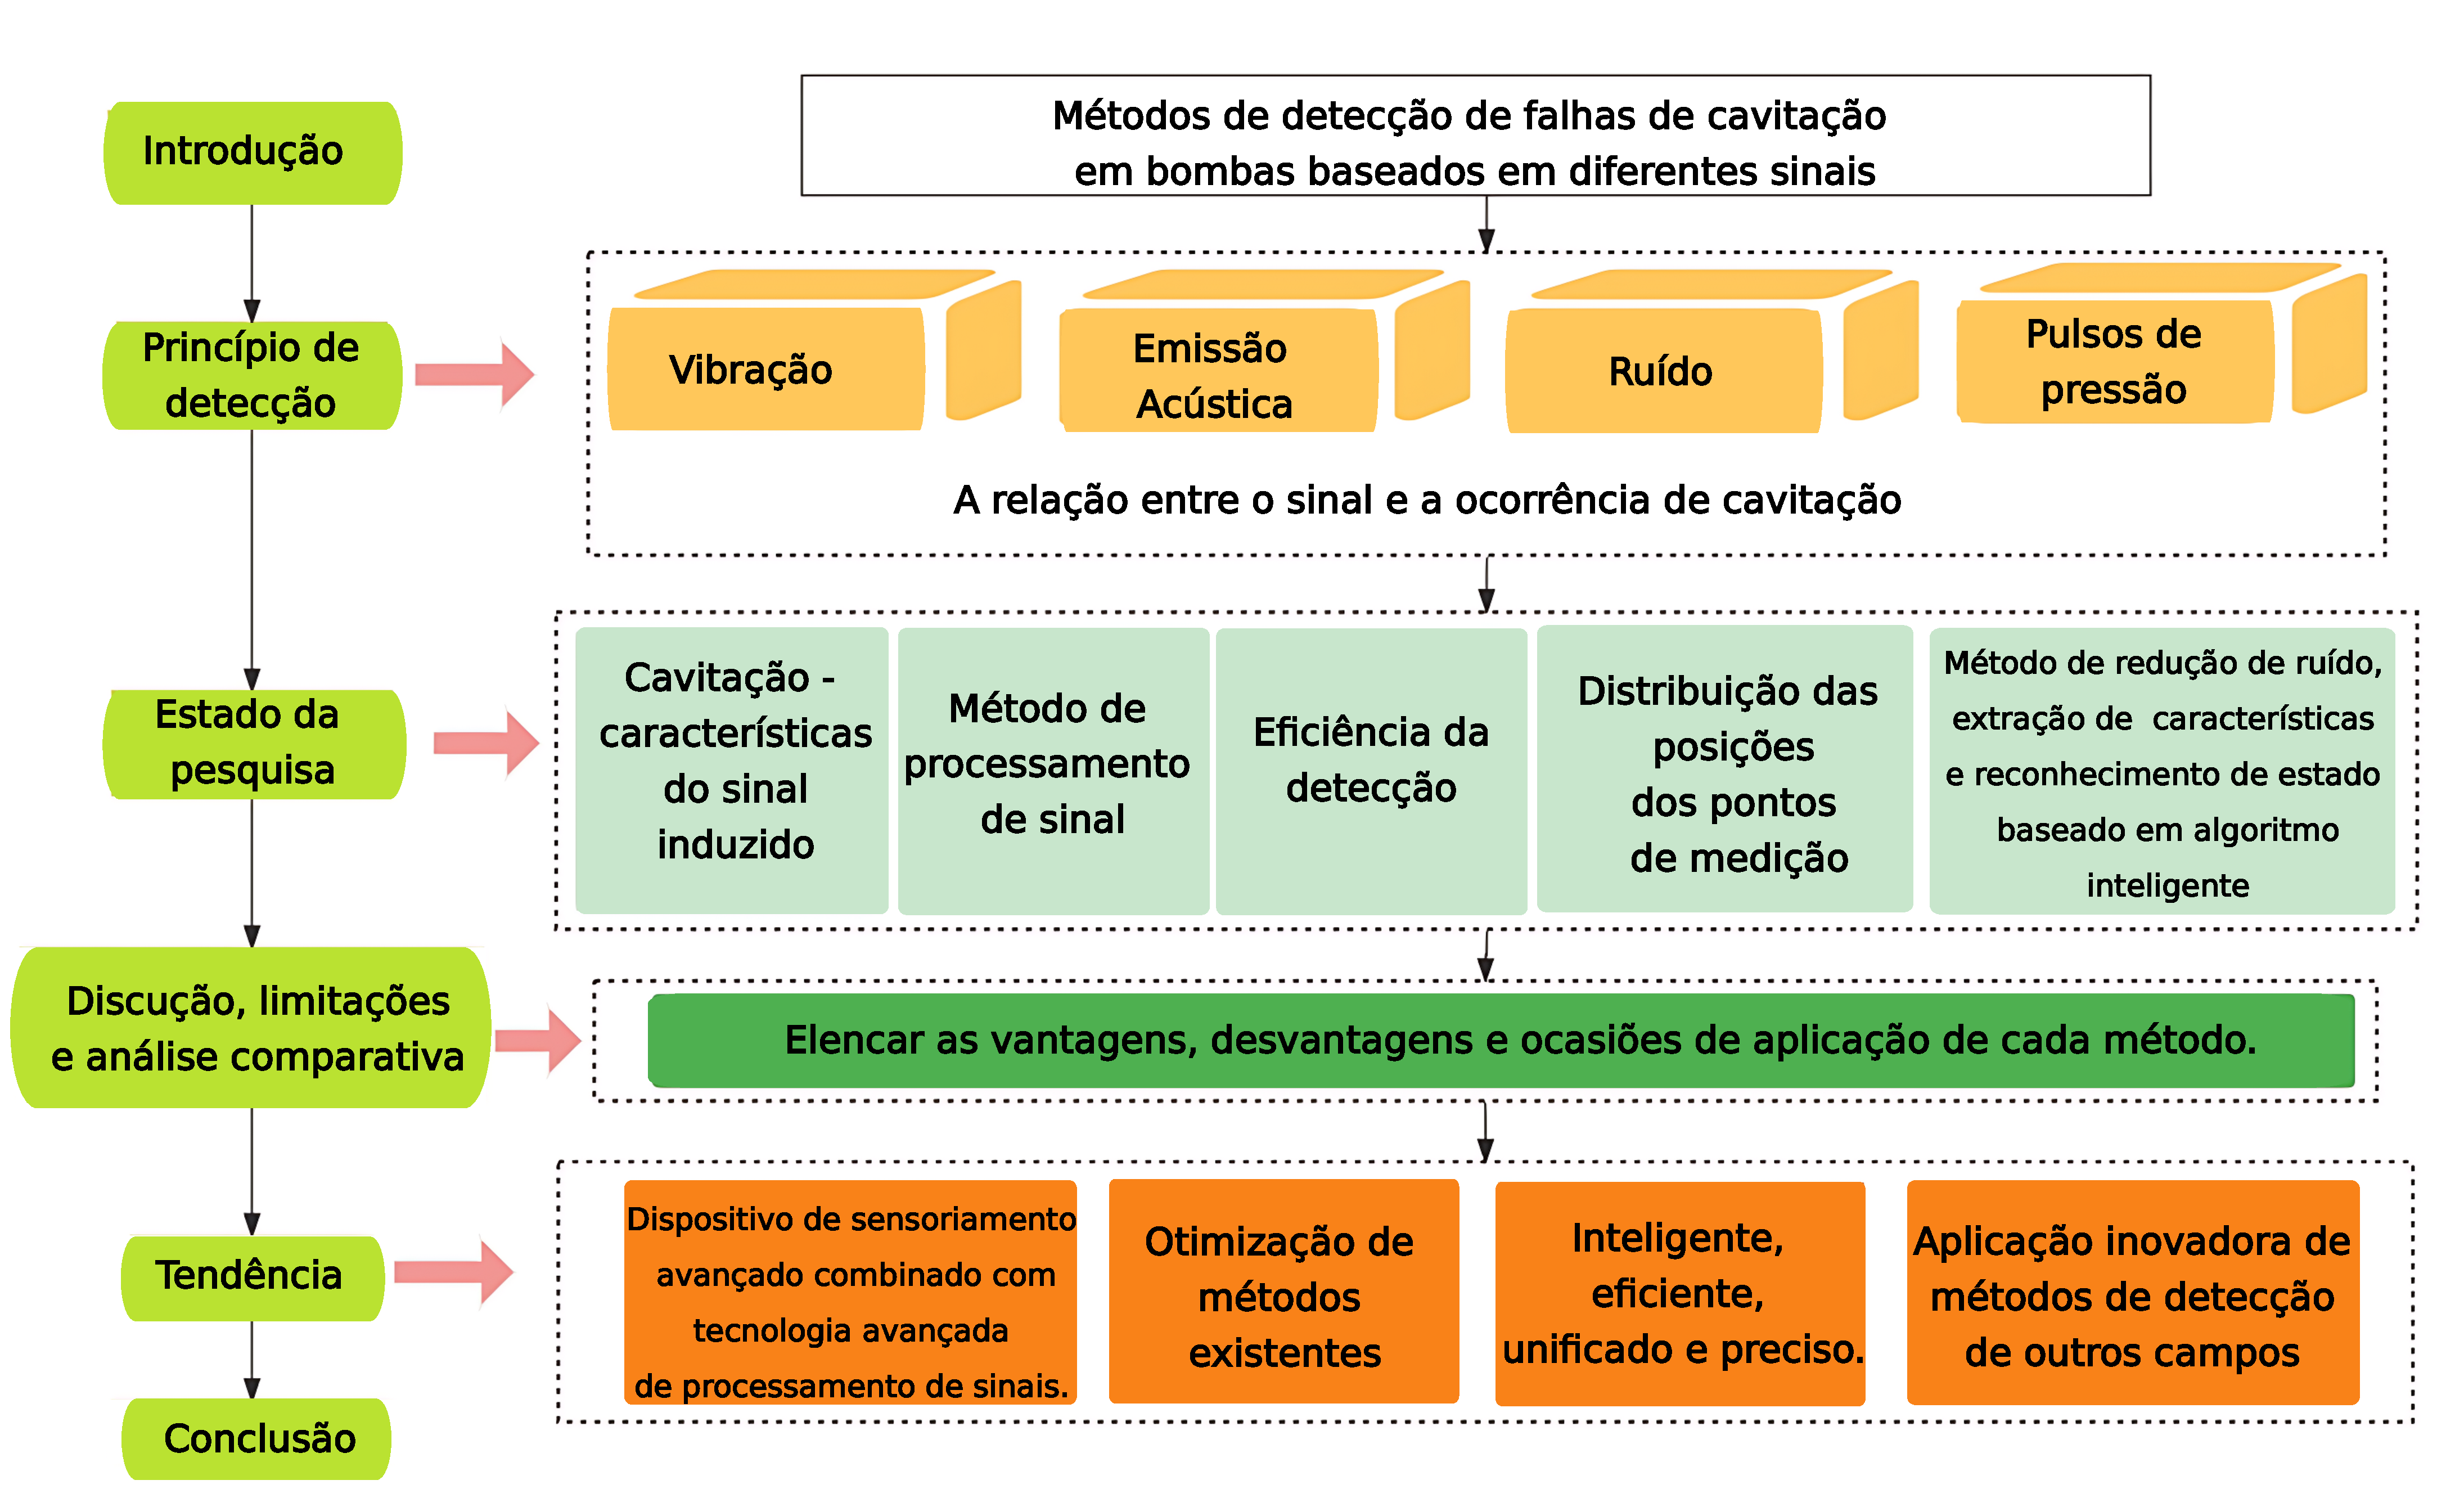
\includegraphics[width=1\linewidth]{figs/Artigos/Liu/Figura2.pdf}
    \caption{Diagrama principal do conteúdo da pesquisa do artigo. Adaptado de \citeonline{liu2023review}. }
    \label{fig:LiuFig2}
\end{figure}

Com o objetivo de mapear os desafios do monitoramento de condição, o esquema ilustrado na Figura~\ref{fig:LiuFig2} sintetiza o \textbf{ciclo de pesquisa} em cinco camadas essenciais. Tal segmentação abrange desde a caracterização do problema de desempenho e integridade em bombas até a implementação de soluções inteligentes unificadas, compreendendo os seguintes tópicos:

\linespread{1.27}\selectfont
\begin{enumerate}
    \item \textbf{Introdução:} contextualiza a cavitação como problema de desempenho e integridade; define objetivos (detecção incipiente, redução de custos, aumento de confiabilidade).
    \item \textbf{Princípio de detecção:} relaciona a \textit{origem física} da cavitação com o \textit{que cada sensor enxerga}. Por exemplo, o colapso de bolhas gera altas frequências (AE), enquanto flutuações de pressão se refletem mais nos transdutores de pressão e na vibração de baixa/média frequência.
    \item \textbf{Estado da pesquisa:} quatro eixos críticos:
    \begin{enumerate}[label=\alph*)]
        \item \textit{Características induzidas pela cavitação:} intermitência, assimetria estatística, picos espectrais e alargamento de banda; mudanças em curtose, entropias e taxas de cruzamento por limiar.
        \item \textit{Métodos de processamento de sinais:} do básico (filtros, estatísticas de ordem superior) ao avançado (STFT, CWT, espectrogramas, \textit{scalograms}, cepstra).
        \item \textit{Eficiência de detecção:} métricas (acurácia, sensibilidade, especificidade, AUC, F1), além de latência e robustez a ruído; aqui entram comparações sistemáticas entre algoritmos e sensores.
        \item \textit{Posicionamento de pontos de medição:} trade-offs entre proximidade do fenômeno, acessibilidade, segurança, custo e suscetibilidade a ruído estrutural/ambiental.
    \end{enumerate}
    \item \textbf{Discussão, limitações e comparação:} consolida \textit{vantagens e desvantagens} de cada canal/sensor: AE destaca-se na detecção incipiente e em altas frequências, vibração é amplamente disponível e barata, pressão é direta para regimes hidráulicos, ruído é fácil de instrumentar porém sensível a ambiente. Também discute limitações (calibração, variabilidade do escoamento, repetibilidade, datasets pequenos).
    \item \textbf{Tendências:} quatro direções estratégicas:
    \begin{enumerate}[label=\alph*)]
        \item \textit{Sensoriamento avançado + processamento avançado:} sensores banda-larga, arrays, sincronização multicanal; pipelines tempo–frequência e fusão multimodal.
        \item \textit{Otimização de métodos existentes:} melhor seleção de \textit{features}, redução de dimensionalidade, aprendizado semi-supervisionado e \textit{few-shot}.
        \item \textit{Sistemas inteligentes, unificados e acurados:} do laboratório ao campo, com atenção à \textbf{latência}, \textbf{robustez a ruído} e \textbf{generalização} entre bombas/condições.
        \item \textit{Transferência de métodos de outras áreas:} técnicas maduras de diagnóstico de máquinas, sonar/ultrassom e visão computacional (ex., CNNs 1D/2D, transformers específicos para séries temporais).
    \end{enumerate}
\end{enumerate}


Em síntese, as Figuras \ref{fig:LiuFig1} e \ref{fig:LiuFig2} evidenciam que a detecção de cavitação tem evoluído de abordagens puramente empíricas para arquiteturas \textbf{modulares e orientadas a dados}, nas quais a escolha do sensor, a estratégia de processamento e o modelo de classificação integram-se em um \textit{pipeline} unificado e flexível. Essa estrutura permite adaptar metodologias de diagnóstico a distintos contextos industriais, conciliando precisão, \mbox{tempo de resposta e viabilidade de implementação.}

Sob essa perspectiva, os estudos analisados reforçam a motivação central desta pesquisa: investigar a cadeia de processamento que envolve o \textbf{pré-processamento}, a \textbf{extração e representação de atributos} e a \textbf{classificação por meio de uma CNN-1D}, com o objetivo de alcançar uma detecção de cavitação rápida, robusta e energeticamente eficiente. Ao mesmo tempo, mantém-se a perspectiva de integração futura dessas técnicas em \textit{hardware} reconfigurável, consolidando um caminho viável para soluções embarcadas de monitoramento inteligente.


Entre os diversos métodos analisados por \citeonline{liu2023review}, o monitoramento por vibração se destaca como o mais consolidado e amplamente aplicado em sistemas hidráulicos industriais. Alterações expressivas na resposta espectral, especialmente o surgimento de picos em faixas de 2 kHz a 8 kHz, constituem indicadores diretos da presença de cavitação — fenômeno ilustrado nas Figuras \ref{fig:LiuFig4A} e \ref{fig:LiuFig4B}. A primeira demonstra a diferença temporal entre regimes de operação com e sem cavitação, evidenciando o aumento abrupto da amplitude e da irregularidade do sinal. Já a segunda mostra, no domínio da frequência, o deslocamento da energia espectral e a intensificação de componentes harmônicas conforme a rotação da bomba aumenta, comportamento que reflete a instabilidade hidrodinâmica \mbox{provocada pelo colapso das bolhas.}

Apesar de sua maturidade tecnológica, o método de vibração apresenta sensibilidade limitada à cavitação incipiente, uma vez que os sinais gerados nos estágios iniciais do fenômeno são de baixa amplitude e facilmente mascarados por ruídos mecânicos ou estruturais. Nesse contexto, a técnica de \textbf{Emissão Acústica, EA} desponta como alternativa mais sensível e informativa. Essa abordagem capta as ondas elásticas transitórias geradas por microjatos e choques associados ao colapso de cavidades, abrangendo uma faixa espectral que se estende de aproximadamente 1 kHz a 1 MHz.

Os parâmetros derivados do sinal, como \textbf{amplitude}, \textbf{duração}, \textbf{energia} e \textbf{contagens acima do limiar} (ou “counts”), mostrados na Figura \ref{fig:LiuFig6}, constituem indicadores diretos da intensidade e da frequência de ocorrência dos eventos acústicos. Esses parâmetros — amplamente empregados em sistemas de monitoramento baseados em hits — permitem não apenas detectar a cavitação incipiente, mas também avaliar a severidade do processo de erosão associada. No entanto, sua adoção em ambientes industriais ainda é desafiada por fatores como o custo dos sensores piezoelétricos de alta sensibilidade, a necessidade de acoplamento preciso e a suscetibilidade à interferência estrutural.

Assim, enquanto os sensores de vibração oferecem uma visão global e robusta do comportamento dinâmico do conjunto rotativo, a emissão acústica fornece uma janela privilegiada para o diagnóstico precoce, sendo particularmente promissora para integração futura com plataformas embarcadas de detecção inteligente — foco desta pesquisa.
\linespread{1.25}\selectfont

\begin{figure}[H]
    \centering
    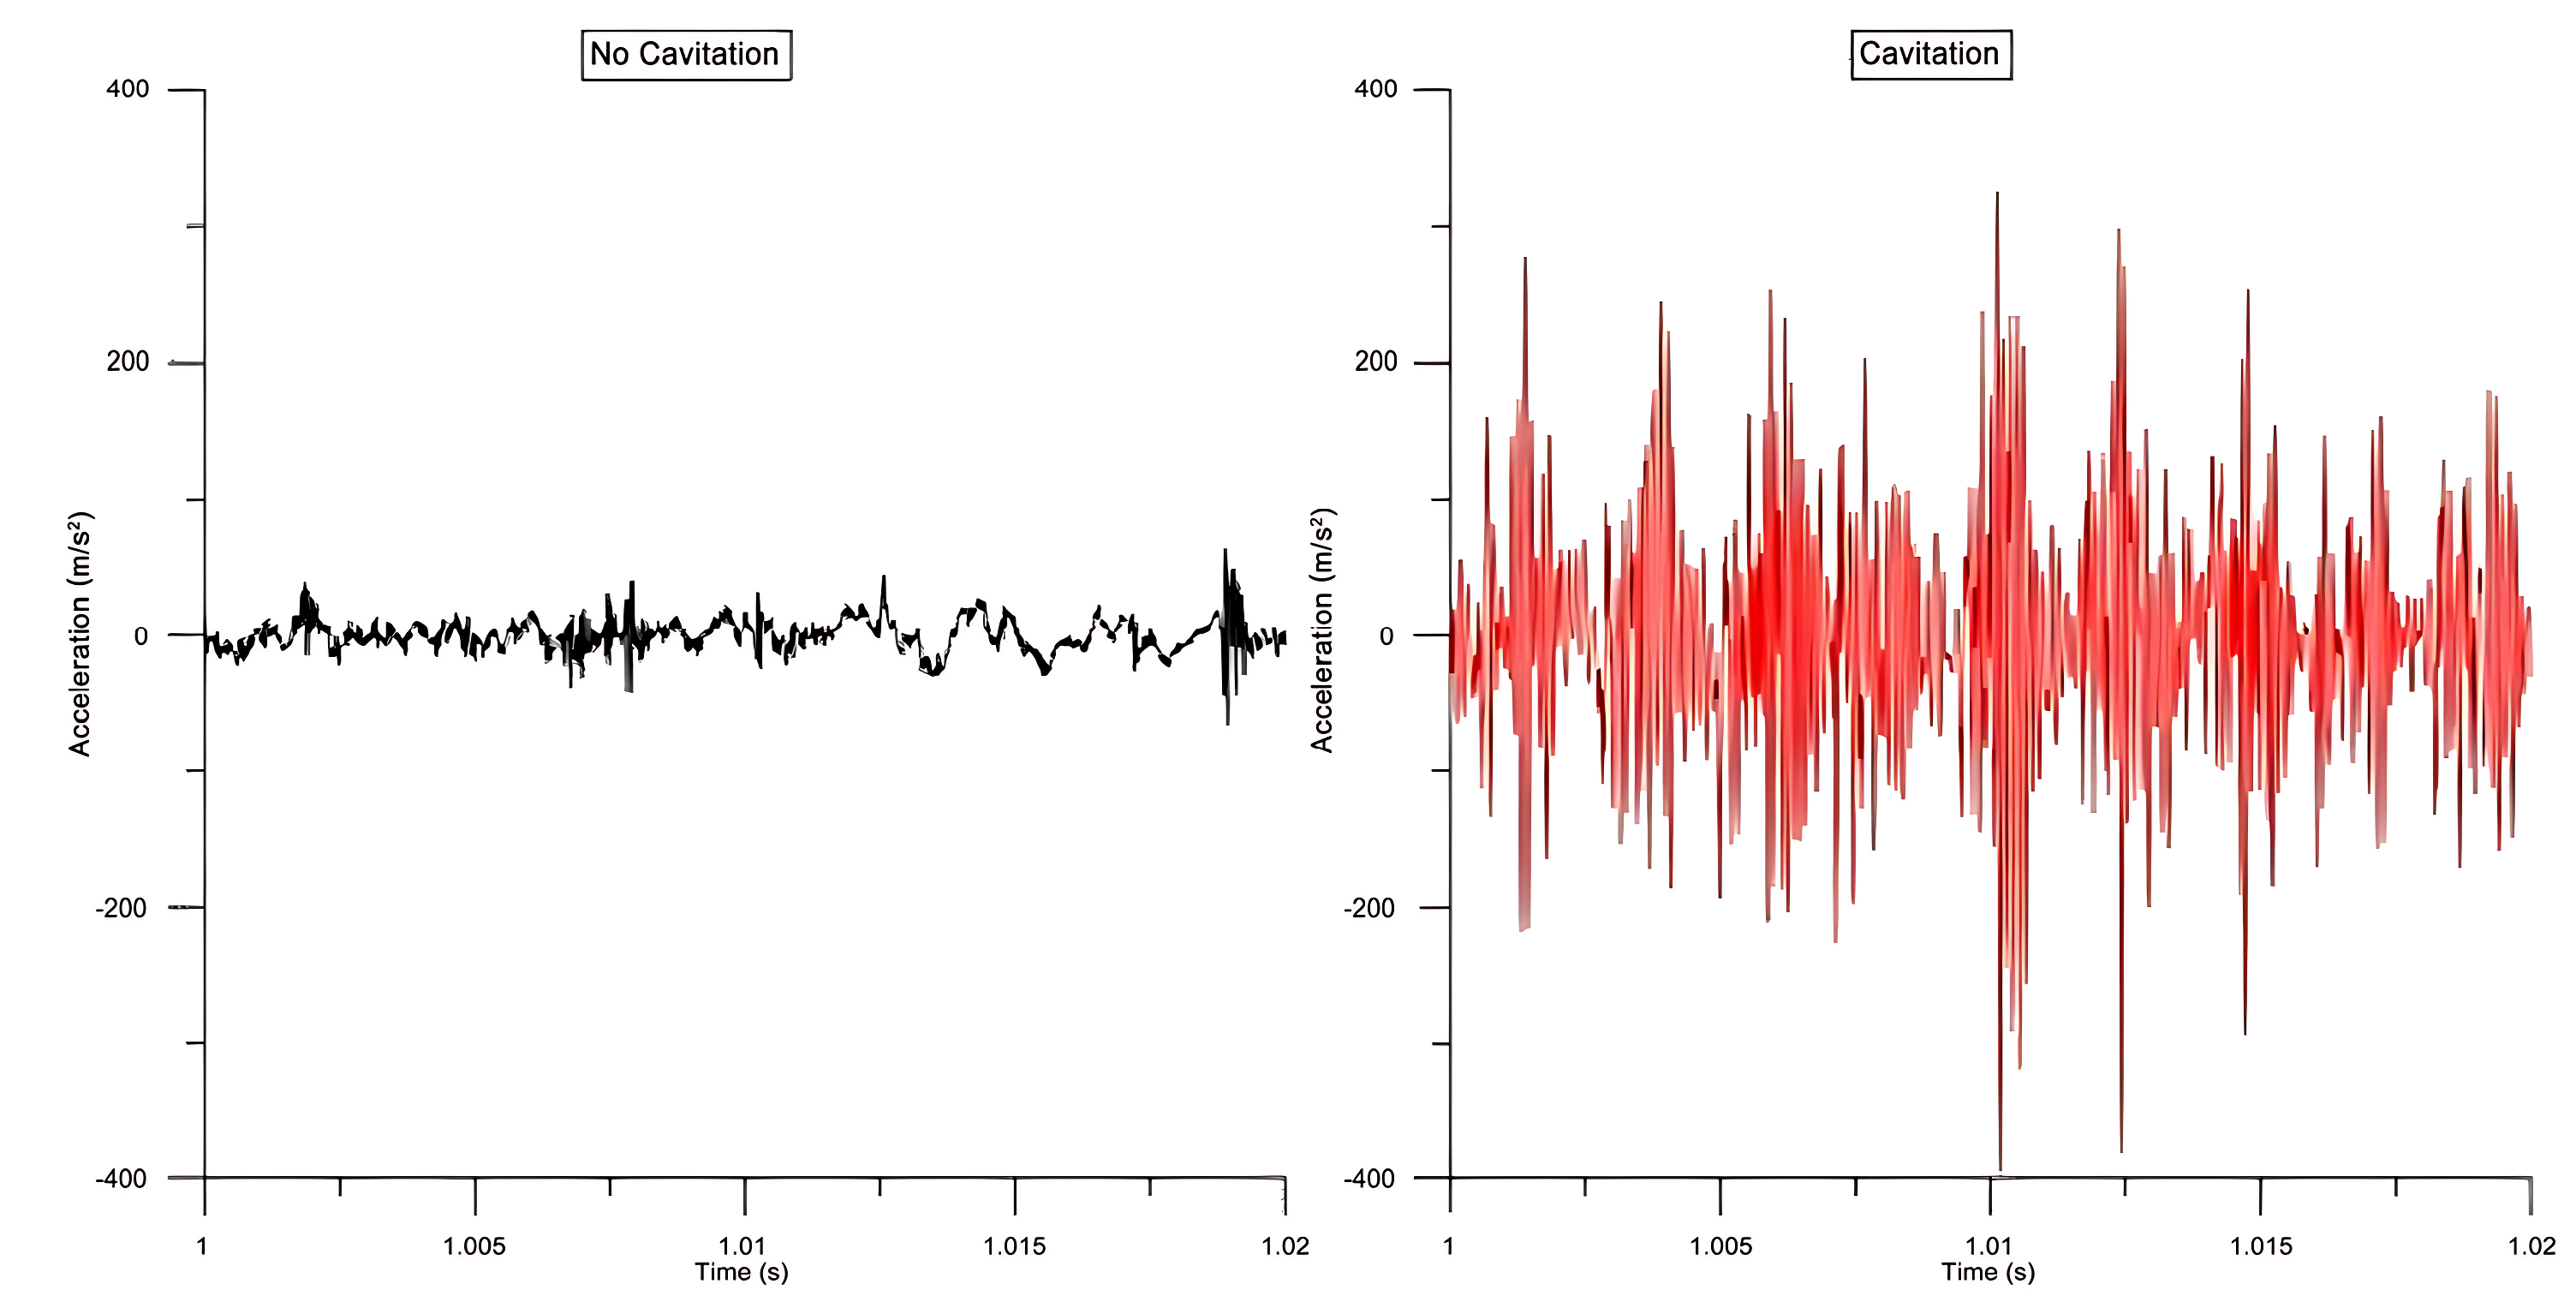
\includegraphics[width=0.95\linewidth]{figs//Artigos//Liu/Figura4A_Upscaler_2K.png}
    \caption{Sinais de aceleração no domínio do tempo em estados de cavitação e não cavitação. Fonte: \citeonline{liu2023review}}
    \label{fig:LiuFig4A}
\end{figure}

A Figura \ref{fig:LiuFig4A} apresenta os sinais de aceleração medidos em uma bomba centrífuga em duas condições distintas: à esquerda, operação normal (sem cavitação), e à direita, sob cavitação. Observa-se que o regime sem cavitação exibe um sinal estável, de baixa amplitude e com pequenas variações associadas ao ruído de fundo e às vibrações naturais da máquina. Em contrapartida, o regime cavitante demonstra um aumento expressivo na amplitude e na irregularidade temporal do sinal, reflexo direto do colapso das bolhas de vapor dentro do fluido. Esse comportamento errático é característico da cavitação e se intensifica com o aumento da velocidade de rotação e da severidade do fenômeno.

\begin{figure}[H]
    \centering
    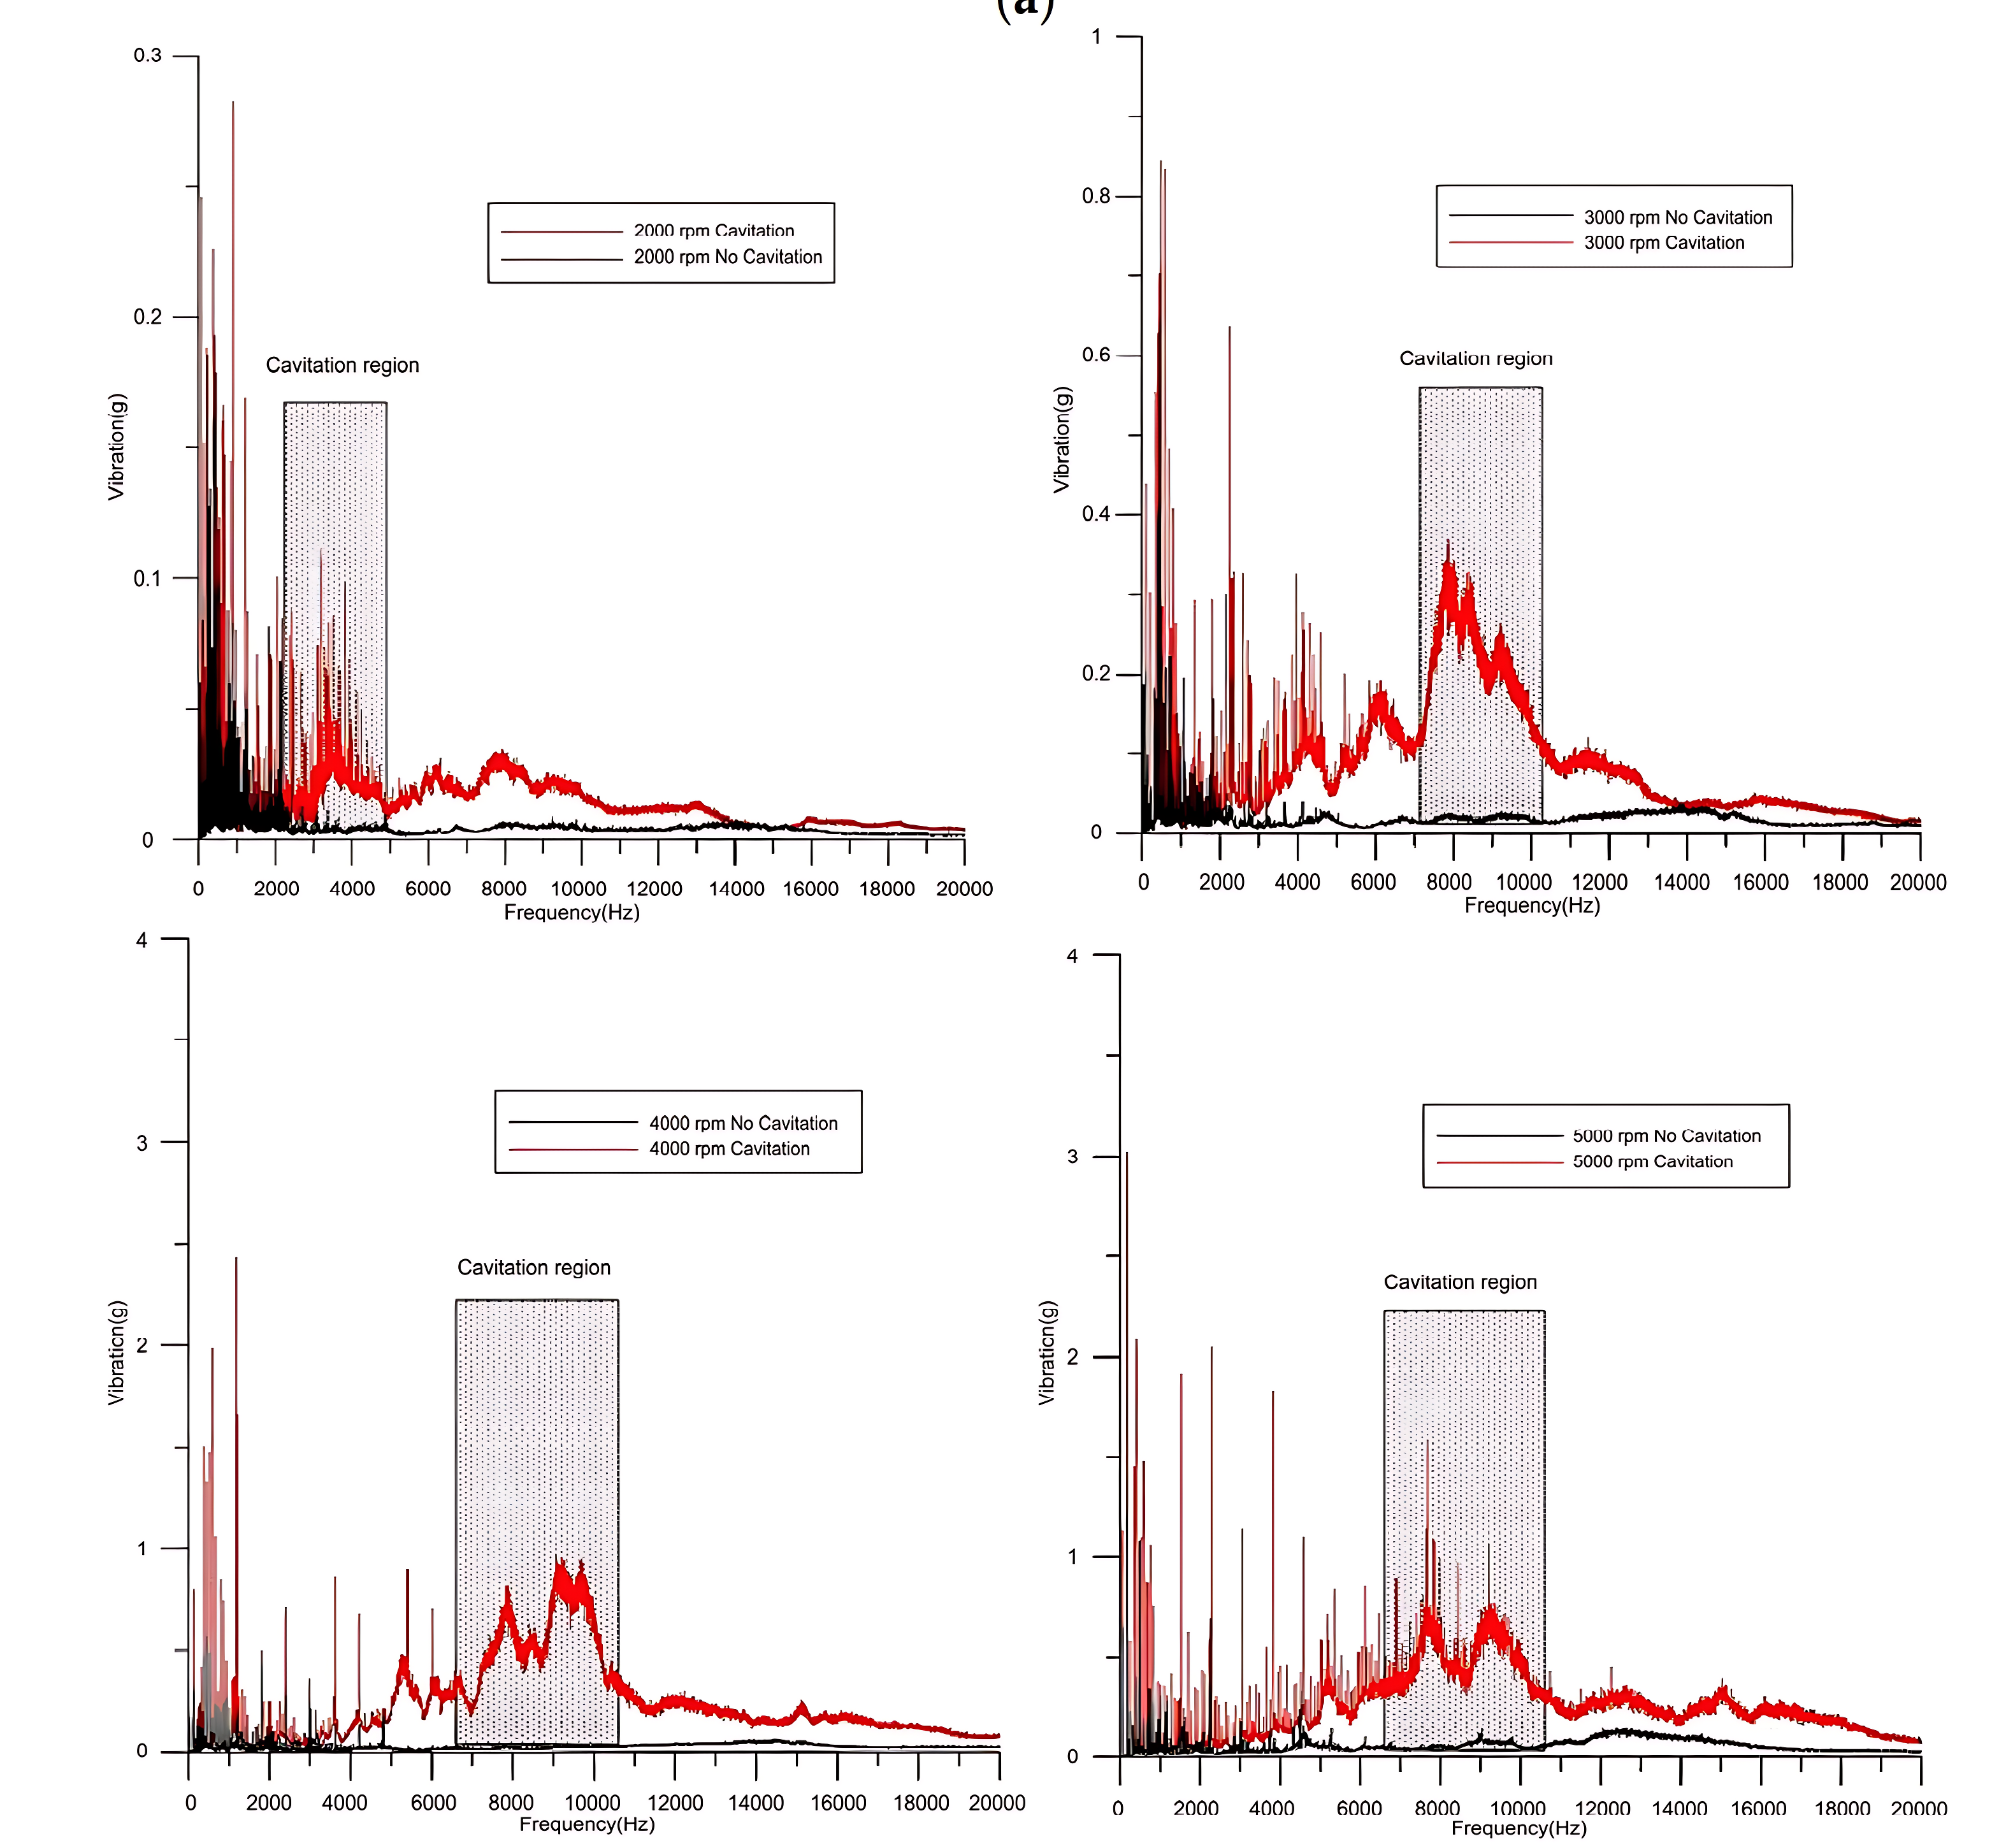
\includegraphics[width=0.95\linewidth]{figs//Artigos//Liu/Figura4B_Upscaler_4K.png}
    \caption{Espectro de sinal de vibração sob diferentes rpm. Fonte: \citeonline{liu2023review}}
    \label{fig:LiuFig4B}
\end{figure}

\linespread{1.27}\selectfont
Na Figura \ref{fig:LiuFig4B}, os sinais de vibração são analisados no domínio da frequência para diferentes velocidades de rotação (2000, 3000, 4000 e 5000 rpm). Os gráficos demonstram que, conforme a rotação aumenta, há um deslocamento e uma intensificação das componentes espectrais na faixa de 2 kHz a 8 kHz — região marcada como \textit{cavitation region}. Esses picos adicionais resultam da energia liberada pelos colapsos das bolhas de vapor, que introduzem novas componentes de alta frequência no espectro. A Figura \ref{fig:LiuFig4B} também mostra que a amplitude dessas componentes cresce com o aumento da rotação, evidenciando uma correlação direta entre a intensidade da cavitação e o conteúdo de alta frequência do sinal. Essa observação reforça a utilidade da análise espectral na \mbox{identificação e quantificação do fenômeno.}
\linespread{1.25}\selectfont

\begin{figure}[H]
    \centering
    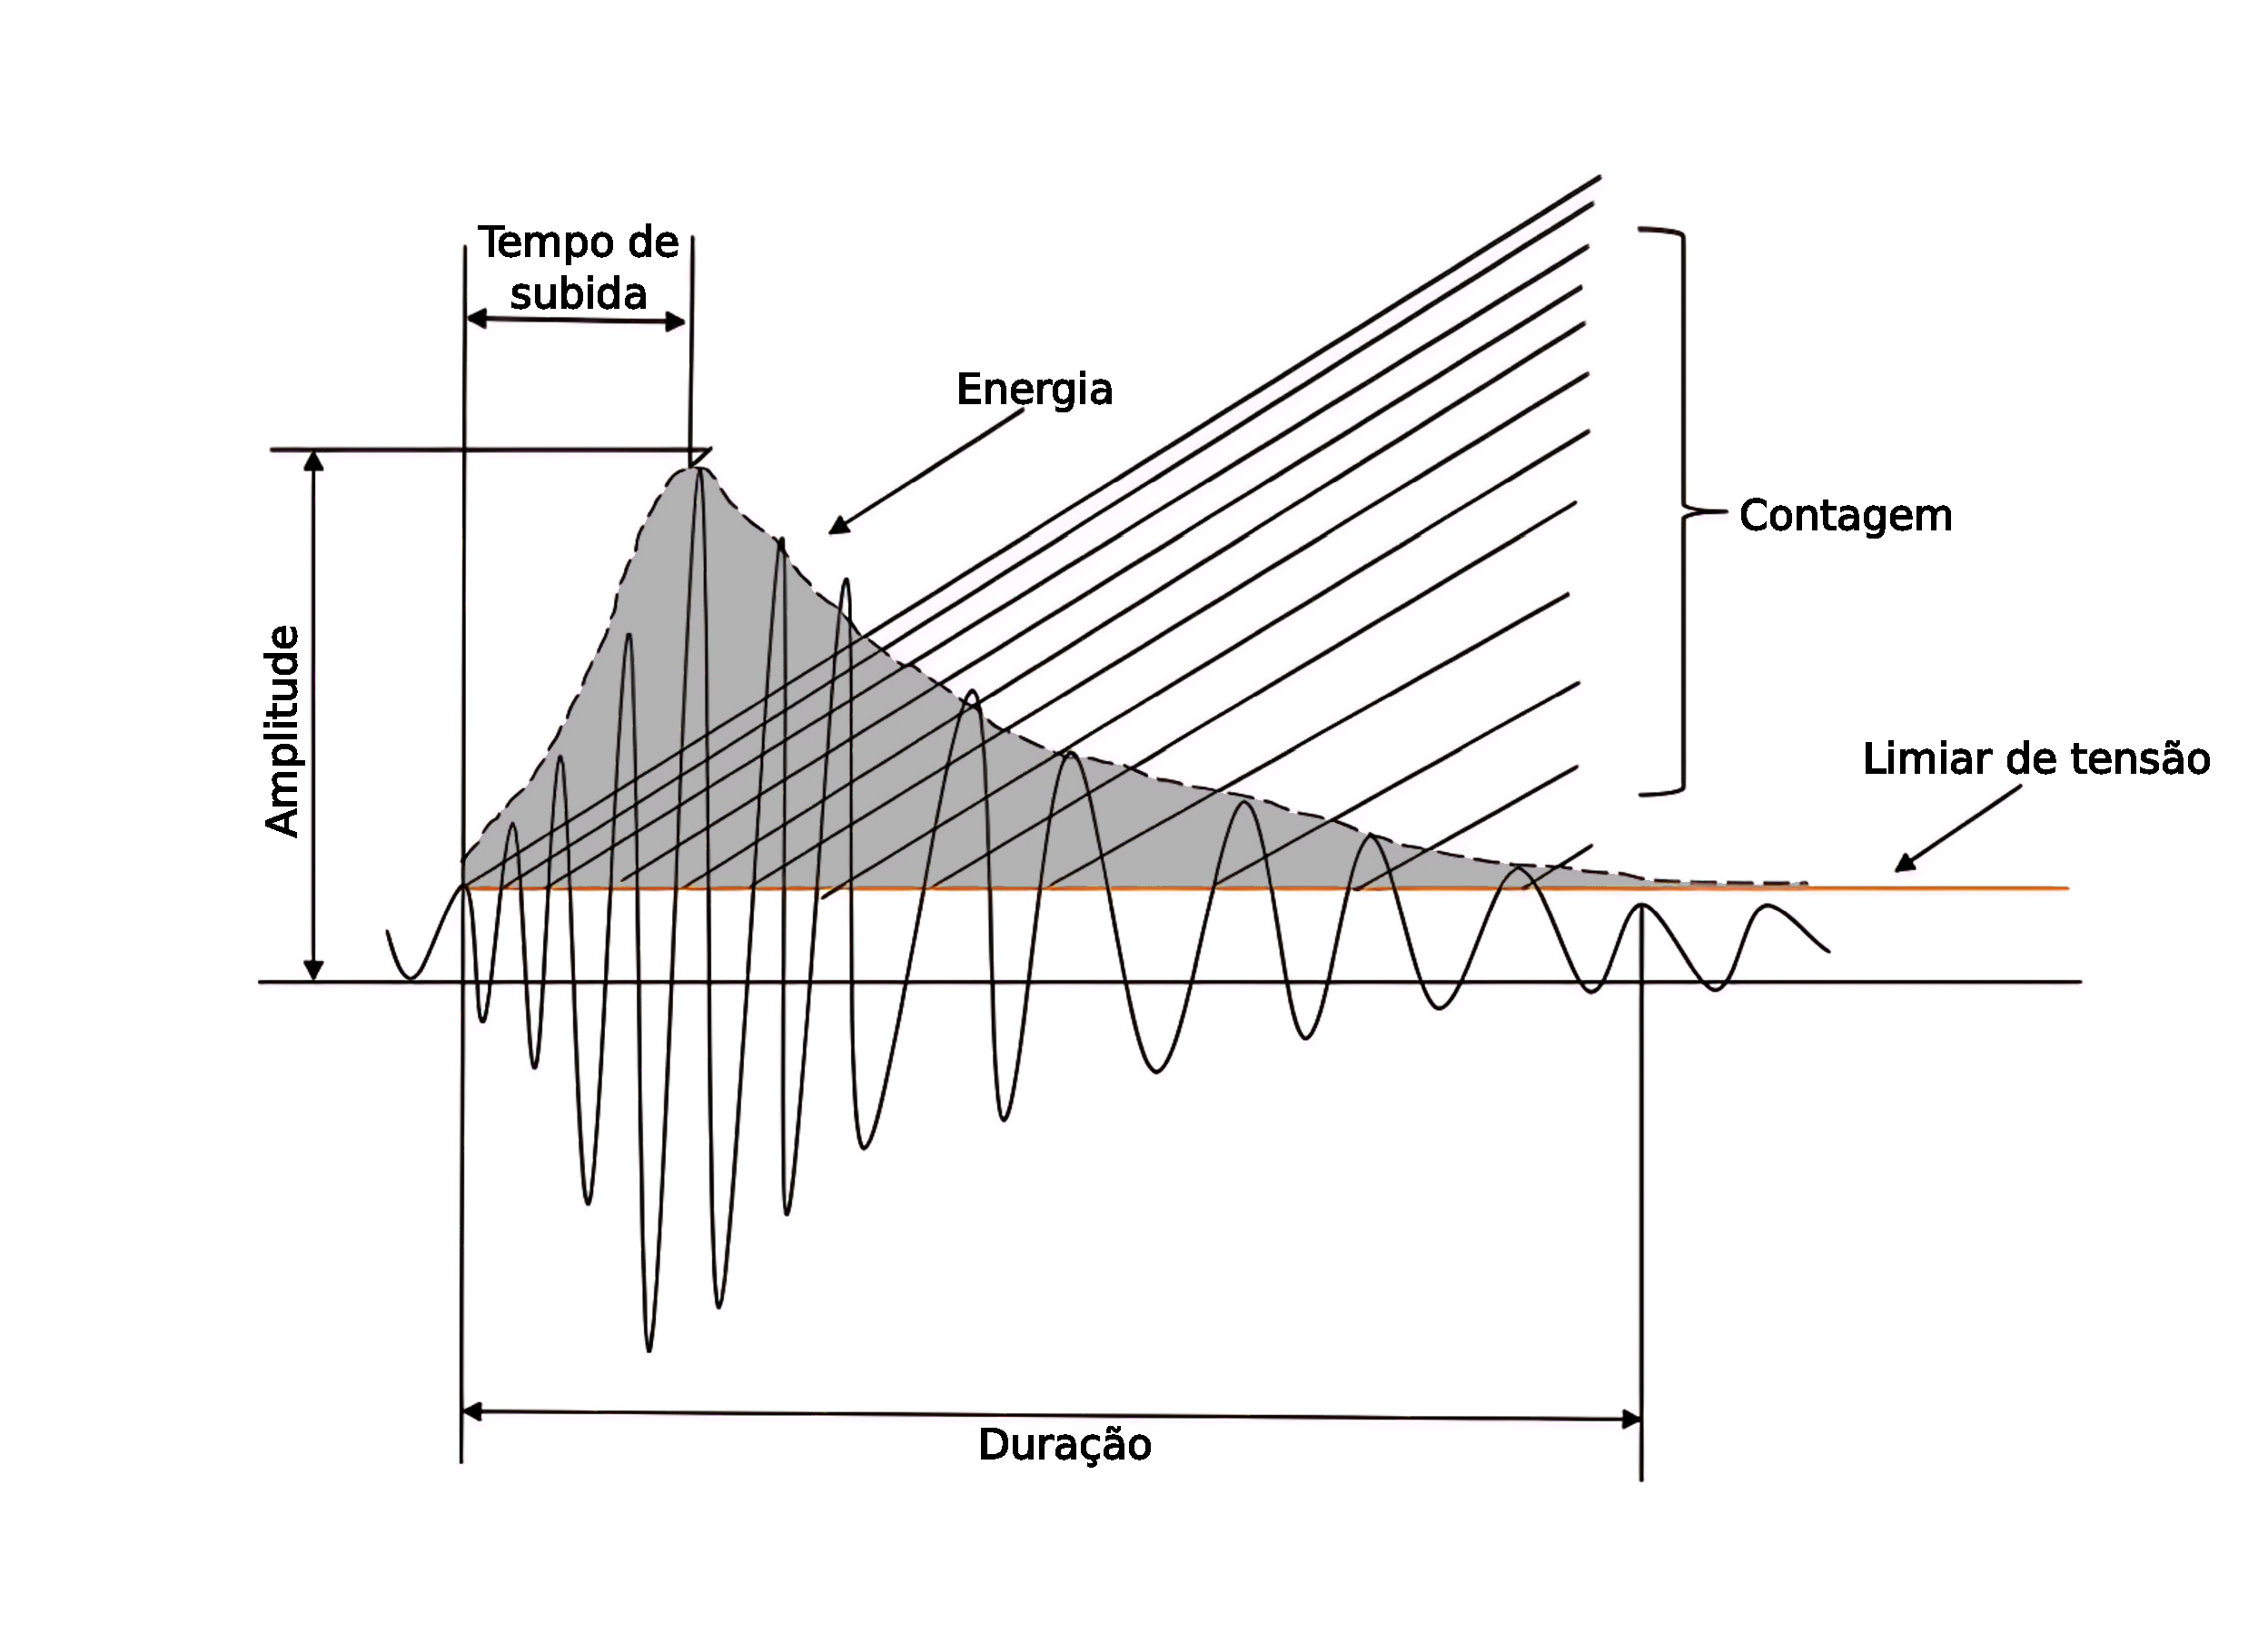
\includegraphics[width=0.9\linewidth]{figs//Artigos//Liu/Figura6.pdf}
    \caption{Parâmetros característicos do sinal de emissão acústica. Adaptado de  \citeonline{liu2023review}}
    \label{fig:LiuFig6}
\end{figure}

A Figura \ref{fig:LiuFig6} ilustra a decomposição de um evento típico de emissão acústica (“hit”) em seus principais parâmetros: amplitude, tempo de subida, \textit{rise time}, duração, energia e número de contagens acima do limiar, \textit{counts}. A amplitude representa o pico máximo do sinal, enquanto o tempo de subida corresponde ao intervalo entre o primeiro cruzamento do limiar e o pico máximo. A duração cobre o período total em que o sinal permanece acima do limiar, e a energia é obtida pela integral do sinal retificado. O número de contagens indica quantas vezes o sinal cruza o limiar estabelecido. Esses parâmetros são amplamente utilizados na caracterização de eventos de cavitação, pois refletem a intensidade e a frequência dos impactos associados ao colapso das bolhas, permitindo discriminar entre ruído e atividade cavitante real.

O ruído hidrodinâmico caracteriza-se por apresentar um espectro de banda larga e comportamento estocástico, resultante dos fenômenos de formação, crescimento e colapso de bolhas de vapor no interior do escoamento. Diferentemente do ruído mecânico, que tem natureza periódica e está associado a elementos estruturais da bomba (como mancais, rolamentos e pás do impulsor), o ruído hidrodinâmico reflete diretamente a instabilidade do fluido e as flutuações de pressão induzidas pela cavitação.

A Figura \ref{fig:LiuFig7}, adaptada de \citeonline{liu2023review}, apresenta a composição do ruído em bombas centrífugas, discriminando suas origens e mecanismos de formação. No topo, o ruído total da bomba, \textit{Pump noise} é dividido em dois grandes grupos: o ruído mecânico e o ruído hidrodinâmico. O primeiro engloba vibrações estruturais e ruídos discretos de frequência bem definida, como as frequências de passagem de pás e harmônicos, enquanto o segundo abrange componentes de ruído de cavitação, fluxo turbulento e separação de fluxo, de natureza predominantemente aleatória e de banda larga. Dentro do ruído de cavitação, por sua vez, distinguem-se componentes discretos e de banda larga, correspondentes a diferentes estágios e intensidades do fenômeno.

\begin{figure}[H]
\centering
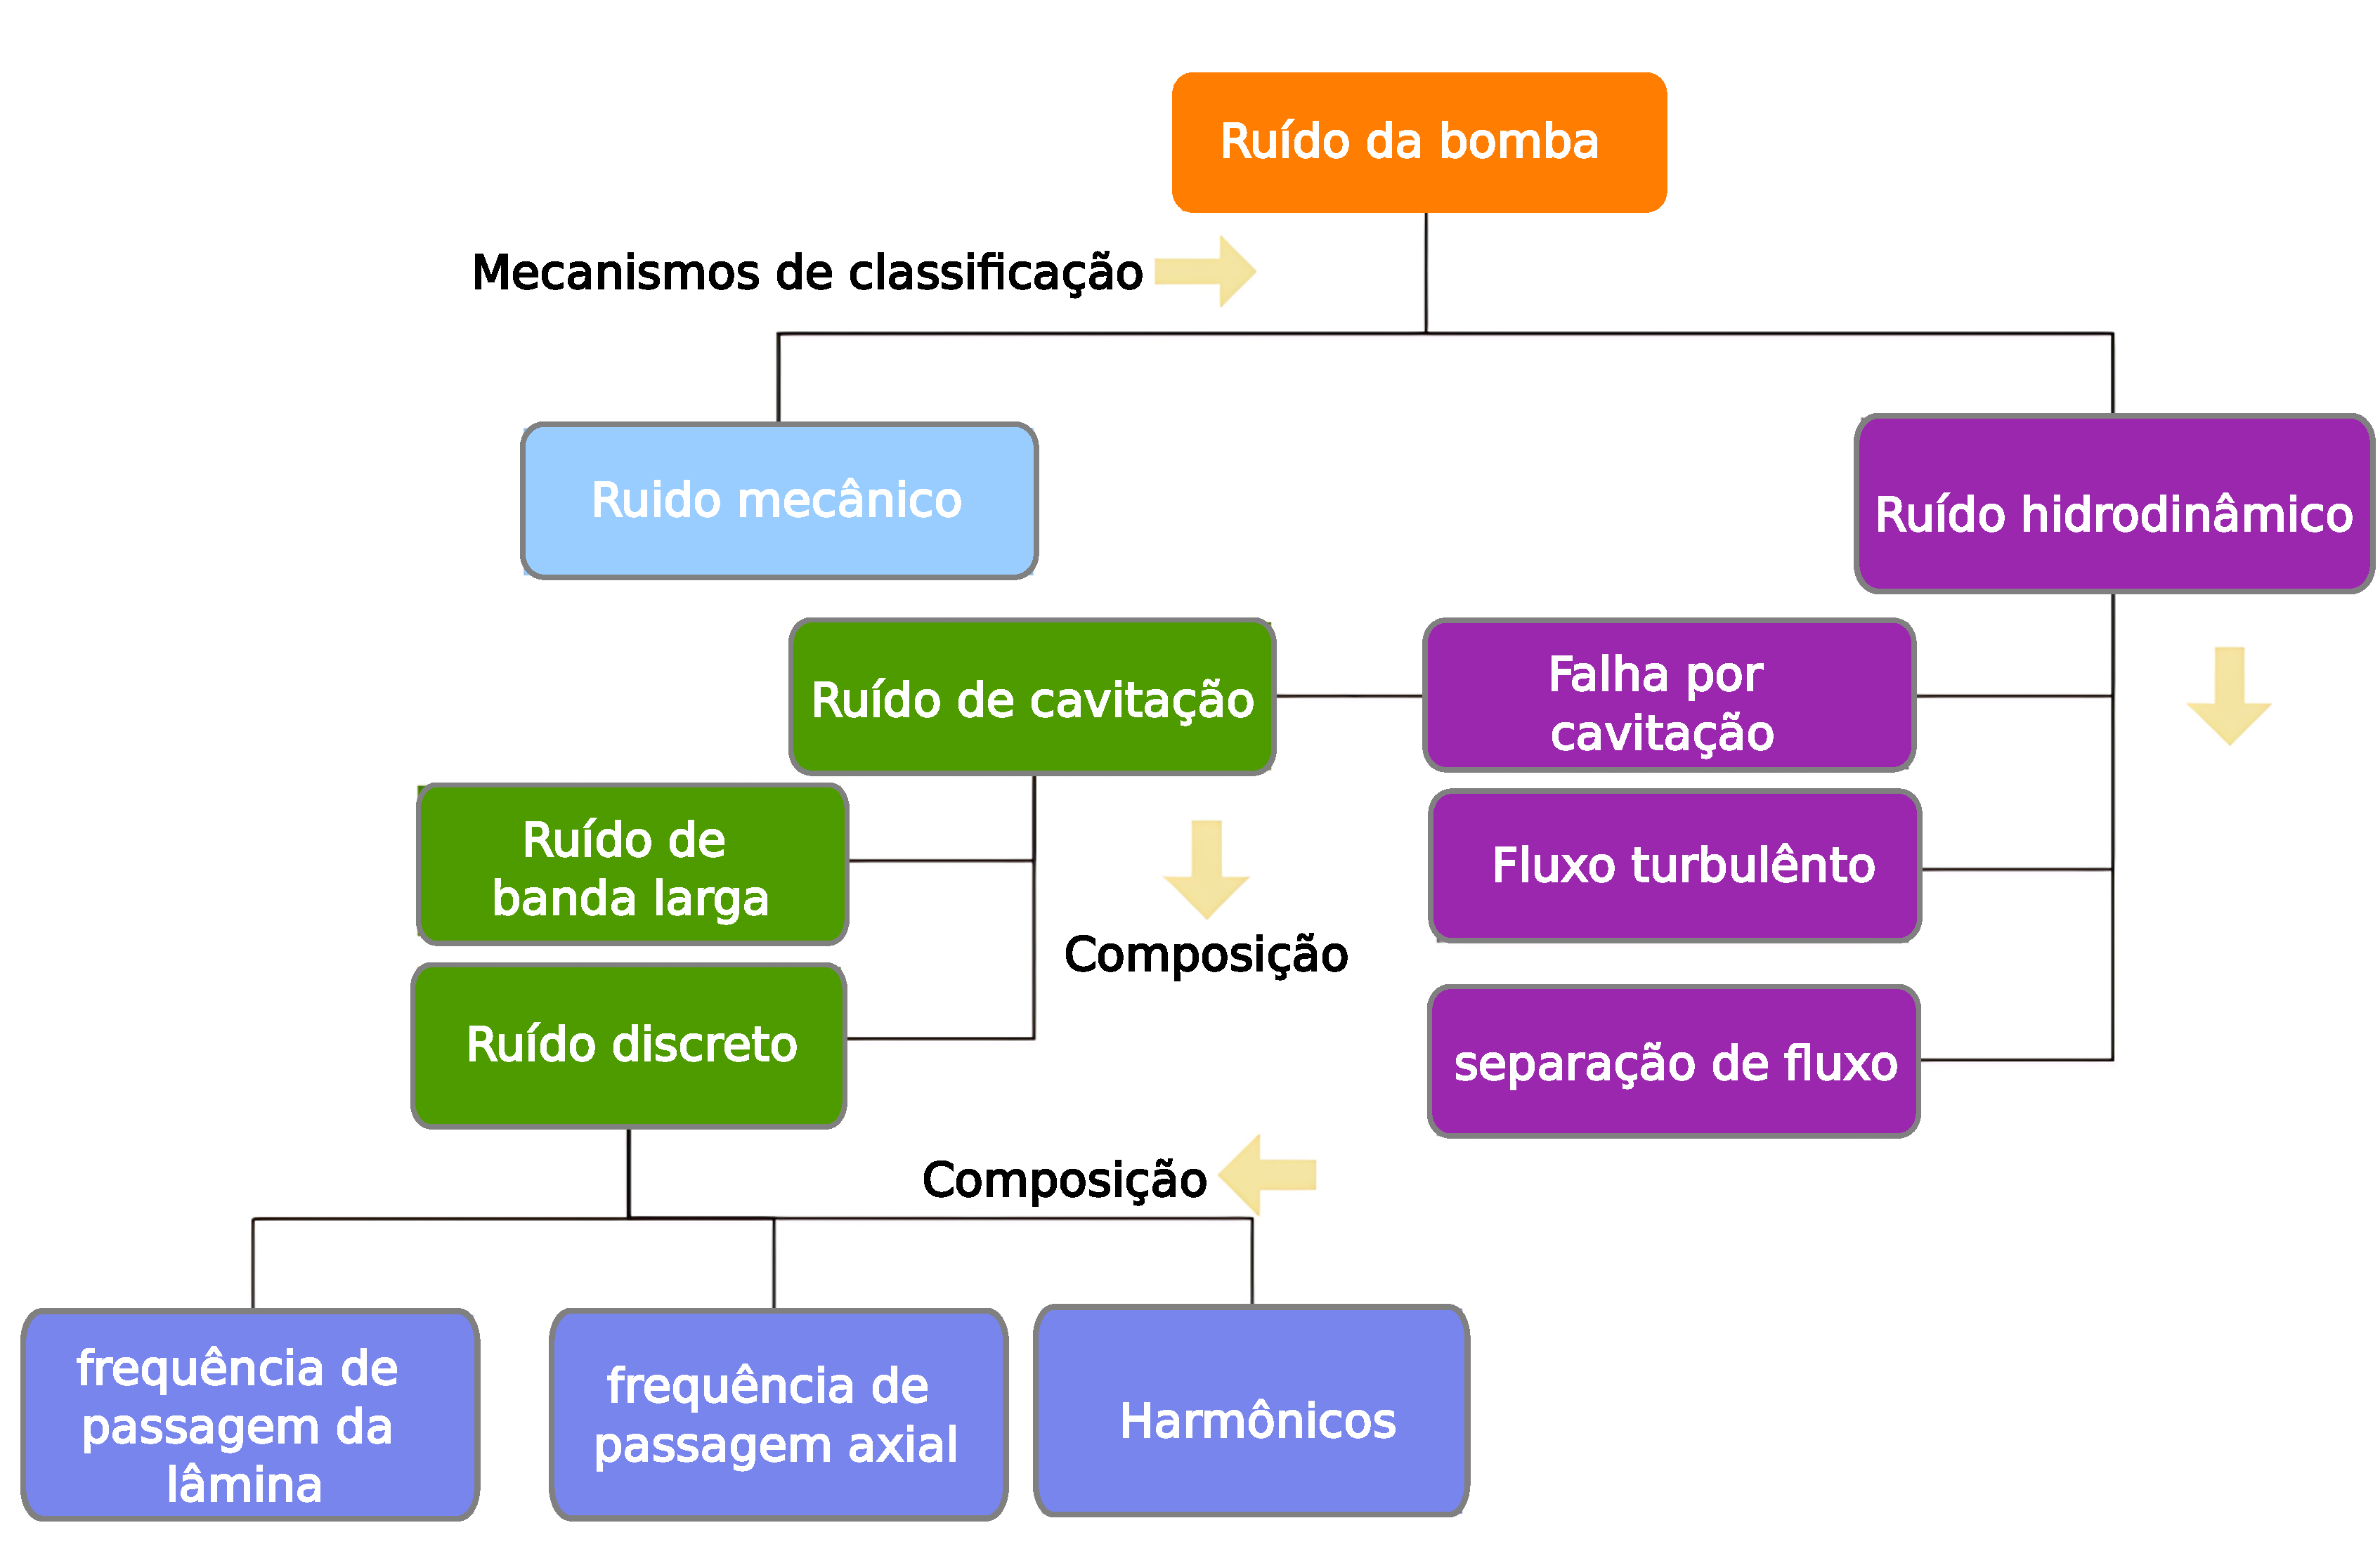
\includegraphics[width=0.75\linewidth]{figs//Artigos//Liu/Figura7.pdf}
\caption{Composição e mecanismos geradores do ruído em bombas centrífugas. Adaptado de \citeonline{liu2023review}.}
\label{fig:LiuFig7}
\end{figure}

Essa técnica de análise de ruído é particularmente útil em ensaios laboratoriais e ambientes controlados, nos quais as fontes de interferência externa podem ser minimizadas. Todavia, em aplicações industriais, sua eficácia tende a ser reduzida devido à forte influência de ruídos ambientais e à dificuldade de isolar as componentes específicas~associadas~à~cavitação.

Em contrapartida, o método baseado na pulsação de pressão apresenta maior robustez frente a interferências, uma vez que mede diretamente as variações de pressão no fluido, refletindo as flutuações hidráulicas e a eficiência volumétrica do sistema. Seu principal inconveniente, entretanto, é a natureza invasiva da instrumentação, que requer conexão física com o circuito hidráulico, além de uma baixa sensibilidade temporal para eventos de curta duração — o que limita sua capacidade de detectar a cavitação incipiente.

De modo comparativo, \citeonline{liu2023review} destacam que a emissão acústica e o ruído hidrodinâmico se sobressaem na detecção inicial da cavitação, enquanto a vibração é amplamente utilizada pela maturidade teórica e a pulsação de pressão pela robustez e simplicidade de implementação. As tendências futuras apontam para a convergência entre sensores de alta sensibilidade e métodos modernos de processamento de sinais não estacionários, aliada ao uso de inteligência artificial, em especial redes neurais convolucionais e aprendizado por reforço profundo, \mbox{para extração de padrões e detecção automatizada.}

Em síntese, a revisão conduzida por \citeonline{liu2023review} reforça que a emissão acústica permanece como uma das técnicas mais promissoras para a detecção precoce da cavitação, ainda que sua ampla adoção dependa de avanços em aspectos técnicos e econômicos, incluindo a redução de custos dos sensores piezoelétricos, a integração com hardware embarcado e o desenvolvimento de algoritmos otimizados para análise em tempo real.

\citeonline{poddar2021classification} apresentam um estudo voltado à detecção de falhas incipientes em mancais hidrodinâmicos, \textit{journal bearings}, investigando simultaneamente sinais EA e de vibração. Os autores ressaltam que fenômenos como cavitação, contaminação por partículas e falta de lubrificação são causas relevantes de degradação na performance de mancais, podendo levar à erosão, perda de eficiência e falhas prematuras. Neste contexto, métodos que permitam a identificação precoce dessas condições assumem papel crucial em estratégias de manutenção preditiva.

O experimento baseia-se em um arranjo monitorado, onde sensores de vibração e sensores de emissão acústica foram instalados em um mancal submetido a diferentes condições operacionais — incluindo variações no regime de carga, contaminação por partículas de diferentes tamanhos e situações de lubrificação insuficiente. O objetivo central consistiu em comparar a sensibilidade das duas técnicas, especialmente no que tange à detecção da cavitação incipiente. Os sinais coletados foram processados nos domínios do tempo e da frequência, a partir dos quais foram extraídos parâmetros como RMS, fator de crista, amplitude de pico, energia acumulada e número de contagens (no caso da EA). A análise foi estendida ao domínio tempo-frequência para capturar a \mbox{evolução espectral dos fenômenos de falha.}

Os resultados demonstram que os sinais de vibração apresentaram alterações significativas apenas em estágios mais avançados dos defeitos, quando ocorreram instabilidades acusadas no escoamento ou deterioração clara da película hidráulica. Em contraste, os sinais de emissão acústica revelaram-se muito mais sensíveis em estágios iniciais; observou-se, por exemplo, crescimento progressivo dos parâmetros energia acumulada e número de contagens com o agravamento da condição, o que evidencia uma correlação direta com os eventos de colapso de bolhas ou microcontatos. Os autores também apontam que amplitude e largura de banda dos sinais EA expandem-se de modo notável sob condições de falha — enquanto os índices de vibração \mbox{mantêm-se relativamente estáveis.}

A discussão conclui que a técnica de emissão acústica apresenta desempenho claramente superior na detecção precoce da cavitação e de deteriorações relacionadas, pois consegue identificar alterações no regime de escoamento antes mesmo que se verifique qualquer impacto mensurável no desempenho hidrodinâmico global do equipamento. A análise vibracional, embora útil, tende a ser mais responsiva em estágios posteriores da falha, quando modificações estruturais ou oscilações adicionais já se refletem na resposta dinâmica do conjunto. Do ponto de vista metodológico, o estudo indica que a integração entre ambas as abordagens pode enriquecer o diagnóstico, ampliando a compreensão do processo de degradação. Contudo, mesmo sem recorrer a medições complementares, a EA já se mostra como a alternativa mais sensível e promissora para a identificação incipiente de cavitação, conforme evidenciado em \citeonline{poddar2021classification}.

\citeonline{amini2022development} apresentam o desenvolvimento de um sistema inovador para o monitoramento da cavitação em turbinas hidráulicas, fundamentado na análise de sinais acústicos aliada a algoritmos de aprendizado de máquina. Os autores apontam que a operação de turbinas em condições fora do ponto ótimo de eficiência aumenta a probabilidade de ocorrência de cavitação, o que por sua vez acarreta degradação de desempenho, vibrações estruturais e, principalmente, danos mecânicos por erosão. Nesse sentido, a proposta busca oferecer uma ferramenta não intrusiva, capaz de detectar tanto a ocorrência quanto a severidade do fenômeno em tempo real, contribuindo para a manutenção preditiva em centrais hidrelétricas.

A metodologia foi organizada em duas fases distintas. Na primeira, foram realizados experimentos controlados no túnel de cavitação da HES-SO Valais/Wallis, em que se utilizou um hidrofólio de aço inoxidável do tipo NACA 0015 para induzir a cavitação em condições estáticas e dinâmicas, conforme ilustrado na Figura \ref{fig:amini2022developmentFig1}. Nessa etapa, o ruído no aerofólio foi registrado por meio de um microfone GRAS 46 AE com frequência de amostragem de 40 kHz, e os sinais foram analisados nos domínios temporal e espectral. Em uma segunda fase, a técnica foi validada em escala real na usina hidrelétrica de Ernen, no cantão de Valais (Suíça), equipada com turbinas Francis de 16 MW cada, como mostra a Figura \ref{fig:amini2022developmentFig2}. Durante essa campanha experimental, foram simuladas diferentes condições operacionais, abrangendo variações de carga, níveis de jusante e introdução de ruídos artificiais, com o intuito de avaliar a robustez do sistema.

\begin{figure}[H]
    \centering
    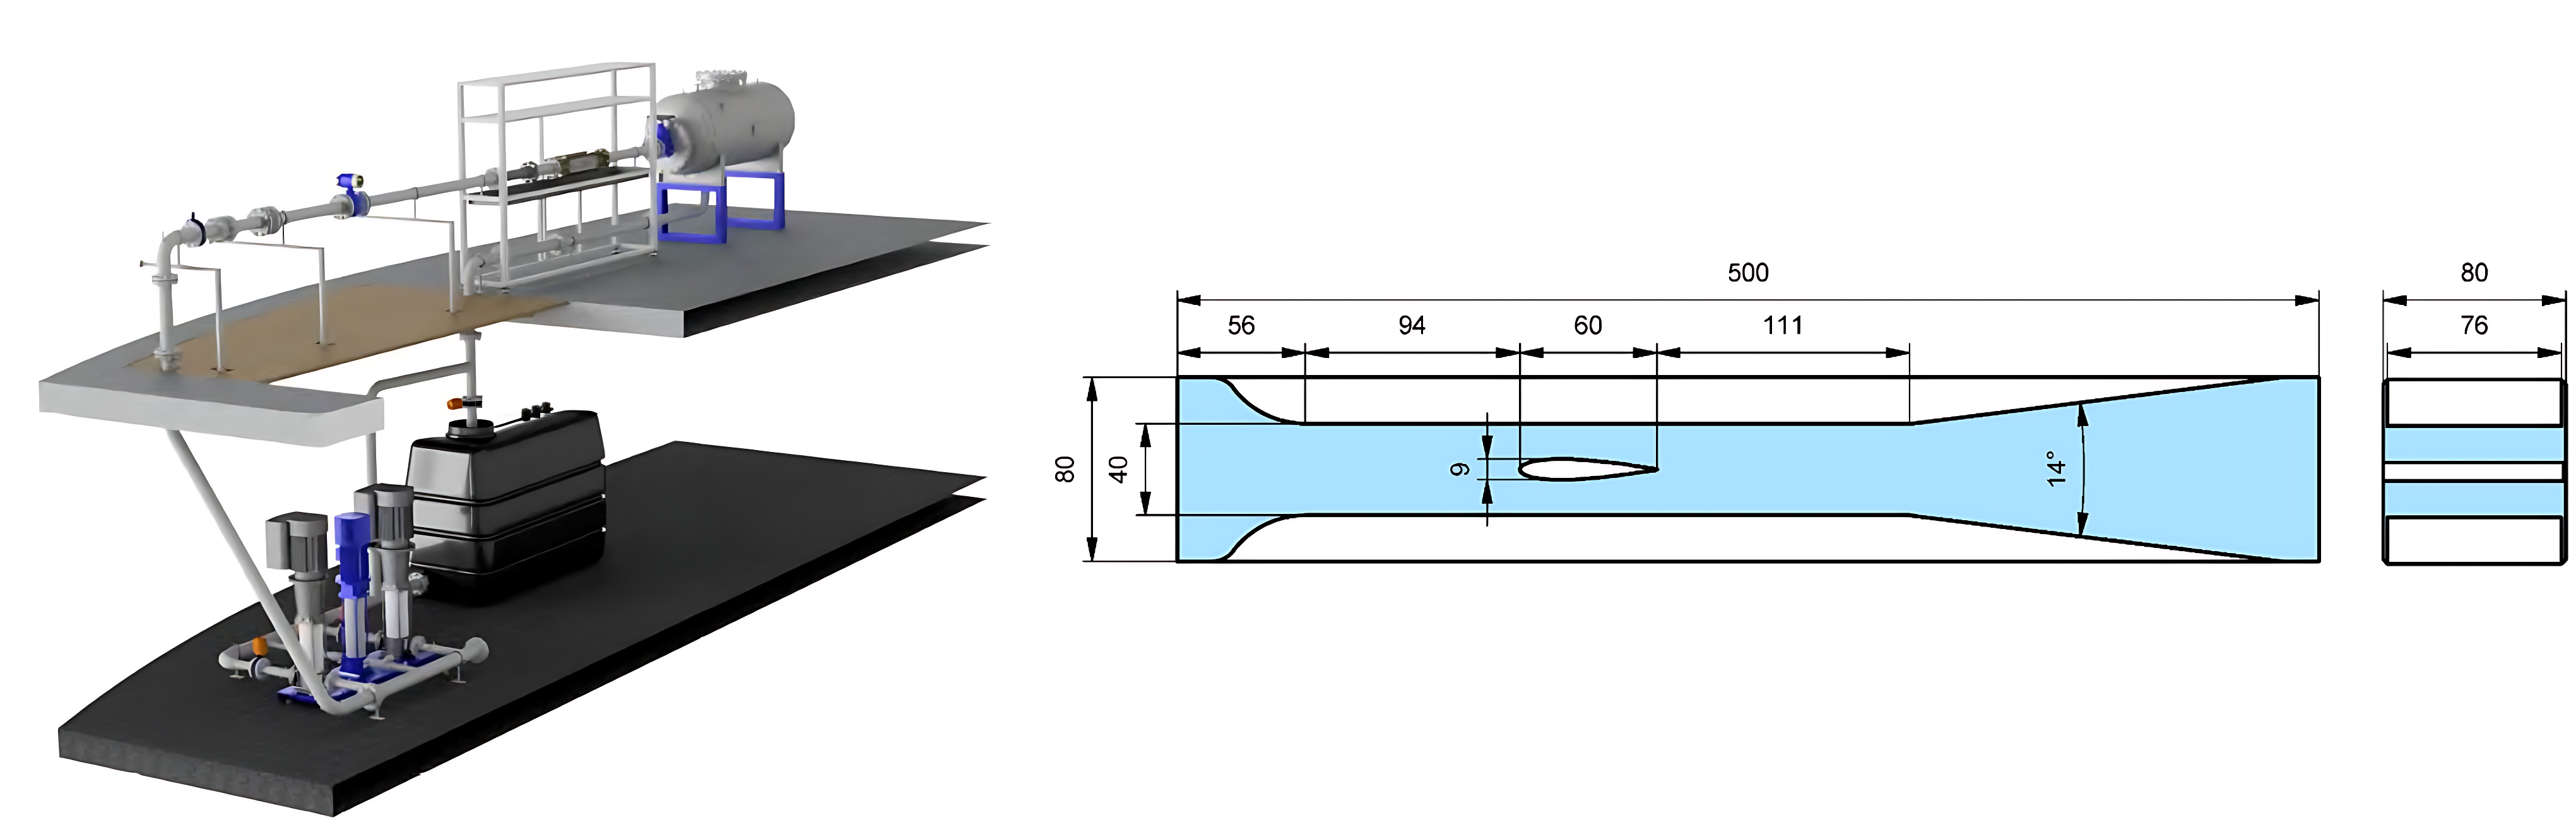
\includegraphics[width=1.0\linewidth]{figs/Artigos/amini2022development/Figura1_Upscaler_2K.png}
    \caption{(À esquerda) esquema do túnel de cavitação da HES-SO Valais/Wallis; (À direita) seção transversal do hidrofólio de aço inoxidável NACA 0015 testado. Fonte: \citeonline{amini2022development}}
    \label{fig:amini2022developmentFig1}
\end{figure}

\begin{figure}[H]
    \centering
    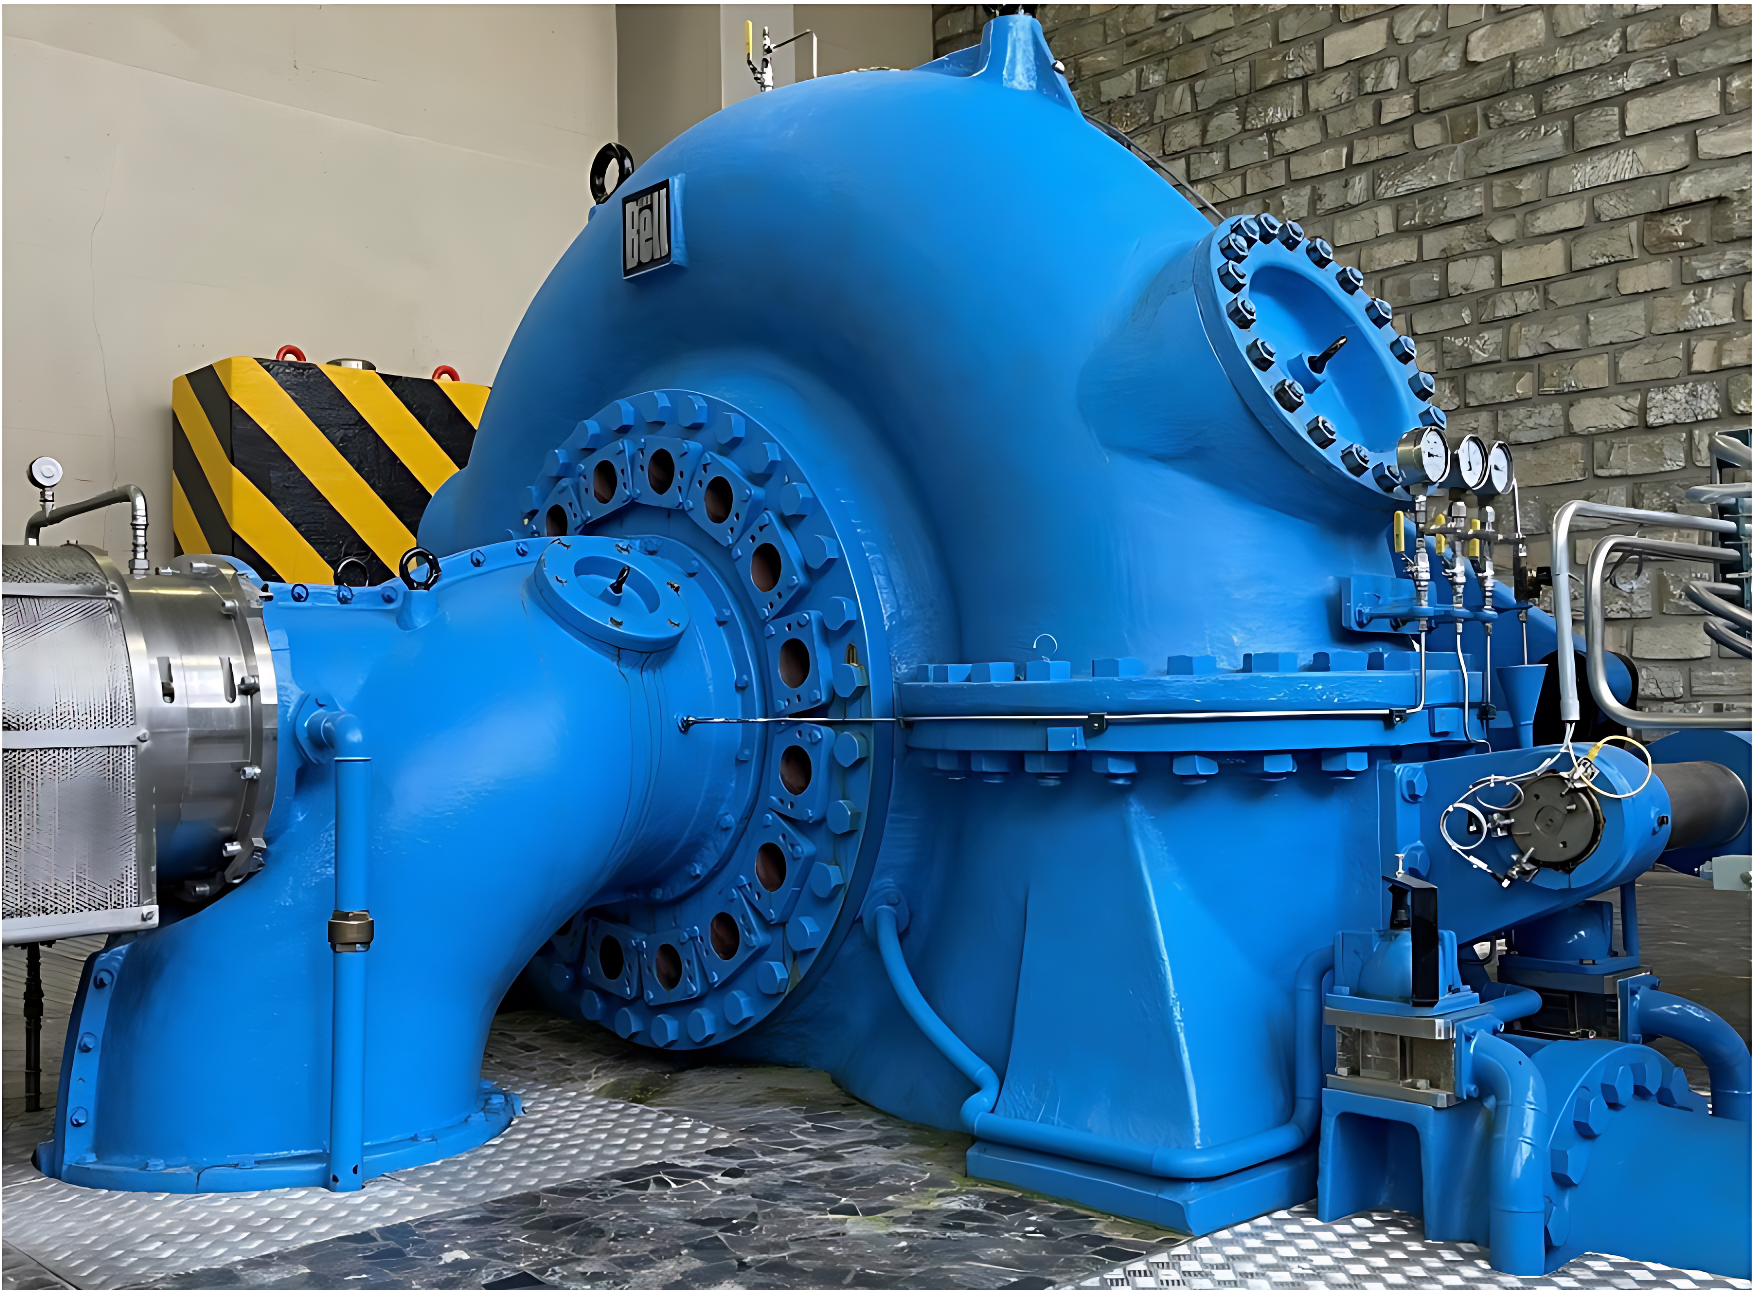
\includegraphics[width=.85\linewidth]{figs/Artigos/amini2022development/Figura2_Upscaler_2K.png}
    \caption{Turbina Francis de dois rotores na usina hidrelétrica de Ernen (Wallis, Suíça). Fonte: \citeonline{amini2022development}}
    \label{fig:amini2022developmentFig2}
\end{figure}

\linespread{1.27}\selectfont
As figuras explicam por si o salto metodológico:  
Figura \ref{fig:amini2022developmentFig1}: ilustra a instalação experimental de bancada no túnel de cavitação, onde o hidrofólio NACA 0015 foi submetido a perfis de escoamento com pressão de sucção reduzida para induzir cavitação. O desenho da seção transversal do hidrofólio permite visualizar as dimensões e geometria usadas nos testes. Essa figura demonstra claramente a etapa de laboratório, onde as condições são controladas, permitindo análise precisa dos sinais acústicos captados.

Figura \ref{fig:amini2022developmentFig2}: apresenta a aplicação em campo real, com uma turbina Francis de dois rotores na usina de Ernen. Essa imagem reforça a transição da metodologia do laboratório para o ambiente operacional industrial, destacando a compatibilidade da solução desenvolvida com sistemas de grande escala. A capacidade de validação em usina real confere maior credibilidade à técnica proposta.  

Em resumo, o estudo reforça a viabilidade do uso de sinais acústicos não invasivos em combinação com algoritmos de aprendizado para o monitoramento da cavitação em turbinas hidráulicas. A abordagem — centrada em microfones, processamento de sinais e classificação supervisionada — fornece uma estrutura promissora para aplicações industriais, o que dialoga diretamente com o foco desta dissertação: a implementação simulada de uma rede neural de convolução (CNN-1D) em hardware reconfigurável (FPGA) para detecção de falhas em sistemas hidráulicos.

\linespread{1.27}\selectfont
O processamento dos sinais foi realizado por meio da transformada rápida de Fourier (FFT) e da extração de características no domínio da frequência, com o objetivo de identificar padrões representativos da cavitação. Para a etapa de classificação supervisionada, foram testados dois algoritmos de aprendizado de máquina: o \textit{k-Nearest Neighbors} (k-NN), aplicado aos ensaios laboratoriais, e o \textit{Gaussian Mixture Model} (GMM), utilizado para os dados coletados na usina. 

Os resultados mostraram que, em condições estáticas de laboratório, a distinção entre regimes cavitantes e não cavitantes foi clara, atingindo 100\% de acurácia. Já nos ensaios dinâmicos, a precisão manteve-se elevada, superior a 95\%, mesmo diante da maior complexidade imposta pela rotulagem de dados e pela ausência de critérios visuais diretos para validação, como ilustram as Figuras~\ref{fig:amini2022developmentFig3} e~\ref{fig:amini2022developmentFig4}. Na aplicação em escala real, apesar da presença de ruído de fundo significativo, o algoritmo manteve desempenho consistente, separando com clareza as diferentes classes de operação e identificando distintos níveis de severidade da cavitação, conforme apresentado na Figura~\ref{fig:amini2022developmentFig6}.

\begin{figure}[H]
    \centering
    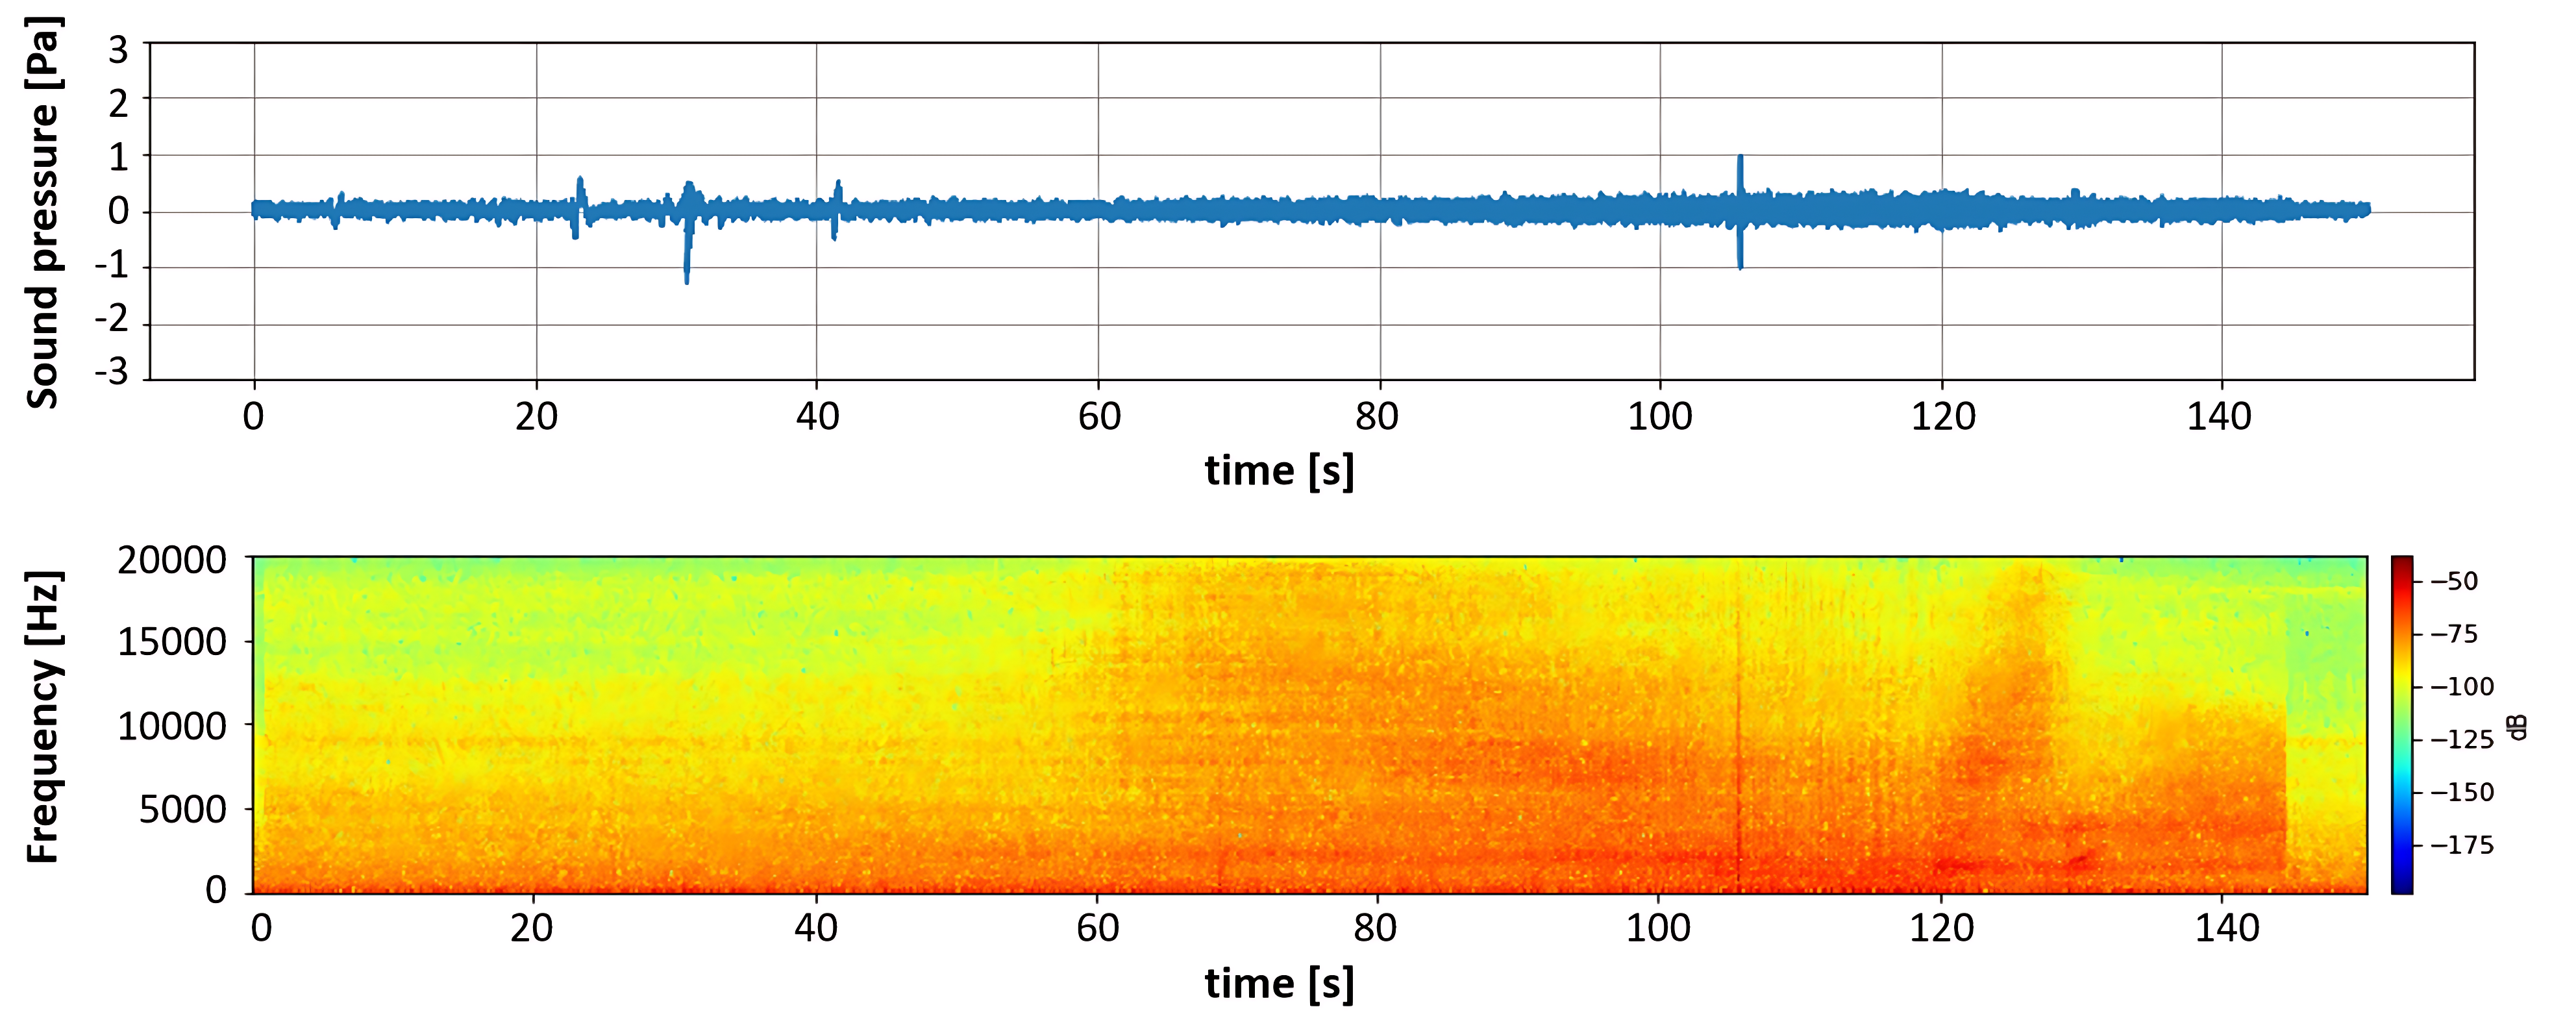
\includegraphics[width=1.0\linewidth]{figs/Artigos/amini2022development/Figura3_Upscaler_2K.png}
    \caption{Sinal acústico de um teste dinâmico ilustrado nos domínios de tempo (acima) e de frequência (abaixo). Fonte: \citeonline{amini2022development}}
    \label{fig:amini2022developmentFig3}
\end{figure}

\linespread{1.27}\selectfont
A Figura~\ref{fig:amini2022developmentFig3} apresenta o sinal acústico registrado durante um teste dinâmico. A parte superior mostra a variação da pressão sonora no tempo, enquanto o espectrograma inferior exibe a distribuição de energia no domínio da frequência. É possível observar o aumento de componentes de alta frequência à medida que a cavitação se intensifica, evidenciando a sensibilidade do método acústico.
\linespread{1.25}\selectfont

\begin{figure}[H]
    \centering
    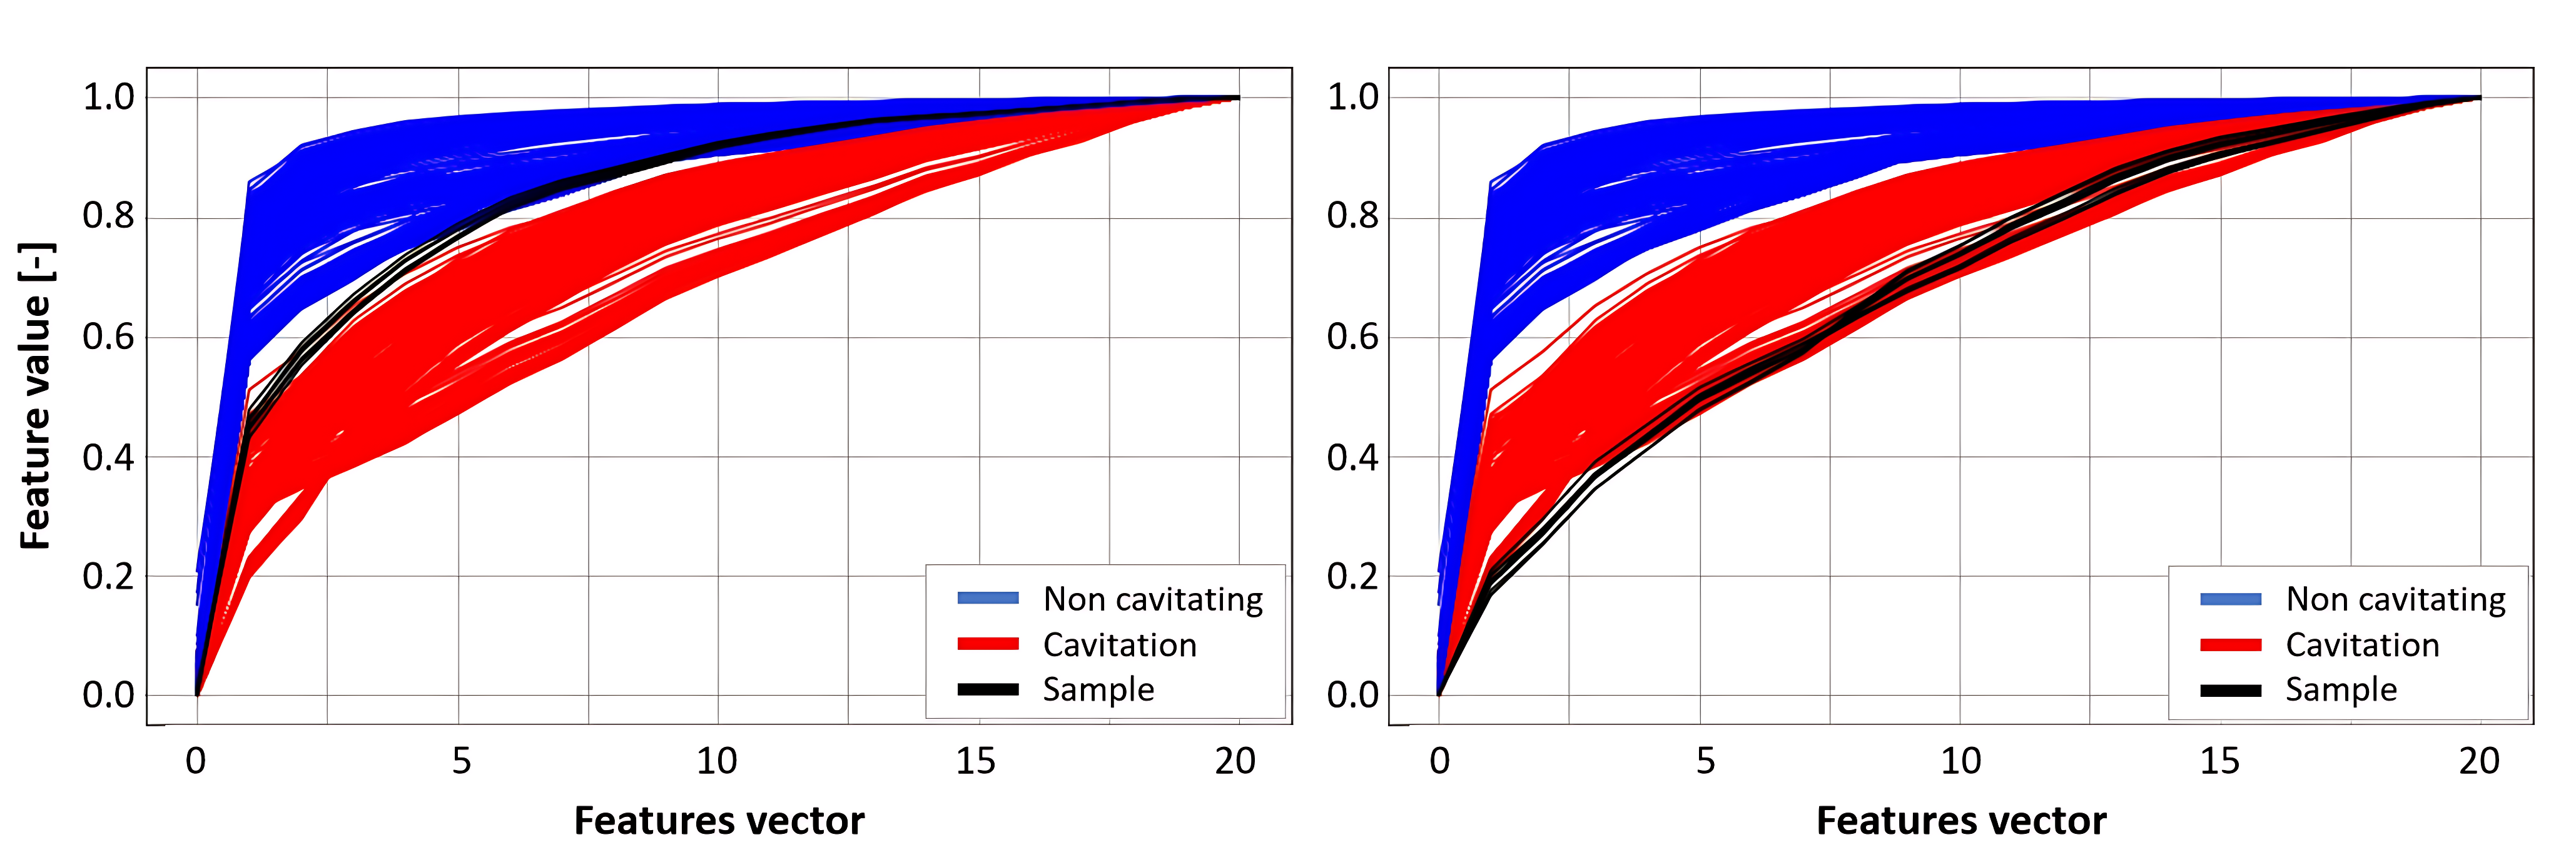
\includegraphics[width=1.0\linewidth]{figs/Artigos/amini2022development/Figura4_Upscaler_2K.png}
    \caption{Distribuição dos valores característicos extraídos dos sinais de ML para fluxos cavitantes (vermelho) e não cavitantes (azul), obtidos em testes estáticos com $\alpha = 8^\circ$. A curva preta à esquerda corresponde ao estado não cavitante em um teste dinâmico no mesmo ângulo, enquanto a curva à direita representa a condição cavitante sob o mesmo regime. Fonte: \citeonline{amini2022development}}
    \label{fig:amini2022developmentFig4}
\end{figure}

A Figura~\ref{fig:amini2022developmentFig4} mostra a distribuição das características extraídas dos sinais para diferentes condições de escoamento. Os fluxos cavitantes apresentam valores de atributos significativamente distintos dos não cavitantes, permitindo uma separação clara entre as classes. As curvas pretas destacam um teste dinâmico intermediário, demonstrando coerência entre as transições de regime.

\begin{figure}[H]
    \centering
    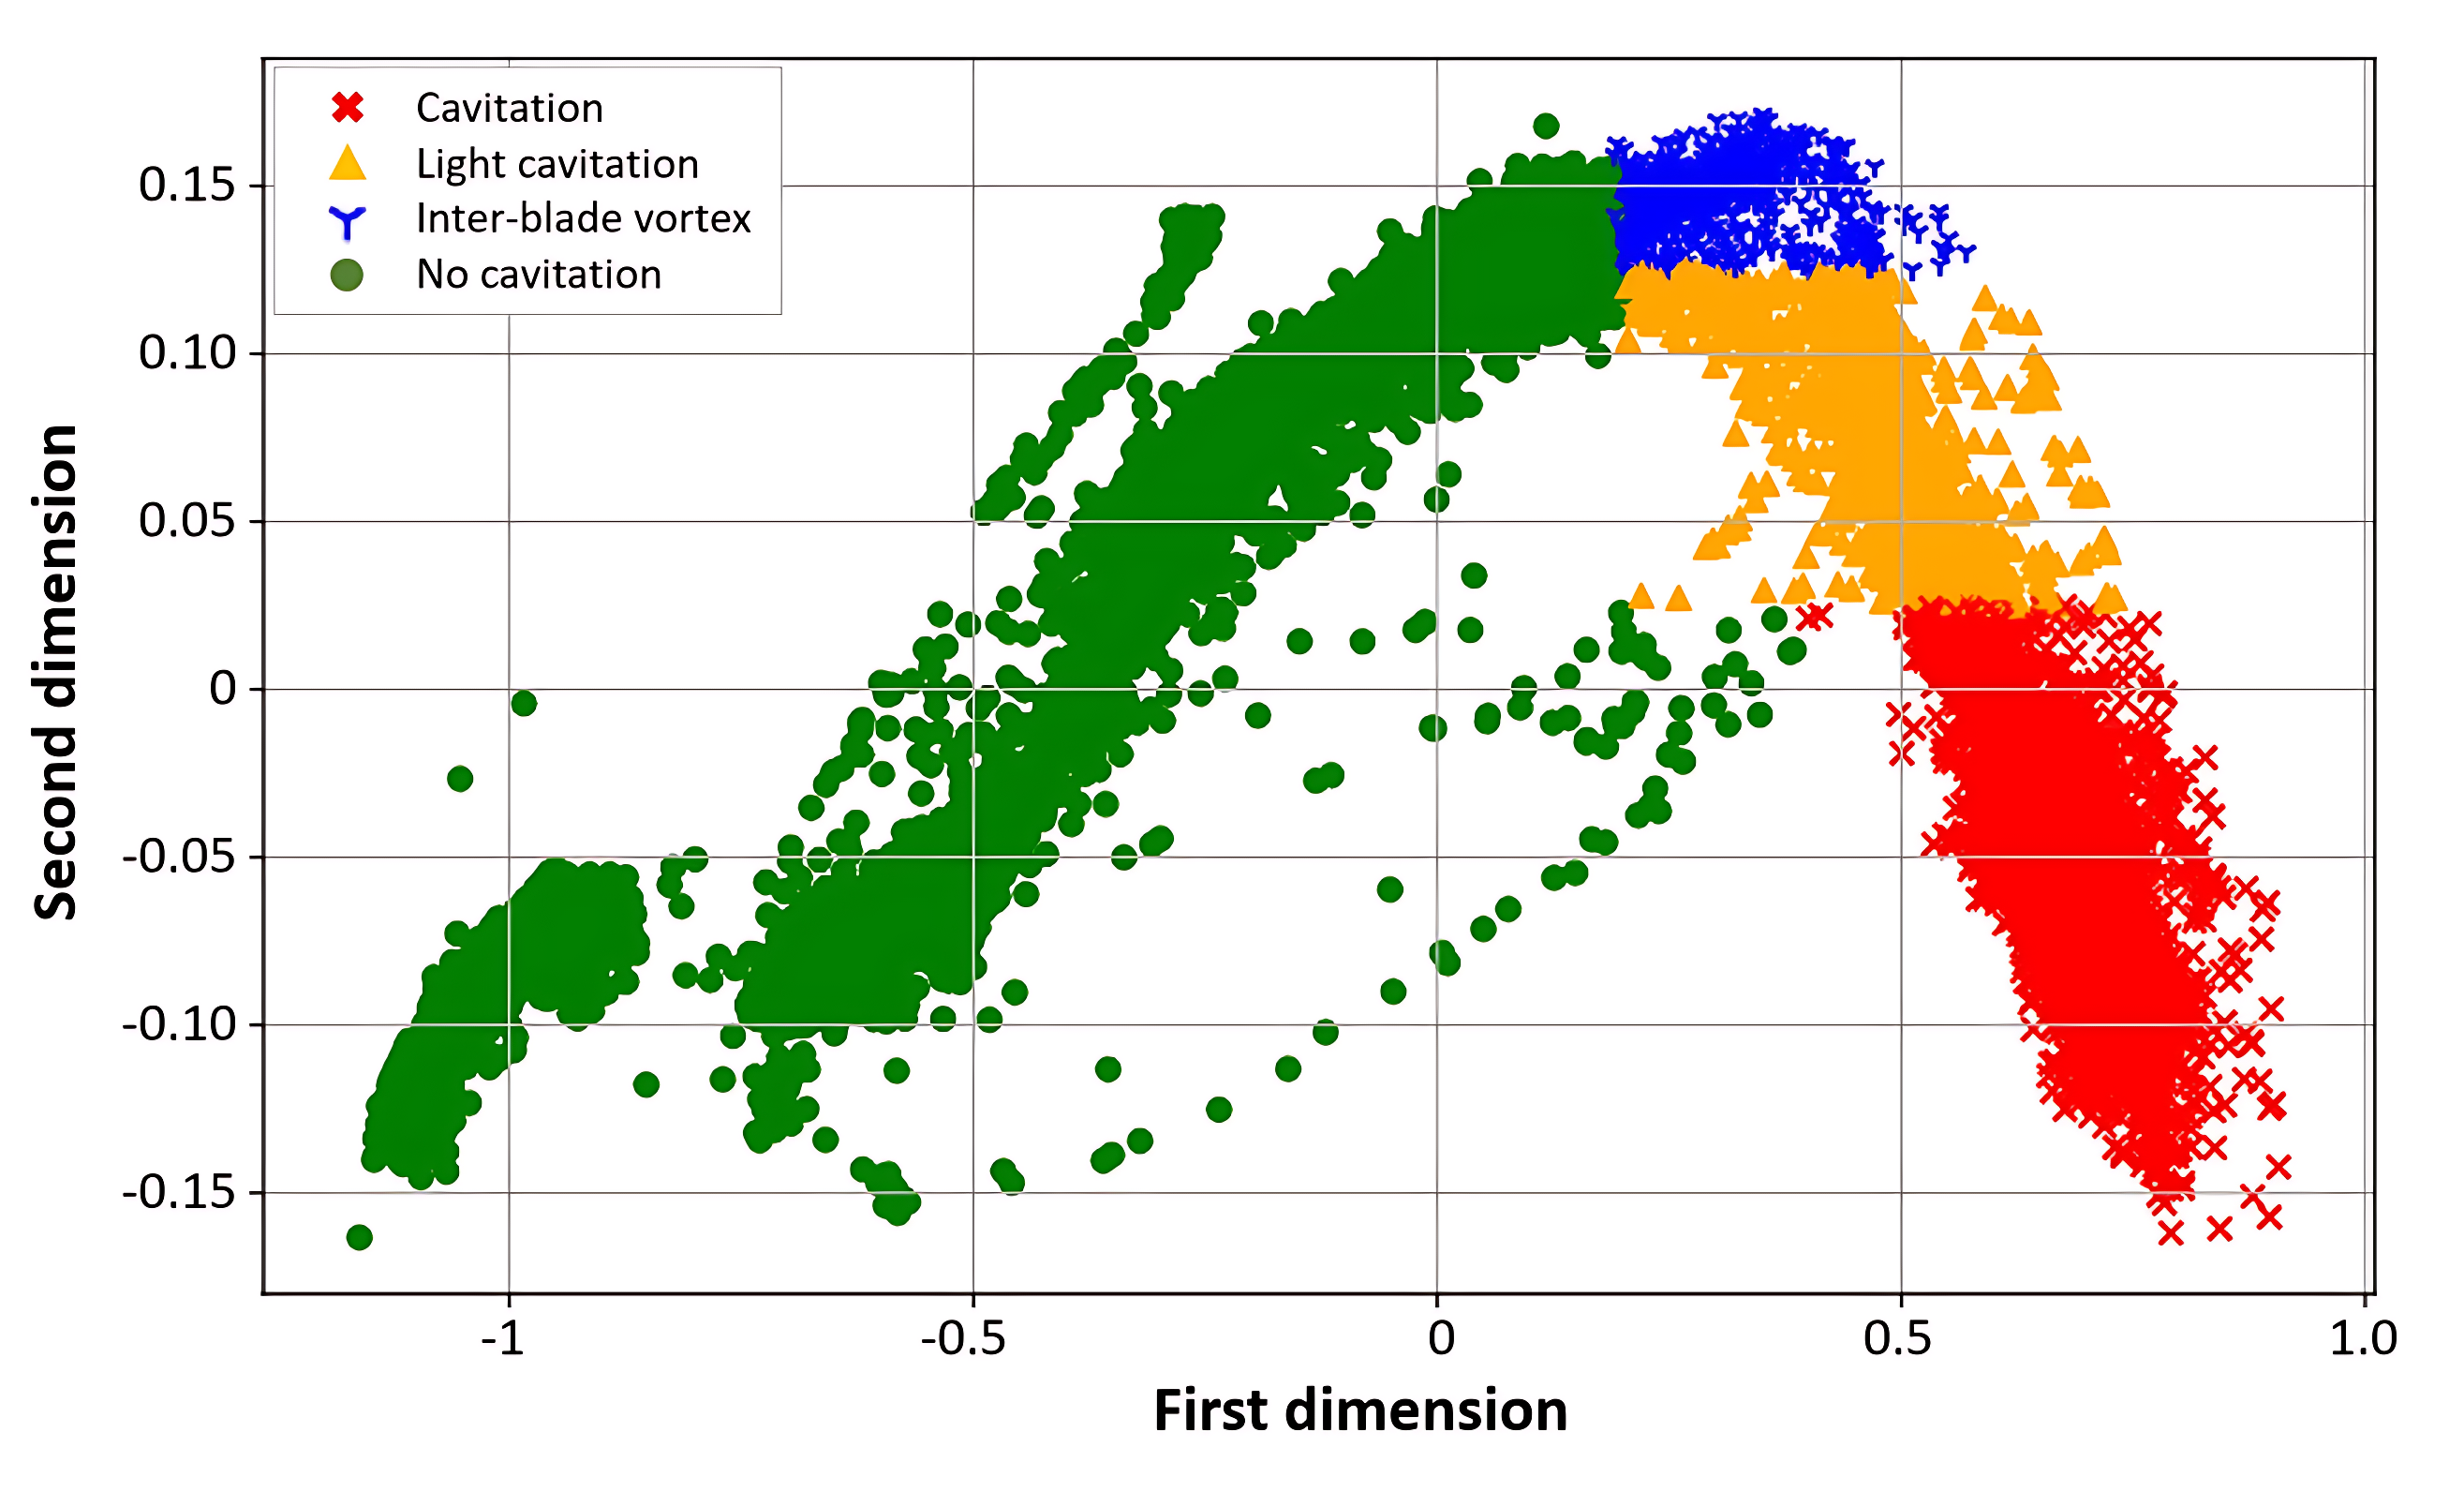
\includegraphics[width=.8\linewidth]{figs/Artigos/amini2022development/Figura6_Upscaler_2K.png}
    \caption{Projeção bidimensional dos dados de operação da turbina obtidos na usina de Ernen, classificando diferentes estados de escoamento: sem cavitação (verde), cavitação leve (amarelo), cavitação plena (vermelho) e vórtices interpalhetas (azul). Fonte: \citeonline{amini2022development}}
    \label{fig:amini2022developmentFig6}
\end{figure}
    
A Figura~\ref{fig:amini2022developmentFig6} exibe o resultado da classificação obtida no ambiente real da usina hidrelétrica. Cada ponto representa um vetor de características projetado em duas dimensões (via redução de dimensionalidade). Observa-se uma separação bem definida entre quatro condições: operação normal, cavitação leve, cavitação severa e presença de vórtices entre pás. Essa distinção confirma a robustez do modelo GMM, mesmo sob ruído operacional e variação de carga.

Em síntese, o estudo demonstra que a combinação entre processamento acústico e aprendizado de máquina é capaz de discriminar, com alta confiabilidade, diferentes estágios de cavitação tanto em condições laboratoriais quanto em ambiente industrial. Os resultados reforçam o potencial dessa abordagem para o monitoramento não intrusivo e o diagnóstico preditivo de turbinas hidráulicas.

Uma análise estatística complementar, realizada a partir do histórico operacional de sete anos da usina, revelou que as turbinas frequentemente operaram em faixas de carga parcial propensas à cavitação. Essa constatação sugere que o fenômeno pode ter contribuído para o desgaste prematuro de componentes e para a redução da eficiência global das máquinas, conforme apresentado na Figura~\ref{fig:amini2022developmentFig7}. Dessa forma, o sistema proposto pelos autores não apenas permite a detecção em tempo real, mas também possibilita o diagnóstico retrospectivo do número de horas em regime cavitante, ampliando seu potencial como ferramenta de manutenção preditiva.

\begin{figure}[H]
    \centering
    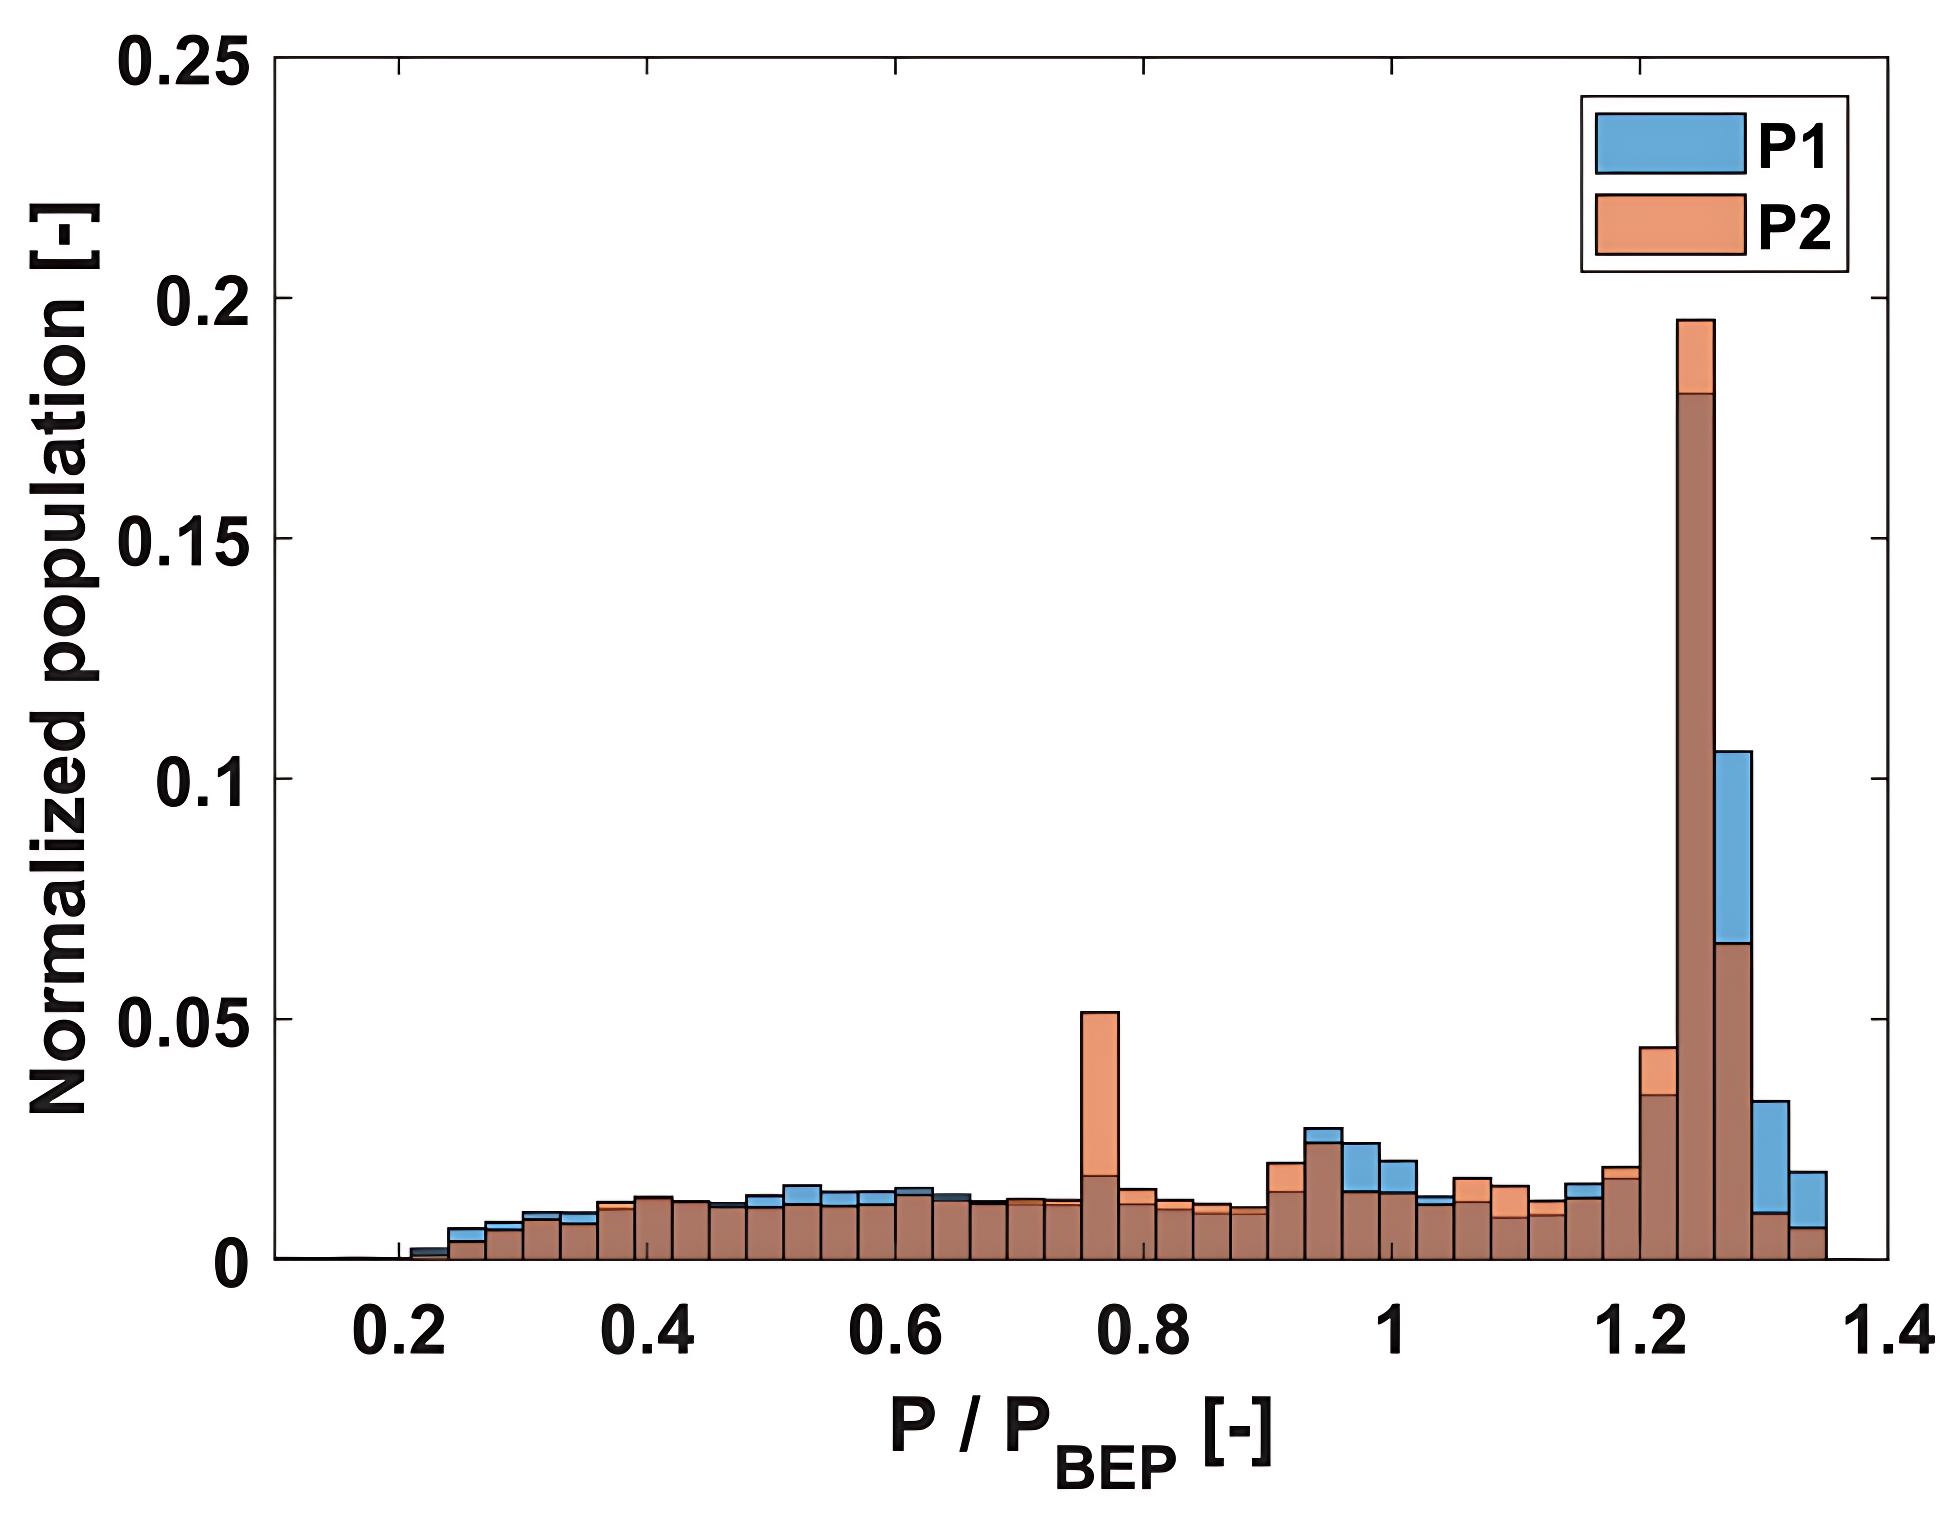
\includegraphics[width=.55\linewidth]{figs/Artigos/amini2022development/Figura7_Upscaler_2K.png}
    \caption{Distribuição normalizada da taxa de potência das duas turbinas idênticas (P1 e P2) da usina hidrelétrica de Ernen ao longo de um período de sete anos. Fonte: \citeonline{amini2022development}}
    \label{fig:amini2022developmentFig7}
\end{figure}

\linespread{1.28}\selectfont
A Figura~\ref{fig:amini2022developmentFig7} evidencia a frequência relativa de operação das duas turbinas, expressa em função da potência normalizada $P / P_{BEP}$, sendo $P_{BEP}$ a potência correspondente ao ponto de melhor eficiência \textit{Best Efficiency Point}. Observa-se que ambas as unidades operaram de forma recorrente acima de $1{,}2\,P_{BEP}$, faixa associada a maior risco de cavitação. Essa distribuição reforça a importância de sistemas de monitoramento contínuo, visto que períodos prolongados nesse regime podem causar erosão nas pás, vibrações excessivas e perdas de desempenho hidráulico. Além disso, a análise mostra a utilidade do sistema proposto não apenas para o acompanhamento em tempo real, mas também como ferramenta de avaliação histórica das condições operacionais e identificação de padrões de desgaste.

\linespread{1.28}\selectfont
Em conclusão, \citeonline{amini2022development} demonstram a viabilidade de um método não intrusivo para detecção de cavitação em turbinas hidráulicas, baseado em sinais acústicos e aprendizado de máquina. O sistema foi validado tanto em condições laboratoriais quanto em escala industrial, apresentando alta precisão na identificação de diferentes regimes de escoamento. Os autores ainda destacam o potencial de aprimoramento futuro por meio da incorporação de algoritmos mais avançados, capazes de distinguir entre diferentes tipos de cavitação e estimar índices de severidade. Tais avanços poderiam ser generalizados para outras configurações de turbinas mediante o uso de técnicas de aprendizado por transferência, ampliando o escopo de aplicação em sistemas hidrelétricos.

\linespread{1.28}\selectfont
A seguir, apresenta-se uma comparação sistemática dos principais tipos de sensores empregados na detecção de cavitação em bombas centrífugas, destacando suas faixas de frequência típicas, vantagens, limitações e aplicações mais adequadas. A Tabela \ref{tab:sensores_cavitacao} sintetiza essas características e proporciona ao leitor uma visão panorâmica dos trade-offs entre custo, sensibilidade e operacionalidade de cada sensor. Com isso, pretende-se facilitar a escolha adequada do sistema de medição conforme o estágio de cavitação, a criticidade do equipamento e o contexto de monitoramento industrial.

\begin{table}[H]
\footnotesize
\centering
\caption{Comparação entre diferentes tipos de sensores utilizados na detecção de cavitação em bombas centrífugas. Adaptado de \citeonline{liu2023review}.}
\label{tab:sensores_cavitacao}
\renewcommand{\arraystretch}{1.3}
\resizebox{\textwidth}{!}{%
\begin{tabular}{p{3.0cm} p{2.4cm} p{4.2cm} p{4.2cm} p{3.2cm}}
\hline
\textbf{Tipo de Sensor} & \textbf{Faixa típica de frequência} & \textbf{Vantagens principais} & \textbf{Limitações} & \textbf{Aplicações mais adequadas} \\ \hline

\textbf{Acelerômetro} &
1Hz – 20kHz &
Baixo custo, ampla disponibilidade e fácil instalação; fornece informações estruturais globais e permite análise conjunta de vibração e ruído. &
Menor sensibilidade para cavitação incipiente; fortemente influenciado por vibrações mecânicas externas e desbalanceamentos. &
Monitoramento geral da condição mecânica e detecção de cavitação moderada ou severa. \\ \hline

\textbf{Sensor de Emissão Acústica} &
100kHz – 1MHz &
Alta sensibilidade a eventos transientes e à cavitação incipiente; capaz de detectar impactos microscópicos e trincas. &
Custo mais elevado e necessidade de acoplamento adequado; suscetível à atenuação do sinal e à interferência estrutural. &
Detecção precoce de cavitação, fadiga e erosão em estágios iniciais. \\ \hline

\textbf{Sensor de Ruído} &
10Hz – 50kHz &
Instalação simples; útil para monitoramento de cavitação intensa e para análises comparativas entre regimes. &
Alta suscetibilidade a ruídos ambientais; dificuldade de calibração e isolamento de fontes. &
Testes experimentais, ensaios comparativos e diagnósticos de cavitação plena. \\ \hline

\textbf{Transdutor de Pressão} &
0 – 5kHz &
Mede diretamente variações de pressão e pulsação hidráulica; fornece informações sobre o escoamento e eficiência volumétrica. &
Baixa resolução temporal para eventos de curta duração; resposta limitada a altas frequências. &
Análise de instabilidades de escoamento, flutuações de pressão e correlação com regimes hidráulicos. \\ \hline
\end{tabular}}
\end{table}

\linespread{1.28}\selectfont
A Tabela \ref{tab:dominio_algoritmos} apresenta uma síntese dos principais “domínios de análise” e “algoritmos de classificação” empregados na detecção de cavitação em bombas centrífugas, conforme relatado por estudos recentes como \citeonline{liu2023review} e \citeonline{Zhang2015}. Esta comparação sistemática permite visualizar como diferentes tipos de sinais (vibração, emissão acústica, ruído, pulsação de pressão ou fusão de sensores) são processados em distintos domínios (tempo, frequência, tempo-frequência ou nível de atributos) e como tais sinais alimentam modelos de aprendizado de máquina ou redes neurais profundas (SVM, Random Forest, CNN, LSTM, entre outros). O conjunto de colunas “Técnicas de Extração de Atributos” e “Algoritmos / Modelos de Classificação” destaca os principais métodos em uso, enquanto a coluna “Referências Representativas” orienta o leitor para os estudos-chave que documentam cada abordagem. Em suma, esta tabela serve como ferramenta de orientação para a seleção de metodologias adequadas ao seu estudo — no qual a ênfase recai sobre o uso de dados de emissão acústica e a implementação simulada de uma CNN-1D — além de evidenciar a evolução do campo em direção a pipelines cada vez mais sofisticados e integrados.
\linespread{1.25}\selectfont
\begin{table}[H]
\footnotesize
\centering
\caption{Domínios de análise e algoritmos utilizados na detecção de cavitação com diferentes tipos de sinais. Fonte: O autor.}
\label{tab:dominio_algoritmos}
\renewcommand{\arraystretch}{1.3}
\resizebox{\textwidth}{!}{%
\begin{tabular}{p{3cm} p{2.9cm} p{4.5cm} p{4.2cm} p{2.8cm}}
\hline
\textbf{Tipo de Sinal} & \textbf{Domínio de Análise} & \textbf{Técnicas de Extração de Atributos} & \textbf{Algoritmos / Modelos de Classificação} & \textbf{Referências Representativas} \\ \hline

\textbf{Vibração} &
Tempo / Frequência &
RMS, curtose, fator de crista, frequência dominante, cepstrum, entropia espectral &
SVM, Random Forest, LSTM, CNN-1D &
\citeonline{liu2023review}, \citeonline{Wang2019} \\ \hline

\textbf{Emissão Acústica} &
Tempo / Frequência &
Amplitude, duração, invólucro retificado (MARSE), contagens, STFT, Wavelet Packet, espectrograma &
CNN-1D, CNN-2D (STFT), SAE, DBN &
\citeonline{liu2023review}, \citeonline{Zhang2015} \\ \hline

\textbf{Ruído} &
Tempo / Frequência &
Análise espectral, densidade de potência, centroides de frequência, coeficientes MFCC &
SVM, k-NN, CNN-2D, Transformer (Spectrogram) &
\citeonline{liu2023review}, \citeonline{Nurvitadhi2017} \\ \hline

\textbf{Pulsos de Pressão} &
Tempo / Frequência &
Média móvel, variância, análise de picos e modulações, componentes harmônicas &
Decision Tree, SVM, LSTM, HMM &
\citeonline{liu2023review} \\ \hline

\textbf{Multissensor} &
Tempo / Frequência / Feature-Level &
Concatenação de atributos normalizados, PCA, autoencoders, STFT sincronizada &
CNN híbrida, redes multimodais, aprendizado por transferência &
\citeonline{liu2023review}, \citeonline{Wang2019} \\ \hline
\end{tabular}}
\end{table}

% \textcolor{red}{Em processo de busca de trabalhos relacionados e leitura para depois escrever esta seção}


% Holford, K.M., et al. (2017). Acoustic emission for monitoring structural integrity: A review. Journal of Acoustic Emission.
% – Revisão clássica e bastante citada sobre princípios e aplicações de EA.

% Pollock, A.A. (2012). Acoustic Emission Inspection. NDT Handbook, ASNT.
% – Livro referência que explica fundamentos e aplicações práticas.

% Grosse, C. U., & Ohtsu, M. (2008). Acoustic Emission Testing. Springer.
% – Base teórica e metodológica, com aplicações em materiais e estruturas.

% Tang, J., et al. (2020). Acoustic emission-based condition monitoring and fault diagnosis of rotating machinery: A review. Applied Acoustics.
% – Excelente revisão ligando EA com análise em máquinas rotativas (seu caso).

% Revisões gerais de EA (Pollock, Holford, Grosse & Ohtsu).

% Aplicações em máquinas rotativas (Tang, Souza).

% Aplicações específicas em cavitação em bombas (Liu).
%\section{Aprendizado de Máquina}

Esta seção dedica-se à apresentação dos fundamentos conceituais e matemáticos do Aprendizado de Máquina, com ênfase nas abordagens supervisionadas e profundas aplicadas à análise de sinais. Inicialmente, discorrem-se os paradigmas de aprendizado, os principais algoritmos utilizados e suas respectivas áreas de aplicação. Em seguida, introduz-se o Aprendizado Profundo, e as Redes Neurais Multicamada Unidimensionais, destacando seu papel na extração automática de padrões complexos em sinais acústicos, como os gerados por fenômenos de cavitação e falhas incipientes em equipamentos rotativos.

A Inteligência Artificial constitui um campo interdisciplinar dedicado ao desenvolvimento de sistemas computacionais capazes de executar tarefas tradicionalmente associadas à cognição humana, tais como percepção, reconhecimento de padrões, tomada de decisão e raciocínio adaptativo. Seu objetivo central é reproduzir — e, em algumas situações, superar — aspectos do comportamento inteligente por meio de modelos matemáticos, estruturas algorítmicas e processamento de grandes volumes de dados.

Dentro desse panorama, o Aprendizado de Máquina representa uma subárea fundamental, responsável pelo estudo de algoritmos que aprendem a partir de exemplos. Em vez de depender de regras fixas programadas manualmente, esses algoritmos ajustam seus parâmetros internos de forma automática quando expostos a novos dados, aprimorando progressivamente seu desempenho em tarefas específicas. Essa característica torna o AM particularmente adequado a problemas complexos, não lineares ou de natureza estocástica, nos quais abordagens analíticas \mbox{tradicionais apresentam limitações.}

Entre os métodos mais influentes de Aprendizado de Máquina destacam-se as Redes Neurais Artificiais, inicialmente inspiradas em princípios do processamento neural biológico, desde o modelo formal de neurônio proposto por \citeonline{mcculloch1943logical} até as formulações consolidadas em obras clássicas como \citeonline{haykin2001redes}. Embora tais modelos tenham se tornado a base das arquiteturas modernas de aprendizado profundo, eles representam abstrações significativamente simplificadas do funcionamento do sistema nervoso real, empregando ativações contínuas e sincronizadas que não refletem diretamente a natureza pulsada e esparsa da comunicação neuronal biológica.

%Estudos recentes, como o de \citeonline{zheng2022introductory}, ampliam essa discussão ao comparar as Redes Neurais Artificiais convencionais (\textit{Artificial Neural Networks, ANNs}) com as Redes Neurais Pulsadas (\textit{Spiking Neural Networks, SNNs)}, modelos que buscam aproximar de forma mais fidedigna a dinâmica eletrofisiológica observada em neurônios reais. Enquanto as ANNs utilizam funções de ativação contínuas e densas, as SNNs operam com eventos discretos de disparo, \textit{spikes}, permitindo codificação temporal, maior esparsidade e potencial redução significativa no consumo energético. Além disso, diferem quanto aos mecanismos de aprendizagem: ao passo que as ANNs dependem tipicamente do \textit{backpropagation} e de gradientes contínuos, as SNNs investigam regras de aprendizado local inspiradas na biologia, como o \mbox{\textit{Spike-Timing-Dependent Plasticity, STDP.}}
%
%Assim, a literatura contemporânea evidencia uma evolução no entendimento da relação entre modelos computacionais e sistemas biológicos: as ANNs permanecem essenciais para aplicações práticas em larga escala devido à maturidade de suas técnicas de otimização, enquanto as SNNs representam uma fronteira promissora rumo a arquiteturas mais eficientes, esparsas e biologicamente plausíveis, conectando de modo mais direto os princípios da inteligência natural aos mecanismos da inteligência artificial.
%
%Nas redes naturais, cada neurônio, Figura \ref{fig:neuronio} é constituído por dendritos (responsáveis pela recepção dos estímulos provenientes de outras células), pelo corpo celular (que integra e processa os sinais recebidos) e pelo axônio (que transmite a saída para outras células). A comunicação ocorre por meio de impulsos elétricos, cuja frequência determina o nível de ativação do neurônio \citeonline{haykin2001redes}. Ainda que as redes biológicas não transmitam sinais negativos e apresentem organização morfológica extremamente heterogênea, constituem o modelo conceitual que fundamenta a criação das RNAs.
%
%\begin{figure}[H]
%	\centering
%	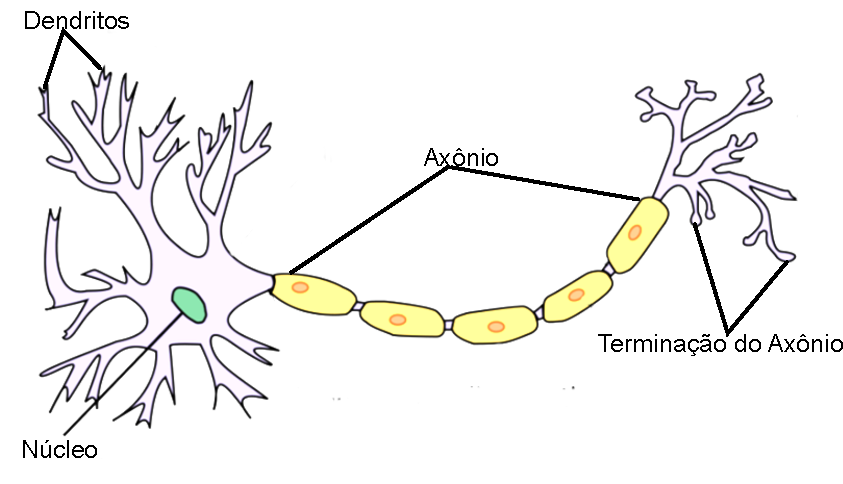
\includegraphics[width=0.65\linewidth]{figs/AprendizadoDeMaquina/Neuronio}
%	\caption{Ilustração de um Neurônio. Adaptado de \citeonline{zheng2022introductory}.}
%	\label{fig:neuronio}
%\end{figure}
%
%O neurônio artificial, por sua vez, é uma abstração computacional que captura os elementos essenciais do processo biológico:
%\begin{enumerate}[label=(\roman*)]
%	\item entradas provenientes do meio ou de outros neurônios;
%	\item sinapses simuladas por pesos, $w_1, w_2, w_3, ... w_n$ que modulam a influência de cada entrada;
%	\item um termo de viés (bias), que desloca a função de ativação e permite maior flexibilidade ao modelo;
%	\item um somador, responsável por combinar as entradas ponderadas;
%	\item uma função de ativação, que limita ou transforma a amplitude do sinal gerado; e
%	\item uma saída, transmitida à próxima camada da rede.
%\end{enumerate}
%
%Em conjunto, múltiplos neurônios artificiais organizados em camadas interconectadas formam arquiteturas capazes de aproximar funções complexas, detectar regularidades em dados ruidosos e extrair características relevantes de sinais multidimensionais. Essa capacidade emergente explica o amplo uso das RNAs em visão computacional, processamento de sinais, reconhecimento de fala, análise temporal e, particularmente neste trabalho, detecção de padrões em sinais de Emissão Acústica.
%
%\begin{figure}[H]
%	\centering
%	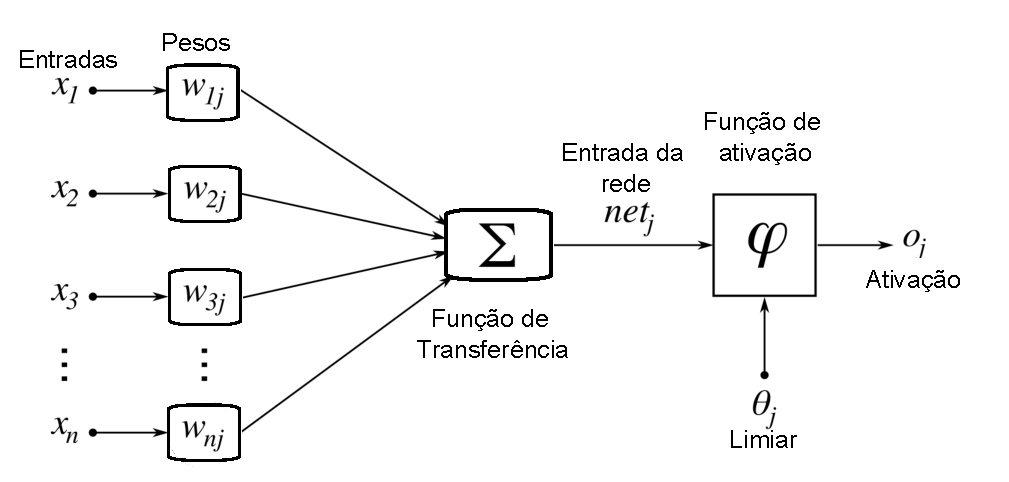
\includegraphics[width=0.85\linewidth]{figs/AprendizadoDeMaquina/NeuronioArtificial}
%	\caption{Neurônio artificial. Fonte: O autor.}
%	\label{fig:artificialneuronmodelenglish}
%\end{figure}
%
%O processo de aprendizado pode ocorrer de diferentes formas, dependendo da disponibilidade e do tipo de informação fornecida ao modelo. De modo geral, o ML é classificado em três categorias principais: aprendizado supervisionado, em que o modelo é treinado com exemplos rotulados; aprendizado não supervisionado, no qual se busca identificar padrões e agrupamentos ocultos em dados não rotulados; e aprendizado por reforço, baseado na interação contínua de um agente com um ambiente para maximizar recompensas acumuladas. Cada uma dessas abordagens apresenta características próprias e é adequada a contextos específicos de aplicação, como classificação, regressão, agrupamento e controle adaptativo.

Um subconjunto mais avançado e especializado do ML é o Aprendizado Profundo, que emprega arquiteturas compostas por múltiplas camadas de processamento, as chamadas redes neurais profundas. Essas estruturas são inspiradas no funcionamento do cérebro humano e são capazes de extrair representações hierárquicas e abstratas dos dados, capturando padrões complexos e não lineares. O DL tem se destacado em aplicações de alto impacto, como reconhecimento de voz e imagem, tradução automática, diagnóstico médico assistido e análise de sinais dinâmicos, devido à sua notável capacidade de generalização e robustez frente a grandes volumes de informação.

Nos últimos anos, a combinação entre aprendizado profundo e dispositivos de alto desempenho, como GPUs e FPGAs, tem ampliado significativamente o escopo de aplicação dessas técnicas, tornando viável a análise em tempo real de dados de alta taxa de amostragem — como os provenientes de sensores acústicos e vibrométricos empregados no monitoramento de máquinas rotativas. Essa integração entre IA e instrumentação digital representa um dos pilares do paradigma da manutenção preditiva inteligente, na qual modelos treinados são utilizados para detectar anomalias, prever falhas e otimizar a operação de sistemas industriais complexos.

%
%O campo do aprendizado de máquina abrange diferentes abordagens de treinamento, cada uma fundamentada na forma como o modelo interage com os dados e aprende a partir deles. De maneira geral, essas abordagens são organizadas em três grandes paradigmas: o aprendizado supervisionado, o aprendizado não supervisionado e o aprendizado por reforço. Cada paradigma apresenta características próprias, vantagens e limitações, sendo aplicável a diferentes tipos de problemas de modelagem, classificação e \mbox{controle em sistemas complexos.}

Os três paradigmas são sistematizados na Figura~\ref{fig:AprendizadoDeMaquinaConceitos}, que apresenta uma visão comparativa das principais estratégias de aprendizado e suas aplicações típicas em contextos industriais. Cada paradigma difere quanto à forma de aprendizado, à disponibilidade de rótulos nos dados e ao tipo de \textit{feedback} recebido durante o processo de treinamento.

\begin{figure}[H]
    \centering
    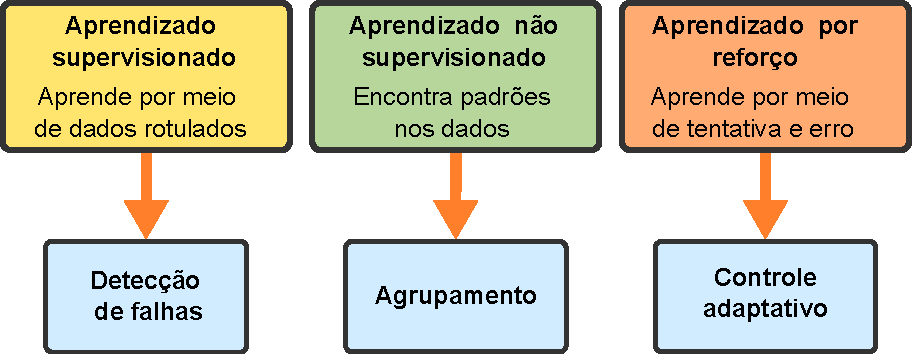
\includegraphics[width=0.7\linewidth]{figs/AprendizadoDeMaquina/AprendizadoDeMaquinaConceitos.pdf}
    \caption{Paradigmas do aprendizado de máquina e exemplos de aplicação industrial.\\Fonte: Em destaque o paradigma utilizado neste trabalha. O autor.}
    \label{fig:AprendizadoDeMaquinaConceitos}
\end{figure}

\begin{itemize}
    \item \textbf{Aprendizado Supervisionado:} Baseia-se na utilização de conjuntos de dados rotulados, nos quais cada amostra possui uma resposta conhecida. O modelo é treinado para aprender a relação entre entradas e saídas, generalizando o comportamento para novos dados. É amplamente empregado em tarefas de classificação e regressão, como a \textbf{detecção de falhas em sensores} ou a previsão de desgaste de componentes em bombas e turbinas.

    \item \textbf{Aprendizado Não Supervisionado:} Opera sobre dados não rotulados, buscando identificar padrões e estruturas ocultas. Utiliza técnicas como o \textit{k-means} ou análise de componentes principais (PCA) para agrupar dados semelhantes ou reduzir dimensionalidade. Essa abordagem é especialmente útil para \textbf{agrupamento de modos de operação}, detecção de anomalias e análise exploratória de sinais industriais.

    \item \textbf{Aprendizado por Reforço:} Difere dos paradigmas anteriores por envolver a interação contínua entre um agente e um ambiente. A cada ação, o agente recebe uma recompensa ou penalidade, aprendendo a maximizar seu desempenho ao longo do tempo. Esse método é aplicado em \textbf{controle adaptativo de processos industriais}, robótica e otimização de sistemas dinâmicos sob condições variáveis.
\end{itemize}

A Figura~\ref{fig:AprendizadoDeMaquinaConceitos} sintetiza graficamente essa classificação, destacando a complementaridade entre os paradigmas de Aprendizado Supervisionado, Não Supervisionado e por Reforço. Essa taxonomia ressalta a relevância das técnicas de \textit{Machine Learning} para a construção de sistemas inteligentes que não apenas identificam falhas, mas extraem conhecimento útil para otimizar processos. Em última análise, o diagrama ilustra o arcabouço conceitual para o desenvolvimento de soluções voltadas à manutenção preditiva, à análise de falhas em componentes mecânicos e ao monitoramento em  com baixa latência de inferência, promovendo a detecção precoce de anomalias e garantindo a maior robustez de decisão no ambiente industrial.

%O aprendizado de máquina engloba uma ampla variedade de algoritmos, cada um com princípios matemáticos e áreas de aplicação específicas. A escolha do modelo mais adequado depende diretamente da natureza dos dados, do objetivo da análise e das restrições computacionais do sistema. De forma geral, entre os principais algoritmos utilizados em ML, são:
%
% \begin{itemize}
%     \item \textbf{Redes Neurais Artificiais (ANNs):} inspiradas no funcionamento biológico do cérebro, compostas por camadas de neurônios interconectados capazes de aprender relações complexas entre variáveis.
%     \item \textbf{Árvores de Decisão e Random Forest:} modelos baseados em regras hierárquicas que realizam divisões sucessivas do espaço de dados, amplamente empregados em classificação e regressão devido à sua interpretabilidade.
%     \item \textbf{Máquinas de Vetores de Suporte (SVMs):} algoritmos que buscam maximizar a margem entre classes, eficazes em conjuntos de dados de alta dimensionalidade e com fronteiras não lineares.
%     \item \textbf{Modelos de Mistura Gaussiana (GMMs):} utilizados para modelar distribuições probabilísticas complexas e realizar agrupamento (clustering) de dados de natureza heterogênea.
%     \item \textbf{Métodos de Ensemble, como Gradient Boosting:} combinam múltiplos modelos fracos (geralmente árvores de decisão) para formar um modelo forte, otimizando o desempenho preditivo e reduzindo o erro de generalização.
%     \item \textbf{Redes Neurais Multicamada (MLP):} arquiteturas profundas projetadas para extrair automaticamente padrões espaciais ou temporais, amplamente empregadas em visão computacional, processamento de áudio e diagnóstico industrial.
% \end{itemize}

%\begin{table}[H]
%\centering
%\caption{Principais algoritmos de aprendizado de máquina e suas características gerais.}
%\label{tab:algoritmos_ml}
%\renewcommand{\arraystretch}{1.3}
%\resizebox{\textwidth}{!}{%
%\begin{tabular}{p{4cm} p{11cm}}
%\hline
%\textbf{Algoritmo} & \textbf{Descrição Geral} \\ \hline
%
%\textbf{Redes Neurais Artificiais (ANNs)} &
%Inspiradas no funcionamento biológico do cérebro, são compostas por camadas de neurônios interconectados capazes de aprender relações complexas entre variáveis, sendo adequadas para modelar fenômenos não lineares. \\ \hline
%
%\textbf{Árvores de Decisão e Random Forest} &
%Modelos baseados em regras hierárquicas que realizam divisões sucessivas do espaço de dados. São amplamente empregados em tarefas de classificação e regressão, destacando-se pela interpretabilidade e robustez a ruído. \\ \hline
%
%\textbf{Máquinas de Vetores de Suporte (SVMs)} &
%Algoritmos que buscam maximizar a margem entre classes, sendo eficazes em conjuntos de dados de alta dimensionalidade e com fronteiras não lineares, especialmente em classificações binárias. \\ \hline
%
%\textbf{Modelos de Mistura Gaussiana (GMMs)} &
%Utilizados para modelar distribuições probabilísticas complexas, permitindo identificar grupos latentes de dados (\textit{clustering}) em aplicações de natureza heterogênea e não supervisionada. \\ \hline
%
%\textbf{Métodos de Ensemble (ex.: Gradient Boosting)} &
%Combinam múltiplos modelos fracos (geralmente árvores de decisão) para formar um modelo mais robusto, otimizando o desempenho preditivo e reduzindo o erro de generalização. \\ \hline
%
%\textbf{Redes Neurais Multicamada (MLP)} &
%Arquiteturas profundas projetadas para extrair automaticamente padrões espaciais ou temporais por meio de filtros convolucionais, amplamente aplicadas em visão computacional, processamento de sinais acústicos e diagnóstico industrial. \\ \hline
%\end{tabular}}
%\end{table}
%
%Entre esses métodos, as \textbf{Redes Neurais Multicamada (MLP)} merecem destaque por sua capacidade de extrair representações hierárquicas de dados brutos, reduzindo a necessidade de pré-processamento manual. Embora originalmente concebidas para o reconhecimento de imagens, as MLP têm-se mostrado extremamente eficazes na análise de sinais acústicos e séries temporais, como os provenientes de sensores de emissão acústica, devido à sua habilidade em capturar correlações locais \mbox{e padrões de alta frequência.}
%
%A arquitetura típica de uma CNN é composta por diferentes tipos de camadas, cada uma com função específica no processo de aprendizado:
%
%\begin{itemize}
%    \item \textbf{Camadas Multicamada:} realizam a operação de convolução, extraindo padrões locais (por exemplo, bordas em imagens ou picos em sinais de emissão acústica).
%    \item \textbf{Camadas de Pooling:} reduzem a dimensionalidade dos mapas de ativação, preservando as informações mais relevantes e diminuindo o custo computacional.
%    \item \textbf{Camadas Totalmente Conectadas (Fully Connected):} integram as características extraídas nas etapas anteriores para a tomada de decisão final, como a classificação do tipo de falha.
%    \item \textbf{Funções de Ativação (ex., ReLU, sigmoid, softmax):} introduzem não linearidade ao modelo, permitindo capturar relações complexas entre as variáveis e melhorar a capacidade de generalização.
%\end{itemize}
%
%Esses elementos, combinados em múltiplos níveis, formam uma estrutura profunda e adaptável, capaz de aprender automaticamente as representações mais relevantes dos dados — característica essencial para aplicações em manutenção preditiva, diagnóstico de falhas e monitoramento inteligente de sistemas industriais.

\section{Redes Neurais MLP)}

\textcolor{red}{Estou Escrevendo}

%A literatura recente tem demonstrado um crescimento expressivo no interesse por métodos de aprendizado profundo, com diversas arquiteturas, como Redes Neurais Profundas (\textit{Deep Neural Network, DNNs}), Redes de Crença Profunda (\textit{Deep Belief Networks, DBNs}), Redes Neurais Recorrentes (\textit{Recurrent Neural Networks, RNN}), Redes Neurais Multicamada (\textit{Convolutional Neural Networks, MLP}) e Transformers, aplicadas a domínios variados, incluindo visão computacional, reconhecimento de fala, processamento de linguagem natural, bioinformática, análise de imagens médicas, ciências climáticas, inspeção de materiais e outras áreas emergentes. Conforme discutido por \citeonline{cacciari2024hands}, embora múltiplas arquiteturas tenham sido propostas para lidar com problemas unidimensionais, as MLP de uma dimensão, continuam sendo amplamente utilizadas e ainda aparecem com maior frequência na literatura indexada entre 2018 e 2023 do que alternativas mais recentes.
%
%O uso de rede MLP permanece menos difundido quando comparado a CNN-2D e CNN-3D, refletindo uma lacuna de pesquisa que inclui tanto menor volume de publicações quanto menor quantidade de revisões sistemáticas dedicadas exclusivamente ao tema. Ainda assim, \citeonline{cacciari2024hands} destacam que as rede MLP constituem uma tecnologia particularmente adequada para aplicações em tempo real, em virtude de sua menor complexidade computacional e capacidade de lidar diretamente com sinais brutos. Exemplos incluem detecção em espectroscopia Raman, linearização de amplificadores em sistemas 5G, monitoramento de interferência eletromagnética em sistemas de potência, classificação de sinais acústicos cardíacos, análise de áudio ambiental, \mbox{modelagem de fala e classificação de música.}
%
%As Redes Neurais Multicamada Unidimensionais representam uma extensão natural das MLP originalmente aplicadas a imagens, adaptadas para o processamento de sinais temporais. Diferentemente das MLP bidimensionais, nas quais os filtros convolucionais percorrem duas dimensões espaciais (altura e largura da imagem), as rede MLP operam exclusivamente sobre a dimensão temporal dos dados, tornando-as especialmente adequadas para o tratamento de séries temporais, \mbox{vibrações e sinais de emissão acústica (EA)}.
%
%\subsection{Fundamentos da Convolução Unidimensional e Análise Comparativa}
%
%As Redes Neurais Multicamada, embora popularizadas pelo sucesso massivo em tarefas de visão computacional, possuem uma formulação matemática generalizável para dados de diferentes dimensionalidades. Conforme discutido por \citeonline{kiranyaz20211d}, enquanto as CNN-2D se tornaram o padrão de fato para processamento de imagens, a adaptação dessa arquitetura para sinais unidimensionais oferece vantagens estruturais decisivas para o processamento de séries temporais, especialmente em cenários com restrições de hardware e latência.
%
%A operação fundamental de uma rede MLP assemelha-se à filtragem digital clássica (FIR), porém com a distinção crucial de que os coeficientes do filtro (pesos do \textit{kernel}) são parâmetros aprendidos através do algoritmo de \textit{Backpropagation}.
%
%Matematicamente, considere um sinal de entrada $x \in \mathbb{R}^{N}$ e um filtro (kernel) $w \in \mathbb{R}^{K}$, onde $K$ representa o tamanho do kernel (campo receptivo local). A convolução linear direta, \textit{valid padding},  para a $k$-ésima camada e o $j$-ésimo neurônio resulta em um mapa de ativação $y$, definido por \ref{eq:conv1d}:
%
%\begin{equation}
%	y_j[i] = f\left( b_j + \sum_{m=1}^{K} w_j[m] \cdot x[i + m - 1] \right)
%	\label{eq:conv1d}
%\end{equation}
%
%\noindent em que:
%
%\begin{itemize}
%	\item $b_j$ é o viés (\textit{bias}) do $j$-ésimo neurônio;
%	\item $f(\cdot)$ é a função de ativação não linear (tipicamente ReLU, Leaky ReLU ou TanH);
%	\item $i$ denota o índice temporal da sequência de saída.
%\end{itemize}
%
%Diferentemente da convolução 2D, que exige varredura em eixos horizontal e vertical, a operação em Eq. \ref{eq:conv1d} ocorre estritamente ao longo do eixo temporal. Segundo \citeonline{kiranyaz20211d}, essa redução de dimensionalidade implica que tanto a \textit{Forward Propagation} quanto a \textit{Backpropagation} podem ser implementadas como operações vetoriais simples, em oposição às operações matriciais complexas exigidas pelas MLP-2D.
%
%
%Para fins de implementação computacional e futura síntese em hardware, o procedimento de inferência de uma única camada MLP pode ser descrito estruturalmente pelo Algoritmo \ref{alg:conv1d_fwd}.
%
%\begin{algorithm}[H]
%	\caption{Processo de Inferência de uma Camada Convolucional 1D (Forward Propagation)}
%	\label{alg:conv1d_fwd}
%	\begin{algorithmic}[1]
%		\Require Vetor de entrada $x$ de tamanho $N$
%		\Require Kernel (filtro) $w$ de tamanho $K$
%		\Require Viés $b$
%		\Require Função de ativação $f(\cdot)$
%		\Require Passo de deslocamento (\textit{stride}) $S$
%		\Ensure Mapa de características de saída $y$
%		
%		\State $L_{out} \gets \lfloor (N - K)/S \rfloor + 1$ \Comment{Calcula dimensão da saída}
%		\State Inicializar vetor $y$ com zeros de tamanho $L_{out}$
%		
%		\For{$i \gets 0$ \textbf{to} $L_{out} - 1$} \Comment{Loop sobre a posição da janela}
%		\State $soma \gets 0$
%		\For{$k \gets 0$ \textbf{to} $K - 1$} \Comment{Loop sobre o kernel (MAC)}
%		\State $soma \gets soma + w[k] \times x[i \cdot S + k]$
%		\EndFor
%		\State $y[i] \gets f(soma + b)$ \Comment{Aplica viés e não-linearidade}
%		\EndFor
%		
%		\State \Return $y$
%	\end{algorithmic}
%\end{algorithm}
%
%A análise do Algoritmo \ref{alg:conv1d_fwd} evidencia a natureza sequencial e determinística da operação. Os laços aninhados (linhas 3 e 5) representam a operação de \textit{Multiply-Accumulate}, MAC, que é o bloco fundamental de processamento em DSPs e FPGAs. Note-se que, em uma implementação de hardware paralela, o laço interno (linhas 5-7) pode ser desenrolado (\textit{unrolled}), permitindo que todas as multiplicações do kernel ocorram em um único ciclo de \textit{clock}, característica explorada para atingir baixa latência.
%
%A topologia de uma rede MLP típica, conforme proposta por \citeonline{kiranyaz20211d}, divide-se em dois blocos funcionais principais:
%
%\begin{enumerate}
%	\item \textbf{Extração de Características (\textit{Feature Extraction}):} Composta por camadas alternadas de convolução 1D e subamostragem (\textit{pooling}). Nesta etapa, a rede aprende a identificar padrões morfológicos no sinal, como picos, oscilações transientes e variações de frequência, gerando tensores de baixa dimensão que resumem o conteúdo informacional da entrada.
%	\item \textbf{Classificação \textit{(MLP Backend}):} Os mapas de características resultantes são achatados (\textit{flattened}) ou processados via \textit{Global Average Pooling} para alimentar camadas densas, \textit{Fully Connected}, que realizam o mapeamento final para as classes de interesse (ex: ``Normal'' vs. ``Cavitação'').
%\end{enumerate}
%
%Uma vantagem arquitetural apontada por \citeonline{kiranyaz20211d} é a capacidade das MLP-1D de atingirem alta performance com arquiteturas ``rasas'' (\textit{shallow architectures}), frequentemente com apenas duas ou três camadas convolucionais ocultas. Isso contrasta com modelos de visão computacional (como ResNet ou VGG), que demandam dezenas de camadas para capturar hierarquias espaciais complexas.
%
%A distinção entre as abordagens não é apenas uma questão de formato de entrada, mas de eficiência computacional e adequação ao domínio do problema. Em aplicações de monitoramento de máquinas, a prática comum de converter sinais 1D em imagens 2D (via Espectrogramas ou Transformada \textit{Wavelet}) para utilizar as CNN-2D pré-treinadas introduz redundância e custo computacional desnecessário.A Tabela \ref{tab:comp_cnn} sumariza as diferenças estruturais destacadas na literatura.
%
%\begin{table}[H]
%	\centering
%	\footnotesize
%	\caption{Comparativo estrutural entre rede MLP e CNN-2D. Adaptado de \citeonline{kiranyaz20211d}.}
%	\label{tab:comp_cnn}
%	\resizebox{\textwidth}{!}{
%	\begin{tabular}{lll}
%		\toprule
%		\textbf{Critério} & \textbf{rede MLP} & \textbf{CNN-2D} \\
%		\midrule 
%		\textbf{Natureza da Entrada} & Vetor ou Série Temporal & Matriz (Imagem, Espectrograma) \\
%		\textbf{Movimento do Kernel} & Unidimensional (apenas tempo) & Bidimensional (altura e largura) \\
%		\textbf{Complexidade Computacional} & $O(N_k \cdot L)$ & $O(N_k \cdot H \cdot W)$ \\ \textbf{Parâmetros Treináveis} & Baixo (kernels vetoriais) & Alto (kernels matriciais)\\
%		\textbf{Requisito de Hardware} & Baixo (viável em CPU/FPGA simples) & Alto (geralmente requer GPU) \\
%		\textbf{Profundidade da Rede} & Tipicamente Rasa (Compacta) & Profunda\\ \textbf{Tratamento de Dados} & Processa sinal bruto (\textit{raw data}) & Exige conversão tempo-frequência \\
%		\bottomrule
%	\end{tabular}}
%\end{table}
%
%A escolha pela rede MLP neste trabalho é fundamentada nas propriedades de ``Compacidade'' e ``Eficiência Adaptativa'' definidas por \citeonline{kiranyaz20211d}.Primeiramente, a convolução 1D preserva a topologia temporal original do sinal de Emissão Acústica, permitindo que a rede explore correlações de fase e eventos transientes que poderiam ser suavizados ou perdidos em uma conversão para espectrograma.Em segundo lugar, a redução drástica no número de Operações de Multiplicação e Acumulação, MACs, torna a rede MLP inerentemente adequada para implementação em FPGA. Enquanto uma CNN-2D exigiria \textit{buffers} de linha complexos e intenso acesso à memória externa para armazenar mapas bidimensionais intermediários, a rede MLP permite um fluxo de dados simplificado e menor latência de inferência, requisitos mandatórios para o sistema de monitoramento em tempo real proposto.

%\section{Field-Programmable Gate Arrays (FPGAs)}

Nesta seção, discutem-se os princípios de funcionamento, a arquitetura e o fluxo de desenvolvimento de sistemas baseados em Field-Programmable Gate Arrays (FPGAs), dispositivos semicondutores programáveis amplamente utilizados em aplicações de processamento digital em tempo real. São abordadas as principais estruturas internas — como blocos lógicos configuráveis, memórias internas e blocos de DSP, e as vantagens oferecidas por esse tipo de hardware em termos de paralelismo, reconfigurabilidade e eficiência energética. Por fim, destaca-se o potencial dos FPGAs como plataforma para a implementação de algoritmos de aprendizado de máquina embarcados, consolidando seu papel em sistemas inteligentes de monitoramento e diagnóstico industrial.

Os FPGAs são dispositivos semicondutores programáveis que permitem a reconfiguração de sua lógica interna mesmo após a fabricação. Essa característica os diferencia dos \textit{Application-Specific Integrated Circuits} (ASICs), projetados para executar uma única função fixa e imutável. Nos FPGAs, o comportamento do hardware é definido por meio de uma descrição de hardware (\textit{Hardware Description Language},HDL), como VHDL ou Verilog, que é sintetizada em uma matriz de blocos lógicos interconectáveis, possibilitando a criação de circuitos digitais personalizados.

A principal vantagem dessa arquitetura reside na \textbf{reconfigurabilidade}, que permite alterar ou atualizar a funcionalidade do sistema sem modificar o hardware físico. Essa flexibilidade torna os FPGAs especialmente atrativos para prototipagem rápida, validação de novas arquiteturas digitais e desenvolvimento de sistemas embarcados adaptáveis. Além disso, os FPGAs combinam desempenho próximo ao de soluções ASIC com o benefício de um tempo de desenvolvimento significativamente menor. Entre as vantagens mais relevantes, destacam-se:

\begin{itemize}
    \item \textbf{Flexibilidade e reconfigurabilidade pós-produção:} possibilitam ajustes no hardware conforme mudanças de requisitos ou algoritmos;
    \item \textbf{Prototipagem rápida:} permitem testar novas arquiteturas digitais sem necessidade de fabricação de chips dedicados;
    \item \textbf{Adaptação dinâmica:} possibilitam o reuso do mesmo hardware em diferentes aplicações por meio de reprogramação parcial;
	\item \textbf{Alto desempenho e paralelismo:} capazes de executar múltiplas operações simultaneamente, com baixa latência, sendo ideais para aplicações como processamento de sinais, visão computacional, telecomunicações e inferência eficiente de redes neurais.
\end{itemize}

Apesar das vantagens, o uso de FPGAs também apresenta desafios significativos. O desenvolvimento demanda conhecimento especializado em eletrônica digital, linguagens HDL e ferramentas de síntese e roteamento, resultando em uma curva de aprendizado acentuada. Além disso, há limitações intrínsecas relacionadas ao número de blocos lógicos disponíveis, à quantidade de memória interna (BRAM) e ao consumo energético, que pode superar o de soluções ASIC quando operando continuamente.

Nos últimos anos, o avanço das aplicações em Inteligência Artificial e Aprendizado Profundo  impulsionou o uso de FPGAs como plataformas de aceleração computacional. Diferentemente das GPUs, que oferecem paralelismo massivo mas com arquitetura fixa, os FPGAs permitem customizar o fluxo de dados e a precisão dos cálculos, adequando-se ao modelo neural e às restrições de desempenho e energia. Esse fator é particularmente relevante em aplicações de inferência em tempo real, onde o equilíbrio entre latência, \textit{throughput} e consumo energético é crítico.

Um dos avanços mais importantes nessa área é a utilização de técnicas de \textbf{quantização de redes neurais}, que reduzem a precisão numérica dos pesos e ativações (por exemplo, de 32 bits para 8 ou 4 bits), mantendo desempenho próximo ao original e reduzindo drasticamente o custo computacional. Essa abordagem viabiliza a implementação de modelos complexos em hardware reconfigurável, preservando acurácia e eficiência.

Dessa forma, os FPGAs consolidam-se como uma plataforma versátil para aplicações em IA embarcada e processamento de sinais industriais, oferecendo uma solução intermediária entre a flexibilidade dos processadores convencionais e a \mbox{eficiência dos ASICs dedicados.}

Compreendidos os princípios gerais de funcionamento e as motivações que tornam os FPGAs atraentes para aplicações de processamento paralelo e aprendizado de máquina embarcado, torna-se relevante examinar sua estrutura interna com maior detalhe. A compreensão dos blocos constituintes e de suas interconexões é essencial para o correto aproveitamento dos recursos de hardware disponíveis e para o desenvolvimento de arquiteturas otimizadas em termos de desempenho, latência e consumo energético.  

Na subseção a seguir, é apresentada a arquitetura interna de um FPGA moderno, destacando-se seus principais componentes, como blocos lógicos configuráveis, memórias internas, blocos DSP e transceptores seriais, e a forma como esses elementos interagem para viabilizar a implementação de circuitos digitais complexos \mbox{em um ambiente reconfigurável.}

\subsection*{Arquitetura Interna de um FPGA}

O desempenho e a flexibilidade dos FPGAs decorrem diretamente de sua arquitetura interna, representada da Figura~\ref{fig:FPGA_internal_architeture}, projetada para combinar \textit{lógica reconfigurável}, \textit{interconexões programáveis} e \textit{blocos especializados} em um mesmo dispositivo. Essa estrutura hierárquica permite que diferentes funções digitais sejam implementadas em paralelo, de acordo com as necessidades do projeto, tornando o FPGA uma plataforma versátil para aplicações de alta complexidade \citeonline{langhammer2014design}.

\begin{figure}[H]
    \centering
    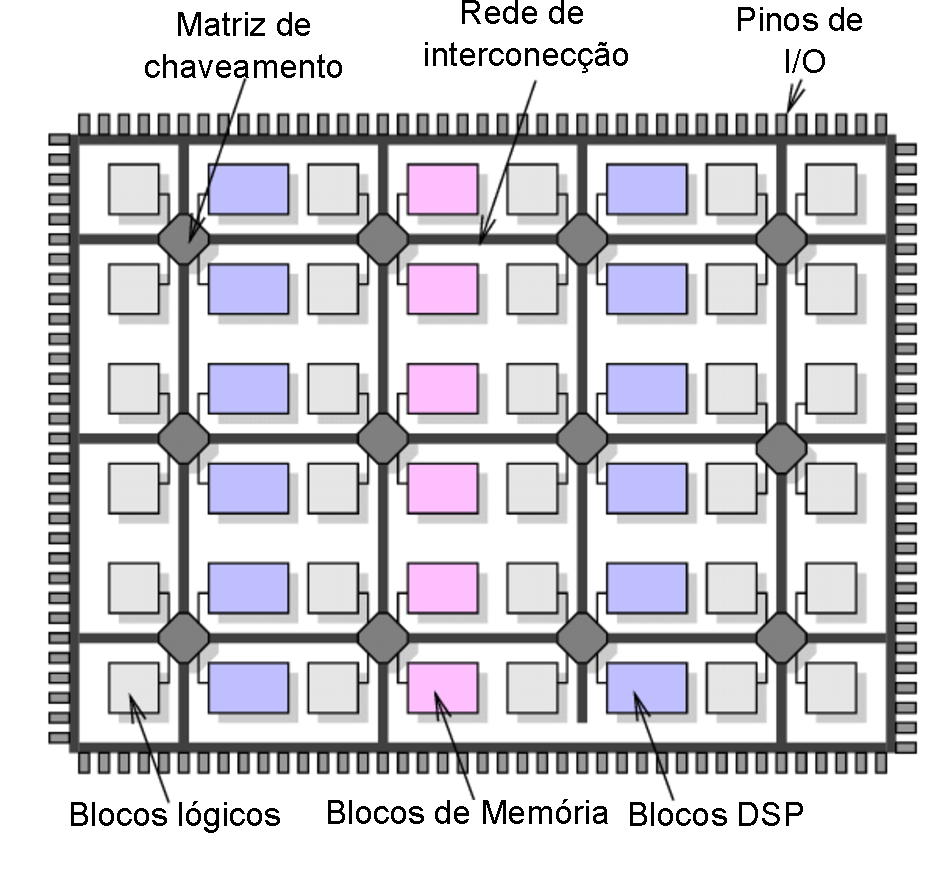
\includegraphics[width=0.65\linewidth]{figs/FPGA/FPGA.pdf}
    \caption{Arquitetura interna de um FPGA. Adaptado de \citeonline{langhammer2014design}}
    \label{fig:FPGA_internal_architeture}
\end{figure}

De modo geral, a arquitetura de um FPGA moderno pode ser compreendida como um arranjo matricial de elementos lógicos, conectados por uma rede de roteamento programável e complementados por blocos dedicados de memória, processamento aritmético e comunicação Figura~\ref{fig:FPGA_internal_architeture}. Essa organização possibilita a construção de circuitos personalizados, capazes de operar de forma determinística e com latência previsível — características essenciais em sistemas embarcados e aplicações de tempo real.

Os principais componentes que compõem essa arquitetura, enfatizando suas funções e a forma como interagem na implementação de sistemas digitais \mbox{complexos são listado a seguir:}

\begin{itemize}
	\item \textbf{Blocos Lógicos Configuráveis (CLBs / Logic Elements)}
	Cada bloco lógico geralmente contém uma \textit{Look-Up Table, LU)}, \textit{flip-flops} (registradores) e lógica de seleção (multiplexadores). As LUTs são usadas para implementar funções lógicas arbitrárias (até uma certa \textit{fan-in}). Os \textit{flip-flops} armazenam estado, e a lógica de interconexão dentro do bloco permite configuração de lógica combinacional ou sequencial.
	
	\item \textbf{Rede de Interconexão Programável}
	Os blocos lógicos são conectados por uma malha (ou rede) de trilhas metálicas (vias, linhas horizontais e verticais) e \textit{switches} programáveis (\textit{crossbars}, multiplexadores, \textit{buffers}). Essa rede determina como os sinais trafegam entre blocos. O desafio de roteamento (satisfazer todas as conexões com restrições de temporização\textit{timing}) é crítico para o desempenho final.
	
	\item \textbf{Blocos de Entrada/Saída (I/O Blocks)}
	Permitem a interface com sinais externos (barramentos, memórias externas, sensores, periféricos). Tipicamente suportam múltiplos padrões de tensão e protocolos (por exemplo, LVDS, PCIe, DDR, \mbox{interfaces de alta velocidade).}
	
	\item \textbf{Blocos de Memória (BRAM / Block RAM)}
	Memórias internas, distribuídas dentro do FPGA, oferecem armazenamento rápido e local para dados intermediários, buffers, tabelas etc. São mais rápidas e eficientes que acessar memória externa.
	
	\item \textbf{Blocos DSP (DSP Slices)}
	Otimizados para operações aritméticas, especialmente multiplicações, multiplicações acumuladas e outras operações de ponto fixo ou ponto flutuante limitada. Permitem acelerar operações pesadas tipicamente usadas em filtros, transformadas, redes neurais etc.
	
	\item \textbf{Transceptores Seriais de Alta Velocidade}
	Alguns FPGAs integram transceptores seriais (links de alta velocidade) que permitem comunicação externa (por exemplo, PCIe, Ethernet de alta velocidade, canais seriais até várias \mbox{dezenas ou centenas de Gbps).}
	
	\item \textbf{Sistemas em Chip (SoC) Integrados}
	Muitos FPGAs modernos incorporam processadores (por exemplo, ARM Cortex, RISC-V) no mesmo chip, compartilhando recursos com a lógica reconfigurável. Isso possibilita uma arquitetura heterogênea: parte do sistema roda em software (no processador), outra parte em lógica personalizada (hardware), com comunicação interna eficiente entre os dois.
	
	\item \textbf{Suporte a Recursos Avançados}
	FPGAs mais recentes podem possuir recursos como reconfiguração parcial dinâmica, blocos de lógica adaptativa (motores de IA, blocos especializados), interconexão multi-DIE (em FPGAs grandes), e suporte a lógica adaptativa para redes neurais (por exemplo, motores de multiplicação de baixa precisão, compressão, suporte a esparsidade, etc.).
\end{itemize}

%A Tabela ~\ref{tab:arquitetura_fpga}, detalha os principais componentes que compõem essa arquitetura, enfatizando suas funções e a forma como interagem na implementação de sistemas digitais complexos:

%\begin{table}[H]
%\centering
%\caption{Principais componentes da arquitetura interna de um FPGA e suas respectivas funções.}
%\label{tab:arquitetura_fpga}
%\renewcommand{\arraystretch}{1.3}
%\resizebox{\textwidth}{!}{%
%\begin{tabular}{p{4cm} p{12cm}}
%\hline
%\textbf{Componente} & \textbf{Descrição e Função Principal} \\ \hline
%
%\textbf{Blocos Lógicos Configuráveis (CLBs / Logic Elements)} &
%Unidades fundamentais de processamento do FPGA, a Figura~\ref{fig:FPGA_CBL} apresente um CBL ilustrativo. Cada CLB contém uma ou mais \textit{Look-Up Tables} (LUTs), registradores (flip-flops) e multiplexadores, permitindo implementar funções lógicas combinacionais ou sequenciais. As LUTs armazenam tabelas de verdade de até $2^n$ entradas, enquanto os flip-flops permitem o armazenamento de estado e sincronização com o clock global. \\ \hline
%
%\textbf{Rede de Interconexão Programável} &
%Responsável por conectar os CLBs, BRAMs, DSPs e demais blocos através de trilhas metálicas horizontais e verticais, controladas por comutadores programáveis (\textit{switch boxes} e \textit{connection boxes}). Essa rede define o fluxo de dados e é determinante para o desempenho do circuito, sendo o processo de roteamento e temporização (timing closure) um dos desafios centrais do projeto em FPGA. \\ \hline
%
%\textbf{Blocos de Entrada/Saída (I/O Blocks)} &
%Interfaceiam o FPGA com dispositivos externos, permitindo comunicação com memórias, barramentos, sensores e periféricos. Suportam múltiplos padrões elétricos (LVCMOS, LVDS, SSTL) e protocolos de alta velocidade, como PCIe, DDR e Ethernet, além de oferecer recursos de calibração e proteção elétrica. \\ \hline
%
%\textbf{Blocos de Memória (BRAM / Block RAM)} &
%Memórias estáticas internas distribuídas na matriz lógica, utilizadas para armazenamento local de dados, buffers de transmissão, tabelas de coeficientes e pesos de redes neurais. Possuem latência extremamente baixa e são configuráveis em diferentes larguras e profundidades. \\ \hline
%
%\textbf{Blocos DSP (DSP Slices)} &
%Unidades aritméticas dedicadas a operações de multiplicação, soma acumulada (MAC) e cálculos de ponto fixo ou ponto flutuante reduzido. São essenciais em tarefas de alto desempenho, como filtragem digital (FIR/IIR), transformadas rápidas (FFT) e aceleração de camadas convolucionais em redes neurais. \\ \hline
%
%\textbf{Transceptores Seriais de Alta Velocidade} &
%Módulos especializados que permitem comunicação externa por meio de canais seriais de alta taxa de transferência (até centenas de Gbps), utilizados em protocolos como PCIe, SATA, Ethernet e JESD204. Possuem circuitos de equalização e controle de clock para integridade de sinal. \\ \hline
%
%\textbf{Sistemas em Chip (SoC) Integrados} &
%FPGAs modernos podem incluir processadores embutidos (ex.: ARM Cortex-A9, RISC-V), formando uma arquitetura heterogênea. Essa integração permite executar parte do sistema em software e parte em hardware, com comunicação interna de alta largura de banda por barramentos AXI (\textit{Advanced eXtensible Interface}). \\ \hline
%
%\textbf{Recursos Avançados e Funcionalidades Adicionais} &
%Modelos recentes incorporam reconfiguração parcial dinâmica (\textit{Partial Reconfiguration}), blocos de lógica adaptativa (AI Engines) e interconexão multi-die (em dispositivos de grande porte). Tais recursos suportam otimizações específicas para aprendizado de máquina, como operações com baixa precisão, compressão de pesos e suporte a sparsidade. \\ \hline
%\end{tabular}}
%\end{table}

\begin{figure}[H]
    \centering
    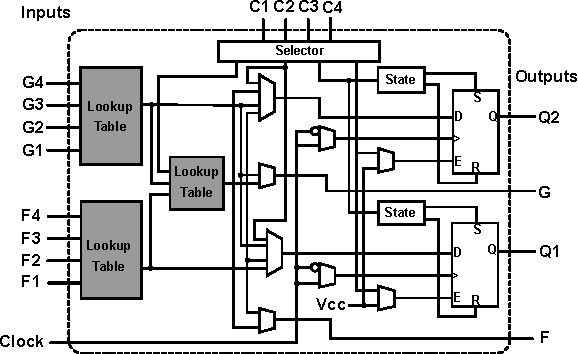
\includegraphics[width=0.8\linewidth]{figs/FPGA/CBL.pdf}
    \caption{Imagem ilustrativa de um \textit{CBL}. Adaptado de \citeonline{genera_technologies_fpga}}
    \label{fig:FPGA_CBL}
\end{figure}

Além disso, o modelo de temporização, timing, nos FPGAs é fundamental: cada sinal tem um caminho entre flip-flops, com restrições de tempo (\textit{setup}, \textit{hold}), e o roteamento de pistas e \textit{buffers} intermediários afetam a latência e taxa máxima de \textit{clock} \mbox{que pode ser alcançada.}

% \subsection*{Fluxo de Desenvolvimento com FPGA}

% Um mapeamento mais detalhado do fluxo de desenvolvimento FPGA típico, com ênfase em aplicações de IA, pode ser descrito da seguinte forma:

% \begin{enumerate}
% \item \textbf{Definição do algoritmo / modelo}
% No caso de IA, inicia-se com o projeto ou escolha da rede neural (topologia, número de camadas, tipo de ativação, quantização, compressão etc.).

% \item \textbf{Quantização / otimização de modelo}
% Para reduzir custo de hardware e latência, frequentemente aplica-se quantização (redução da largura de bits dos pesos e ativações), poda (pruning), compressão esparsa, fatoração ou aproximação de operações.

% \item \textbf{Descrição em HDL ou HLS (High-Level Synthesis)}
% A rede otimizada é então implementada usando linguagens de descrição de hardware (VHDL, Verilog) ou por meio de ferramentas HLS que compilam descrições em C/C++/OpenCL para hardware. As ferramentas HLS permitem abstração mais alta, mas exigem atenção à qualidade do hardware gerado (área, latência, paralelismo).

% \item \textbf{Síntese Lógica}
% A ferramenta converte a descrição de alto nível em uma rede de portas lógicas (LUTs, flip-flops, blocos DSP) lógicas equivalentes.

% \item \textbf{Implementação (Place & Route)}
% O mapeamento lógico é alocado em CLBs, rotas são calculadas pela ferramenta de roteamento, e as interconexões entre blocos são estabelecidas. Aqui ocorrem problemas de congestionamento e restrições de tempo.

% \item \textbf{Análise de Tempo e Ajustes}
% Após roteamento, é feita análise estática de tempo para verificar se os caminhos críticos atendem às restrições de clock. Caso contrário, ajusta-se pipeline, duplicação de lógica, re-rastro, bufferização, restrições de roteamento etc.

% \item \textbf{Geração do Bitstream e Programação}
% O arquivo de configuração (bitstream) é gerado e carregado no FPGA, configurando a interconexão e lógica conforme o design projetado.

% \item \textbf{Verificação / Validação / Testes em Hardware}
% Finalmente, testa-se o circuito configurado (validação funcional, testes de desempenho, consumo, latência, estabilidade).

% \item \textbf{Iterações / Otimizações}
% Muitas vezes, múltiplas iterações são necessárias: ajustes no modelo, re-quantização, pipeline mais fino, divisão em blocos, paralelismo, balanceamento de carga, uso de memória local etc.

% \end{enumerate}

\subsection*{Fluxo de Desenvolvimento com FPGA}

O fluxo de desenvolvimento em FPGAs segue uma sequência bem definida de etapas, que vão desde a concepção do algoritmo até a implementação e validação física do projeto no dispositivo. Esse processo é especialmente relevante em aplicações de Inteligência Artificial (IA) e aprendizado profundo, nas quais o equilíbrio entre desempenho, consumo e utilização de recursos é determinante para a viabilidade do sistema.

O fluxo de desenvolvimento em FPGA, com ênfase em aplicações de Inteligência Artificial, pode ser descrito como uma sequência de etapas encadeadas, que vão desde a definição conceitual do modelo até a validação em hardware e as \mbox{iterações finais de otimização.}

Inicialmente, na \textbf{definição do algoritmo ou modelo}, estabelece-se o comportamento desejado do sistema digital. Em aplicações de IA, essa etapa envolve a escolha ou o projeto de uma arquitetura de rede neural adequada (por exemplo, definição do número de camadas, tipos de ativação, organização MLP e tamanho dos filtros), considerando simultaneamente requisitos de precisão, latência, uso de recursos e complexidade computacional. Trata-se de uma fase predominantemente algorítmica, na qual ainda não se impõem, de forma explícita, as restrições do dispositivo FPGA alvo.

Em seguida, ocorre a \textbf{quantização e otimização do modelo}, cujo objetivo é reduzir o custo computacional e a demanda de recursos de hardware, preservando, tanto quanto possível, a acurácia do modelo. Técnicas como quantização de pesos e ativações (redução da largura de bits), poda (\textit{pruning}), compressão esparsa e fatoração de matrizes são empregadas para diminuir o número de operações e o volume de dados trafegados. Essa etapa é particularmente crítica em FPGAs, dado que LUTs, blocos DSP e BRAMs são recursos finitos e precisam ser utilizados de forma eficiente.

A arquitetura já otimizada é então traduzida para uma \textbf{descrição em HDL ou HLS (High-Level Synthesis)}. Nessa fase, o projeto é implementado em linguagens de descrição de hardware tradicionais, como VHDL ou Verilog, ou em linguagens de mais alto nível (C/C++/OpenCL) que serão sintetizadas por ferramentas de HLS. Embora o HLS facilite o desenvolvimento e aumente o nível de abstração, ele exige uma análise cuidadosa da qualidade do hardware gerado, sobretudo no que diz respeito à área ocupada, ao grau de paralelismo explorado e à latência dos caminhos críticos.

A etapa seguinte corresponde à \textbf{sintese lógica}, na qual a descrição funcional é convertida em uma rede lógica equivalente composta por LUTs, flip-flops, blocos DSP e memórias internas (BRAMs) do FPGA. As ferramentas de síntese aplicam otimizações de lógica booleana, realizam o mapeamento para os recursos específicos do dispositivo e geram uma representação intermediária que servirá de base para o \mbox{processo de implementação física.}

Concluída a síntese, procede-se à \textbf{implementação física (\textit{place \& route})}. Nessa fase, os elementos lógicos são posicionados na matriz do FPGA (\textit{placement}) e as conexões elétricas entre eles são estabelecidas (\textit{routing}). A forma como os blocos (CLBs, DSPs, BRAMs) são distribuídos e interligados impacta diretamente a frequência máxima de operação e o consumo de energia. Congestionamentos na rede de interconexão ou rotas excessivamente longas podem impedir o cumprimento das metas de \mbox{temporização definidas no projeto.}

Após o roteamento, realiza-se a \textbf{análise de tempo e o \textit{timing closure}}. Por meio de análise estática de temporização, verificam-se as restrições de \textit{setup} e \textit{hold} em todos os caminhos relevantes. Caso os caminhos críticos excedam o período de clock especificado, torna-se necessário aplicar técnicas de otimização, tais como inserção de estágios adicionais de pipeline, replicação de lógica, refinamento de restrições ou reorganização de blocos. O objetivo é garantir que o design opere de forma confiável na frequência alvo.

Uma vez satisfeitas as restrições de temporização, procede-se à \textbf{geração do bitstream e programação do dispositivo}. A configuração final é codificada em um arquivo de bits (\textit{bitstream}) que descreve completamente a interconexão e o comportamento interno do FPGA. Esse arquivo é então carregado no dispositivo por meio de interfaces apropriadas (como JTAG, SPI ou USB), configurando-o conforme o projeto desenvolvido.

Na sequência, ocorre a fase de \textbf{verificação e testes em hardware}, em que o design é validado fisicamente no FPGA. São realizados testes funcionais, medições de desempenho, análise de estabilidade e avaliação do consumo energético. Em aplicações de IA, é usual executar a inferência diretamente no hardware, comparando-se a acurácia e o tempo de resposta com aqueles obtidos em simulação ou em plataformas de referência (CPU/GPU), especialmente após a quantização e outras otimizações.

Por fim, o processo raramente se encerra em uma única passagem. Assim, fala-se em \textbf{iterações e otimizações finais}, nas quais o projetista retorna a etapas anteriores para ajustar parâmetros, refinar o pipeline, melhorar o paralelismo, reorganizar \textit{buffers} de memória local e equilibrar a utilização de recursos lógicos e de comunicação. Esse ciclo iterativo é característico do desenvolvimento em FPGA e permite gradualmente aproximar o projeto dos requisitos almejados de latência, \textit{throughput}, \mbox{consumo de energia e área ocupada.}


%O fluxo de desenvolvimento em FPGAs segue uma sequência bem definida de etapas, que vão desde a concepção do algoritmo até a implementação e validação física do projeto no dispositivo. Esse processo, representado de forma resumida na Tabela~\ref{tab:fluxo_fpga}, é especialmente relevante em aplicações de Inteligência Artificial (IA) e aprendizado profundo, nas quais o equilíbrio entre desempenho, consumo e utilização de recursos é determinante para a viabilidade do sistema.

%\begin{table}[H]
%\centering
%\caption{Etapas típicas do fluxo de desenvolvimento em FPGA, com ênfase em aplicações de Inteligência Artificial.}
%\label{tab:fluxo_fpga}
%\renewcommand{\arraystretch}{1.3}
%\resizebox{\textwidth}{!}{%
%\begin{tabular}{p{4cm} p{12cm}}
%\hline
%\textbf{Etapa} & \textbf{Descrição e Objetivos Principais} \\ \hline
%
%\textbf{1. Definição do Algoritmo ou Modelo} &
%Corresponde à etapa inicial do projeto, na qual se define o comportamento desejado do sistema digital. Em aplicações de IA, envolve a escolha ou o desenvolvimento de uma arquitetura de rede neural (número de camadas, tipo de ativação, estrutura MLP, etc.), levando em conta requisitos de precisão, latência e complexidade. \\ \hline
%
%\textbf{2. Quantização e Otimização do Modelo} &
%Visa reduzir a complexidade computacional e o consumo de recursos do FPGA. Técnicas como quantização (redução da largura de bits de pesos e ativações), poda (\textit{pruning}), compressão esparsa e fatoração de matrizes são aplicadas para otimizar o desempenho e minimizar a latência sem comprometer a acurácia do modelo. \\ \hline
%
%\textbf{3. Descrição em HDL ou HLS (High-Level Synthesis)} &
%A arquitetura otimizada é implementada em uma linguagem de descrição de hardware (VHDL, Verilog) ou em linguagens de alto nível (C/C++/OpenCL) compiladas por ferramentas de \textit{High-Level Synthesis}. O HLS facilita o desenvolvimento, mas requer análise criteriosa da qualidade do hardware gerado, especialmente em termos de área, paralelismo e latência. \\ \hline
%
%\textbf{4. Síntese Lógica} &
%Converte a descrição funcional em uma rede lógica equivalente composta por LUTs, flip-flops, blocos DSP e BRAMs. Nessa etapa são aplicadas otimizações automáticas de lógica booleana e mapeamento de recursos específicos do dispositivo alvo. \\ \hline
%
%\textbf{5. Implementação (Place \& Route)} &
%Os elementos lógicos são fisicamente mapeados na matriz do FPGA. O processo de \textit{placement} define a alocação espacial dos blocos (CLBs, DSPs, BRAMs), enquanto o \textit{routing} estabelece as conexões elétricas entre eles. Essa fase é crítica para o desempenho, pois o congestionamento ou roteamento inadequado pode limitar a frequência máxima de operação. \\ \hline
%
%\textbf{6. Análise de Tempo e Ajustes (Timing Closure)} &
%Após o roteamento, é realizada a análise estática de tempo, que verifica o cumprimento das restrições de temporização (\textit{setup} e \textit{hold}). Caso os caminhos críticos ultrapassem o período de clock, aplicam-se técnicas de otimização, como inserção de pipeline, replicação de lógica e ajustes de restrições. \\ \hline
%
%\textbf{7. Geração do Bitstream e Programação} &
%A configuração final é traduzida em um arquivo de bits (\textit{bitstream}), responsável por definir a interconexão e o comportamento interno do FPGA. Esse arquivo é então carregado no dispositivo por meio de interfaces JTAG, SPI ou USB, configurando-o conforme o projeto desenvolvido. \\ \hline
%
%\textbf{8. Verificação e Testes em Hardware} &
%Nesta fase, o design é validado fisicamente. São realizados testes de funcionalidade, desempenho, estabilidade e consumo energético. Em projetos de IA, é comum realizar inferência direta no FPGA para medir a precisão do modelo após quantização e integração. \\ \hline
%
%\textbf{9. Iterações e Otimizações Finais} &
%O ciclo de desenvolvimento raramente é linear. Geralmente, diversas iterações são necessárias para ajustar parâmetros, refinar o pipeline, melhorar o paralelismo, reorganizar buffers de memória local e equilibrar a utilização de recursos lógicos e de comunicação. \\ \hline
%\end{tabular}}
%\end{table}

O processo de desenvolvimento e otimização de projetos em FPGA pode ser sintetizado na Figura~\ref{fig:FluxoDesenvolvimentoFPGA}, que apresenta, de forma esquemática, o ciclo completo desde a definição inicial do algoritmo até a validação em hardware. Esse fluxo evidencia o caráter iterativo do desenvolvimento em dispositivos reconfiguráveis, no qual a cada etapa — da modelagem à implementação física — o projetista deve buscar o equilíbrio entre desempenho, \mbox{consumo e utilização de recursos lógicos.}

\begin{figure}[H]
    \centering
    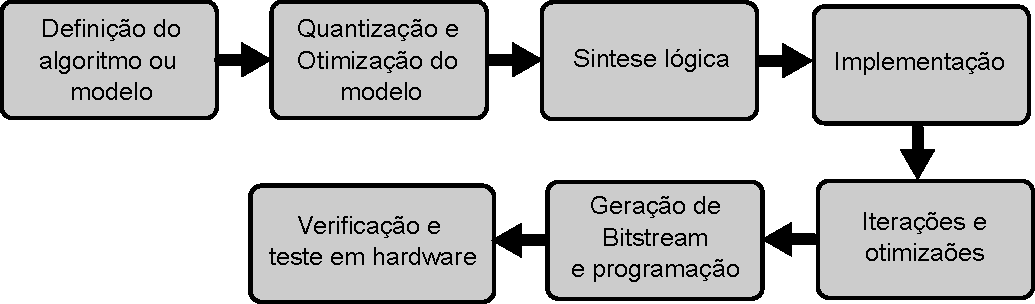
\includegraphics[width=0.8\linewidth]{figs/FPGA/FluxoOtimização.pdf}
    \caption{Fluxo de desenvolvimento e otimização de projetos em FPGA. O autor.}
    \label{fig:FluxoDesenvolvimentoFPGA}
\end{figure}

A Figura~\ref{fig:FluxoDesenvolvimentoFPGA} destaca a sequência típica de etapas: inicia-se pela definição do modelo ou algoritmo, seguida pela quantização e otimização, que reduzem a complexidade computacional. Na sequência, a descrição em HDL ou por meio de ferramentas de HLS permite traduzir o comportamento algorítmico em lógica digital reconfigurável. As fases de síntese e \textit{place \& route} realizam o mapeamento físico do projeto sobre os blocos lógicos e interconexões do FPGA, seguidas da análise de temporização, responsável por assegurar que todas as restrições de tempo de propagação sejam satisfeitas. Por fim, ocorre a geração do \textit{bitstream}, etapa na qual o projeto é convertido em um arquivo de configuração e carregado no dispositivo para verificação e validação funcional.

Ao final do ciclo, ajustes e otimizações adicionais são frequentemente necessários, refletindo o caráter experimental e aprimorável do processo. Essa natureza iterativa é fundamental em aplicações de Inteligência Artificial, nas quais a eficiência do hardware depende diretamente do grau de paralelismo, da largura de barramento e da arquitetura da rede neural mapeada no FPGA.


O sucesso do projeto depende da integração eficiente entre as etapas de síntese, implementação e análise de tempo. Pequenas variações no roteamento ou na granularidade do paralelismo podem impactar significativamente a taxa máxima de \textit{clock} e o consumo energético do sistema, sobretudo em aplicações de aprendizado profundo com restrições de latência e \textit{throughput}.

No contexto de aplicações de Inteligência Artificial, algumas etapas do fluxo de desenvolvimento em FPGA exigem atenção especial para garantir eficiência e desempenho. O \textit{quantization-aware training}, por exemplo, permite que o modelo seja treinado levando em consideração os efeitos da quantização, preservando a acurácia mesmo com representações de baixa precisão. O mapeamento eficiente de multiplicações binárias ou quantizadas — frequentemente implementadas em blocos DSP — é essencial para maximizar o paralelismo e reduzir o consumo de área lógica. Da mesma forma, o suporte à ``esparsidade'' de valores nulos e a utilização otimizada de memórias locais (BRAM e URAM) são fatores decisivos para minimizar a dependência de acessos à memória externa, os quais representam um dos principais gargalos de desempenho em arquiteturas reconfiguráveis.  

Essas estratégias de otimização, quando bem empregadas, tornam os FPGAs especialmente adequados para aplicações embarcadas de IA e aprendizado profundo, nas quais o equilíbrio entre consumo energético, latência e throughput é determinante para a viabilidade prática do sistema.

% A subseção a seguir apresenta uma análise comparativa das principais vantagens e limitações desses dispositivos, considerando seu uso em aceleração de algoritmos de inteligência artificial.

%\subsection*{Vantagens e Desvantagens dos FPGAs (na perspectiva de IA)}
%
%O uso de FPGAs em aplicações de Inteligência Artificial apresenta um conjunto de vantagens que os torna particularmente atrativos para a implementação de algoritmos de aprendizado profundo e de processamento de sinais em tempo real. Em especial, destacam-se aspectos como flexibilidade de reconfiguração, exploração de paralelismo em nível de hardware e potencial de eficiência energética em cenários de inferência embarcada e de borda, \textit{edge computing}. A seguir, são sintetizados alguns dos principais pontos fortes associados a essa tecnologia:
%
%\begin{itemize}
%	\item \textbf{Reconfigurabilidade e adaptabilidade:} possibilita modificar o hardware após a fabricação, permitindo ajustar a arquitetura à medida que o modelo de IA ou os requisitos do sistema evoluem, sem necessidade de projetar um novo circuito integrado dedicado.
%	
%	\item \textbf{Paralelismo massivo:} os recursos lógicos internos permitem a execução simultânea de múltiplas operações, explorando de forma direta o paralelismo intrínseco de redes neurais, filtros convolucionais e demais blocos de processamento distribuído.
%	
%	\item \textbf{Baixa latência e previsibilidade temporal:} a ausência de camadas intermediárias de software e de sistemas operacionais complexos favorece um comportamento determinístico, com latência reduzida e previsível — característica essencial em aplicações em tempo real e em sistemas de controle crítico.
%	
%	\item \textbf{Eficiência energética:} quando adequadamente otimizados, projetos em FPGA podem alcançar maior eficiência em termos de operações por joule (ops/J) do que soluções baseadas exclusivamente em GPU, especialmente em cenários de inferência local e dispositivos de borda.
%	
%	\item \textbf{Customização de precisão:} o suporte à implementação de operações com diferentes larguras de palavra (por exemplo, formatos binários, ternários ou de 4–8 bits) permite ajustar o uso de recursos de hardware de acordo com a tolerância do modelo à quantização, equilibrando acurácia e custo computacional.
%	
%	\item \textbf{Integração de funções heterogêneas:} em um único chip, é possível combinar blocos de controle, interfaces de comunicação, módulos de pré-processamento e pós-processamento de sinais, reduzindo a latência de comunicação entre etapas e o consumo global do sistema.
%\end{itemize}


%O uso de FPGAs em aplicações de Inteligência Artificial apresenta um conjunto de vantagens que os tornam altamente atrativos para a implementação de algoritmos de aprendizado profundo e processamento de sinais em tempo real. A Tabela~\ref{tab:fpga_vantagens} sintetiza os principais aspectos positivos observados na literatura e na prática industrial, destacando sua flexibilidade, paralelismo e eficiência energética — fatores determinantes para aplicações embarcadas e de borda (\textit{edge computing}).
%
%\begin{table}[H]
%\centering
%\caption{Principais vantagens dos FPGAs em aplicações de Inteligência Artificial.}
%\label{tab:fpga_vantagens}
%\renewcommand{\arraystretch}{1.3}
%\resizebox{\textwidth}{!}{%
%\begin{tabular}{p{4cm} p{12cm}}
%\hline
%\textbf{Vantagem} & \textbf{Descrição} \\ \hline
%
%\textbf{Reconfigurabilidade e adaptabilidade} &
%Permite modificar o hardware após a fabricação, possibilitando ajustes à medida que o modelo ou os requisitos do sistema evoluem, sem a necessidade de novos projetos físicos. \\ \hline
%
%\textbf{Paralelismo massivo} &
%Os recursos lógicos permitem a execução simultânea de múltiplas operações, explorando o paralelismo intrínseco de redes neurais e filtros convolucionais. \\ \hline
%
%\textbf{Baixa latência e previsibilidade temporal} &
%A ausência de camadas intermediárias de software garante processamento determinístico, ideal para aplicações em tempo real e controle crítico. \\ \hline
%
%\textbf{Eficiência energética} &
%Projetos bem otimizados em FPGA podem atingir maior eficiência em operações por joule (ops/J) do que GPUs, especialmente em aplicações de inferência local e dispositivos de borda. \\ \hline
%
%\textbf{Customização de precisão} &
%Suporte à implementação de operações com diferentes larguras de palavra (binária, ternária, 4–8 bits), ajustando o consumo de recursos conforme a tolerância do modelo à quantização. \\ \hline
%
%\textbf{Integração de funções heterogêneas} &
%Permite integrar, em um único chip, blocos de controle, interfaces de comunicação, pré-processamento e pós-processamento de sinais, reduzindo latência e consumo. \\ \hline
%\end{tabular}}
%\end{table}

%Apesar de seus benefícios, o uso de FPGAs em aplicações de Inteligência Artificial também apresenta limitações e desafios que precisam ser cuidadosamente considerados no processo de projeto. Em particular, destacam-se restrições de recursos físicos, maior complexidade de desenvolvimento e um ciclo de projeto mais longo quando comparado a plataformas mais convencionais. A seguir, são sintetizados alguns dos principais pontos críticos associados a essa tecnologia:
%
%\begin{itemize}
%	\item \textbf{Recursos limitados:} a quantidade de blocos lógicos, unidades DSP e memórias internas (BRAMs) disponível em um FPGA é finita. Redes neurais de grande porte ou modelos com elevado número de parâmetros podem exceder a capacidade do dispositivo, exigindo estratégias adicionais de quantização, poda ou \mbox{particionamento do modelo.}
%	
%	\item \textbf{Complexidade de projeto:} o desenvolvimento em FPGA demanda domínio de linguagens de descrição de hardware (como VHDL e Verilog) ou de fluxos baseados em \textit{High-Level Synthesis}, além de conhecimento em síntese lógica, fechamento de temporização e otimização de desempenho. Esse conjunto de competências torna a curva de aprendizado mais íngreme quando comparado a frameworks de alto nível em CPU ou GPU.
%	
%	\item \textbf{Desempenho inferior a ASICs dedicados:} embora ofereçam flexibilidade e reconfigurabilidade, FPGAs não alcançam, em geral, a mesma densidade lógica nem a mesma eficiência energética de circuitos integrados de aplicação específica (ASICs) projetados sob medida para uma determinada rede ou tarefa.
%	
%	\item \textbf{Consumo em uso contínuo:} em aplicações de longa duração e alta taxa de utilização, o consumo energético total pode superar o de soluções especializadas ou de chips dedicados, sobretudo quando o projeto não explora plenamente recursos de desligamento parcial, \textit{clock gating} ou outras técnicas de economia de energia.
%	
%	\item \textbf{Tempo de desenvolvimento elevado:} etapas como implementação física, \textit{place \& route}, fechamento de temporização, \textit{timing closure}, balanceamento de pipeline e ajuste fino de restrições podem demandar múltiplas iterações, aumentando significativamente o tempo total de desenvolvimento em comparação com arquiteturas puramente de software.
%	
%	\item \textbf{Gargalos de memória externa:} o acesso frequente à memória DRAM externa pode introduzir latência adicional e elevar o consumo de energia. Isso exige estratégias cuidadosas de uso de memória local (BRAMs, buffers e caches) e de reutilização de dados para evitar que a banda de memória se torne o \mbox{principal limitante do desempenho.}
%	
%	\item \textbf{Desafios de quantização e precisão:} a necessidade de reduzir a largura de palavra (por exemplo, para 8, 4 ou até 1–2 bits) a fim de caber no FPGA pode conduzir à degradação da acurácia do modelo. Encontrar o equilíbrio entre custo de hardware e desempenho preditivo é uma tarefa não trivial, frequentemente exigindo técnicas de \textit{quantization-aware training} e experimentação extensiva.
%\end{itemize}


%Apesar de seus benefícios, o uso de FPGAs também apresenta limitações que devem ser consideradas durante o processo de desenvolvimento. Conforme resumido na Tabela~\ref{tab:fpga_desvantagens}, os principais desafios envolvem restrições de recursos físicos, complexidade de projeto, e tempo de desenvolvimento — fatores que demandam conhecimento especializado em arquitetura digital e ferramentas de síntese.
%
%\begin{table}[H]
%\centering
%\caption{Principais desvantagens e desafios no uso de FPGAs para aplicações de IA.}
%\label{tab:fpga_desvantagens}
%\renewcommand{\arraystretch}{1.3}
%\resizebox{\textwidth}{!}{%
%\begin{tabular}{p{4cm} p{12cm}}
%\hline
%\textbf{Desvantagem} & \textbf{Descrição} \\ \hline
%
%\textbf{Recursos limitados} &
%A quantidade de blocos lógicos, DSPs e memórias internas é finita; redes neurais de grande porte podem exceder a capacidade disponível. \\ \hline
%
%\textbf{Complexidade de projeto} &
%O desenvolvimento requer domínio de linguagens de descrição de hardware (VHDL, Verilog) e ferramentas de síntese, além de experiência com restrições temporais e otimização de performance. \\ \hline
%
%\textbf{Desempenho inferior a ASICs} &
%Embora flexível, o FPGA não atinge a mesma densidade lógica nem a eficiência energética de um ASIC dedicado para a mesma aplicação. \\ \hline
%
%\textbf{Consumo em uso contínuo} &
%Para tarefas de longa duração, o consumo energético pode superar soluções otimizadas ou chips dedicados. \\ \hline
%
%\textbf{Tempo de desenvolvimento elevado} &
%Etapas como roteamento, fechamento de temporização (\textit{timing closure}) e balanceamento de pipeline aumentam significativamente o tempo de iteração. \\ \hline
%
%\textbf{Gargalos de memória externa} &
%O acesso à memória DRAM externa pode introduzir latência e elevar o consumo de energia, exigindo estratégias de uso eficiente da memória local. \\ \hline
%
%\textbf{Desafios de quantização e precisão} &
%A redução excessiva da precisão pode degradar a acurácia do modelo; equilibrar custo de hardware e desempenho é uma tarefa complexa. \\ \hline
%\end{tabular}}
%\end{table}

%Diante desse conjunto de vantagens e limitações, o uso de FPGAs em aplicações de Inteligência Artificial caracteriza-se por um claro compromisso entre desempenho, flexibilidade e complexidade de desenvolvimento. 
%
%Por um lado, a possibilidade de explorar paralelismo em nível de hardware, customizar a precisão numérica e integrar, em um único dispositivo, funções de aquisição, processamento e decisão torna os FPGAs particularmente atraentes para sistemas de monitoramento em tempo real baseados em aprendizado de máquina. Por outro, a necessidade de lidar com recursos restritos, fluxos de projeto mais complexos e desafios de quantização demanda uma fase prévia de estudo e modelagem cuidadosa antes de se partir para a implementação física. 
%
%Nesse contexto, o presente trabalho concentra-se em um \textit{estudo de viabilidade} por meio de simulação de uma arquitetura baseada em rede MLP embarcada em FPGA, utilizando o framework FINN como ferramenta de apoio ao mapeamento em hardware.
%



%O objetivo é compreender, de forma sistemática, como os trade-offs entre acurácia, latência e uso de recursos podem ser equilibrados em um cenário de detecção de cavitação por emissão acústica, fornecendo subsídios técnicos para futuras etapas de prototipagem e implementação real.


\subsection{Otimização de IA em FPGAs: técnicas, desafios e tendências}

Para que redes neurais sejam mapeadas de forma eficiente em FPGAs, é necessário aplicar um conjunto de técnicas de otimização que atuam simultaneamente sobre a arquitetura do modelo, a representação numérica dos dados e a própria organização interna do hardware, garantindo assim um melhor aproveitamento dos recursos disponíveis.

Em linhas gerais, essas estratégias buscam reduzir latência, consumo de energia e uso de área lógica, preservando, tanto quanto possível, a acurácia do modelo. A seguir, são apresentadas algumas das principais abordagens relatadas na literatura recente para aceleração de redes neurais em FPGAs:

\begin{itemize}
	\item \textbf{Quantização:} consiste em reduzir a largura de bits de pesos e ativações (por exemplo, para 8, 4, 2 ou mesmo 1 bit), diminuindo o uso de DSPs e de memória interna. Quando combinada com treinamento ciente de quantização (\textit{quantization-aware training}), essa técnica permite obter modelos mais compactos com perda limitada de desempenho, sendo uma das bases de muitos fluxos de implementação em FPGA.
	
	\item \textbf{Poda e exploração de esparsidade:} remove conexões cujos pesos são próximos de zero, reduzindo o número de operações aritméticas e acessos à memória. Para que o ganho seja efetivo em hardware, é necessário que a arquitetura seja projetada para explorar essa esparsidade de maneira estruturada, evitando \textit{overheads} de controle que anulam o benefício.
	
	\item \textbf{Fusão de camadas e compressão de operadores:} integra operações que, tradicionalmente, seriam tratadas de forma separada — como convolução, ativação e \textit{pooling}, em um único bloco funcional. Essa fusão diminui o tráfego de dados entre módulos, reduz a lógica de interconexão e pode simplificar o roteamento e o controle do fluxo de informações.
	
	\item \textbf{Fatoração e decomposição de operações:} convoluções maiores (como filtros \(3\times3\) ou \(5\times5\)) podem ser decompostas em operações menores ou sequenciais, de forma a economizar recursos lógicos e facilitar o fechamento de temporização. Em alguns casos, decomposições separáveis (espacial ou em canais) permitem diminuir significativamente o custo computacional.
	
	\item \textbf{Pipeline e paralelismo fino:} divide-se o processamento em múltiplos estágios de pipeline, permitindo que diferentes amostras ou partes do cálculo sejam processadas simultaneamente em fases distintas. Esse paralelismo fino, típico de arquiteturas \textit{streaming}, contribui para manter o \textit{throughput} elevado com latência de \mbox{cada estágio controlada.}
	
	\item \textbf{Uso eficiente de memória local:} maximiza-se o aproveitamento de BRAMs, URAMs e \textit{buffers} internos para reduzir a dependência da DRAM externa. Estratégias de \textit{tiling}, reutilização de dados e armazenamento em janelas deslizantes são fundamentais para evitar que o gargalo de memória se torne o \mbox{principal limitante do desempenho.}
	
	\item \textbf{Compressão e codificação de pesos:} emprega técnicas como compressão \textit{run-length} e codificação de comprimento variável para reduzir o tamanho do modelo e o volume de dados transferidos. Em combinação com sparsidade, essa abordagem contribui para diminuir a largura de banda necessária entre memória e \mbox{unidades de processamento.}
	
	\item \textbf{Aritmética aproximada:} substitui operações exatas por variantes aproximadas (por exemplo, somadores e multiplicadores aproximados), com menor custo de implementação. Desde que o erro introduzido permaneça dentro de limites aceitáveis para a aplicação, é possível reduzir significativamente área, \mbox{latência e consumo energético.}
	
	\item \textbf{Arquiteturas \textit{dataflow} e \textit{streaming}:} modelam a rede neural como um fluxo contínuo de dados que atravessa uma sequência de operadores, ao invés de um conjunto de camadas executadas de forma estritamente sequencial e armazenadas em memória. Essa visão \textit{dataflow} permite eliminar gargalos de sincronização, explorar paralelismo em nível de fluxo e alinhar melhor o modelo ao \mbox{estilo de computação dos FPGAs.}
	
	\item \textbf{Reconfiguração parcial dinâmica:} possibilita reprogramar seletivamente regiões do FPGA em tempo de execução, permitindo, por exemplo, alternar entre diferentes sub-redes ou modos de operação sem reconfigurar todo o dispositivo. Essa técnica ajuda a reutilizar recursos em cenários em que não é possível manter toda a funcionalidade residente simultaneamente.
	
	\item \textbf{Co-design hardware--software:} distribui as funções do sistema entre a lógica reconfigurável e um processador embutido (em plataformas SoC), buscando um ponto de equilíbrio entre custo de hardware, latência e flexibilidade. Operações de controle, pré-processamento ou pós-processamento podem permanecer em software, enquanto o núcleo do cálculo numérico é acelerado no FPGA.
\end{itemize}


%Para que redes neurais sejam eficientemente mapeadas em FPGAs, diversas técnicas de otimização são empregadas, com foco em reduzir a latência, o consumo de energia e o uso de área lógica, mantendo a acurácia do modelo. A Tabela~\ref{tab:fpga_otimizacao_tecnicas} sintetiza as principais estratégias relatadas na literatura recente, destacando como cada uma contribui para o desempenho geral do sistema.
%
%\begin{table}[H]
%\centering
%\caption{Principais técnicas de otimização aplicadas a redes neurais em FPGAs.}
%\label{tab:fpga_otimizacao_tecnicas}
%\renewcommand{\arraystretch}{1.3}
%\resizebox{\textwidth}{!}{%
%\begin{tabular}{p{4cm} p{12cm}}
%\hline
%\textbf{Técnica} & \textbf{Descrição e objetivo principal} \\ \hline
%
%\textbf{Quantização} &
%Reduz a largura de bits de pesos e ativações (ex.: 8, 4, 2 ou 1 bit), minimizando uso de DSPs e memória. Mantém boa acurácia quando combinada com treinamento ciente de quantização (\textit{quantization-aware training}). \\ \hline
%
%\textbf{Poda / Sparsidade} &
%Remove conexões com pesos próximos de zero, diminuindo a quantidade de operações e acessos à memória. Exige arquiteturas otimizadas para explorar a sparsidade de forma eficiente. \\ \hline
%
%\textbf{Fusão de camadas / Compressão de operadores} &
%Combina operações consecutivas (convolução, ativação e pooling) para reduzir o tráfego de dados e a sobrecarga de lógica de interconexão. \\ \hline
%
%\textbf{Fatoração / Decomposição} &
%Divide grandes convoluções (como 3×3 ou 5×5) em operações menores ou sequenciais, economizando recursos lógicos e simplificando o roteamento. \\ \hline
%
%\textbf{Pipeline e paralelismo fino} &
%Implementa execução sobreposta de múltiplas etapas e divide operações em estágios curtos, garantindo throughput constante e baixa latência. \\ \hline
%
%\textbf{Uso eficiente de memória local} &
%Reduz dependência da DRAM externa, maximizando reutilização de dados via BRAM/URAM e buffers de streaming interno. \\ \hline
%
%\textbf{Compressão e codificação de pesos} &
%Emprega técnicas como compressão \textit{run-length} e codificação de comprimento variável para reduzir o tamanho do modelo e o tráfego de dados. \\ \hline
%
%\textbf{Aritmética aproximada} &
%Substitui operações exatas por versões aproximadas para diminuir o custo computacional, mantendo o erro dentro de limites aceitáveis. \\ \hline
%
%\textbf{Arquiteturas \textit{dataflow} e \textit{streaming}} &
%Modelam a rede como um fluxo contínuo de dados, maximizando o paralelismo e eliminando gargalos de sincronização entre camadas. \\ \hline
%
%\textbf{Reconfiguração parcial dinâmica} &
%Permite reprogramar seletivamente partes do FPGA em tempo de execução, otimizando uso de recursos para diferentes fases do modelo. \\ \hline
%
%\textbf{Co-design hardware-software} &
%Distribui funções entre lógica reconfigurável (FPGA) e processador embutido (SoC), equilibrando custo, latência e consumo energético. \\ \hline
%\end{tabular}}
%\end{table}

Diversos estudos e \textit{surveys} analisam essas estratégias sob diferentes perspectivas, comparando \textit{frameworks} e abordagens de implementação. A Tabela~\ref{tab:otimizacao_mlp_fpga} apresenta um resumo de publicações recentes que investigam técnicas de aceleração de redes neurais em FPGAs, destacando o foco principal e as contribuições de cada estudo.

%\begin{table}[H]
%	\footnotesize
%	\centering
%	\caption{Trabalhos focados em técnicas de otimização de MLPs para implementação em hardware reconfigurável (FPGA).}
%	\label{tab:otimizacao_mlp_fpga}
%	\renewcommand{\arraystretch}{1.3}
%	\resizebox{\textwidth}{!}{%
%		\begin{tabular}{p{3.5cm} p{3.5cm} p{5cm} p{3cm}}
%			\hline
%			\textbf{Técnica de Otimização} & \textbf{Objetivo da Otimização} & \textbf{Abordagem e Resultados} & \textbf{Referência} \\ \hline
%			
%			\textbf{Quantização e Ponto Fixo} & Redução de uso de memória e DSPs & Substituição de aritmética de ponto flutuante (32-bit) por ponto fixo customizado (ex: 8-bit ou 16-bit) com perda mínima de acurácia (<1\%). & \citeonline{toumi2022fpga} \\ \hline
%			
%			\textbf{Paralelismo de Neurônios} & Aumento do \textit{Throughput} & Implementação de múltiplas unidades de multiplicação e acumulação (MAC) operando em paralelo para processar uma camada inteira em poucos ciclos de clock. & \citeonline{Gadea2017} \\ \hline
%			
%			\textbf{Aproximação de Funções de Ativação} & Redução de custo computacional & Uso de tabelas de busca (LUTs) ou aproximação por séries de Taylor/CORDIC para calcular Sigmoide e Tangente Hiperbólica sem usar recursos exponenciais. & \citeonline{Bezerra2021} \\ \hline
%			
%			\textbf{Arquitetura em Pipeline} & Redução de Latência & Segmentação das camadas da MLP em estágios de pipeline, permitindo que a rede processe novos dados de entrada antes mesmo de finalizar a classificação anterior. & \citeonline{shreejith2016} \\ \hline
%			
%			\textbf{Poda de Conexões (\textit{Pruning})} & Economia de Área (Lógica) & Remoção de pesos sinápticos próximos a zero após o treinamento, reduzindo o número de multiplicadores necessários na síntese do hardware. & \citeonline{Han2016} \\ \hline
%	\end{tabular}}
%\end{table}

\begin{table}[H]
	\footnotesize
	\centering
	\caption{Artigos relevantes sobre otimização e implementação de MLP ou arquiteturas similares em FPGA. Fonte: O autor.}
	\label{tab:mlp_fpga_optimization}
	\renewcommand{\arraystretch}{1.3}
	\resizebox{\textwidth}{!}{%
		\begin{tabular}{p{3cm} p{2.8cm} p{5.0cm} p{5.0cm} p{2.8cm}}
			\hline
			\textbf{Título / Trabalho} &
			\textbf{Ano} &
			\textbf{Foco de Otimização} &
			\textbf{Abordagem / Resultado} &
			\textbf{Referência} \\ \hline
			
			MLP Resource Estimation for FPGA (hls4ml) &
			2025 &
			Estimativa rápida de recursos para MLP &
			Proposta de estimador de recursos (LUT, FF, DSP) para MLPs geradas via fluxo hls4ml, acelerando a exploração de projeto antes da síntese final em FPGA. &
			\citeonline{kokkinis2025fast} \\ \hline
			
			FPGA implementation of a bearing fault classification system based on an envelope analysis and artificial neural network & 2022 & Redução de uso de memória e DSPs & Substituição de aritmética de ponto flutuante (32-bit) por ponto fixo customizado (ex: 8-bit ou 16-bit) com perda mínima de acurácia (<1\%). & \citeonline{toumi2022fpga} \\ \hline
			
			Experimental implementation of a neural network optical channel equalizer in restricted hardware using pruning and quantization &
			2021 &
			Pruning e quantização para reduzir complexidade de MLP &
			Aplica poda (pruning) e quantização a um equalizador baseado em MLP, reduzindo a memória em até 87,12\% e a complexidade computacional em até 78,34\% sem degradação de desempenho. &
			\citeonline{ron2022experimental} \\ \hline
			
			Power and Accuracy of Multi-Layer Perceptrons (MLPs) under Reduced-voltage FPGA BRAMs Operation &
			2020 &
			Eficiência energética via undervolting &
			Estudo de operação com tensão reduzida em BRAM para economizar energia em implementações MLP em FPGA, com monitoramento de impacto na precisão da rede. &
			\citeonline{salami2020power} \\ \hline
			
			Neural Networks on FPGA com função de ativação otimizada &
			2020 &
			Função de ativação amigável ao hardware (D-ReLU) e quantização &
			Implementação de MLP com funções de ativação projetadas para reduzir uso de área em FPGA, mantendo precisão com redução de bitwidth de dados e pesos. &
			\citeonline{si2020neural} \\ \hline
			
			AutoML para MLP + FPGA co-design &
			2020 &
			Co-design e otimização automática de arquitetura &
			Fluxo de design que gera automaticamente redes MLP otimizadas e hardware FPGA correspondente, alcançando maior eficiência/throughput que implementações convencionais. &
			\citeonline{colangelo2020automl} \\ \hline
			
			FPGA-implementation of high-speed MLP neural network &
			2011 &
			Paralelismo e pipeline para MLP &
			Proposta de arquitetura pipeline paralela para MLP que reduz o caminho crítico e aumenta a frequência de operação, demonstrando desempenho superior a arquiteturas convencionais. &
			\citeonline{bahoura2011fpga} \\ \hline
			

			
	\end{tabular}}
\end{table}


%
%\begin{table}[H]
%\centering
%\footnotesize
%\caption{Trabalhos recentes sobre otimização e aceleração de IA em FPGAs. Fonte: O autor. \textcolor{red}{Vou colocar referências sobre MLP}}
%\label{tab:fpga_otimizacao_trabalhos}
%\renewcommand{\arraystretch}{1.3}
%\resizebox{\textwidth}{!}{%
%\begin{tabular}{p{4cm} p{5cm} p{7cm}}
%\hline
%\textbf{Referência} & \textbf{Foco principal} & \textbf{Contribuição / Destaque} \\ \hline
%
%\citeonline{yan2024survey} &
%Survey de aceleração de algoritmos de aprendizado de máquina em hardware &
%Analisa tendências recentes de implementação de ML em FPGAs, destacando que 81\% dos estudos abordam inferência e apenas 13\% tratam de treinamento em hardware. \\ \hline
%
%\citeonline{wang2024review} &
%Implementação de MLP em FPGA &
%Discute desafios de mapeamento, uso de memória e estratégias de computação paralela para aumentar o throughput. \\ \hline
%
%\citeonline{mouri2025optimizing} &
%Otimização de VGG16/VGG19 em FPGA &
%Apresenta técnicas de transferência de aprendizado e quantização para execução eficiente de MLP em FPGA usando o dataset CIFAR-10. \\ \hline
%
%\citeonline{silvano2025survey} &
%Aceleradores de \textit{deep learning} em hardware &
%Revisa tendências de co-design e integração de hardware para IA embarcada, incluindo FPGAs e ASICs. \\ \hline
%
%\citeonline{Li2023SurveyFPGA} &
%Survey sobre aceleradores FPGA para redes neurais profundas &
%Classifica métodos de compressão, quantização e análise de trade-offs entre área, consumo e latência. \\ \hline
%
%\citeonline{eleuldj2020survey} &
%Comparação de frameworks de DL em FPGA &
%Avalia ferramentas de mapeamento e frameworks (como FINN e HLS4ML), discutindo desempenho, flexibilidade e consumo. \\ \hline
%\end{tabular}}
%\end{table}

%Em síntese, os FPGAs se consolidam como uma alternativa estratégica entre a flexibilidade dos processadores convencionais (CPU/GPU) e o alto desempenho dos ASICs dedicados. Sua capacidade de reconfiguração e paralelismo massivo permite adequar o hardware às demandas específicas de cada aplicação, especialmente em sistemas embarcados e de inferência em tempo real. No entanto, essa flexibilidade vem acompanhada de desafios significativos, como maior complexidade de projeto, limitação de recursos internos e dependência de ferramentas especializadas de síntese e otimização. Assim, a escolha por uma arquitetura baseada em FPGA deve equilibrar os ganhos em desempenho e eficiência energética com o custo de desenvolvimento e a maturidade técnica necessária para sua implementação.  
%
%A evolução das aplicações de Inteligência Artificial em FPGAs tem impulsionado uma ampla gama de pesquisas voltadas à maximização da eficiência computacional desses dispositivos. Diversos estudos recentes investigam estratégias de otimização que conciliam desempenho, consumo energético e utilização de recursos lógicos, com ênfase em redes neurais convolucionais e arquiteturas quantizadas. A subseção a seguir discute essas técnicas, tendências e desafios, oferecendo uma visão panorâmica do estado da arte no mapeamento de modelos de IA em hardware reconfigurável.

Em síntese, observa-se que o avanço na implementação de algoritmos de aprendizado profundo em FPGAs depende fortemente da combinação de técnicas de quantização, poda e co-design hardware–software.

O foco atual das pesquisas está na busca por arquiteturas que conciliem desempenho, eficiência energética e flexibilidade de reconfiguração, explorando abordagens baseadas em \textit{dataflow} e reconfiguração parcial dinâmica. Além disso, há uma tendência crescente de integração entre ferramentas de alto nível, como Vivado, HLS4ML e Vitis AI, que automatizam parte do fluxo de desenvolvimento, tornando mais acessível a implementação de redes neurais complexas em hardware reconfigurável.

Essas iniciativas apontam para um futuro em que o mapeamento de IA em FPGAs será cada vez mais automatizado, portátil e adaptável às demandas de aplicações embarcadas e industriais.

Na sequência das técnicas de otimização discutidas anteriormente, esta subseção volta-se para o estudo de ferramentas e \textit{frameworks} voltados à síntese e aceleração de redes neurais em FPGAs. Entre as diversas soluções disponíveis no ecossistema atual, destacam-se aquelas desenvolvidas por fabricantes e grupos de pesquisa que buscam abstrair a complexidade do fluxo de implementação em hardware, automatizando etapas de quantização, mapeamento e geração de IPs reconfiguráveis.

\section{Implementaçao do MLP }

Do ponto de vista da implementação de Redes Neurais Multicamadas (MLP) em dispositivos do tipo FPGA, a literatura técnica e acadêmica aponta para diferentes abordagens consolidadas, cuja adoção depende de fatores como complexidade do modelo, precisão numérica desejada, consumo de recursos lógicos e tempo de desenvolvimento. Nesse contexto, observa-se que os métodos mais comumente empregados podem ser agrupados em três grandes famílias, atualmente em fase de levantamento e avaliação neste trabalho.

Uma primeira abordagem amplamente difundida consiste na utilização de ferramentas de Síntese em Alto Nível (High-Level Synthesis – HLS), como o Vitis HLS, nas quais cada camada da MLP é modelada como uma operação de produto matriz-vetor, acrescida de termos de polarização (\textit{bias}) e funções de ativação. Essa estratégia faz uso predominante de aritmética em ponto fixo, explorando os blocos DSP do FPGA para operações do tipo multiplicação-acumulação (MAC), além de técnicas de paralelismo, como \textit{loop unrolling} e \textit{pipelining}. Tal abordagem é amplamente adotada devido à boa adequação da arquitetura das MLPs à estrutura de processamento do FPGA, baseada em operações aritméticas elementares.

Uma segunda linha de implementação recorre a \textit{frameworks} HLS de mais alto nível, como o \textit{hls4ml}, que automatizam a geração de arquiteturas dedicadas para redes neurais artificiais, incluindo MLPs. Esses ambientes permitem uma rápida exploração de compromissos entre latência, uso de recursos lógicos e precisão numérica, sendo recorrentes em trabalhos recentes que investigam a estimativa e otimização de recursos para redes neurais embarcadas em FPGA.

Por fim, uma terceira abordagem consiste na implementação direta em nível de descrição de hardware (RTL), utilizando linguagens como VHDL ou Verilog, geralmente baseada em arquiteturas do tipo matriz-vetor (MVU) ou arranjos sistólicos. Embora mais trabalhosa, essa alternativa oferece maior controle sobre a microarquitetura do sistema, permitindo detalhamento explícito de aspectos como organização de buffers, paralelismo interno, quantização numérica e fechamento de temporização (\textit{timing closure}), sendo particularmente atrativa em contextos acadêmicos nos quais se busca uma análise aprofundada da arquitetura implementada.

Diante dessas possibilidades, o presente trabalho encontra-se em fase de levantamento e análise comparativa de artigos e teses que tratam da implementação eficiente de MLPs em FPGA, com o objetivo de identificar a abordagem mais adequada aos requisitos do sistema proposto e às restrições de tempo e recursos inerentes ao desenvolvimento do projeto, bem como de avaliar alternativas à utilização de \textit{frameworks} específicos previamente considerados.

%Nesse contexto, o FINN desponta como um dos \textit{frameworks} mais relevantes, sendo amplamente adotado na literatura por sua eficiência e integração com o ecossistema de ferramentas da AMD/Xilinx.
%
%No contexto desta pesquisa, entre as diversas técnicas de otimização disponíveis para implementação de redes neurais em FPGA, três se destacam como particularmente adequadas ao problema de detecção de cavitação a partir de sinais de Emissão Acústica (EA): quantização, poda estruturada e fusão de operadores em arquitetura \textit{streaming}.

%\begin{itemize}
%	\item \textbf{A quantização }reduz drasticamente o custo aritmético do modelo, permitindo executar convoluções 1D com pesos de baixa precisão diretamente em LUTs ou DSPs sem perda significativa de desempenho. 
%	
%	\item \textbf{A poda estruturada} complementa essa estratégia ao eliminar filtros ou canais pouco relevantes, reduzindo tanto o volume de operações quanto a memória necessária para armazenar pesos. 
%	
%	\item \textbf{ A fusão de operadores} combinada com um fluxo de dados, é especialmente vantajosa no caso de rede MLP aplicadas a sinais temporais, pois permite implementar convolução, ativação e operações de redução em um único bloco pipeline, eliminando \textit{buffers} intermediários, reduzindo latência e maximizando o \textit{throughput}. Como os eventos de EA tratados pelo método HIT apresentam janelas curtas e estruturadas, esse arranjo \textit{streaming} torna-se extremamente eficiente, alinhando o modelo ao estilo de computação nativo dos FPGAs e reduzindo o uso de BRAM e lógica de controle.
%\end{itemize}


%Assim, essas três técnicas formam a base da otimização proposta para viabilizar a execução da rede MLP no FPGA com baixa latência e consumo reduzido de recursos, mantendo a sensibilidade necessária para identificar padrões associados à cavitação.
%
%\subsection{Framework FINN}
%
%O FINN (\textit{Framework for fast, Scalable Binarized Neural Network Inference}) é uma ferramenta desenvolvida pelo time de pesquisa da Xilinx / AMD Research (\textit{Integrated Communications and AI Lab}) para a geração automatizada de aceleradores de inferência em FPGAs a partir de redes neurais quantizadas (QNNs) \cite{Umuroglu2017FINN, FINN_Docs, finn}.
%
%Seu objetivo central é simplificar o processo de implantação de modelos de aprendizado profundo, otimizando o fluxo entre a etapa de quantização e a síntese de hardware.  Diferente de \textit{frameworks} genéricos voltados à aceleração de redes pré-treinadas, o FINN encoraja o uso de arquiteturas personalizadas e quantizadas, treinadas de modo a se alinhar à estrutura de hardware gerada.
%
%O \textit{framework} utiliza uma abordagem \textit{dataflow-style}, em que cada camada da rede neural é convertida em um módulo de hardware independente que transmite dados diretamente ao próximo estágio, eliminando a necessidade de armazenamento intermediário intensivo e garantindo \mbox{alta eficiência de latência e \textit{throughput}.} O ecossistema FINN também se integra a um conjunto de ferramentas complementares, que ampliam sua aplicabilidade e automação:
%
%\begin{itemize}
%    \item \textbf{Brevitas:} biblioteca em \textit{PyTorch} voltada ao treinamento consciente de quantização (\textit{quantization-aware training}), permitindo que redes sejam ajustadas para operar com precisão reduzida sem perdas significativas de desempenho;
%    
%    \item \textbf{FINN-hlslib:} coleção de componentes otimizados em HLS (\textit{High-Level Synthesis}) para implementação de camadas típicas de redes quantizadas;
%    
%    \item \textbf{FINN Compiler:} responsável pela conversão do modelo quantizado em uma representação de hardware sintetizável, realizando o mapeamento das operações e a geração dos módulos de pipeline correspondentes.
%\end{itemize}
%
%\subsection*{Arquitetura e Componentes}
%
%A arquitetura interna do FINN é estruturada de modo modular e altamente paralelizada. Cada camada da rede é convertida em um \textit{pipelined operator} — um bloco funcional independente que realiza operações específicas (como convolução, \textit{fully connected}, \textit{pooling} ou ativação). Essa abordagem possibilita a execução simultânea de múltiplas amostras em diferentes estágios do pipeline, maximizando o \textit{throughput}.
%
%Além disso, o FINN explora técnicas avançadas de mapeamento de operações binárias e quantizadas. Em redes binarizadas, por exemplo, multiplicações são substituídas por operações lógicas simples, como XOR combinadas com contagem de bits (\textit{popcount}), resultando em grande economia de área e energia. O framework também permite a geração automática de IPs configuráveis compatíveis com interfaces AXI, possibilitando sua integração direta em sistemas mais amplos baseados em \mbox{SoC ou plataformas como Zynq e Versal.}
%
%Um dos aspectos mais relevantes do FINN é sua capacidade de equilibrar os \textit{trade-offs} entre paralelismo, profundidade de pipeline e utilização de recursos, ajustando-se tanto a aplicações de alta performance quanto a implementações embarcadas com restrições severas de consumo e área lógica. Essa adaptabilidade o torna um componente essencial no desenvolvimento de sistemas de inferência acelerada, especialmente em aplicações de borda, monitoramento industrial e diagnóstico em tempo real.
%
%\subsection*{Desempenho e Limitações}
%
%No trabalho original de \citeonline{Umuroglu2017FINN}, o framework FINN foi validado em plataformas embarcadas baseadas no FPGA ZC706, demonstrando desempenho expressivo em tarefas de inferência de redes neurais quantizadas. Nos experimentos relatados, o sistema atingiu taxas de classificação de até 12,3 milhões de imagens por segundo no dataset MNIST, com consumo inferior a 25~W e latência média de \mbox{apenas 0,31~µs por inferência.}
%
%Em cenários mais complexos, como o dataset CIFAR-10, o desempenho obtido foi de aproximadamente 21.906 classificações por segundo, com latência média próxima de 283~µs. Esses resultados evidenciam o potencial do FINN para aplicações que exigem baixa latência e alta taxa de processamento, mantendo baixo consumo energético — uma característica particularmente vantajosa em sistemas embarcados e aplicações de borda.
%
%Apesar de seu desempenho notável, o FINN apresenta algumas limitações inerentes à sua proposta. O foco em redes binarizadas ou altamente quantizadas, embora reduza significativamente a complexidade de hardware e o consumo de recursos, pode comprometer a acurácia em redes de grande porte ou em tarefas que exigem maior precisão numérica, como classificação de imagens complexas ou modelos com atenção (ex.: \textit{transformers}). Além disso, a escalabilidade para arquiteturas profundas impõe desafios relacionados ao balanceamento de pipeline e à interconexão entre operadores, que podem introduzir latências adicionais e aumentar a utilização de recursos lógicos.
%
%Outro ponto a considerar é o overhead associado à geração e integração de múltiplos IPs (blocos de hardware). A etapa de síntese e o roteamento de sistemas compostos por muitos módulos de pipeline requerem ajustes cuidadosos para otimizar a comunicação entre camadas e evitar gargalos de throughput. Esses fatores indicam que, embora o FINN seja altamente eficiente para redes quantizadas e binarizadas de porte médio, sua adaptação a arquiteturas mais complexas ainda demanda avanços na automação do fluxo e na gestão de recursos em dispositivos FPGA de última geração.
%
%\subsection*{Fluxo de Uso do FINN}
%
%O framework FINN foi concebido para oferecer um fluxo de desenvolvimento \textit{end-to-end} que abrange desde o treinamento de redes quantizadas até a geração de aceleradores sintetizáveis em FPGA. Seu objetivo é reduzir a complexidade do processo de implantação de redes neurais, permitindo que pesquisadores e engenheiros foquem na modelagem e otimização de desempenho sem a necessidade de lidar diretamente com detalhes de baixo nível da arquitetura. A Figura~\ref{fig:FINN_FluxoGeral} ilustra, de forma simplificada, as principais etapas desse fluxo, desde o treinamento do modelo até a integração final do hardware.
%
%\begin{itemize}
%    \item \textbf{Treinamento do modelo quantizado:} a etapa inicial consiste no treinamento de uma rede neural quantizada (QNN) em frameworks compatíveis, como o Brevitas, que permite o ajuste dos pesos e ativações para operar com precisão reduzida — binária, ternária ou de poucos bits — preservando a acurácia do modelo.
%    
%    \item \textbf{Conversão para formato compatível (QONNX):} após o treinamento, o modelo é exportado para o formato QONNX (\textit{Quantized ONNX}), que é a representação intermediária utilizada pelo FINN para interpretar a \mbox{topologia e as operações da rede.}
%    
%    \item \textbf{Configuração de mapeamento e paralelismo:} nesta fase, são definidos os parâmetros de hardware relacionados ao desempenho — como o grau de paralelismo, duplicação de unidades de computação e profundidade de pipeline — que influenciam diretamente a latência e o throughput da rede.
%    
%    \item \textbf{Compilação e geração de hardware:} o \textit{FINN compiler} converte o modelo quantizado em uma representação de hardware, gerando módulos em HLS ou RTL equivalentes a cada camada da rede. Em seguida, conecta os operadores no estilo \textit{dataflow}, otimizando a comunicação entre estágios.
%    
%    \item \textbf{Integração e síntese FPGA:} os IPs gerados são integrados ao projeto principal no ambiente Vivado ou Vitis, com interconexão via barramento AXI e lógica de controle associada. A partir daí, o projeto é sintetizado e implementado, resultando no arquivo de configuração (bitstream).
%    
%    \item \textbf{Testes, validação e iteração:} por fim, o hardware gerado é validado experimentalmente, avaliando restrições de tempo, utilização de recursos, \textit{throughput} e acurácia. Essa etapa é iterativa, permitindo ajustes finos de paralelismo e arquitetura conforme as métricas de desempenho desejadas.
%\end{itemize}
%
%A Figura~\ref{fig:FINN_FluxoGeral} apresenta, de forma esquemática, o fluxo típico de uso do framework FINN, evidenciando suas principais etapas — desde o treinamento de redes quantizadas até a validação em hardware. O diagrama destaca o caráter \textit{end-to-end} do processo, no qual o modelo neural é progressivamente transformado em uma arquitetura sintetizável e otimizada para execução em FPGA.
%
%\begin{figure}[H]
%    \centering
%    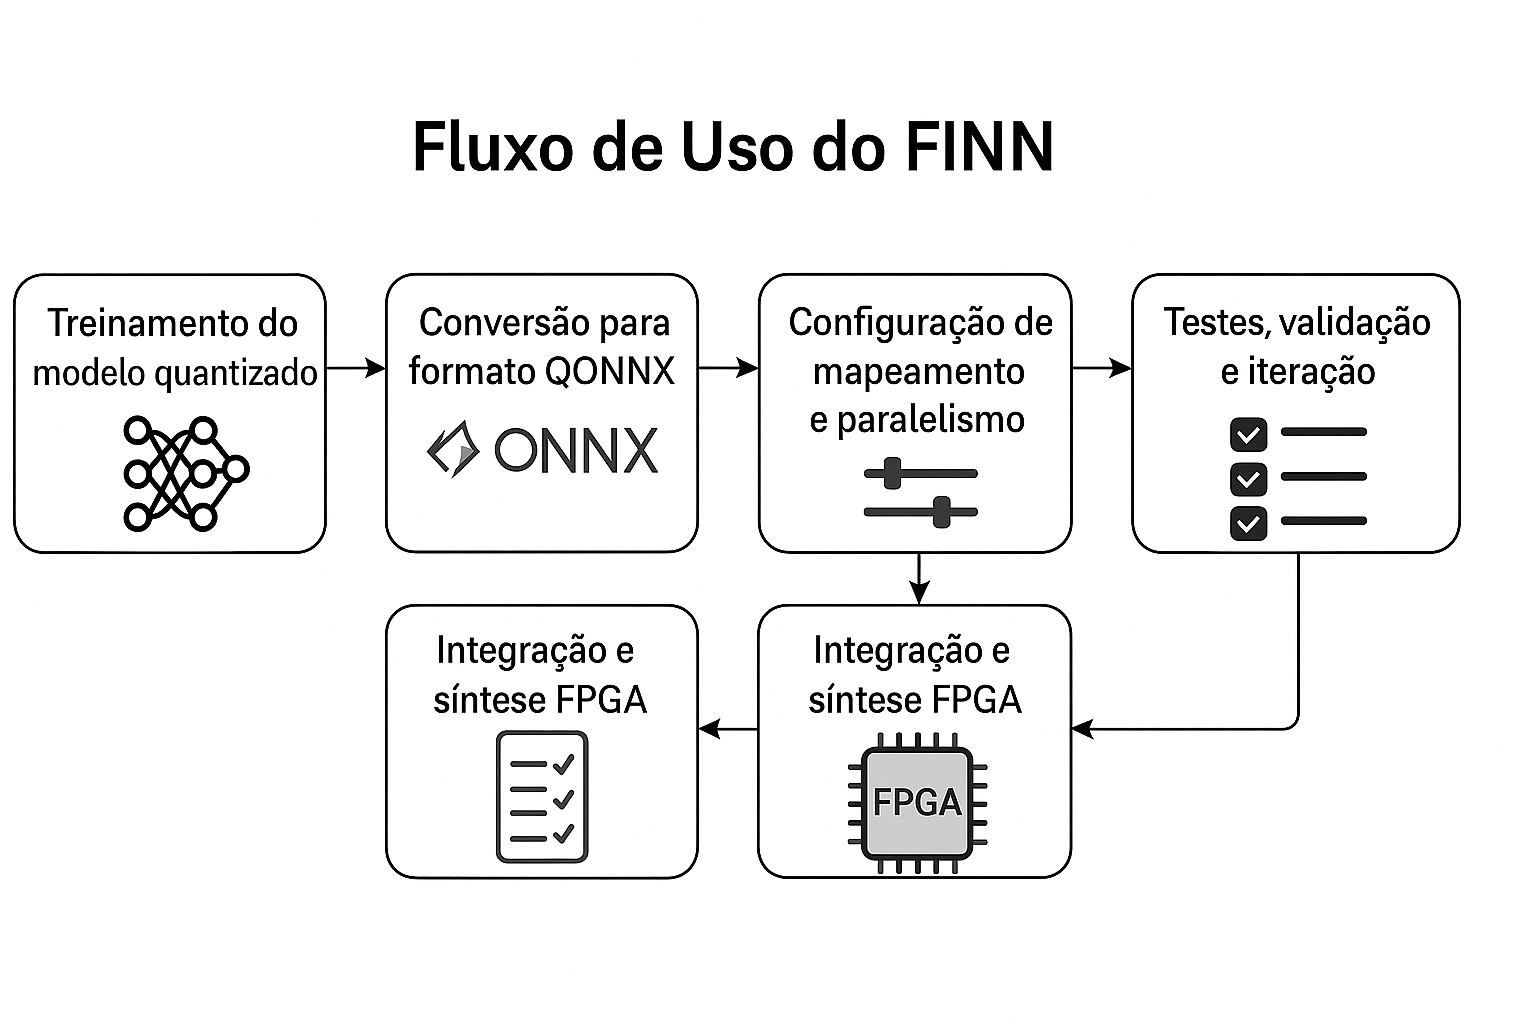
\includegraphics[width=0.80\linewidth]{FluxoUsoFINN.png}
%    \caption{Fluxo do uso do FINN. \\ Fonte: O autor.}
%    \label{fig:FINN_FluxoGeral}
%\end{figure}
%
%O processo se inicia com o \textbf{treinamento de um modelo quantizado}, normalmente conduzido no ambiente \textit{Brevitas}, onde pesos e ativações são ajustados para operar com baixa precisão (por exemplo, 1, 2, 4 ou 8 bits), mantendo a acurácia dentro de margens aceitáveis. Em seguida, o modelo é exportado no formato \textbf{QONNX} (\textit{Quantized Open Neural Network Exchange}), que atua como uma representação intermediária padronizada para a interoperabilidade entre frameworks de aprendizado e \mbox{ferramentas de síntese de hardware.}
%
%Na sequência, o usuário define os parâmetros de \textbf{mapeamento e paralelismo}, determinando a quantidade de unidades de computação, a profundidade de pipeline e o balanceamento entre latência e throughput. O \textbf{FINN Compiler} então converte o modelo quantizado em uma estrutura de hardware equivalente, gerando módulos em HLS ou RTL que representam cada camada da rede neural. Esses módulos são organizados em um fluxo contínuo de dados (\textit{dataflow architecture}), no qual as saídas de uma camada são transmitidas diretamente para a próxima, minimizando a necessidade \mbox{de armazenamento intermediário.}
%
%Após a \textbf{geração dos IPs} (blocos de hardware), o projeto é integrado em ambiente de síntese como o \textit{Vivado} ou o \textit{Vitis}, com conexão via barramento AXI e lógica de controle personalizada. A partir dessa integração, realiza-se a síntese, implementação e geração do \textbf{bitstream}, que configura o FPGA conforme o design projetado.
%
%Finalmente, a etapa de \textbf{teste e validação} avalia o desempenho real do sistema em termos de utilização de recursos, latência, consumo energético e acurácia. Esse processo é iterativo — ajustes finos podem ser aplicados para otimizar o desempenho, explorar paralelismo adicional ou adaptar o hardware a diferentes topologias de rede.
%
%Assim, o diagrama sintetiza o papel do FINN como um elo entre o domínio do aprendizado profundo e o projeto digital reconfigurável, demonstrando como a abstração de alto nível pode ser convertida, de forma automatizada e eficiente, em uma arquitetura física otimizada para execução em FPGA.
%
%
%O FINN também possui extensões importantes, como o \textbf{FINN-R}, um fluxo \textit{end-to-end} de exploração de espaço de design (\textit{Design Space Exploration}) que automatiza a análise de \textit{trade-offs} entre desempenho, consumo e área de hardware, gerando configurações otimizadas de aceleradores personalizados.
%
%Considerando sua capacidade de paralelismo massivo, determinismo temporal e eficiência energética, o FINN consolida-se como uma ferramenta de destaque para a execução de algoritmos de aprendizado profundo em tempo real. Essas características o tornam especialmente adequado para aplicações industriais e embarcadas, nas quais a confiabilidade, a baixa latência e a integração direta com sensores são requisitos fundamentais. Assim, compreender o fluxo de uso do FINN e sua arquitetura interna constitui um passo essencial para o desenvolvimento de sistemas inteligentes de monitoramento e diagnóstico baseados em FPGA.
%
%
%Na subseção seguinte, são apresentados estudos e trabalhos recentes que exploram o uso de FPGAs na aceleração de redes neurais e em aplicações de aprendizado de máquina, evidenciando o estado da arte e as tendências atuais dessa tecnologia no contexto da Inteligência Artificial embarcada.

%\subsection{Aplicações Recentes de FPGAs em Aprendizado de Máquina}
%
%\textcolor{red}{Ainda estou selecionado/lendo/resumindo os artigos}
%\chapter{A Importância e Aplicações da Técnica de Pruning em Redes Neurais Convolucionais}

\section{Introdução}

O crescimento exponencial do uso de redes neurais profundas trouxe avanços significativos em diversas áreas, como reconhecimento de imagem, processamento de sinais, análise de séries temporais, etc. Entretanto, a complexidade e o alto custo computacional dessas redes representam desafios, especialmente em aplicações embarcadas e em tempo real. Nesse contexto, a técnica de pruning (poda) emerge como uma solução eficaz para reduzir a redundância e otimizar o desempenho das redes neurais convolucionais, sem comprometer significativamente a precisão do modelo.

A técnica de pruning (“poda”, em tradução livre) em redes neurais convolucionais (CNNs) consiste na remoção seletiva de parâmetros ou componentes menos relevantes da rede, como conexões, neurônios ou mapas de características. O objetivo é reduzir a complexidade computacional e os requisitos de memória durante a inferência, tornando os modelos mais eficientes sem comprometer significativamente a precisão. Essa técnica é especialmente relevante para aplicações em dispositivos embarcados ou sistemas com restrições de processamento e consumo de energia.

\subsection{Importância do Pruning}

A poda de redes neurais tem um impacto significativo na viabilização do uso de CNNs em ambientes com restrições de hardware, como smartphones, drones e sistemas de visão computacional embarcados. Além disso, reduzir a complexidade computacional da rede pode acelerar a inferência, diminuindo a latência e melhorando a experiência do usuário em aplicações em tempo real.

O artigo "Pruning Convolutional Neural Networks for Resource Efficient Inference" (Molchanov et al., 2017) introduz um método de poda baseado na expansão de Taylor, permitindo a remoção eficiente de mapas de características inteiros sem exigir grande re-treinamento. Esse critério supera abordagens clássicas como Optimal Brain Damage (LeCun et al., 1990) e métodos baseados na magnitude dos pesos, demonstrando correlação mais forte com o critério ótimo de poda (oracle pruning).

Sze et al. (2017) também discutem a importância de técnicas de compressão, como poda e quantização, para tornar redes neurais mais eficientes em diferentes plataformas de hardware, incluindo CPUs, GPUs e FPGAs. Eles destacam que a combinação de pruning e quantização pode reduzir drasticamente a carga computacional sem afetar significativamente a acurácia do modelo.

\subsection{Resultados Obtidos com o Pruning}

Os resultados apresentados por Molchanov et al. (2017) mostram que a poda pode reduzir em mais de 10 vezes o número de operações de convolução em redes adaptadas sem perdas significativas de desempenho. Aplicando a técnica a modelos populares como AlexNet e VGG-16 em tarefas de reconhecimento de imagens (como as bases Birds-200 e Flowers-102), os autores demonstram que:

O método baseado na expansão de Taylor melhora a precisão dos modelos podados em comparação com métodos tradicionais;

A inferência pode ser acelerada em até 3,4x em GPUs modernas e 5,2x em GPUs embarcadas, permitindo uma redução significativa do tempo de processamento;

Redes podadas podem ser executadas com maior eficiência em dispositivos embarcados sem necessidade de hardware especializado.

\subsection{Otimização em FPGA}

A implementação de CNNs em FPGAs é uma solução promissora para aplicações embarcadas, oferecendo alto desempenho com eficiência energética. Zhang et al. (2015) propõem um modelo baseado na técnica roofline, analisando o throughput computacional e a largura de banda necessária para otimizar o uso dos recursos de FPGA. Eles mostram que através de técnicas como loop tiling e transformation, é possível encontrar um equilíbrio entre o uso de memória e capacidade computacional, maximizando a eficiência da execução de CNNs.

A abordagem de Zhang et al. alcançou um desempenho de 61.62 GFLOPS em um FPGA VC707 operando a 100 MHz, superando implementações anteriores. Essa eficiência demonstra o potencial da combinação de pruning e otimizações específicas de FPGA para reduzir consumo de energia e tempo de processamento em dispositivos embarcados.

\subsection{Necessidade do Pruning em Redes Neurais Convolucionais}

As CNNs são caracterizadas por um grande número de parâmetros, principalmente devido às camadas convolucionais e totalmente conectadas. Essa complexidade resulta em:

Alto custo computacional: O treinamento e a inferência de redes profundas exigem grande capacidade de processamento e memória.

Maior consumo de energia: Fundamental para aplicações em dispositivos embarcados e IoT.

Superadaptação: Redes muito complexas podem memorizar padrões irrelevantes dos dados de treinamento, reduzindo sua capacidade de generalização.

Dificuldade na implementação em hardware: Modelos grandes são difíceis de serem implantados em dispositivos com restrições de memória e processamento, como microcontroladores e FPGAs.

O pruning tem o objetivo de mitigar esses problemas, reduzindo a quantidade de parâmetros desnecessários e tornando as redes mais eficientes.

\subsection{Técnicas de Pruning}

Existem diversas abordagens para aplicar pruning em redes neurais convolucionais, sendo as principais:

Pruning baseado em magnitude: Remove conexões cujos pesos têm valores pequenos, assumindo que esses parâmetros contribuem pouco para o resultado final.

Pruning estruturado: Remove neurônios, filtros ou canais inteiros, reduzindo significativamente o tamanho da rede e o custo computacional.

Pruning não estruturado: Remove conexões individuais sem comprometer a estrutura global da rede, exigindo hardware especializado para obter ganhos reais de eficiência.

Pruning dinâmico: Remove pesos durante o treinamento e pode reintroduzi-los conforme necessário, ajustando dinamicamente a arquitetura.

Pruning iterativo: Aplica a remoção de parâmetros em múltiplas etapas, com reaferimento da rede para manter o desempenho.

\subsection{Pruning em CNNs e CNN1D}

As CNNs tradicionais (2D) são amplamente utilizadas em processamento de imagens, enquanto as CNN1D são empregadas no processamento de sinais e séries temporais. Ambas se beneficiam do pruning, com algumas diferenças importantes:

CNNs (2D): A poda de filtros convolucionais pode reduzir significativamente a complexidade, mantendo a capacidade de extração de padrões espaço-temporais.

CNN1D: Muito utilizadas em sinais biomédicos, financeiros e acústicos, a remoção de canais irrelevantes pode acelerar a inferência sem perda significativa de informação.

Aplicações Práticas do Pruning

Visão Computacional: Redução do tamanho de redes como ResNet e VGG para execução eficiente em dispositivos móveis.

Processamento de Sinais Biomédicos: Análise de ECG e EEG utilizando CNN1D, reduzindo o tempo de inferência sem comprometer a acurácia do diagnóstico.

Detecção de Falhas em Equipamentos: Pruning em CNN1D para análise de sinais acústicos, possibilitando inferência em tempo real.

Edge Computing e IoT: Implementação de modelos eficientes em hardwares embarcados, como FPGAs e microcontroladores.

Conclusão

A técnica de pruning é essencial para a eficiência de redes neurais convolucionais, permitindo execução otimizada em ambientes com restrições computacionais. Seu uso em CNNs e CNN1D tem impulsionado avanços em diversas áreas, desde a visão computacional até a análise de sinais biomédicos e acústicos. Com a crescente demanda por modelos mais eficientes, espera-se que novas abordagens de pruning sejam desenvolvidas para maximizar a relação entre desempenho e eficiência computacional.

%\chapter{Trabalhos Relacionados}
\section{Aprendizado de Máquina com Emissão Acústica para Detecção de Falhas}

\subsection{Introdução}

A Emissão Acústica (EA) é uma técnica consolidada para a detecção de falhas em materiais e estruturas. Nos últimos anos, o uso de aprendizado de máquina (ML, do inglês Machine Learning) em combinação com EA tem se mostrado promissor, especialmente para melhorar a precisão e a automação da detecção de falhas. O aprendizado de máquina permite identificar padrões complexos em dados acústicos que seriam difíceis de detectar manualmente, tornando-o uma abordagem inovadora para o monitoramento preditivo e a manutenção de ativos críticos.

\subsection{História do Uso de Aprendizado de Máquina com Emissão Acústica}

A combinação de aprendizado de máquina e EA para detecção de falhas é relativamente recente. O uso de EA começou a se popularizar na década de 1950, mas foi apenas com os avanços em processamento de sinais e inteligência artificial, a partir das décadas de 1990 e 2000, que surgiram as primeiras tentativas de integrar técnicas de aprendizado de máquina ao processo de análise de sinais de EA (Pollock, 2012).
O desenvolvimento de algoritmos supervisionados, como redes neurais artificiais, e de técnicas não supervisionadas, como agrupamento (clustering), possibilitou a criação de sistemas automáticos de detecção de falhas baseados em EA. Mais recentemente, com o aumento da capacidade computacional e o advento de métodos mais avançados de aprendizado, como deep learning, a análise de grandes volumes de dados acústicos tornou-se mais eficiente e precisa (Sohn et al., 2010).

\subsection{Fundamentos do Aprendizado de Máquina e Emissão Acústica}

A Emissão Acústica é um método não destrutivo que detecta ondas acústicas geradas por eventos internos em materiais. Essas ondas, ao serem captadas por sensores piezoelétricos, geram sinais complexos, cuja análise pode fornecer informações sobre a presença e a localização de falhas, como trincas, corrosão ou fadiga.

Com o aprendizado de máquina, esses sinais de EA podem ser processados de maneira mais robusta. As técnicas de ML são usadas para:


Classificação: Identificar automaticamente se os eventos acústicos indicam uma falha ou se são ruídos ou outros eventos normais.


Detecção de Anomalias: Sistemas não supervisionados de aprendizado de máquina podem ser treinados para detectar padrões anômalos em dados de EA, indicando a possível presença de falhas incipientes.


Previsão: Técnicas de regressão e redes neurais são aplicadas para prever a progressão de uma falha com base no histórico de sinais de EA.
Essas abordagens têm uma vantagem significativa em relação aos métodos tradicionais de análise de sinais, pois podem aprender a identificar padrões complexos sem a necessidade de definir previamente regras rígidas, o que as torna mais adaptáveis a diferentes materiais e condições operacionais (Aggelis et al., 2012).

\subsection{Aplicações de Aprendizado de Máquina com Emissão Acústica}

Monitoramento Estrutural em Tempo Real
Um dos principais campos de aplicação é o monitoramento de grandes estruturas, como pontes e edifícios. Sensores de EA acoplados a sistemas de aprendizado de máquina podem detectar a propagação de trincas em tempo real. A capacidade de ML de reconhecer padrões complexos em sinais de EA ajuda a distinguir eventos críticos de ruídos de fundo, fornecendo alertas precoces para intervenções (Sharma et al., 2021).

\subsubsection{Indústria Aeroespacial}

Na indústria aeroespacial, o aprendizado de máquina tem sido usado para analisar sinais de EA captados de componentes críticos, como fuselagens e asas de aeronaves. Modelos de ML treinados com dados históricos de falhas podem identificar possíveis defeitos causados por fadiga de materiais, garantindo maior segurança (Prosser, 1991).

\subsubsection{Manutenção Preditiva de Máquinas Rotativas}

Máquinas rotativas, como turbinas, motores e bombas, também se beneficiam dessa integração. O aprendizado de máquina pode classificar sinais de EA captados de rolamentos e eixos para identificar desgaste, desalinhamento e cavitação. Ao usar técnicas de detecção de anomalias, os sistemas podem prever falhas antes que elas ocorram, reduzindo o tempo de inatividade e custos de manutenção (Gupta et al., 2017).

\subsubsection{Monitoramento de Corrosão}

Sistemas de ML aplicados à detecção de corrosão usando EA são capazes de identificar o início de processos corrosivos em materiais metálicos, como em tubulações e estruturas offshore. A sensibilidade desses sistemas permite detectar os primeiros sinais de corrosão por pite, ajudando na preservação de infraestruturas críticas (Chaudhry et al., 1997).

\subsection{Desafios e Oportunidades}

Apesar dos avanços, a aplicação de aprendizado de máquina em EA enfrenta alguns desafios. Um dos principais problemas é a necessidade de grandes volumes de dados etiquetados para treinar modelos supervisionados. A aquisição de tais dados pode ser cara e demorada, especialmente em ambientes industriais onde as falhas ocorrem com pouca frequência. Outro desafio é a presença de ruídos, que pode comprometer a precisão dos modelos de ML.
Com o aumento da capacidade de coleta e processamento de dados em tempo real, há uma oportunidade crescente de aplicar modelos mais complexos, como redes neurais profundas, para melhorar a detecção de falhas. Além disso, o uso de técnicas de aprendizado por reforço e aprendizado federado pode permitir a criação de sistemas mais adaptáveis e distribuídos, que aprendem continuamente à medida que novos dados são coletados (Zhu et al., 2020).

\subsubsection{Conclusão}
A combinação de aprendizado de máquina e Emissão Acústica representa uma evolução significativa no campo da detecção de falhas. Essa integração permite monitoramento em tempo real, predição precisa e automação de processos, tornando-a uma ferramenta valiosa para a indústria 4.0 e para sistemas de manutenção preditiva. Com o avanço contínuo dos algoritmos de ML e das tecnologias de sensoriamento, espera-se que essa abordagem se torne ainda mais robusta e amplamente aplicável em uma variedade de indústrias.

% 3.8.	Referências
% Aggelis, D. G., Verbruggen, S., Tsangouri, E., & Tysmans, T. (2012). Monitoring of crack propagation in a concrete beam during four-point bending by combined techniques. NDT & E International, 48, 66-72. 
% Chaudhry, Z., Gan, D. D., & Raghavan, V. (1997). Acoustic emission monitoring of corrosion in metallic structures. Journal of Engineering Materials and Technology, 119(2), 192-198. 
% Gupta, M. S., Behera, D. K., & Nayak, A. K. (2017). Acoustic emission-based condition monitoring of rotating machines: A review. Engineering Failure Analysis, 79, 626-642.

% Pollock, A. A. (2012). Fundamentals of acoustic emission testing. Journal of Acoustic Emission, 30(2), 55-69. 
% Prosser, W. H. (1991). Advanced AE techniques in composite materials research. Journal of Acoustic Emission, 9(4), 292-306.
% Sharma, N., Chakraborty, S., & Chowdhury, R. (2021). Fault detection using machine learning algorithms in structural health monitoring: A review. Journal of Civil Structural Health Monitoring, 11, 1065-1091.
% Sohn, H., Dutta, D., & Taylor, S. G. (2010). Acoustic emission monitoring for crack detection and localization in plate structures. Nondestructive Testing and Evaluation, 25(4), 321-331.
% Zhu, M., Wang, Z., Xu, Y., & Zhang, T. (2020). An overview of federated learning. Journal of Nondestructive Testing, 40, 1231-1245.

%\chapter{Uso e Implementação de Deep Learning em FPGA}

O avanço das redes neurais profundas (Deep Learning) tem revolucionado áreas como visão computacional, reconhecimento de padrões e processamento de sinais. No entanto, a alta demanda computacional dessas técnicas exige plataformas de hardware eficientes para sua execução, especialmente em cenários que requerem baixo consumo de energia e alta velocidade de processamento. Os Field Programmable Gate Arrays (FPGAs) emergiram como uma solução promissora devido à sua flexibilidade, eficiência energética e capacidade de paralelismo. Este texto explora o uso e a implementação de Deep Learning em FPGAs, com foco em Convolutional Neural Networks (CNNs) e Long Short-Term Memory (LSTM), utilizando como base teórica e fonte de resultados três artigos acadêmicos: um da SET EXPO Proceedings (Aguirre e Jerji, 2022), um da Neural Computing and Applications (Mittal, 2018) e outro da Sensors (Wu et al., 2024).

\section{Fundamentos do Uso de FPGAs em Deep Learning}
Os FPGAs são dispositivos reconfiguráveis que oferecem vantagens significativas sobre processadores tradicionais como CPUs e GPUs em aplicações específicas de Deep Learning. Conforme destacado por Mittal (2018), os FPGAs proporcionam maior eficiência energética e desempenho superior às CPUs, além de flexibilidade em comparação com Application-Specific Integrated Circuits (ASICs). Sua arquitetura permite a implementação de operações paralelas, essenciais para redes neurais, utilizando recursos como Look-Up Tables (LUTs), Block RAMs (BRAMs) e Digital Signal Processing units (DSPs).

Aguirre e Jerji (2022) enfatizam que os avanços recentes em FPGAs, como maior capacidade de processamento paralelo e ferramentas de síntese de alto nível (High-Level Synthesis - HLS), como o Xilinx Vivado, tornaram-nos candidatos ideais para acelerar redes neurais. Essas ferramentas reduzem a complexidade do design, permitindo a compilação de código de alto nível para especificações de Register Transfer Level (RTL), o que facilita a implementação por desenvolvedores sem expertise avançada em hardware.

Por fim, Wu et al. (2024) demonstram que os FPGAs são particularmente úteis em aplicações que demandam baixo consumo energético e processamento em tempo real, como o reconhecimento de sinais de emissores de radar. A combinação de reconfigurabilidade e eficiência energética torna os FPGAs uma plataforma versátil para diferentes modelos de Deep Learning.

\section{Implementação de Convolutional Neural Networks (CNNs) em FPGAs}
As CNNs, amplamente utilizadas em tarefas de reconhecimento de imagens e sinais, requerem operações intensivas como convoluções e multiplicações matriz-vetor. A implementação dessas redes em FPGAs tem sido explorada para otimizar desempenho e eficiência.

\subsection{Estrutura e Otimizações}
Mittal (2018) descreve que as CNNs em FPGAs enfrentam desafios como a limitação de memória on-chip para armazenar parâmetros (e.g., AlexNet requer ~250 MB). Para contornar isso, técnicas como loop unrolling, pipelining e tiling são empregadas. O loop unrolling explora o paralelismo entre iterações, enquanto o pipelining permite que operações subsequentes comecem antes do término das anteriores, aumentando o throughput. O tiling particiona os dados em blocos menores para otimizar o uso da memória cache.

Aguirre e Jerji (2022) detalham a implementação de uma CNN em FPGA para reconhecimento de imagens usando o dataset MNIST. Eles utilizaram VHDL para criar blocos modulares (e.g., TOP, neuron, layer) e testaram diferentes configurações, como número de camadas e precisão numérica (inteiros vs. ponto fixo). Os resultados mostram que a precisão de três casas decimais e o uso de LUTs para funções de ativação (e.g., sigmoid) reduzem o tempo de resposta sem sacrificar acurácia, alcançando tempos de 23,77 a 27,37 µs em uma placa Basys 3 Artix-7 com clock de 100 MHz.

\subsection{Aplicações Específicas}
Wu et al. (2024) propõem uma CNN unidimensional (1D-CNN) combinada com LSTM para reconhecimento de sinais de radar. A CNN extrai características locais dos dados de frequência intermediária (IF), utilizando quatro camadas convolucionais com kernels de tamanho 15 e pooling máximo. A implementação em FPGA (Xilinx XCKU040) utiliza um array sistólico de 32x64 para acelerar operações de convolução 1D, alcançando um throughput de 7,34 GOPS com consumo de 5,022 W e acurácia de 96,53%. Essa abordagem demonstra a capacidade dos FPGAs em processar sinais de comprimento variável em tempo real.

\subsection{Integração de Long Short-Term Memory (LSTM) em FPGAs}
As redes LSTM, um tipo de Recurrent Neural Network (RNN), são projetadas para modelar dependências temporais, sendo ideais para sequências como sinais de radar. Sua implementação em FPGAs apresenta desafios adicionais devido à natureza sequencial das operações.

\subsection{Design e Aceleração}
Wu et al. (2024) integram uma camada LSTM após a CNN em seu modelo 1D-CNN-LSTM. O array sistólico é reutilizado para multiplicações matriz-vetor, e as funções de ativação (sigmoid e tanh) são implementadas via tabelas de consulta (LUTs) em ROM, reduzindo o custo computacional. A flexibilidade do modelo permite lidar com variações no comprimento dos pulsos de radar (1-10 µs), mantendo uma acurácia acima de 55% mesmo fora do intervalo de treinamento (1-5 µs).

Aguirre e Jerji (2022) não exploram diretamente LSTMs, mas sua abordagem de design flexível em VHDL poderia ser adaptada para incluir camadas recorrentes, ajustando o número de neurônios e camadas via código reconfigurável.

\subsection{Benefícios e Limitações}
A integração CNN-LSTM em Wu et al. (2024) destaca a eficiência energética (1,46 GOPS/W) em comparação com CPUs (0,02 GOPS/W) e GPUs (0,16 GOPS/W), embora o throughput absoluto seja menor que o de GPUs (7,34 vs. 16,73 GOPS). Mittal (2018) aponta que a natureza sequencial das RNNs pode limitar o paralelismo total em FPGAs, sugerindo otimizações como folding temporal ou espacial para redes maiores.

\subsection{Comparação com Outras Plataformas e Resultados}
Os artigos analisados comparam o desempenho dos FPGAs com CPUs e GPUs. Aguirre e Jerji (2022) mostram que sua CNN em FPGA tem um tempo de resposta de 25,17 µs, muito inferior aos 20 ms em uma CPU Intel i7-6700K e 18 ms em uma GPU Nvidia GTX 980TI, evidenciando a vantagem em aplicações de baixa latência, como veículos autônomos. Wu et al. (2024) reforçam essa superioridade em eficiência energética, crucial para dispositivos embarcados. Mittal (2018) observa que, embora GPUs ofereçam maior throughput bruto, os FPGAs superam em cenários de energia limitada e permitem atualizações rápidas via reconfiguração, ao contrário dos ASICs.

\section{\textcolor{red}{Uso de Aprendizado de Máquina Embarcado em FPGA para Análise de Dados de Emissão Acústica na Detecção de Falhas}}

\subsection{Introdução}

A detecção de falhas é uma área crítica em diversas indústrias, desde o setor aeroespacial até a infraestrutura civil. A combinação da técnica de Emissão Acústica (EA) com algoritmos de Aprendizado de Máquina (ML) tem mostrado grande potencial para melhorar a precisão e a eficiência na identificação de falhas incipientes. Além disso, a implementação de sistemas embarcados baseados em Field-Programmable Gate Arrays (FPGA) oferece uma solução otimizada para o processamento em tempo real dos dados de EA, superando as limitações de sistemas tradicionais baseados em software. Este artigo examina a evolução do uso de aprendizado de máquina embarcado em FPGAs para análise de dados de EA, bem como suas aplicações e desafios.

\subsection{História do Uso de FPGAs e Aprendizado de Máquina com Emissão Acústica}

A Emissão Acústica como técnica de monitoramento de falhas foi amplamente adotada a partir da década de 1950 (Kaiser, 1950). No entanto, o desenvolvimento de sistemas embarcados para processar esses dados de forma eficiente começou a ganhar tração nas décadas de 1990 e 2000, com a evolução dos FPGAs como plataformas programáveis para processamento de sinais digitais (DSP) (Benkrid et al., 2008). Com o avanço das técnicas de aprendizado de máquina, tornou-se possível implementar algoritmos complexos diretamente em hardware, proporcionando uma análise em tempo real com baixa latência e alto desempenho, características fundamentais para monitoramento preditivo.

O uso de FPGAs para implementar aprendizado de máquina surgiu como uma alternativa a processadores de propósito geral devido à capacidade de paralelismo massivo, flexibilidade e eficiência energética, o que é essencial em aplicações que demandam alta taxa de amostragem e processamento contínuo de grandes volumes de dados, como é o caso da Emissão Acústica (Marino et al., 2018).

\subsection{Conclusão}
A combinação de aprendizado de máquina embarcado em FPGA e Emissão Acústica é uma abordagem poderosa para a detecção de falhas em tempo real. O uso de FPGAs oferece vantagens claras em termos de desempenho e eficiência energética, enquanto o aprendizado de máquina permite uma análise precisa e automatizada dos dados de EA. Com o avanço contínuo nas tecnologias de FPGA e nas técnicas de aprendizado de máquina, essa abordagem está se tornando cada vez mais essencial para aplicações de monitoramento preditivo e manutenção de ativos críticos.

% 4.10.	Referências
% •	Beattie, A. G. (1995). Acoustic emission monitoring of metal fatigue. NASA STI/Recon Technical Report N.
% •	Benkrid, K., Crookes, D., & Erdogan, A. T. (2008). FPGA architectures for high-performance computing. Journal of Parallel and Distributed Computing, 68(4), 501-517.
% •	Grosse, C., & Ohtsu, M. (2008). Acoustic Emission Testing. Springer.
% •	Kaiser, J. (1950). Untersuchung über das Auftreten von Geräuschen beim Zugversuch (Doctoral dissertation, Technische Hochschule München).
% •	Marino, D., San Miguel, J. M., & Kurkovsky, S. (2018). Power-efficient FPGA-based acceleration of deep learning algorithms for image processing. ACM Transactions on Embedded Computing Systems, 17(3), 1-23.
% •	Prosser, W. H. (1991). Advanced AE techniques in composite materials research. Journal of Acoustic Emission, 9(4), 292-306.
% •	Sulaiman, M., Naeem, M., & Ahmed, S. (2021). FPGA-based architectures for deep learning applications: A survey. IEEE Access, 9, 14584-14598.
% •	Zhao, L., Wang, Y., Xu, X., & Zhang, Y. (2023). Edge computing with FPGAs: Emerging trends and future directions. ACM Computing Surveys, 55(1), 1-33.
% •	Zhu, M., Wang, Z., Xu, Y., & Zhang, T. (2020). An overview of federated learning. Journal of Nondestructive Testing, 40, 1231-1245.



% ----------------------------------------------------------
% PARTE
% ----------------------------------------------------------
%\part{Preparação da pesquisa}
% ----------------------------------------------------------

% ----------------------------------------------------------
% PARTE
% ----------------------------------------------------------
%\part{Referenciais teóricos}
% ----------------------------------------------------------

% ---
% Capitulo de revisão de literatura
% ---
%\chapter{Lorem ipsum dolor sit amet}
% ---

% ---
%\section{Aliquam vestibulum fringilla lorem}
% ---

%\lipsum[1]

%\lipsum[2-3]


% ----------------------------------------------------------
% Finaliza a parte no bookmark do PDF
% para que se inicie o bookmark na raiz
% e adiciona espaço de parte no Sumário
% ----------------------------------------------------------
\phantompart

% ----------------------------------------------------------
% ELEMENTOS PÓS-TEXTUAIS
% ----------------------------------------------------------
\postextual
% ----------------------------------------------------------

% ----------------------------------------------------------
% Referências bibliográficas
% ----------------------------------------------------------
\bibliography{bibliografia}



% ----------------------------------------------------------
% Glossário
% ----------------------------------------------------------
%
% Consulte o manual da classe abntex2 para orientações sobre o glossário.
%
%\glossary

% ----------------------------------------------------------
% Apêndices
% ----------------------------------------------------------

% ---
% Inicia os apêndices
% ---
% \begin{apendicesenv}

% Imprime uma página indicando o início dos apêndices
% \partapendices

% % ----------------------------------------------------------
% \chapter{Quisque libero justo}
% % ----------------------------------------------------------

% \lipsum[50]

% % ----------------------------------------------------------
% \chapter{Nullam elementum urna vel imperdiet sodales elit ipsum pharetra ligula
% ac pretium ante justo a nulla curabitur tristique arcu eu metus}
% % ----------------------------------------------------------
% \lipsum[55-57]

% \end{apendicesenv}
% ---


% ----------------------------------------------------------
% Anexos
% ----------------------------------------------------------

% ---
% Inicia os anexos
% ---
% \begin{anexosenv}

% Imprime uma página indicando o início dos anexos
% \partanexos

% ---
%\chapter{Morbi ultrices rutrum lorem.}
% ---
%\lipsum[30]

% ---
%\chapter{Cras non urna sed feugiat cum sociis natoque penatibus et magnis dis
%parturient montes nascetur ridiculus mus}
% ---

%\lipsum[31]

% ---
%\chapter{Fusce facilisis lacinia dui}
% ---

%\lipsum[32]

% \end{anexosenv}

%---------------------------------------------------------------------
% INDICE REMISSIVO
%---------------------------------------------------------------------
\phantompart
\printindex
%---------------------------------------------------------------------

\end{document}
